\section{Results}

\subsection{Communication}

As shown in TABLE \ref{tab:UDPMeasurements}, when the frequency increases from 100 Hz to 500 Hz, so does\todo{do?} the jitter and packet loss. However when the refresh rate is increased to its maximum value the jitter sharply decreases while the packet loss increases significantly.

 % It was stated before that the requirements for our system was to get to at least 550 Hz and to reach 1000Hz if possible. As shown in Table \ref{tab:UDPMeasurements}, the connection can go up to almost 1000Hz using UDP which fulfills the requirements. However, the jitter should not be neglected as the frequency get closer to 1000Hz the jitter increases and becomes high compared to the period and may cause unexpected behavior in real time operation. It is though that as the period become smaller, the system becomes more sensitive to the preemption of other processes.
\begin{center}
  $\begin{tabular}{|c|c|c|c|c|c|}
    \hline
    \text{Frequency (Hz)} & \text{delay (ms)} & \text{Jitter ($\mu$s)} & \text{Packet loss (\%)}\\
    \hline
    99 & 10.1 & 4.66E-2 & 0 \\
    \hline
    474 & 2.1 & 5.51E-2 & 0.2 \\
    \hline
    638 & 1.6 & 1.16E-2 & 1.2 \\
    \hline
  \end{tabular}$
  \captionof{table}{Measurements of the UDP performances}
  \label{tab:UDPMeasurements}
\todo{2 columns are redundant, maybe put the set frequency instead}
\end{center}
The goal of 1000 Hz could not be reached when running the entire system. However, as the original communication could not exceed the refresh rate of 100Hz a significant improvement is to be noted.

\begin{figure}[h]
  % This file was created by matlab2tikz.
%
%The latest updates can be retrieved from
%  http://www.mathworks.com/matlabcentral/fileexchange/22022-matlab2tikz-matlab2tikz
%where you can also make suggestions and rate matlab2tikz.
%
\definecolor{mycolor1}{rgb}{0.00000,0.44700,0.74100}%
\definecolor{mycolor2}{rgb}{0.85000,0.32500,0.09800}%
%
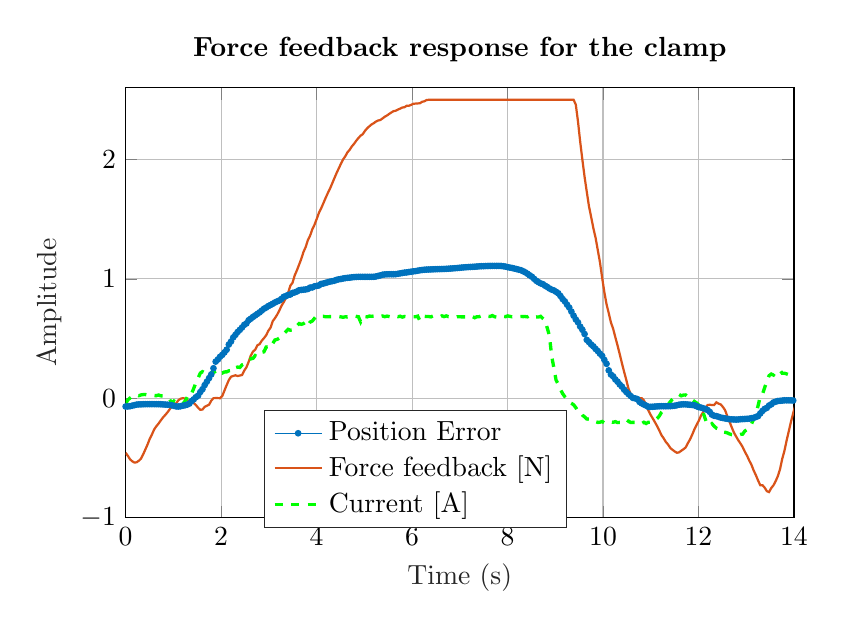
\begin{tikzpicture}

\begin{axis}[%
width=0.7\columnwidth,
height=0.45\columnwidth,
at={(2.512in,1.147in)},
scale only axis,
xmin=0,
xmax=14,
xlabel style={font=\color{white!15!black}},
xlabel={Time (s)},
ymin=-1,
ymax=2.6,
ylabel style={font=\color{white!15!black}},
ylabel={Amplitude},
axis background/.style={fill=white},
title style={font=\bfseries},
title={Force feedback response for the clamp},
xmajorgrids,
ymajorgrids,
legend style={legend cell align=left, align=left, draw=white!15!black, at={(0.66,0.25)}}
]
\addplot [color=mycolor1, draw=none, mark=*, mark size=1,mark options={solid, mycolor1}]
  table[row sep=crcr]{%
0	-0.069839\\
0.046	-0.0691929999999998\\
0.092	-0.0674169999999998\\
0.138	-0.0627580000000001\\
0.184	-0.0585599999999999\\
0.23	-0.053715\\
0.276	-0.052262\\
0.322	-0.0517779999999999\\
0.368	-0.0508089999999999\\
0.414	-0.050325\\
0.46	-0.0500019999999999\\
0.506	-0.0500019999999999\\
0.552	-0.0500019999999999\\
0.598	-0.0500019999999999\\
0.644	-0.050233\\
0.69	-0.0504629999999999\\
0.736	-0.0509360000000001\\
0.782	-0.0523979999999999\\
0.828	-0.0533170000000001\\
0.874	-0.0544640000000001\\
0.92	-0.0558380000000001\\
0.966	-0.059431\\
1.012	-0.0646089999999999\\
1.058	-0.069102\\
1.104	-0.070166\\
1.15	-0.0678619999999999\\
1.196	-0.0632820000000001\\
1.242	-0.0596559999999999\\
1.288	-0.054314\\
1.334	-0.045984\\
1.38	-0.0253700000000001\\
1.426	-0.00976399999999988\\
1.472	0.00805999999999996\\
1.518	0.0212249999999999\\
1.564	0.051482\\
1.61	0.0750869999999999\\
1.656	0.109672\\
1.702	0.138343\\
1.748	0.168177\\
1.794	0.199188\\
1.84	0.250473\\
1.886	0.306211\\
1.932	0.324103\\
1.978	0.347052\\
2.024	0.362787\\
2.07	0.383776\\
2.116	0.406007\\
2.162	0.449559\\
2.208	0.474824\\
2.254	0.508958\\
2.3	0.530804\\
2.346	0.554437\\
2.392	0.572537\\
2.438	0.591942\\
2.484	0.614258\\
2.53	0.625926\\
2.576	0.652916\\
2.622	0.665954\\
2.668	0.680707\\
2.714	0.6931054\\
2.76	0.7064931\\
2.806	0.7187228\\
2.852	0.7341136\\
2.898	0.7492224\\
2.944	0.7593239\\
2.99	0.7720971\\
3.036	0.7809118\\
3.082	0.7910974\\
3.128	0.8020223\\
3.174	0.81066\\
3.22	0.8186307\\
3.266	0.8319814\\
3.312	0.8492741\\
3.358	0.8558223\\
3.404	0.8646376\\
3.45	0.868742\\
3.496	0.8814436\\
3.542	0.8863328\\
3.588	0.8938385\\
3.634	0.9044656\\
3.68	0.9069801\\
3.726	0.9089659\\
3.772	0.9109976\\
3.818	0.9148639\\
3.864	0.9265554\\
3.91	0.9278963\\
3.956	0.9373217\\
4.002	0.940841\\
4.048	0.9445568\\
4.094	0.95726415\\
4.14	0.9604788\\
4.186	0.96597617\\
4.232	0.97119919\\
4.278	0.97641396\\
4.324	0.9801821\\
4.37	0.9838232\\
4.416	0.9907857\\
4.462	0.99572\\
4.508	0.9983443\\
4.554	1.0027004\\
4.6	1.0057562\\
4.646	1.0081051\\
4.692	1.0098843\\
4.738	1.0125273\\
4.784	1.0145615\\
4.83	1.015724\\
4.876	1.0164667\\
4.922	1.0164667\\
4.968	1.0164667\\
5.014	1.0164667\\
5.06	1.0164667\\
5.106	1.0164667\\
5.152	1.0164667\\
5.198	1.017048\\
5.244	1.0196638\\
5.29	1.0246052\\
5.336	1.0286748\\
5.382	1.0344887\\
5.428	1.0368141\\
5.474	1.0379768\\
5.52	1.0385582\\
5.566	1.0385582\\
5.612	1.0385582\\
5.658	1.0391396\\
5.704	1.0420462\\
5.75	1.045534\\
5.796	1.0490214\\
5.842	1.0522178\\
5.888	1.0536705\\
5.934	1.0571568\\
5.98	1.059633\\
6.026	1.062445\\
6.072	1.0644935\\
6.118	1.0679936\\
6.164	1.0718006\\
6.21	1.0739226\\
6.256	1.0760766\\
6.302	1.0773746\\
6.348	1.0781606\\
6.394	1.0786866\\
6.44	1.0796386\\
6.486	1.0806226\\
6.532	1.0811326\\
6.578	1.0815816\\
6.624	1.0821676\\
6.67	1.0826356\\
6.716	1.0836156\\
6.762	1.0849286\\
6.808	1.0862066\\
6.854	1.0874876\\
6.9	1.0889816\\
6.946	1.0904386\\
6.992	1.0921886\\
7.038	1.0943516\\
7.084	1.0958206\\
7.13	1.0971756\\
7.176	1.0983656\\
7.222	1.0995076\\
7.268	1.1005966\\
7.314	1.1015086\\
7.36	1.1031166\\
7.406	1.1045566\\
7.452	1.1057716\\
7.498	1.1059546\\
7.544	1.1072416\\
7.59	1.1076566\\
7.636	1.1080086\\
7.682	1.1083606\\
7.728	1.1083606\\
7.774	1.1082496\\
7.82	1.1082496\\
7.866	1.1078506\\
7.912	1.1055066\\
7.958	1.1023436\\
8.004	1.0977176\\
8.05	1.0940366\\
8.096	1.0909596\\
8.142	1.0861036\\
8.188	1.0816106\\
8.234	1.0766646\\
8.28	1.0723386\\
8.326	1.0637863\\
8.372	1.0543818\\
8.418	1.0428257\\
8.464	1.029448\\
8.51	1.0175659\\
8.556	1.0002029\\
8.602	0.9837055\\
8.648	0.97187785\\
8.694	0.96156563\\
8.74	0.9554396\\
8.786	0.942303\\
8.832	0.9318928\\
8.878	0.9191614\\
8.924	0.9095359\\
8.97	0.9029574\\
9.016	0.8912888\\
9.062	0.879097\\
9.108	0.8563865\\
9.154	0.8307516\\
9.2	0.8113894\\
9.246	0.7837317\\
9.292	0.7592755\\
9.338	0.725409\\
9.384	0.691096\\
9.43	0.659743\\
9.476	0.635184\\
9.522	0.599631\\
9.568	0.572746\\
9.614	0.537474\\
9.66	0.488529\\
9.706	0.470013\\
9.752	0.449131\\
9.798	0.434072\\
9.844	0.412879\\
9.89	0.394881\\
9.936	0.372667\\
9.982	0.354272\\
10.028	0.320757\\
10.074	0.287993\\
10.12	0.232964\\
10.166	0.197741\\
10.212	0.18275\\
10.258	0.156795\\
10.304	0.138484\\
10.35	0.114872\\
10.396	0.097008\\
10.442	0.071595\\
10.488	0.05155\\
10.534	0.034095\\
10.58	0.0179400000000001\\
10.626	0.002305\\
10.672	-0.00167099999999998\\
10.718	-0.00769699999999984\\
10.764	-0.030978\\
10.81	-0.0429710000000001\\
10.856	-0.053148\\
10.902	-0.0618189999999998\\
10.948	-0.0720810000000001\\
10.994	-0.0724389999999999\\
11.04	-0.0717700000000001\\
11.086	-0.0703040000000001\\
11.132	-0.068948\\
11.178	-0.0678830000000001\\
11.224	-0.067339\\
11.27	-0.067339\\
11.316	-0.067339\\
11.362	-0.0671580000000001\\
11.408	-0.0669960000000001\\
11.454	-0.065239\\
11.5	-0.063358\\
11.546	-0.0595410000000001\\
11.592	-0.054964\\
11.638	-0.052603\\
11.684	-0.051604\\
11.73	-0.0518610000000002\\
11.776	-0.053331\\
11.822	-0.0551919999999999\\
11.868	-0.0570810000000002\\
11.914	-0.059763\\
11.96	-0.0673490000000001\\
12.006	-0.075137\\
12.052	-0.0787260000000001\\
12.098	-0.084632\\
12.144	-0.090457\\
12.19	-0.099099\\
12.236	-0.115104\\
12.282	-0.138322\\
12.328	-0.147654\\
12.374	-0.150269\\
12.42	-0.156016\\
12.466	-0.1626\\
12.512	-0.166108\\
12.558	-0.169979\\
12.604	-0.172681\\
12.65	-0.176454\\
12.696	-0.177723\\
12.742	-0.178345\\
12.788	-0.179376\\
12.834	-0.178237\\
12.88	-0.176378\\
12.926	-0.175254\\
12.972	-0.174123\\
13.018	-0.172999\\
13.064	-0.171682\\
13.11	-0.167706\\
13.156	-0.164679\\
13.202	-0.157745\\
13.248	-0.1501\\
13.294	-0.127712\\
13.34	-0.106903\\
13.386	-0.0901689999999999\\
13.432	-0.0812360000000001\\
13.478	-0.0620539999999998\\
13.524	-0.0516510000000001\\
13.57	-0.035822\\
13.616	-0.029779\\
13.662	-0.0236429999999999\\
13.708	-0.0221900000000002\\
13.754	-0.0202520000000002\\
13.8	-0.0181120000000001\\
13.846	-0.018038\\
13.892	-0.018243\\
13.938	-0.0184470000000001\\
13.984	-0.019682\\
14.03	-0.0207010000000001\\
14.076	-0.0221230000000001\\
14.122	-0.023096\\
14.168	-0.023096\\
14.214	-0.023096\\
14.26	-0.0234529999999999\\
14.306	-0.024132\\
14.352	-0.0254239999999999\\
14.398	-0.0299449999999999\\
14.444	-0.033693\\
14.49	-0.0363100000000001\\
14.536	-0.0374399999999999\\
14.582	-0.0393779999999999\\
14.628	-0.039701\\
14.674	-0.0398689999999999\\
14.72	-0.0398770000000002\\
14.766	-0.039682\\
14.812	-0.039682\\
14.858	-0.039682\\
14.904	-0.039682\\
14.95	-0.039682\\
14.996	-0.0391299999999999\\
15.042	-0.0387390000000001\\
15.088	-0.0385439999999999\\
15.134	-0.038152\\
15.18	-0.0377609999999999\\
15.226	-0.0377609999999999\\
15.272	-0.0377609999999999\\
15.318	-0.0377609999999999\\
15.364	-0.0377609999999999\\
15.41	-0.0377609999999999\\
15.456	-0.0375649999999998\\
15.502	-0.0375649999999998\\
15.548	-0.036365\\
15.594	-0.0331220000000001\\
15.64	-0.030756\\
15.686	-0.0297510000000001\\
15.732	-0.02959\\
15.778	-0.028459\\
};
\addlegendentry{Position Error}

\addplot [color=mycolor2, thick]
  table[row sep=crcr]{%
0	-0.457965\\
0.046	-0.482939\\
0.092	-0.512125\\
0.138	-0.528618\\
0.184	-0.539522\\
0.23	-0.537151\\
0.276	-0.524402\\
0.322	-0.507127\\
0.368	-0.470289\\
0.414	-0.428809\\
0.46	-0.387254\\
0.506	-0.339716\\
0.552	-0.303282\\
0.598	-0.26139\\
0.644	-0.235044\\
0.69	-0.212801\\
0.736	-0.186553\\
0.782	-0.161903\\
0.828	-0.14172\\
0.874	-0.120005\\
0.92	-0.094566\\
0.966	-0.0684803\\
1.012	-0.0608241\\
1.058	-0.0433587\\
1.104	-0.0174891\\
1.15	-0.00521286\\
1.196	0.000178016\\
1.242	-0.00297375\\
1.288	-0.0138918\\
1.334	-0.026421\\
1.38	-0.0261145\\
1.426	-0.0405375\\
1.472	-0.0576523\\
1.518	-0.0799315\\
1.564	-0.0976721\\
1.61	-0.0951568\\
1.656	-0.0724242\\
1.702	-0.0633538\\
1.748	-0.0541451\\
1.794	-0.021039\\
1.84	0.000387498\\
1.886	0.00063466\\
1.932	0.000510842\\
1.978	1.40871e-05\\
2.024	0.0176141\\
2.07	0.0641683\\
2.116	0.109299\\
2.162	0.152024\\
2.208	0.179542\\
2.254	0.185892\\
2.3	0.191742\\
2.346	0.185386\\
2.392	0.189675\\
2.438	0.193986\\
2.484	0.230854\\
2.53	0.257935\\
2.576	0.303503\\
2.622	0.357063\\
2.668	0.390772\\
2.714	0.405952\\
2.76	0.443154\\
2.806	0.452801\\
2.852	0.481958\\
2.898	0.503039\\
2.944	0.527297\\
2.99	0.56528\\
3.036	0.591189\\
3.082	0.645425\\
3.128	0.670379\\
3.174	0.699748\\
3.22	0.735109\\
3.266	0.774628\\
3.312	0.805072\\
3.358	0.83938\\
3.404	0.882872\\
3.45	0.942162\\
3.496	0.967106\\
3.542	1.02907\\
3.588	1.07135\\
3.634	1.11914\\
3.68	1.16782\\
3.726	1.22586\\
3.772	1.26648\\
3.818	1.32544\\
3.864	1.36167\\
3.91	1.41453\\
3.956	1.45284\\
4.002	1.50118\\
4.048	1.55186\\
4.094	1.58921\\
4.14	1.63147\\
4.186	1.67488\\
4.232	1.71576\\
4.278	1.75288\\
4.324	1.79633\\
4.37	1.84079\\
4.416	1.88369\\
4.462	1.92324\\
4.508	1.96243\\
4.554	1.99936\\
4.6	2.02567\\
4.646	2.05945\\
4.692	2.08038\\
4.738	2.10928\\
4.784	2.13069\\
4.83	2.15696\\
4.876	2.17937\\
4.922	2.19947\\
4.968	2.21219\\
5.014	2.24018\\
5.06	2.26189\\
5.106	2.27821\\
5.152	2.29389\\
5.198	2.3042\\
5.244	2.31804\\
5.29	2.32692\\
5.336	2.33094\\
5.382	2.34414\\
5.428	2.35817\\
5.474	2.36845\\
5.52	2.38155\\
5.566	2.39363\\
5.612	2.40496\\
5.658	2.40824\\
5.704	2.41806\\
5.75	2.42631\\
5.796	2.4351\\
5.842	2.43808\\
5.888	2.45076\\
5.934	2.45048\\
5.98	2.45716\\
6.026	2.4668\\
6.072	2.46822\\
6.118	2.46973\\
6.164	2.47081\\
6.21	2.48353\\
6.256	2.48696\\
6.302	2.49787\\
6.348	2.5\\
6.394	2.5\\
6.44	2.5\\
6.486	2.5\\
6.532	2.49992\\
6.578	2.5\\
6.624	2.5\\
6.67	2.5\\
6.716	2.5\\
6.762	2.5\\
6.808	2.5\\
6.854	2.5\\
6.9	2.5\\
6.946	2.5\\
6.992	2.5\\
7.038	2.5\\
7.084	2.5\\
7.13	2.5\\
7.176	2.5\\
7.222	2.5\\
7.268	2.5\\
7.314	2.5\\
7.36	2.5\\
7.406	2.5\\
7.452	2.5\\
7.498	2.5\\
7.544	2.5\\
7.59	2.5\\
7.636	2.5\\
7.682	2.5\\
7.728	2.5\\
7.774	2.5\\
7.82	2.5\\
7.866	2.5\\
7.912	2.5\\
7.958	2.5\\
8.004	2.5\\
8.05	2.5\\
8.096	2.5\\
8.142	2.5\\
8.188	2.5\\
8.234	2.5\\
8.28	2.5\\
8.326	2.5\\
8.372	2.5\\
8.418	2.5\\
8.464	2.5\\
8.51	2.5\\
8.556	2.5\\
8.602	2.5\\
8.648	2.5\\
8.694	2.5\\
8.74	2.5\\
8.786	2.5\\
8.832	2.5\\
8.878	2.5\\
8.924	2.5\\
8.97	2.5\\
9.016	2.5\\
9.062	2.5\\
9.108	2.5\\
9.154	2.5\\
9.2	2.5\\
9.246	2.5\\
9.292	2.5\\
9.338	2.5\\
9.384	2.5\\
9.43	2.45972\\
9.476	2.31758\\
9.522	2.14825\\
9.568	1.99722\\
9.614	1.85379\\
9.66	1.72876\\
9.706	1.60717\\
9.752	1.51777\\
9.798	1.42349\\
9.844	1.34486\\
9.89	1.24209\\
9.936	1.13853\\
9.982	1.0087\\
10.028	0.888403\\
10.074	0.786921\\
10.12	0.712798\\
10.166	0.633521\\
10.212	0.58201\\
10.258	0.510575\\
10.304	0.442393\\
10.35	0.369444\\
10.396	0.293081\\
10.442	0.220909\\
10.488	0.152474\\
10.534	0.078849\\
10.58	0.0342911\\
10.626	0.000124028\\
10.672	0.000301921\\
10.718	0.000252726\\
10.764	0.000330059\\
10.81	0.000273753\\
10.856	-0.0174561\\
10.902	-0.0569983\\
10.948	-0.101156\\
10.994	-0.137496\\
11.04	-0.16853\\
11.086	-0.20015\\
11.132	-0.233028\\
11.178	-0.269616\\
11.224	-0.309738\\
11.27	-0.335806\\
11.316	-0.366884\\
11.362	-0.387696\\
11.408	-0.416516\\
11.454	-0.432208\\
11.5	-0.445834\\
11.546	-0.45736\\
11.592	-0.45423\\
11.638	-0.440815\\
11.684	-0.428176\\
11.73	-0.413655\\
11.776	-0.377847\\
11.822	-0.346186\\
11.868	-0.30626\\
11.914	-0.261468\\
11.96	-0.224553\\
12.006	-0.188972\\
12.052	-0.146403\\
12.098	-0.116957\\
12.144	-0.0867584\\
12.19	-0.0573152\\
12.236	-0.0552171\\
12.282	-0.0574377\\
12.328	-0.0575676\\
12.374	-0.0349744\\
12.42	-0.046042\\
12.466	-0.0523814\\
12.512	-0.0740595\\
12.558	-0.101582\\
12.604	-0.151553\\
12.65	-0.197503\\
12.696	-0.243833\\
12.742	-0.288091\\
12.788	-0.321104\\
12.834	-0.352334\\
12.88	-0.379869\\
12.926	-0.410188\\
12.972	-0.449443\\
13.018	-0.483054\\
13.064	-0.523156\\
13.11	-0.558781\\
13.156	-0.606164\\
13.202	-0.644778\\
13.248	-0.689715\\
13.294	-0.72931\\
13.34	-0.729152\\
13.386	-0.749485\\
13.432	-0.779093\\
13.478	-0.786947\\
13.524	-0.753038\\
13.57	-0.730523\\
13.616	-0.695568\\
13.662	-0.65353\\
13.708	-0.595233\\
13.754	-0.50868\\
13.8	-0.441981\\
13.846	-0.355192\\
13.892	-0.275813\\
13.938	-0.196536\\
13.984	-0.125382\\
14.03	-0.0564939\\
14.076	0.000372308\\
14.122	0.000553329\\
14.168	0.000643569\\
14.214	0.000462548\\
14.26	0.00539057\\
14.306	0.0388688\\
14.352	0.0787901\\
14.398	0.106753\\
14.444	0.130374\\
14.49	0.152278\\
14.536	0.170294\\
14.582	0.159808\\
14.628	0.155049\\
14.674	0.143513\\
14.72	0.12149\\
14.766	0.0911616\\
14.812	0.0673271\\
14.858	0.0494943\\
14.904	0.0241393\\
14.95	0.00996927\\
14.996	0.000383604\\
15.042	1.06228e-05\\
15.088	0.000199578\\
15.134	0.00057731\\
15.18	0.000486604\\
15.226	0.000296169\\
15.272	0.000202064\\
15.318	0.000297389\\
15.364	0.000202064\\
15.41	0.000297389\\
15.456	0.000682615\\
15.502	0.000490612\\
15.548	0.000398122\\
15.594	0.00049462\\
15.64	0.000399735\\
15.686	0.000596488\\
15.732	0.000108347\\
15.778	0.000401348\\
};
\addlegendentry{Force feedback [N]}

\addplot [color=green, dashed, very thick]
  table[row sep=crcr]{%
0	-0.0462933\\
0.046	-0.0146618\\
0.092	0.00131416\\
0.138	0.0156918\\
0.184	0.0268745\\
0.23	0.0278339\\
0.276	0.0204849\\
0.322	0.027195\\
0.368	0.0300694\\
0.414	0.0303898\\
0.46	0.026556\\
0.506	0.0262356\\
0.552	0.0275135\\
0.598	0.0217628\\
0.644	0.0211239\\
0.69	0.026556\\
0.736	0.0195255\\
0.782	0.0188866\\
0.828	0.0115376\\
0.874	-0.00220108\\
0.92	-0.00891113\\
0.966	-0.0418205\\
1.012	-0.0236073\\
1.058	-0.0344715\\
1.104	-0.0450153\\
1.15	-0.0504456\\
1.196	-0.0485287\\
1.242	-0.0261631\\
1.288	0.0057869\\
1.334	0.0434895\\
1.38	0.0380573\\
1.426	0.081192\\
1.472	0.129118\\
1.518	0.168417\\
1.564	0.209953\\
1.61	0.222414\\
1.656	0.213787\\
1.702	0.216024\\
1.748	0.229124\\
1.794	0.210911\\
1.84	0.235514\\
1.886	0.200048\\
1.932	0.214746\\
1.978	0.216024\\
2.024	0.209953\\
2.07	0.219858\\
2.116	0.220497\\
2.162	0.229124\\
2.208	0.231041\\
2.254	0.261074\\
2.3	0.255003\\
2.346	0.260756\\
2.392	0.25724\\
2.438	0.278328\\
2.484	0.286955\\
2.53	0.301332\\
2.576	0.316988\\
2.622	0.329769\\
2.668	0.333603\\
2.714	0.356928\\
2.76	0.346703\\
2.806	0.368429\\
2.852	0.383766\\
2.898	0.388559\\
2.944	0.428497\\
2.99	0.431053\\
3.036	0.468117\\
3.082	0.458851\\
3.128	0.487926\\
3.174	0.492718\\
3.22	0.502623\\
3.266	0.524349\\
3.312	0.540007\\
3.358	0.557259\\
3.404	0.57675\\
3.45	0.56908\\
3.496	0.571957\\
3.542	0.575151\\
3.588	0.605825\\
3.634	0.625315\\
3.68	0.618925\\
3.726	0.624355\\
3.772	0.636816\\
3.818	0.607422\\
3.864	0.637775\\
3.91	0.646082\\
3.956	0.668768\\
4.002	0.687618\\
4.048	0.682827\\
4.094	0.686979\\
4.14	0.686022\\
4.186	0.682186\\
4.232	0.681547\\
4.278	0.683466\\
4.324	0.682507\\
4.37	0.681868\\
4.416	0.682827\\
4.462	0.684423\\
4.508	0.681547\\
4.554	0.677713\\
4.6	0.681868\\
4.646	0.680908\\
4.692	0.685062\\
4.738	0.685383\\
4.784	0.690174\\
4.83	0.685383\\
4.876	0.682507\\
4.922	0.640331\\
4.968	0.684105\\
5.014	0.683466\\
5.06	0.681229\\
5.106	0.687939\\
5.152	0.685701\\
5.198	0.688257\\
5.244	0.681229\\
5.29	0.679312\\
5.336	0.684744\\
5.382	0.688896\\
5.428	0.682827\\
5.474	0.687618\\
5.52	0.684105\\
5.566	0.67963\\
5.612	0.678034\\
5.658	0.687939\\
5.704	0.682507\\
5.75	0.686661\\
5.796	0.678991\\
5.842	0.684744\\
5.888	0.681868\\
5.934	0.685701\\
5.98	0.687939\\
6.026	0.681868\\
6.072	0.681868\\
6.118	0.687618\\
6.164	0.648638\\
6.21	0.681229\\
6.256	0.685701\\
6.302	0.684423\\
6.348	0.683784\\
6.394	0.681229\\
6.44	0.688578\\
6.486	0.681868\\
6.532	0.682186\\
6.578	0.68059\\
6.624	0.689856\\
6.67	0.683466\\
6.716	0.689856\\
6.762	0.682827\\
6.808	0.681229\\
6.854	0.680908\\
6.9	0.676756\\
6.946	0.682507\\
6.992	0.682827\\
7.038	0.680908\\
7.084	0.681229\\
7.13	0.68059\\
7.176	0.687939\\
7.222	0.678352\\
7.268	0.682827\\
7.314	0.6742\\
7.36	0.682827\\
7.406	0.682827\\
7.452	0.690174\\
7.498	0.681547\\
7.544	0.686979\\
7.59	0.685383\\
7.636	0.684744\\
7.682	0.692091\\
7.728	0.682186\\
7.774	0.678673\\
7.82	0.684744\\
7.866	0.692091\\
7.912	0.685383\\
7.958	0.682827\\
8.004	0.689535\\
8.05	0.685383\\
8.096	0.681547\\
8.142	0.683146\\
8.188	0.679951\\
8.234	0.682186\\
8.28	0.683784\\
8.326	0.683466\\
8.372	0.683784\\
8.418	0.681547\\
8.464	0.69273\\
8.51	0.680269\\
8.556	0.678034\\
8.602	0.680908\\
8.648	0.67963\\
8.694	0.685701\\
8.74	0.667809\\
8.786	0.65439\\
8.832	0.587612\\
8.878	0.522753\\
8.924	0.353092\\
8.97	0.255323\\
9.016	0.151484\\
9.062	0.117296\\
9.108	0.0735226\\
9.154	0.0380573\\
9.2	0.0124969\\
9.246	-0.00699234\\
9.292	-0.0335121\\
9.338	-0.043417\\
9.384	-0.0552387\\
9.43	-0.0792027\\
9.476	-0.110834\\
9.522	-0.115625\\
9.568	-0.141827\\
9.614	-0.156843\\
9.66	-0.174736\\
9.706	-0.176014\\
9.752	-0.183681\\
9.798	-0.182404\\
9.844	-0.197102\\
9.89	-0.203171\\
9.936	-0.201254\\
9.982	-0.195503\\
10.028	-0.207645\\
10.074	-0.211479\\
10.12	-0.208923\\
10.166	-0.199337\\
10.212	-0.202213\\
10.258	-0.196781\\
10.304	-0.204449\\
10.35	-0.202852\\
10.396	-0.202213\\
10.442	-0.209881\\
10.488	-0.214354\\
10.534	-0.191988\\
10.58	-0.20381\\
10.626	-0.202532\\
10.672	-0.203171\\
10.718	-0.208284\\
10.764	-0.21755\\
10.81	-0.212437\\
10.856	-0.201574\\
10.902	-0.212118\\
10.948	-0.202532\\
10.994	-0.201893\\
11.04	-0.190392\\
11.086	-0.184641\\
11.132	-0.171221\\
11.178	-0.150454\\
11.224	-0.119141\\
11.27	-0.100929\\
11.316	-0.0760078\\
11.362	-0.0552387\\
11.408	-0.0299988\\
11.454	-0.0085907\\
11.5	0.00866318\\
11.546	0.0224018\\
11.592	0.0313473\\
11.638	0.019846\\
11.684	0.0259171\\
11.73	0.027195\\
11.776	0.011219\\
11.822	0.00866318\\
11.868	-0.0140228\\
11.914	-0.0271225\\
11.96	-0.0399017\\
12.006	-0.058115\\
12.052	-0.0986919\\
12.098	-0.1201\\
12.144	-0.177292\\
12.19	-0.223619\\
12.236	-0.228094\\
12.282	-0.213715\\
12.328	-0.234484\\
12.374	-0.251417\\
12.42	-0.258127\\
12.466	-0.280811\\
12.512	-0.283369\\
12.558	-0.285925\\
12.604	-0.290716\\
12.65	-0.299664\\
12.696	-0.305414\\
12.742	-0.307331\\
12.788	-0.305414\\
12.834	-0.309568\\
12.88	-0.303177\\
12.926	-0.30126\\
12.972	-0.274742\\
13.018	-0.263878\\
13.064	-0.237679\\
13.11	-0.216272\\
13.156	-0.174736\\
13.202	-0.137352\\
13.248	-0.0641861\\
13.294	0.0150528\\
13.34	0.0339031\\
13.386	0.0882206\\
13.432	0.139662\\
13.478	0.188227\\
13.524	0.202286\\
13.57	0.193338\\
13.616	0.21826\\
13.662	0.226248\\
13.708	0.234556\\
13.754	0.208355\\
13.8	0.208994\\
13.846	0.203243\\
13.892	0.196533\\
13.938	0.189505\\
13.984	0.18631\\
14.03	0.17321\\
14.076	0.157873\\
14.122	0.146051\\
14.168	0.111225\\
14.214	0.0952492\\
14.26	0.0613823\\
14.306	0.0450859\\
14.352	0.0188866\\
14.398	-0.00571442\\
14.444	-0.0213718\\
14.49	-0.0296783\\
14.536	-0.0402222\\
14.582	-0.0309563\\
14.628	-0.0306377\\
14.674	-0.036068\\
14.72	-0.0379848\\
14.766	-0.0357494\\
14.812	-0.0312767\\
14.858	-0.0383053\\
14.904	-0.0303173\\
14.95	-0.0306377\\
14.996	-0.0296783\\
15.042	-0.0216904\\
15.088	-0.0216904\\
15.134	-0.0137024\\
15.18	0.000675201\\
15.226	-0.00251961\\
15.272	0.0124969\\
15.318	0.0131359\\
15.364	0.0211239\\
15.41	0.0255966\\
15.456	0.0287914\\
15.502	0.0310287\\
15.548	0.0326252\\
15.594	0.0262356\\
15.64	0.0294304\\
15.686	0.0422115\\
15.732	0.0479622\\
15.778	0.0447674\\
};
\addlegendentry{Current [A]}

\end{axis}
\end{tikzpicture}%
  \caption{Measurements of the response of the force feedback for the clamp}
\end{figure}
\todo{should we remove the current?}

% \begin{figure}[h]
%   \centering
%   \begin{subfigure}{.45\linewidth}
%     \centering
%     % This file was created by matlab2tikz.
%
%The latest updates can be retrieved from
%  http://www.mathworks.com/matlabcentral/fileexchange/22022-matlab2tikz-matlab2tikz
%where you can also make suggestions and rate matlab2tikz.
%
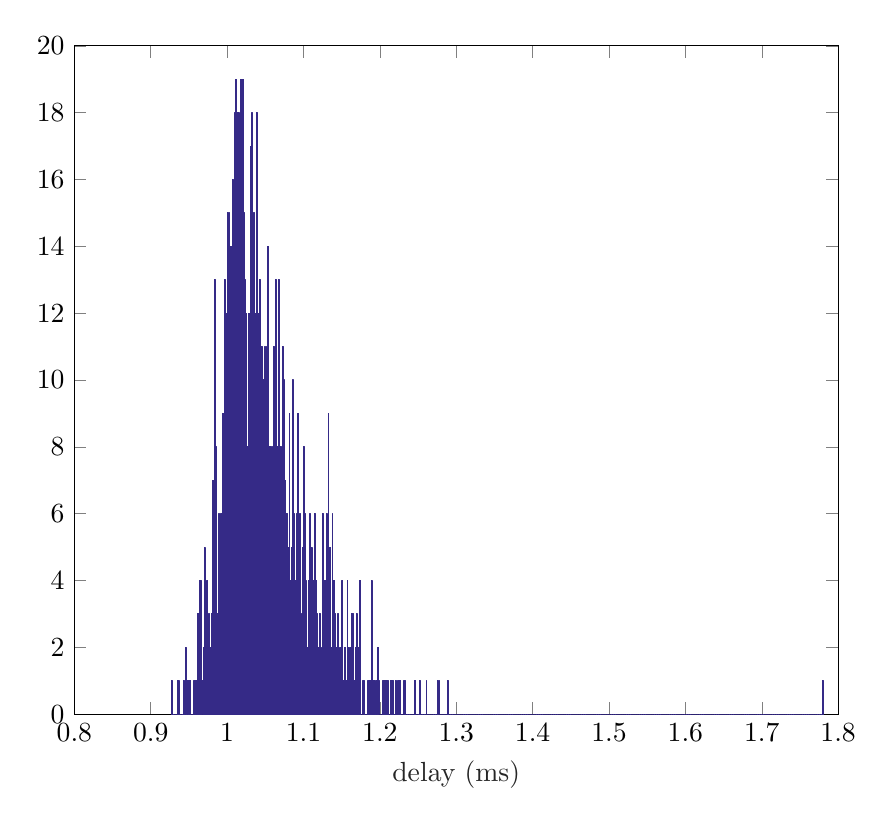
\begin{tikzpicture}

\begin{axis}[%
width=0.8\columnwidth,%7.484in,
height=0.7\columnwidth,%8.26in,
at={(0.745in,0.479in)},
scale only axis,
point meta min=1,
point meta max=2,
colormap={mymap}{[1pt] rgb(0pt)=(0.2081,0.1663,0.5292); rgb(1pt)=(0.211624,0.189781,0.577676); rgb(2pt)=(0.212252,0.213771,0.626971); rgb(3pt)=(0.2081,0.2386,0.677086); rgb(4pt)=(0.195905,0.264457,0.7279); rgb(5pt)=(0.170729,0.291938,0.779248); rgb(6pt)=(0.125271,0.324243,0.830271); rgb(7pt)=(0.0591333,0.359833,0.868333); rgb(8pt)=(0.0116952,0.38751,0.881957); rgb(9pt)=(0.00595714,0.408614,0.882843); rgb(10pt)=(0.0165143,0.4266,0.878633); rgb(11pt)=(0.0328524,0.443043,0.871957); rgb(12pt)=(0.0498143,0.458571,0.864057); rgb(13pt)=(0.0629333,0.47369,0.855438); rgb(14pt)=(0.0722667,0.488667,0.8467); rgb(15pt)=(0.0779429,0.503986,0.838371); rgb(16pt)=(0.0793476,0.520024,0.831181); rgb(17pt)=(0.0749429,0.537543,0.826271); rgb(18pt)=(0.0640571,0.556986,0.823957); rgb(19pt)=(0.0487714,0.577224,0.822829); rgb(20pt)=(0.0343429,0.596581,0.819852); rgb(21pt)=(0.0265,0.6137,0.8135); rgb(22pt)=(0.0238905,0.628662,0.803762); rgb(23pt)=(0.0230905,0.641786,0.791267); rgb(24pt)=(0.0227714,0.653486,0.776757); rgb(25pt)=(0.0266619,0.664195,0.760719); rgb(26pt)=(0.0383714,0.674271,0.743552); rgb(27pt)=(0.0589714,0.683757,0.725386); rgb(28pt)=(0.0843,0.692833,0.706167); rgb(29pt)=(0.113295,0.7015,0.685857); rgb(30pt)=(0.145271,0.709757,0.664629); rgb(31pt)=(0.180133,0.717657,0.642433); rgb(32pt)=(0.217829,0.725043,0.619262); rgb(33pt)=(0.258643,0.731714,0.595429); rgb(34pt)=(0.302171,0.737605,0.571186); rgb(35pt)=(0.348167,0.742433,0.547267); rgb(36pt)=(0.395257,0.7459,0.524443); rgb(37pt)=(0.44201,0.748081,0.503314); rgb(38pt)=(0.487124,0.749062,0.483976); rgb(39pt)=(0.530029,0.749114,0.466114); rgb(40pt)=(0.570857,0.748519,0.44939); rgb(41pt)=(0.609852,0.747314,0.433686); rgb(42pt)=(0.6473,0.7456,0.4188); rgb(43pt)=(0.683419,0.743476,0.404433); rgb(44pt)=(0.71841,0.741133,0.390476); rgb(45pt)=(0.752486,0.7384,0.376814); rgb(46pt)=(0.785843,0.735567,0.363271); rgb(47pt)=(0.818505,0.732733,0.34979); rgb(48pt)=(0.850657,0.7299,0.336029); rgb(49pt)=(0.882433,0.727433,0.3217); rgb(50pt)=(0.913933,0.725786,0.306276); rgb(51pt)=(0.944957,0.726114,0.288643); rgb(52pt)=(0.973895,0.731395,0.266648); rgb(53pt)=(0.993771,0.745457,0.240348); rgb(54pt)=(0.999043,0.765314,0.216414); rgb(55pt)=(0.995533,0.786057,0.196652); rgb(56pt)=(0.988,0.8066,0.179367); rgb(57pt)=(0.978857,0.827143,0.163314); rgb(58pt)=(0.9697,0.848138,0.147452); rgb(59pt)=(0.962586,0.870514,0.1309); rgb(60pt)=(0.958871,0.8949,0.113243); rgb(61pt)=(0.959824,0.921833,0.0948381); rgb(62pt)=(0.9661,0.951443,0.0755333); rgb(63pt)=(0.9763,0.9831,0.0538)},
xmin=0.8,
xmax=1.8,
xlabel style={font=\color{white!15!black}},
xlabel={delay (ms)},
ymin=0,
ymax=20,
axis background/.style={fill=white}
]

\addplot[area legend, table/row sep=crcr, patch, patch type=rectangle, shader=flat corner, forget plot, patch table with point meta={%
1	2	3	4	1\\
6	7	8	9	1\\
11	12	13	14	1\\
16	17	18	19	1\\
21	22	23	24	1\\
26	27	28	29	1\\
31	32	33	34	1\\
36	37	38	39	1\\
41	42	43	44	1\\
46	47	48	49	1\\
51	52	53	54	1\\
56	57	58	59	1\\
61	62	63	64	1\\
66	67	68	69	1\\
71	72	73	74	1\\
76	77	78	79	1\\
81	82	83	84	1\\
86	87	88	89	1\\
91	92	93	94	1\\
96	97	98	99	1\\
101	102	103	104	1\\
106	107	108	109	1\\
111	112	113	114	1\\
116	117	118	119	1\\
121	122	123	124	1\\
126	127	128	129	1\\
131	132	133	134	1\\
136	137	138	139	1\\
141	142	143	144	1\\
146	147	148	149	1\\
151	152	153	154	1\\
156	157	158	159	1\\
161	162	163	164	1\\
166	167	168	169	1\\
171	172	173	174	1\\
176	177	178	179	1\\
181	182	183	184	1\\
186	187	188	189	1\\
191	192	193	194	1\\
196	197	198	199	1\\
201	202	203	204	1\\
206	207	208	209	1\\
211	212	213	214	1\\
216	217	218	219	1\\
221	222	223	224	1\\
226	227	228	229	1\\
231	232	233	234	1\\
236	237	238	239	1\\
241	242	243	244	1\\
246	247	248	249	1\\
251	252	253	254	1\\
256	257	258	259	1\\
261	262	263	264	1\\
266	267	268	269	1\\
271	272	273	274	1\\
276	277	278	279	1\\
281	282	283	284	1\\
286	287	288	289	1\\
291	292	293	294	1\\
296	297	298	299	1\\
301	302	303	304	1\\
306	307	308	309	1\\
311	312	313	314	1\\
316	317	318	319	1\\
321	322	323	324	1\\
326	327	328	329	1\\
331	332	333	334	1\\
336	337	338	339	1\\
341	342	343	344	1\\
346	347	348	349	1\\
351	352	353	354	1\\
356	357	358	359	1\\
361	362	363	364	1\\
366	367	368	369	1\\
371	372	373	374	1\\
376	377	378	379	1\\
381	382	383	384	1\\
386	387	388	389	1\\
391	392	393	394	1\\
396	397	398	399	1\\
401	402	403	404	1\\
406	407	408	409	1\\
411	412	413	414	1\\
416	417	418	419	1\\
421	422	423	424	1\\
426	427	428	429	1\\
431	432	433	434	1\\
436	437	438	439	1\\
441	442	443	444	1\\
446	447	448	449	1\\
451	452	453	454	1\\
456	457	458	459	1\\
461	462	463	464	1\\
466	467	468	469	1\\
471	472	473	474	1\\
476	477	478	479	1\\
481	482	483	484	1\\
486	487	488	489	1\\
491	492	493	494	1\\
496	497	498	499	1\\
501	502	503	504	1\\
506	507	508	509	1\\
511	512	513	514	1\\
516	517	518	519	1\\
521	522	523	524	1\\
526	527	528	529	1\\
531	532	533	534	1\\
536	537	538	539	1\\
541	542	543	544	1\\
546	547	548	549	1\\
551	552	553	554	1\\
556	557	558	559	1\\
561	562	563	564	1\\
566	567	568	569	1\\
571	572	573	574	1\\
576	577	578	579	1\\
581	582	583	584	1\\
586	587	588	589	1\\
591	592	593	594	1\\
596	597	598	599	1\\
601	602	603	604	1\\
606	607	608	609	1\\
611	612	613	614	1\\
616	617	618	619	1\\
621	622	623	624	1\\
626	627	628	629	1\\
631	632	633	634	1\\
636	637	638	639	1\\
641	642	643	644	1\\
646	647	648	649	1\\
651	652	653	654	1\\
656	657	658	659	1\\
661	662	663	664	1\\
666	667	668	669	1\\
671	672	673	674	1\\
676	677	678	679	1\\
681	682	683	684	1\\
686	687	688	689	1\\
691	692	693	694	1\\
696	697	698	699	1\\
701	702	703	704	1\\
706	707	708	709	1\\
711	712	713	714	1\\
716	717	718	719	1\\
721	722	723	724	1\\
726	727	728	729	1\\
731	732	733	734	1\\
736	737	738	739	1\\
741	742	743	744	1\\
746	747	748	749	1\\
751	752	753	754	1\\
756	757	758	759	1\\
761	762	763	764	1\\
766	767	768	769	1\\
771	772	773	774	1\\
776	777	778	779	1\\
781	782	783	784	1\\
786	787	788	789	1\\
791	792	793	794	1\\
796	797	798	799	1\\
801	802	803	804	1\\
806	807	808	809	1\\
811	812	813	814	1\\
816	817	818	819	1\\
821	822	823	824	1\\
826	827	828	829	1\\
831	832	833	834	1\\
836	837	838	839	1\\
841	842	843	844	1\\
846	847	848	849	1\\
851	852	853	854	1\\
856	857	858	859	1\\
861	862	863	864	1\\
866	867	868	869	1\\
871	872	873	874	1\\
876	877	878	879	1\\
881	882	883	884	1\\
886	887	888	889	1\\
891	892	893	894	1\\
896	897	898	899	1\\
901	902	903	904	1\\
906	907	908	909	1\\
911	912	913	914	1\\
916	917	918	919	1\\
921	922	923	924	1\\
926	927	928	929	1\\
931	932	933	934	1\\
936	937	938	939	1\\
941	942	943	944	1\\
946	947	948	949	1\\
951	952	953	954	1\\
956	957	958	959	1\\
961	962	963	964	1\\
966	967	968	969	1\\
971	972	973	974	1\\
976	977	978	979	1\\
981	982	983	984	1\\
986	987	988	989	1\\
991	992	993	994	1\\
996	997	998	999	1\\
1001	1002	1003	1004	1\\
1006	1007	1008	1009	1\\
1011	1012	1013	1014	1\\
1016	1017	1018	1019	1\\
1021	1022	1023	1024	1\\
1026	1027	1028	1029	1\\
1031	1032	1033	1034	1\\
1036	1037	1038	1039	1\\
1041	1042	1043	1044	1\\
1046	1047	1048	1049	1\\
1051	1052	1053	1054	1\\
1056	1057	1058	1059	1\\
1061	1062	1063	1064	1\\
1066	1067	1068	1069	1\\
1071	1072	1073	1074	1\\
1076	1077	1078	1079	1\\
1081	1082	1083	1084	1\\
1086	1087	1088	1089	1\\
1091	1092	1093	1094	1\\
1096	1097	1098	1099	1\\
1101	1102	1103	1104	1\\
1106	1107	1108	1109	1\\
1111	1112	1113	1114	1\\
1116	1117	1118	1119	1\\
1121	1122	1123	1124	1\\
1126	1127	1128	1129	1\\
1131	1132	1133	1134	1\\
1136	1137	1138	1139	1\\
1141	1142	1143	1144	1\\
1146	1147	1148	1149	1\\
1151	1152	1153	1154	1\\
1156	1157	1158	1159	1\\
1161	1162	1163	1164	1\\
1166	1167	1168	1169	1\\
1171	1172	1173	1174	1\\
1176	1177	1178	1179	1\\
1181	1182	1183	1184	1\\
1186	1187	1188	1189	1\\
1191	1192	1193	1194	1\\
1196	1197	1198	1199	1\\
1201	1202	1203	1204	1\\
1206	1207	1208	1209	1\\
1211	1212	1213	1214	1\\
1216	1217	1218	1219	1\\
1221	1222	1223	1224	1\\
1226	1227	1228	1229	1\\
1231	1232	1233	1234	1\\
1236	1237	1238	1239	1\\
1241	1242	1243	1244	1\\
1246	1247	1248	1249	1\\
1251	1252	1253	1254	1\\
1256	1257	1258	1259	1\\
1261	1262	1263	1264	1\\
1266	1267	1268	1269	1\\
1271	1272	1273	1274	1\\
1276	1277	1278	1279	1\\
1281	1282	1283	1284	1\\
1286	1287	1288	1289	1\\
1291	1292	1293	1294	1\\
1296	1297	1298	1299	1\\
1301	1302	1303	1304	1\\
1306	1307	1308	1309	1\\
1311	1312	1313	1314	1\\
1316	1317	1318	1319	1\\
1321	1322	1323	1324	1\\
1326	1327	1328	1329	1\\
1331	1332	1333	1334	1\\
1336	1337	1338	1339	1\\
1341	1342	1343	1344	1\\
1346	1347	1348	1349	1\\
1351	1352	1353	1354	1\\
1356	1357	1358	1359	1\\
1361	1362	1363	1364	1\\
1366	1367	1368	1369	1\\
1371	1372	1373	1374	1\\
1376	1377	1378	1379	1\\
1381	1382	1383	1384	1\\
1386	1387	1388	1389	1\\
1391	1392	1393	1394	1\\
1396	1397	1398	1399	1\\
1401	1402	1403	1404	1\\
1406	1407	1408	1409	1\\
1411	1412	1413	1414	1\\
1416	1417	1418	1419	1\\
1421	1422	1423	1424	1\\
1426	1427	1428	1429	1\\
1431	1432	1433	1434	1\\
1436	1437	1438	1439	1\\
1441	1442	1443	1444	1\\
1446	1447	1448	1449	1\\
1451	1452	1453	1454	1\\
1456	1457	1458	1459	1\\
1461	1462	1463	1464	1\\
1466	1467	1468	1469	1\\
1471	1472	1473	1474	1\\
1476	1477	1478	1479	1\\
1481	1482	1483	1484	1\\
1486	1487	1488	1489	1\\
1491	1492	1493	1494	1\\
1496	1497	1498	1499	1\\
1501	1502	1503	1504	1\\
1506	1507	1508	1509	1\\
1511	1512	1513	1514	1\\
1516	1517	1518	1519	1\\
1521	1522	1523	1524	1\\
1526	1527	1528	1529	1\\
1531	1532	1533	1534	1\\
1536	1537	1538	1539	1\\
1541	1542	1543	1544	1\\
1546	1547	1548	1549	1\\
1551	1552	1553	1554	1\\
1556	1557	1558	1559	1\\
1561	1562	1563	1564	1\\
1566	1567	1568	1569	1\\
1571	1572	1573	1574	1\\
1576	1577	1578	1579	1\\
1581	1582	1583	1584	1\\
1586	1587	1588	1589	1\\
1591	1592	1593	1594	1\\
1596	1597	1598	1599	1\\
1601	1602	1603	1604	1\\
1606	1607	1608	1609	1\\
1611	1612	1613	1614	1\\
1616	1617	1618	1619	1\\
1621	1622	1623	1624	1\\
1626	1627	1628	1629	1\\
1631	1632	1633	1634	1\\
1636	1637	1638	1639	1\\
1641	1642	1643	1644	1\\
1646	1647	1648	1649	1\\
1651	1652	1653	1654	1\\
1656	1657	1658	1659	1\\
1661	1662	1663	1664	1\\
1666	1667	1668	1669	1\\
1671	1672	1673	1674	1\\
1676	1677	1678	1679	1\\
1681	1682	1683	1684	1\\
1686	1687	1688	1689	1\\
1691	1692	1693	1694	1\\
1696	1697	1698	1699	1\\
1701	1702	1703	1704	1\\
1706	1707	1708	1709	1\\
1711	1712	1713	1714	1\\
1716	1717	1718	1719	1\\
1721	1722	1723	1724	1\\
1726	1727	1728	1729	1\\
1731	1732	1733	1734	1\\
1736	1737	1738	1739	1\\
1741	1742	1743	1744	1\\
1746	1747	1748	1749	1\\
1751	1752	1753	1754	1\\
1756	1757	1758	1759	1\\
1761	1762	1763	1764	1\\
1766	1767	1768	1769	1\\
1771	1772	1773	1774	1\\
1776	1777	1778	1779	1\\
1781	1782	1783	1784	1\\
1786	1787	1788	1789	1\\
1791	1792	1793	1794	1\\
1796	1797	1798	1799	1\\
1801	1802	1803	1804	1\\
1806	1807	1808	1809	1\\
1811	1812	1813	1814	1\\
1816	1817	1818	1819	1\\
1821	1822	1823	1824	1\\
1826	1827	1828	1829	1\\
1831	1832	1833	1834	1\\
1836	1837	1838	1839	1\\
1841	1842	1843	1844	1\\
1846	1847	1848	1849	1\\
1851	1852	1853	1854	1\\
1856	1857	1858	1859	1\\
1861	1862	1863	1864	1\\
1866	1867	1868	1869	1\\
1871	1872	1873	1874	1\\
1876	1877	1878	1879	1\\
1881	1882	1883	1884	1\\
1886	1887	1888	1889	1\\
1891	1892	1893	1894	1\\
1896	1897	1898	1899	1\\
1901	1902	1903	1904	1\\
1906	1907	1908	1909	1\\
1911	1912	1913	1914	1\\
1916	1917	1918	1919	1\\
1921	1922	1923	1924	1\\
1926	1927	1928	1929	1\\
1931	1932	1933	1934	1\\
1936	1937	1938	1939	1\\
1941	1942	1943	1944	1\\
1946	1947	1948	1949	1\\
1951	1952	1953	1954	1\\
1956	1957	1958	1959	1\\
1961	1962	1963	1964	1\\
1966	1967	1968	1969	1\\
1971	1972	1973	1974	1\\
1976	1977	1978	1979	1\\
1981	1982	1983	1984	1\\
1986	1987	1988	1989	1\\
1991	1992	1993	1994	1\\
1996	1997	1998	1999	1\\
2001	2002	2003	2004	1\\
2006	2007	2008	2009	1\\
2011	2012	2013	2014	1\\
2016	2017	2018	2019	1\\
2021	2022	2023	2024	1\\
2026	2027	2028	2029	1\\
2031	2032	2033	2034	1\\
2036	2037	2038	2039	1\\
2041	2042	2043	2044	1\\
2046	2047	2048	2049	1\\
2051	2052	2053	2054	1\\
2056	2057	2058	2059	1\\
2061	2062	2063	2064	1\\
2066	2067	2068	2069	1\\
2071	2072	2073	2074	1\\
2076	2077	2078	2079	1\\
2081	2082	2083	2084	1\\
2086	2087	2088	2089	1\\
2091	2092	2093	2094	1\\
2096	2097	2098	2099	1\\
2101	2102	2103	2104	1\\
2106	2107	2108	2109	1\\
2111	2112	2113	2114	1\\
2116	2117	2118	2119	1\\
2121	2122	2123	2124	1\\
2126	2127	2128	2129	1\\
2131	2132	2133	2134	1\\
2136	2137	2138	2139	1\\
2141	2142	2143	2144	1\\
2146	2147	2148	2149	1\\
2151	2152	2153	2154	1\\
2156	2157	2158	2159	1\\
2161	2162	2163	2164	1\\
2166	2167	2168	2169	1\\
2171	2172	2173	2174	1\\
2176	2177	2178	2179	1\\
2181	2182	2183	2184	1\\
2186	2187	2188	2189	1\\
2191	2192	2193	2194	1\\
2196	2197	2198	2199	1\\
2201	2202	2203	2204	1\\
2206	2207	2208	2209	1\\
2211	2212	2213	2214	1\\
2216	2217	2218	2219	1\\
2221	2222	2223	2224	1\\
2226	2227	2228	2229	1\\
2231	2232	2233	2234	1\\
2236	2237	2238	2239	1\\
2241	2242	2243	2244	1\\
2246	2247	2248	2249	1\\
2251	2252	2253	2254	1\\
2256	2257	2258	2259	1\\
2261	2262	2263	2264	1\\
2266	2267	2268	2269	1\\
2271	2272	2273	2274	1\\
2276	2277	2278	2279	1\\
2281	2282	2283	2284	1\\
2286	2287	2288	2289	1\\
2291	2292	2293	2294	1\\
2296	2297	2298	2299	1\\
2301	2302	2303	2304	1\\
2306	2307	2308	2309	1\\
2311	2312	2313	2314	1\\
2316	2317	2318	2319	1\\
2321	2322	2323	2324	1\\
2326	2327	2328	2329	1\\
2331	2332	2333	2334	1\\
2336	2337	2338	2339	1\\
2341	2342	2343	2344	1\\
2346	2347	2348	2349	1\\
2351	2352	2353	2354	1\\
2356	2357	2358	2359	1\\
2361	2362	2363	2364	1\\
2366	2367	2368	2369	1\\
2371	2372	2373	2374	1\\
2376	2377	2378	2379	1\\
2381	2382	2383	2384	1\\
2386	2387	2388	2389	1\\
2391	2392	2393	2394	1\\
2396	2397	2398	2399	1\\
2401	2402	2403	2404	1\\
2406	2407	2408	2409	1\\
2411	2412	2413	2414	1\\
2416	2417	2418	2419	1\\
2421	2422	2423	2424	1\\
2426	2427	2428	2429	1\\
2431	2432	2433	2434	1\\
2436	2437	2438	2439	1\\
2441	2442	2443	2444	1\\
2446	2447	2448	2449	1\\
2451	2452	2453	2454	1\\
2456	2457	2458	2459	1\\
2461	2462	2463	2464	1\\
2466	2467	2468	2469	1\\
2471	2472	2473	2474	1\\
2476	2477	2478	2479	1\\
2481	2482	2483	2484	1\\
2486	2487	2488	2489	1\\
2491	2492	2493	2494	1\\
2496	2497	2498	2499	1\\
2501	2502	2503	2504	1\\
2506	2507	2508	2509	1\\
2511	2512	2513	2514	1\\
2516	2517	2518	2519	1\\
2521	2522	2523	2524	1\\
2526	2527	2528	2529	1\\
2531	2532	2533	2534	1\\
2536	2537	2538	2539	1\\
2541	2542	2543	2544	1\\
2546	2547	2548	2549	1\\
2551	2552	2553	2554	1\\
2556	2557	2558	2559	1\\
2561	2562	2563	2564	1\\
2566	2567	2568	2569	1\\
2571	2572	2573	2574	1\\
2576	2577	2578	2579	1\\
2581	2582	2583	2584	1\\
2586	2587	2588	2589	1\\
2591	2592	2593	2594	1\\
2596	2597	2598	2599	1\\
2601	2602	2603	2604	1\\
2606	2607	2608	2609	1\\
2611	2612	2613	2614	1\\
2616	2617	2618	2619	1\\
2621	2622	2623	2624	1\\
2626	2627	2628	2629	1\\
2631	2632	2633	2634	1\\
2636	2637	2638	2639	1\\
2641	2642	2643	2644	1\\
2646	2647	2648	2649	1\\
2651	2652	2653	2654	1\\
2656	2657	2658	2659	1\\
2661	2662	2663	2664	1\\
2666	2667	2668	2669	1\\
2671	2672	2673	2674	1\\
2676	2677	2678	2679	1\\
2681	2682	2683	2684	1\\
2686	2687	2688	2689	1\\
2691	2692	2693	2694	1\\
2696	2697	2698	2699	1\\
2701	2702	2703	2704	1\\
2706	2707	2708	2709	1\\
2711	2712	2713	2714	1\\
2716	2717	2718	2719	1\\
2721	2722	2723	2724	1\\
2726	2727	2728	2729	1\\
2731	2732	2733	2734	1\\
2736	2737	2738	2739	1\\
2741	2742	2743	2744	1\\
2746	2747	2748	2749	1\\
2751	2752	2753	2754	1\\
2756	2757	2758	2759	1\\
2761	2762	2763	2764	1\\
2766	2767	2768	2769	1\\
2771	2772	2773	2774	1\\
2776	2777	2778	2779	1\\
2781	2782	2783	2784	1\\
2786	2787	2788	2789	1\\
2791	2792	2793	2794	1\\
2796	2797	2798	2799	1\\
2801	2802	2803	2804	1\\
2806	2807	2808	2809	1\\
2811	2812	2813	2814	1\\
2816	2817	2818	2819	1\\
2821	2822	2823	2824	1\\
2826	2827	2828	2829	1\\
2831	2832	2833	2834	1\\
2836	2837	2838	2839	1\\
2841	2842	2843	2844	1\\
2846	2847	2848	2849	1\\
2851	2852	2853	2854	1\\
2856	2857	2858	2859	1\\
2861	2862	2863	2864	1\\
2866	2867	2868	2869	1\\
2871	2872	2873	2874	1\\
2876	2877	2878	2879	1\\
2881	2882	2883	2884	1\\
2886	2887	2888	2889	1\\
2891	2892	2893	2894	1\\
2896	2897	2898	2899	1\\
2901	2902	2903	2904	1\\
2906	2907	2908	2909	1\\
2911	2912	2913	2914	1\\
2916	2917	2918	2919	1\\
2921	2922	2923	2924	1\\
2926	2927	2928	2929	1\\
2931	2932	2933	2934	1\\
2936	2937	2938	2939	1\\
2941	2942	2943	2944	1\\
2946	2947	2948	2949	1\\
2951	2952	2953	2954	1\\
2956	2957	2958	2959	1\\
2961	2962	2963	2964	1\\
2966	2967	2968	2969	1\\
2971	2972	2973	2974	1\\
2976	2977	2978	2979	1\\
2981	2982	2983	2984	1\\
2986	2987	2988	2989	1\\
2991	2992	2993	2994	1\\
2996	2997	2998	2999	1\\
3001	3002	3003	3004	1\\
3006	3007	3008	3009	1\\
3011	3012	3013	3014	1\\
3016	3017	3018	3019	1\\
3021	3022	3023	3024	1\\
3026	3027	3028	3029	1\\
3031	3032	3033	3034	1\\
3036	3037	3038	3039	1\\
3041	3042	3043	3044	1\\
3046	3047	3048	3049	1\\
3051	3052	3053	3054	1\\
3056	3057	3058	3059	1\\
3061	3062	3063	3064	1\\
3066	3067	3068	3069	1\\
3071	3072	3073	3074	1\\
3076	3077	3078	3079	1\\
3081	3082	3083	3084	1\\
3086	3087	3088	3089	1\\
3091	3092	3093	3094	1\\
3096	3097	3098	3099	1\\
3101	3102	3103	3104	1\\
3106	3107	3108	3109	1\\
3111	3112	3113	3114	1\\
3116	3117	3118	3119	1\\
3121	3122	3123	3124	1\\
3126	3127	3128	3129	1\\
3131	3132	3133	3134	1\\
3136	3137	3138	3139	1\\
3141	3142	3143	3144	1\\
3146	3147	3148	3149	1\\
3151	3152	3153	3154	1\\
3156	3157	3158	3159	1\\
3161	3162	3163	3164	1\\
3166	3167	3168	3169	1\\
3171	3172	3173	3174	1\\
3176	3177	3178	3179	1\\
3181	3182	3183	3184	1\\
3186	3187	3188	3189	1\\
3191	3192	3193	3194	1\\
3196	3197	3198	3199	1\\
3201	3202	3203	3204	1\\
3206	3207	3208	3209	1\\
3211	3212	3213	3214	1\\
3216	3217	3218	3219	1\\
3221	3222	3223	3224	1\\
3226	3227	3228	3229	1\\
3231	3232	3233	3234	1\\
3236	3237	3238	3239	1\\
3241	3242	3243	3244	1\\
3246	3247	3248	3249	1\\
3251	3252	3253	3254	1\\
3256	3257	3258	3259	1\\
3261	3262	3263	3264	1\\
3266	3267	3268	3269	1\\
3271	3272	3273	3274	1\\
3276	3277	3278	3279	1\\
3281	3282	3283	3284	1\\
3286	3287	3288	3289	1\\
3291	3292	3293	3294	1\\
3296	3297	3298	3299	1\\
3301	3302	3303	3304	1\\
3306	3307	3308	3309	1\\
3311	3312	3313	3314	1\\
3316	3317	3318	3319	1\\
3321	3322	3323	3324	1\\
3326	3327	3328	3329	1\\
3331	3332	3333	3334	1\\
3336	3337	3338	3339	1\\
3341	3342	3343	3344	1\\
3346	3347	3348	3349	1\\
3351	3352	3353	3354	1\\
3356	3357	3358	3359	1\\
3361	3362	3363	3364	1\\
3366	3367	3368	3369	1\\
3371	3372	3373	3374	1\\
3376	3377	3378	3379	1\\
3381	3382	3383	3384	1\\
3386	3387	3388	3389	1\\
3391	3392	3393	3394	1\\
3396	3397	3398	3399	1\\
3401	3402	3403	3404	1\\
3406	3407	3408	3409	1\\
3411	3412	3413	3414	1\\
3416	3417	3418	3419	1\\
3421	3422	3423	3424	1\\
3426	3427	3428	3429	1\\
3431	3432	3433	3434	1\\
3436	3437	3438	3439	1\\
3441	3442	3443	3444	1\\
3446	3447	3448	3449	1\\
3451	3452	3453	3454	1\\
3456	3457	3458	3459	1\\
3461	3462	3463	3464	1\\
3466	3467	3468	3469	1\\
3471	3472	3473	3474	1\\
3476	3477	3478	3479	1\\
3481	3482	3483	3484	1\\
3486	3487	3488	3489	1\\
3491	3492	3493	3494	1\\
3496	3497	3498	3499	1\\
3501	3502	3503	3504	1\\
3506	3507	3508	3509	1\\
3511	3512	3513	3514	1\\
3516	3517	3518	3519	1\\
3521	3522	3523	3524	1\\
3526	3527	3528	3529	1\\
3531	3532	3533	3534	1\\
3536	3537	3538	3539	1\\
3541	3542	3543	3544	1\\
3546	3547	3548	3549	1\\
3551	3552	3553	3554	1\\
3556	3557	3558	3559	1\\
3561	3562	3563	3564	1\\
3566	3567	3568	3569	1\\
3571	3572	3573	3574	1\\
3576	3577	3578	3579	1\\
3581	3582	3583	3584	1\\
3586	3587	3588	3589	1\\
3591	3592	3593	3594	1\\
3596	3597	3598	3599	1\\
3601	3602	3603	3604	1\\
3606	3607	3608	3609	1\\
3611	3612	3613	3614	1\\
3616	3617	3618	3619	1\\
3621	3622	3623	3624	1\\
3626	3627	3628	3629	1\\
3631	3632	3633	3634	1\\
3636	3637	3638	3639	1\\
3641	3642	3643	3644	1\\
3646	3647	3648	3649	1\\
3651	3652	3653	3654	1\\
3656	3657	3658	3659	1\\
3661	3662	3663	3664	1\\
3666	3667	3668	3669	1\\
3671	3672	3673	3674	1\\
3676	3677	3678	3679	1\\
3681	3682	3683	3684	1\\
3686	3687	3688	3689	1\\
3691	3692	3693	3694	1\\
3696	3697	3698	3699	1\\
3701	3702	3703	3704	1\\
3706	3707	3708	3709	1\\
3711	3712	3713	3714	1\\
3716	3717	3718	3719	1\\
3721	3722	3723	3724	1\\
3726	3727	3728	3729	1\\
3731	3732	3733	3734	1\\
3736	3737	3738	3739	1\\
3741	3742	3743	3744	1\\
3746	3747	3748	3749	1\\
3751	3752	3753	3754	1\\
3756	3757	3758	3759	1\\
3761	3762	3763	3764	1\\
3766	3767	3768	3769	1\\
3771	3772	3773	3774	1\\
3776	3777	3778	3779	1\\
3781	3782	3783	3784	1\\
3786	3787	3788	3789	1\\
3791	3792	3793	3794	1\\
3796	3797	3798	3799	1\\
3801	3802	3803	3804	1\\
3806	3807	3808	3809	1\\
3811	3812	3813	3814	1\\
3816	3817	3818	3819	1\\
3821	3822	3823	3824	1\\
3826	3827	3828	3829	1\\
3831	3832	3833	3834	1\\
3836	3837	3838	3839	1\\
3841	3842	3843	3844	1\\
3846	3847	3848	3849	1\\
3851	3852	3853	3854	1\\
3856	3857	3858	3859	1\\
3861	3862	3863	3864	1\\
3866	3867	3868	3869	1\\
3871	3872	3873	3874	1\\
3876	3877	3878	3879	1\\
3881	3882	3883	3884	1\\
3886	3887	3888	3889	1\\
3891	3892	3893	3894	1\\
3896	3897	3898	3899	1\\
3901	3902	3903	3904	1\\
3906	3907	3908	3909	1\\
3911	3912	3913	3914	1\\
3916	3917	3918	3919	1\\
3921	3922	3923	3924	1\\
3926	3927	3928	3929	1\\
3931	3932	3933	3934	1\\
3936	3937	3938	3939	1\\
3941	3942	3943	3944	1\\
3946	3947	3948	3949	1\\
3951	3952	3953	3954	1\\
3956	3957	3958	3959	1\\
3961	3962	3963	3964	1\\
3966	3967	3968	3969	1\\
3971	3972	3973	3974	1\\
3976	3977	3978	3979	1\\
3981	3982	3983	3984	1\\
3986	3987	3988	3989	1\\
3991	3992	3993	3994	1\\
3996	3997	3998	3999	1\\
4001	4002	4003	4004	1\\
4006	4007	4008	4009	1\\
4011	4012	4013	4014	1\\
4016	4017	4018	4019	1\\
4021	4022	4023	4024	1\\
4026	4027	4028	4029	1\\
4031	4032	4033	4034	1\\
4036	4037	4038	4039	1\\
4041	4042	4043	4044	1\\
4046	4047	4048	4049	1\\
4051	4052	4053	4054	1\\
4056	4057	4058	4059	1\\
4061	4062	4063	4064	1\\
4066	4067	4068	4069	1\\
4071	4072	4073	4074	1\\
4076	4077	4078	4079	1\\
4081	4082	4083	4084	1\\
4086	4087	4088	4089	1\\
4091	4092	4093	4094	1\\
4096	4097	4098	4099	1\\
4101	4102	4103	4104	1\\
4106	4107	4108	4109	1\\
4111	4112	4113	4114	1\\
4116	4117	4118	4119	1\\
4121	4122	4123	4124	1\\
4126	4127	4128	4129	1\\
4131	4132	4133	4134	1\\
4136	4137	4138	4139	1\\
4141	4142	4143	4144	1\\
4146	4147	4148	4149	1\\
4151	4152	4153	4154	1\\
4156	4157	4158	4159	1\\
4161	4162	4163	4164	1\\
4166	4167	4168	4169	1\\
4171	4172	4173	4174	1\\
4176	4177	4178	4179	1\\
4181	4182	4183	4184	1\\
4186	4187	4188	4189	1\\
4191	4192	4193	4194	1\\
4196	4197	4198	4199	1\\
4201	4202	4203	4204	1\\
4206	4207	4208	4209	1\\
4211	4212	4213	4214	1\\
4216	4217	4218	4219	1\\
4221	4222	4223	4224	1\\
4226	4227	4228	4229	1\\
4231	4232	4233	4234	1\\
4236	4237	4238	4239	1\\
4241	4242	4243	4244	1\\
4246	4247	4248	4249	1\\
4251	4252	4253	4254	1\\
4256	4257	4258	4259	1\\
4261	4262	4263	4264	1\\
4266	4267	4268	4269	1\\
4271	4272	4273	4274	1\\
4276	4277	4278	4279	1\\
4281	4282	4283	4284	1\\
4286	4287	4288	4289	1\\
4291	4292	4293	4294	1\\
4296	4297	4298	4299	1\\
4301	4302	4303	4304	1\\
4306	4307	4308	4309	1\\
4311	4312	4313	4314	1\\
4316	4317	4318	4319	1\\
4321	4322	4323	4324	1\\
4326	4327	4328	4329	1\\
4331	4332	4333	4334	1\\
4336	4337	4338	4339	1\\
4341	4342	4343	4344	1\\
4346	4347	4348	4349	1\\
4351	4352	4353	4354	1\\
4356	4357	4358	4359	1\\
4361	4362	4363	4364	1\\
4366	4367	4368	4369	1\\
4371	4372	4373	4374	1\\
4376	4377	4378	4379	1\\
4381	4382	4383	4384	1\\
4386	4387	4388	4389	1\\
4391	4392	4393	4394	1\\
4396	4397	4398	4399	1\\
4401	4402	4403	4404	1\\
4406	4407	4408	4409	1\\
4411	4412	4413	4414	1\\
4416	4417	4418	4419	1\\
4421	4422	4423	4424	1\\
4426	4427	4428	4429	1\\
4431	4432	4433	4434	1\\
4436	4437	4438	4439	1\\
4441	4442	4443	4444	1\\
4446	4447	4448	4449	1\\
4451	4452	4453	4454	1\\
4456	4457	4458	4459	1\\
4461	4462	4463	4464	1\\
4466	4467	4468	4469	1\\
4471	4472	4473	4474	1\\
4476	4477	4478	4479	1\\
4481	4482	4483	4484	1\\
4486	4487	4488	4489	1\\
4491	4492	4493	4494	1\\
4496	4497	4498	4499	1\\
4501	4502	4503	4504	1\\
4506	4507	4508	4509	1\\
4511	4512	4513	4514	1\\
4516	4517	4518	4519	1\\
4521	4522	4523	4524	1\\
4526	4527	4528	4529	1\\
4531	4532	4533	4534	1\\
4536	4537	4538	4539	1\\
4541	4542	4543	4544	1\\
4546	4547	4548	4549	1\\
4551	4552	4553	4554	1\\
4556	4557	4558	4559	1\\
4561	4562	4563	4564	1\\
4566	4567	4568	4569	1\\
4571	4572	4573	4574	1\\
4576	4577	4578	4579	1\\
4581	4582	4583	4584	1\\
4586	4587	4588	4589	1\\
4591	4592	4593	4594	1\\
4596	4597	4598	4599	1\\
4601	4602	4603	4604	1\\
4606	4607	4608	4609	1\\
4611	4612	4613	4614	1\\
4616	4617	4618	4619	1\\
4621	4622	4623	4624	1\\
4626	4627	4628	4629	1\\
4631	4632	4633	4634	1\\
4636	4637	4638	4639	1\\
4641	4642	4643	4644	1\\
4646	4647	4648	4649	1\\
4651	4652	4653	4654	1\\
4656	4657	4658	4659	1\\
4661	4662	4663	4664	1\\
4666	4667	4668	4669	1\\
4671	4672	4673	4674	1\\
4676	4677	4678	4679	1\\
4681	4682	4683	4684	1\\
4686	4687	4688	4689	1\\
4691	4692	4693	4694	1\\
4696	4697	4698	4699	1\\
4701	4702	4703	4704	1\\
4706	4707	4708	4709	1\\
4711	4712	4713	4714	1\\
4716	4717	4718	4719	1\\
4721	4722	4723	4724	1\\
4726	4727	4728	4729	1\\
4731	4732	4733	4734	1\\
4736	4737	4738	4739	1\\
4741	4742	4743	4744	1\\
4746	4747	4748	4749	1\\
4751	4752	4753	4754	1\\
4756	4757	4758	4759	1\\
4761	4762	4763	4764	1\\
4766	4767	4768	4769	1\\
4771	4772	4773	4774	1\\
4776	4777	4778	4779	1\\
4781	4782	4783	4784	1\\
4786	4787	4788	4789	1\\
4791	4792	4793	4794	1\\
4796	4797	4798	4799	1\\
4801	4802	4803	4804	1\\
4806	4807	4808	4809	1\\
4811	4812	4813	4814	1\\
4816	4817	4818	4819	1\\
4821	4822	4823	4824	1\\
4826	4827	4828	4829	1\\
4831	4832	4833	4834	1\\
4836	4837	4838	4839	1\\
4841	4842	4843	4844	1\\
4846	4847	4848	4849	1\\
4851	4852	4853	4854	1\\
4856	4857	4858	4859	1\\
4861	4862	4863	4864	1\\
4866	4867	4868	4869	1\\
4871	4872	4873	4874	1\\
4876	4877	4878	4879	1\\
4881	4882	4883	4884	1\\
4886	4887	4888	4889	1\\
4891	4892	4893	4894	1\\
4896	4897	4898	4899	1\\
4901	4902	4903	4904	1\\
4906	4907	4908	4909	1\\
4911	4912	4913	4914	1\\
4916	4917	4918	4919	1\\
4921	4922	4923	4924	1\\
4926	4927	4928	4929	1\\
4931	4932	4933	4934	1\\
4936	4937	4938	4939	1\\
4941	4942	4943	4944	1\\
4946	4947	4948	4949	1\\
4951	4952	4953	4954	1\\
4956	4957	4958	4959	1\\
4961	4962	4963	4964	1\\
4966	4967	4968	4969	1\\
4971	4972	4973	4974	1\\
4976	4977	4978	4979	1\\
4981	4982	4983	4984	1\\
4986	4987	4988	4989	1\\
4991	4992	4993	4994	1\\
4996	4997	4998	4999	1\\
}]
table[row sep=crcr] {%
x	y\\
0.926733016967773	0\\
0.926733016967773	0\\
0.926733016967773	1\\
0.927586555480957	1\\
0.927586555480957	0\\
0.927586555480957	0\\
0.927586555480957	0\\
0.927586555480957	1\\
0.928440093994141	1\\
0.928440093994141	0\\
0.928440093994141	0\\
0.928440093994141	0\\
0.928440093994141	0\\
0.929293632507324	0\\
0.929293632507324	0\\
0.929293632507324	0\\
0.929293632507324	0\\
0.929293632507324	0\\
0.930147171020508	0\\
0.930147171020508	0\\
0.930147171020508	0\\
0.930147171020508	0\\
0.930147171020508	0\\
0.931000709533691	0\\
0.931000709533691	0\\
0.931000709533691	0\\
0.931000709533691	0\\
0.931000709533691	0\\
0.931854248046875	0\\
0.931854248046875	0\\
0.931854248046875	0\\
0.931854248046875	0\\
0.931854248046875	0\\
0.932707786560059	0\\
0.932707786560059	0\\
0.932707786560059	0\\
0.932707786560059	0\\
0.932707786560059	0\\
0.933561325073242	0\\
0.933561325073242	0\\
0.933561325073242	0\\
0.933561325073242	0\\
0.933561325073242	0\\
0.934414863586426	0\\
0.934414863586426	0\\
0.934414863586426	0\\
0.934414863586426	0\\
0.934414863586426	0\\
0.935268402099609	0\\
0.935268402099609	0\\
0.935268402099609	0\\
0.935268402099609	0\\
0.935268402099609	1\\
0.936121940612793	1\\
0.936121940612793	0\\
0.936121940612793	0\\
0.936121940612793	0\\
0.936121940612793	1\\
0.936975479125977	1\\
0.936975479125977	0\\
0.936975479125977	0\\
0.936975479125977	0\\
0.936975479125977	0\\
0.93782901763916	0\\
0.93782901763916	0\\
0.93782901763916	0\\
0.93782901763916	0\\
0.93782901763916	0\\
0.938682556152344	0\\
0.938682556152344	0\\
0.938682556152344	0\\
0.938682556152344	0\\
0.938682556152344	0\\
0.939536094665527	0\\
0.939536094665527	0\\
0.939536094665527	0\\
0.939536094665527	0\\
0.939536094665527	0\\
0.940389633178711	0\\
0.940389633178711	0\\
0.940389633178711	0\\
0.940389633178711	0\\
0.940389633178711	0\\
0.941243171691895	0\\
0.941243171691895	0\\
0.941243171691895	0\\
0.941243171691895	0\\
0.941243171691895	0\\
0.942096710205078	0\\
0.942096710205078	0\\
0.942096710205078	0\\
0.942096710205078	0\\
0.942096710205078	0\\
0.942950248718262	0\\
0.942950248718262	0\\
0.942950248718262	0\\
0.942950248718262	0\\
0.942950248718262	1\\
0.943803787231445	1\\
0.943803787231445	0\\
0.943803787231445	0\\
0.943803787231445	0\\
0.943803787231445	0\\
0.944657325744629	0\\
0.944657325744629	0\\
0.944657325744629	0\\
0.944657325744629	0\\
0.944657325744629	0\\
0.945510864257812	0\\
0.945510864257812	0\\
0.945510864257812	0\\
0.945510864257812	0\\
0.945510864257812	2\\
0.946364402770996	2\\
0.946364402770996	0\\
0.946364402770996	0\\
0.946364402770996	0\\
0.946364402770996	0\\
0.94721794128418	0\\
0.94721794128418	0\\
0.94721794128418	0\\
0.94721794128418	0\\
0.94721794128418	0\\
0.948071479797363	0\\
0.948071479797363	0\\
0.948071479797363	0\\
0.948071479797363	0\\
0.948071479797363	1\\
0.948925018310547	1\\
0.948925018310547	0\\
0.948925018310547	0\\
0.948925018310547	0\\
0.948925018310547	0\\
0.94977855682373	0\\
0.94977855682373	0\\
0.94977855682373	0\\
0.94977855682373	0\\
0.94977855682373	1\\
0.950632095336914	1\\
0.950632095336914	0\\
0.950632095336914	0\\
0.950632095336914	0\\
0.950632095336914	1\\
0.951485633850098	1\\
0.951485633850098	0\\
0.951485633850098	0\\
0.951485633850098	0\\
0.951485633850098	1\\
0.952339172363281	1\\
0.952339172363281	0\\
0.952339172363281	0\\
0.952339172363281	0\\
0.952339172363281	0\\
0.953192710876465	0\\
0.953192710876465	0\\
0.953192710876465	0\\
0.953192710876465	0\\
0.953192710876465	0\\
0.954046249389648	0\\
0.954046249389648	0\\
0.954046249389648	0\\
0.954046249389648	0\\
0.954046249389648	0\\
0.954899787902832	0\\
0.954899787902832	0\\
0.954899787902832	0\\
0.954899787902832	0\\
0.954899787902832	0\\
0.955753326416016	0\\
0.955753326416016	0\\
0.955753326416016	0\\
0.955753326416016	0\\
0.955753326416016	0\\
0.956606864929199	0\\
0.956606864929199	0\\
0.956606864929199	0\\
0.956606864929199	0\\
0.956606864929199	1\\
0.957460403442383	1\\
0.957460403442383	0\\
0.957460403442383	0\\
0.957460403442383	0\\
0.957460403442383	1\\
0.958313941955566	1\\
0.958313941955566	0\\
0.958313941955566	0\\
0.958313941955566	0\\
0.958313941955566	1\\
0.95916748046875	1\\
0.95916748046875	0\\
0.95916748046875	0\\
0.95916748046875	0\\
0.95916748046875	0\\
0.960021018981934	0\\
0.960021018981934	0\\
0.960021018981934	0\\
0.960021018981934	0\\
0.960021018981934	1\\
0.960874557495117	1\\
0.960874557495117	0\\
0.960874557495117	0\\
0.960874557495117	0\\
0.960874557495117	1\\
0.961728096008301	1\\
0.961728096008301	0\\
0.961728096008301	0\\
0.961728096008301	0\\
0.961728096008301	3\\
0.962581634521484	3\\
0.962581634521484	0\\
0.962581634521484	0\\
0.962581634521484	0\\
0.962581634521484	3\\
0.963435173034668	3\\
0.963435173034668	0\\
0.963435173034668	0\\
0.963435173034668	0\\
0.963435173034668	0\\
0.964288711547852	0\\
0.964288711547852	0\\
0.964288711547852	0\\
0.964288711547852	0\\
0.964288711547852	4\\
0.965142250061035	4\\
0.965142250061035	0\\
0.965142250061035	0\\
0.965142250061035	0\\
0.965142250061035	4\\
0.965995788574219	4\\
0.965995788574219	0\\
0.965995788574219	0\\
0.965995788574219	0\\
0.965995788574219	1\\
0.966849327087402	1\\
0.966849327087402	0\\
0.966849327087402	0\\
0.966849327087402	0\\
0.966849327087402	0\\
0.967702865600586	0\\
0.967702865600586	0\\
0.967702865600586	0\\
0.967702865600586	0\\
0.967702865600586	1\\
0.96855640411377	1\\
0.96855640411377	0\\
0.96855640411377	0\\
0.96855640411377	0\\
0.96855640411377	0\\
0.969409942626953	0\\
0.969409942626953	0\\
0.969409942626953	0\\
0.969409942626953	0\\
0.969409942626953	2\\
0.970263481140137	2\\
0.970263481140137	0\\
0.970263481140137	0\\
0.970263481140137	0\\
0.970263481140137	5\\
0.97111701965332	5\\
0.97111701965332	0\\
0.97111701965332	0\\
0.97111701965332	0\\
0.97111701965332	1\\
0.971970558166504	1\\
0.971970558166504	0\\
0.971970558166504	0\\
0.971970558166504	0\\
0.971970558166504	0\\
0.972824096679688	0\\
0.972824096679688	0\\
0.972824096679688	0\\
0.972824096679688	0\\
0.972824096679688	3\\
0.973677635192871	3\\
0.973677635192871	0\\
0.973677635192871	0\\
0.973677635192871	0\\
0.973677635192871	4\\
0.974531173706055	4\\
0.974531173706055	0\\
0.974531173706055	0\\
0.974531173706055	0\\
0.974531173706055	2\\
0.975384712219238	2\\
0.975384712219238	0\\
0.975384712219238	0\\
0.975384712219238	0\\
0.975384712219238	1\\
0.976238250732422	1\\
0.976238250732422	0\\
0.976238250732422	0\\
0.976238250732422	0\\
0.976238250732422	3\\
0.977091789245605	3\\
0.977091789245605	0\\
0.977091789245605	0\\
0.977091789245605	0\\
0.977091789245605	2\\
0.977945327758789	2\\
0.977945327758789	0\\
0.977945327758789	0\\
0.977945327758789	0\\
0.977945327758789	1\\
0.978798866271973	1\\
0.978798866271973	0\\
0.978798866271973	0\\
0.978798866271973	0\\
0.978798866271973	1\\
0.979652404785156	1\\
0.979652404785156	0\\
0.979652404785156	0\\
0.979652404785156	0\\
0.979652404785156	3\\
0.98050594329834	3\\
0.98050594329834	0\\
0.98050594329834	0\\
0.98050594329834	0\\
0.98050594329834	6\\
0.981359481811523	6\\
0.981359481811523	0\\
0.981359481811523	0\\
0.981359481811523	0\\
0.981359481811523	7\\
0.982213020324707	7\\
0.982213020324707	0\\
0.982213020324707	0\\
0.982213020324707	0\\
0.982213020324707	5\\
0.983066558837891	5\\
0.983066558837891	0\\
0.983066558837891	0\\
0.983066558837891	0\\
0.983066558837891	4\\
0.983920097351074	4\\
0.983920097351074	0\\
0.983920097351074	0\\
0.983920097351074	0\\
0.983920097351074	13\\
0.984773635864258	13\\
0.984773635864258	0\\
0.984773635864258	0\\
0.984773635864258	0\\
0.984773635864258	8\\
0.985627174377441	8\\
0.985627174377441	0\\
0.985627174377441	0\\
0.985627174377441	0\\
0.985627174377441	4\\
0.986480712890625	4\\
0.986480712890625	0\\
0.986480712890625	0\\
0.986480712890625	0\\
0.986480712890625	1\\
0.987334251403809	1\\
0.987334251403809	0\\
0.987334251403809	0\\
0.987334251403809	0\\
0.987334251403809	3\\
0.988187789916992	3\\
0.988187789916992	0\\
0.988187789916992	0\\
0.988187789916992	0\\
0.988187789916992	6\\
0.989041328430176	6\\
0.989041328430176	0\\
0.989041328430176	0\\
0.989041328430176	0\\
0.989041328430176	5\\
0.989894866943359	5\\
0.989894866943359	0\\
0.989894866943359	0\\
0.989894866943359	0\\
0.989894866943359	5\\
0.990748405456543	5\\
0.990748405456543	0\\
0.990748405456543	0\\
0.990748405456543	0\\
0.990748405456543	6\\
0.991601943969727	6\\
0.991601943969727	0\\
0.991601943969727	0\\
0.991601943969727	0\\
0.991601943969727	5\\
0.99245548248291	5\\
0.99245548248291	0\\
0.99245548248291	0\\
0.99245548248291	0\\
0.99245548248291	6\\
0.993309020996094	6\\
0.993309020996094	0\\
0.993309020996094	0\\
0.993309020996094	0\\
0.993309020996094	5\\
0.994162559509277	5\\
0.994162559509277	0\\
0.994162559509277	0\\
0.994162559509277	0\\
0.994162559509277	9\\
0.995016098022461	9\\
0.995016098022461	0\\
0.995016098022461	0\\
0.995016098022461	0\\
0.995016098022461	9\\
0.995869636535645	9\\
0.995869636535645	0\\
0.995869636535645	0\\
0.995869636535645	0\\
0.995869636535645	4\\
0.996723175048828	4\\
0.996723175048828	0\\
0.996723175048828	0\\
0.996723175048828	0\\
0.996723175048828	13\\
0.997576713562012	13\\
0.997576713562012	0\\
0.997576713562012	0\\
0.997576713562012	0\\
0.997576713562012	8\\
0.998430252075195	8\\
0.998430252075195	0\\
0.998430252075195	0\\
0.998430252075195	0\\
0.998430252075195	9\\
0.999283790588379	9\\
0.999283790588379	0\\
0.999283790588379	0\\
0.999283790588379	0\\
0.999283790588379	12\\
1.00013732910156	12\\
1.00013732910156	0\\
1.00013732910156	0\\
1.00013732910156	0\\
1.00013732910156	15\\
1.00099086761475	15\\
1.00099086761475	0\\
1.00099086761475	0\\
1.00099086761475	0\\
1.00099086761475	15\\
1.00184440612793	15\\
1.00184440612793	0\\
1.00184440612793	0\\
1.00184440612793	0\\
1.00184440612793	12\\
1.00269794464111	12\\
1.00269794464111	0\\
1.00269794464111	0\\
1.00269794464111	0\\
1.00269794464111	15\\
1.0035514831543	15\\
1.0035514831543	0\\
1.0035514831543	0\\
1.0035514831543	0\\
1.0035514831543	7\\
1.00440502166748	7\\
1.00440502166748	0\\
1.00440502166748	0\\
1.00440502166748	0\\
1.00440502166748	14\\
1.00525856018066	14\\
1.00525856018066	0\\
1.00525856018066	0\\
1.00525856018066	0\\
1.00525856018066	4\\
1.00611209869385	4\\
1.00611209869385	0\\
1.00611209869385	0\\
1.00611209869385	0\\
1.00611209869385	14\\
1.00696563720703	14\\
1.00696563720703	0\\
1.00696563720703	0\\
1.00696563720703	0\\
1.00696563720703	16\\
1.00781917572021	16\\
1.00781917572021	0\\
1.00781917572021	0\\
1.00781917572021	0\\
1.00781917572021	4\\
1.0086727142334	4\\
1.0086727142334	0\\
1.0086727142334	0\\
1.0086727142334	0\\
1.0086727142334	13\\
1.00952625274658	13\\
1.00952625274658	0\\
1.00952625274658	0\\
1.00952625274658	0\\
1.00952625274658	8\\
1.01037979125977	8\\
1.01037979125977	0\\
1.01037979125977	0\\
1.01037979125977	0\\
1.01037979125977	18\\
1.01123332977295	18\\
1.01123332977295	0\\
1.01123332977295	0\\
1.01123332977295	0\\
1.01123332977295	19\\
1.01208686828613	19\\
1.01208686828613	0\\
1.01208686828613	0\\
1.01208686828613	0\\
1.01208686828613	10\\
1.01294040679932	10\\
1.01294040679932	0\\
1.01294040679932	0\\
1.01294040679932	0\\
1.01294040679932	11\\
1.0137939453125	11\\
1.0137939453125	0\\
1.0137939453125	0\\
1.0137939453125	0\\
1.0137939453125	18\\
1.01464748382568	18\\
1.01464748382568	0\\
1.01464748382568	0\\
1.01464748382568	0\\
1.01464748382568	18\\
1.01550102233887	18\\
1.01550102233887	0\\
1.01550102233887	0\\
1.01550102233887	0\\
1.01550102233887	10\\
1.01635456085205	10\\
1.01635456085205	0\\
1.01635456085205	0\\
1.01635456085205	0\\
1.01635456085205	13\\
1.01720809936523	13\\
1.01720809936523	0\\
1.01720809936523	0\\
1.01720809936523	0\\
1.01720809936523	19\\
1.01806163787842	19\\
1.01806163787842	0\\
1.01806163787842	0\\
1.01806163787842	0\\
1.01806163787842	9\\
1.0189151763916	9\\
1.0189151763916	0\\
1.0189151763916	0\\
1.0189151763916	0\\
1.0189151763916	19\\
1.01976871490479	19\\
1.01976871490479	0\\
1.01976871490479	0\\
1.01976871490479	0\\
1.01976871490479	10\\
1.02062225341797	10\\
1.02062225341797	0\\
1.02062225341797	0\\
1.02062225341797	0\\
1.02062225341797	19\\
1.02147579193115	19\\
1.02147579193115	0\\
1.02147579193115	0\\
1.02147579193115	0\\
1.02147579193115	12\\
1.02232933044434	12\\
1.02232933044434	0\\
1.02232933044434	0\\
1.02232933044434	0\\
1.02232933044434	15\\
1.02318286895752	15\\
1.02318286895752	0\\
1.02318286895752	0\\
1.02318286895752	0\\
1.02318286895752	13\\
1.0240364074707	13\\
1.0240364074707	0\\
1.0240364074707	0\\
1.0240364074707	0\\
1.0240364074707	8\\
1.02488994598389	8\\
1.02488994598389	0\\
1.02488994598389	0\\
1.02488994598389	0\\
1.02488994598389	12\\
1.02574348449707	12\\
1.02574348449707	0\\
1.02574348449707	0\\
1.02574348449707	0\\
1.02574348449707	5\\
1.02659702301025	5\\
1.02659702301025	0\\
1.02659702301025	0\\
1.02659702301025	0\\
1.02659702301025	8\\
1.02745056152344	8\\
1.02745056152344	0\\
1.02745056152344	0\\
1.02745056152344	0\\
1.02745056152344	12\\
1.02830410003662	12\\
1.02830410003662	0\\
1.02830410003662	0\\
1.02830410003662	0\\
1.02830410003662	12\\
1.0291576385498	12\\
1.0291576385498	0\\
1.0291576385498	0\\
1.0291576385498	0\\
1.0291576385498	8\\
1.03001117706299	8\\
1.03001117706299	0\\
1.03001117706299	0\\
1.03001117706299	0\\
1.03001117706299	6\\
1.03086471557617	6\\
1.03086471557617	0\\
1.03086471557617	0\\
1.03086471557617	0\\
1.03086471557617	17\\
1.03171825408936	17\\
1.03171825408936	0\\
1.03171825408936	0\\
1.03171825408936	0\\
1.03171825408936	13\\
1.03257179260254	13\\
1.03257179260254	0\\
1.03257179260254	0\\
1.03257179260254	0\\
1.03257179260254	18\\
1.03342533111572	18\\
1.03342533111572	0\\
1.03342533111572	0\\
1.03342533111572	0\\
1.03342533111572	5\\
1.03427886962891	5\\
1.03427886962891	0\\
1.03427886962891	0\\
1.03427886962891	0\\
1.03427886962891	11\\
1.03513240814209	11\\
1.03513240814209	0\\
1.03513240814209	0\\
1.03513240814209	0\\
1.03513240814209	15\\
1.03598594665527	15\\
1.03598594665527	0\\
1.03598594665527	0\\
1.03598594665527	0\\
1.03598594665527	12\\
1.03683948516846	12\\
1.03683948516846	0\\
1.03683948516846	0\\
1.03683948516846	0\\
1.03683948516846	10\\
1.03769302368164	10\\
1.03769302368164	0\\
1.03769302368164	0\\
1.03769302368164	0\\
1.03769302368164	8\\
1.03854656219482	8\\
1.03854656219482	0\\
1.03854656219482	0\\
1.03854656219482	0\\
1.03854656219482	18\\
1.03940010070801	18\\
1.03940010070801	0\\
1.03940010070801	0\\
1.03940010070801	0\\
1.03940010070801	13\\
1.04025363922119	13\\
1.04025363922119	0\\
1.04025363922119	0\\
1.04025363922119	0\\
1.04025363922119	12\\
1.04110717773438	12\\
1.04110717773438	0\\
1.04110717773438	0\\
1.04110717773438	0\\
1.04110717773438	7\\
1.04196071624756	7\\
1.04196071624756	0\\
1.04196071624756	0\\
1.04196071624756	0\\
1.04196071624756	6\\
1.04281425476074	6\\
1.04281425476074	0\\
1.04281425476074	0\\
1.04281425476074	0\\
1.04281425476074	13\\
1.04366779327393	13\\
1.04366779327393	0\\
1.04366779327393	0\\
1.04366779327393	0\\
1.04366779327393	8\\
1.04452133178711	8\\
1.04452133178711	0\\
1.04452133178711	0\\
1.04452133178711	0\\
1.04452133178711	8\\
1.04537487030029	8\\
1.04537487030029	0\\
1.04537487030029	0\\
1.04537487030029	0\\
1.04537487030029	11\\
1.04622840881348	11\\
1.04622840881348	0\\
1.04622840881348	0\\
1.04622840881348	0\\
1.04622840881348	7\\
1.04708194732666	7\\
1.04708194732666	0\\
1.04708194732666	0\\
1.04708194732666	0\\
1.04708194732666	10\\
1.04793548583984	10\\
1.04793548583984	0\\
1.04793548583984	0\\
1.04793548583984	0\\
1.04793548583984	10\\
1.04878902435303	10\\
1.04878902435303	0\\
1.04878902435303	0\\
1.04878902435303	0\\
1.04878902435303	8\\
1.04964256286621	8\\
1.04964256286621	0\\
1.04964256286621	0\\
1.04964256286621	0\\
1.04964256286621	11\\
1.05049610137939	11\\
1.05049610137939	0\\
1.05049610137939	0\\
1.05049610137939	0\\
1.05049610137939	8\\
1.05134963989258	8\\
1.05134963989258	0\\
1.05134963989258	0\\
1.05134963989258	0\\
1.05134963989258	4\\
1.05220317840576	4\\
1.05220317840576	0\\
1.05220317840576	0\\
1.05220317840576	0\\
1.05220317840576	11\\
1.05305671691895	11\\
1.05305671691895	0\\
1.05305671691895	0\\
1.05305671691895	0\\
1.05305671691895	14\\
1.05391025543213	14\\
1.05391025543213	0\\
1.05391025543213	0\\
1.05391025543213	0\\
1.05391025543213	8\\
1.05476379394531	8\\
1.05476379394531	0\\
1.05476379394531	0\\
1.05476379394531	0\\
1.05476379394531	4\\
1.0556173324585	4\\
1.0556173324585	0\\
1.0556173324585	0\\
1.0556173324585	0\\
1.0556173324585	8\\
1.05647087097168	8\\
1.05647087097168	0\\
1.05647087097168	0\\
1.05647087097168	0\\
1.05647087097168	2\\
1.05732440948486	2\\
1.05732440948486	0\\
1.05732440948486	0\\
1.05732440948486	0\\
1.05732440948486	8\\
1.05817794799805	8\\
1.05817794799805	0\\
1.05817794799805	0\\
1.05817794799805	0\\
1.05817794799805	7\\
1.05903148651123	7\\
1.05903148651123	0\\
1.05903148651123	0\\
1.05903148651123	0\\
1.05903148651123	8\\
1.05988502502441	8\\
1.05988502502441	0\\
1.05988502502441	0\\
1.05988502502441	0\\
1.05988502502441	1\\
1.0607385635376	1\\
1.0607385635376	0\\
1.0607385635376	0\\
1.0607385635376	0\\
1.0607385635376	11\\
1.06159210205078	11\\
1.06159210205078	0\\
1.06159210205078	0\\
1.06159210205078	0\\
1.06159210205078	10\\
1.06244564056396	10\\
1.06244564056396	0\\
1.06244564056396	0\\
1.06244564056396	0\\
1.06244564056396	4\\
1.06329917907715	4\\
1.06329917907715	0\\
1.06329917907715	0\\
1.06329917907715	0\\
1.06329917907715	13\\
1.06415271759033	13\\
1.06415271759033	0\\
1.06415271759033	0\\
1.06415271759033	0\\
1.06415271759033	5\\
1.06500625610352	5\\
1.06500625610352	0\\
1.06500625610352	0\\
1.06500625610352	0\\
1.06500625610352	7\\
1.0658597946167	7\\
1.0658597946167	0\\
1.0658597946167	0\\
1.0658597946167	0\\
1.0658597946167	8\\
1.06671333312988	8\\
1.06671333312988	0\\
1.06671333312988	0\\
1.06671333312988	0\\
1.06671333312988	8\\
1.06756687164307	8\\
1.06756687164307	0\\
1.06756687164307	0\\
1.06756687164307	0\\
1.06756687164307	13\\
1.06842041015625	13\\
1.06842041015625	0\\
1.06842041015625	0\\
1.06842041015625	0\\
1.06842041015625	8\\
1.06927394866943	8\\
1.06927394866943	0\\
1.06927394866943	0\\
1.06927394866943	0\\
1.06927394866943	8\\
1.07012748718262	8\\
1.07012748718262	0\\
1.07012748718262	0\\
1.07012748718262	0\\
1.07012748718262	6\\
1.0709810256958	6\\
1.0709810256958	0\\
1.0709810256958	0\\
1.0709810256958	0\\
1.0709810256958	6\\
1.07183456420898	6\\
1.07183456420898	0\\
1.07183456420898	0\\
1.07183456420898	0\\
1.07183456420898	8\\
1.07268810272217	8\\
1.07268810272217	0\\
1.07268810272217	0\\
1.07268810272217	0\\
1.07268810272217	11\\
1.07354164123535	11\\
1.07354164123535	0\\
1.07354164123535	0\\
1.07354164123535	0\\
1.07354164123535	8\\
1.07439517974854	8\\
1.07439517974854	0\\
1.07439517974854	0\\
1.07439517974854	0\\
1.07439517974854	10\\
1.07524871826172	10\\
1.07524871826172	0\\
1.07524871826172	0\\
1.07524871826172	0\\
1.07524871826172	7\\
1.0761022567749	7\\
1.0761022567749	0\\
1.0761022567749	0\\
1.0761022567749	0\\
1.0761022567749	5\\
1.07695579528809	5\\
1.07695579528809	0\\
1.07695579528809	0\\
1.07695579528809	0\\
1.07695579528809	5\\
1.07780933380127	5\\
1.07780933380127	0\\
1.07780933380127	0\\
1.07780933380127	0\\
1.07780933380127	6\\
1.07866287231445	6\\
1.07866287231445	0\\
1.07866287231445	0\\
1.07866287231445	0\\
1.07866287231445	4\\
1.07951641082764	4\\
1.07951641082764	0\\
1.07951641082764	0\\
1.07951641082764	0\\
1.07951641082764	3\\
1.08036994934082	3\\
1.08036994934082	0\\
1.08036994934082	0\\
1.08036994934082	0\\
1.08036994934082	5\\
1.081223487854	5\\
1.081223487854	0\\
1.081223487854	0\\
1.081223487854	0\\
1.081223487854	9\\
1.08207702636719	9\\
1.08207702636719	0\\
1.08207702636719	0\\
1.08207702636719	0\\
1.08207702636719	4\\
1.08293056488037	4\\
1.08293056488037	0\\
1.08293056488037	0\\
1.08293056488037	0\\
1.08293056488037	4\\
1.08378410339355	4\\
1.08378410339355	0\\
1.08378410339355	0\\
1.08378410339355	0\\
1.08378410339355	5\\
1.08463764190674	5\\
1.08463764190674	0\\
1.08463764190674	0\\
1.08463764190674	0\\
1.08463764190674	5\\
1.08549118041992	5\\
1.08549118041992	0\\
1.08549118041992	0\\
1.08549118041992	0\\
1.08549118041992	10\\
1.08634471893311	10\\
1.08634471893311	0\\
1.08634471893311	0\\
1.08634471893311	0\\
1.08634471893311	5\\
1.08719825744629	5\\
1.08719825744629	0\\
1.08719825744629	0\\
1.08719825744629	0\\
1.08719825744629	6\\
1.08805179595947	6\\
1.08805179595947	0\\
1.08805179595947	0\\
1.08805179595947	0\\
1.08805179595947	4\\
1.08890533447266	4\\
1.08890533447266	0\\
1.08890533447266	0\\
1.08890533447266	0\\
1.08890533447266	4\\
1.08975887298584	4\\
1.08975887298584	0\\
1.08975887298584	0\\
1.08975887298584	0\\
1.08975887298584	1\\
1.09061241149902	1\\
1.09061241149902	0\\
1.09061241149902	0\\
1.09061241149902	0\\
1.09061241149902	2\\
1.09146595001221	2\\
1.09146595001221	0\\
1.09146595001221	0\\
1.09146595001221	0\\
1.09146595001221	6\\
1.09231948852539	6\\
1.09231948852539	0\\
1.09231948852539	0\\
1.09231948852539	0\\
1.09231948852539	9\\
1.09317302703857	9\\
1.09317302703857	0\\
1.09317302703857	0\\
1.09317302703857	0\\
1.09317302703857	3\\
1.09402656555176	3\\
1.09402656555176	0\\
1.09402656555176	0\\
1.09402656555176	0\\
1.09402656555176	6\\
1.09488010406494	6\\
1.09488010406494	0\\
1.09488010406494	0\\
1.09488010406494	0\\
1.09488010406494	2\\
1.09573364257812	2\\
1.09573364257812	0\\
1.09573364257812	0\\
1.09573364257812	0\\
1.09573364257812	6\\
1.09658718109131	6\\
1.09658718109131	0\\
1.09658718109131	0\\
1.09658718109131	0\\
1.09658718109131	3\\
1.09744071960449	3\\
1.09744071960449	0\\
1.09744071960449	0\\
1.09744071960449	0\\
1.09744071960449	2\\
1.09829425811768	2\\
1.09829425811768	0\\
1.09829425811768	0\\
1.09829425811768	0\\
1.09829425811768	5\\
1.09914779663086	5\\
1.09914779663086	0\\
1.09914779663086	0\\
1.09914779663086	0\\
1.09914779663086	3\\
1.10000133514404	3\\
1.10000133514404	0\\
1.10000133514404	0\\
1.10000133514404	0\\
1.10000133514404	8\\
1.10085487365723	8\\
1.10085487365723	0\\
1.10085487365723	0\\
1.10085487365723	0\\
1.10085487365723	2\\
1.10170841217041	2\\
1.10170841217041	0\\
1.10170841217041	0\\
1.10170841217041	0\\
1.10170841217041	6\\
1.10256195068359	6\\
1.10256195068359	0\\
1.10256195068359	0\\
1.10256195068359	0\\
1.10256195068359	4\\
1.10341548919678	4\\
1.10341548919678	0\\
1.10341548919678	0\\
1.10341548919678	0\\
1.10341548919678	2\\
1.10426902770996	2\\
1.10426902770996	0\\
1.10426902770996	0\\
1.10426902770996	0\\
1.10426902770996	2\\
1.10512256622314	2\\
1.10512256622314	0\\
1.10512256622314	0\\
1.10512256622314	0\\
1.10512256622314	1\\
1.10597610473633	1\\
1.10597610473633	0\\
1.10597610473633	0\\
1.10597610473633	0\\
1.10597610473633	2\\
1.10682964324951	2\\
1.10682964324951	0\\
1.10682964324951	0\\
1.10682964324951	0\\
1.10682964324951	4\\
1.1076831817627	4\\
1.1076831817627	0\\
1.1076831817627	0\\
1.1076831817627	0\\
1.1076831817627	5\\
1.10853672027588	5\\
1.10853672027588	0\\
1.10853672027588	0\\
1.10853672027588	0\\
1.10853672027588	6\\
1.10939025878906	6\\
1.10939025878906	0\\
1.10939025878906	0\\
1.10939025878906	0\\
1.10939025878906	2\\
1.11024379730225	2\\
1.11024379730225	0\\
1.11024379730225	0\\
1.11024379730225	0\\
1.11024379730225	5\\
1.11109733581543	5\\
1.11109733581543	0\\
1.11109733581543	0\\
1.11109733581543	0\\
1.11109733581543	1\\
1.11195087432861	1\\
1.11195087432861	0\\
1.11195087432861	0\\
1.11195087432861	0\\
1.11195087432861	2\\
1.1128044128418	2\\
1.1128044128418	0\\
1.1128044128418	0\\
1.1128044128418	0\\
1.1128044128418	3\\
1.11365795135498	3\\
1.11365795135498	0\\
1.11365795135498	0\\
1.11365795135498	0\\
1.11365795135498	4\\
1.11451148986816	4\\
1.11451148986816	0\\
1.11451148986816	0\\
1.11451148986816	0\\
1.11451148986816	6\\
1.11536502838135	6\\
1.11536502838135	0\\
1.11536502838135	0\\
1.11536502838135	0\\
1.11536502838135	2\\
1.11621856689453	2\\
1.11621856689453	0\\
1.11621856689453	0\\
1.11621856689453	0\\
1.11621856689453	4\\
1.11707210540771	4\\
1.11707210540771	0\\
1.11707210540771	0\\
1.11707210540771	0\\
1.11707210540771	3\\
1.1179256439209	3\\
1.1179256439209	0\\
1.1179256439209	0\\
1.1179256439209	0\\
1.1179256439209	2\\
1.11877918243408	2\\
1.11877918243408	0\\
1.11877918243408	0\\
1.11877918243408	0\\
1.11877918243408	2\\
1.11963272094727	2\\
1.11963272094727	0\\
1.11963272094727	0\\
1.11963272094727	0\\
1.11963272094727	0\\
1.12048625946045	0\\
1.12048625946045	0\\
1.12048625946045	0\\
1.12048625946045	0\\
1.12048625946045	3\\
1.12133979797363	3\\
1.12133979797363	0\\
1.12133979797363	0\\
1.12133979797363	0\\
1.12133979797363	3\\
1.12219333648682	3\\
1.12219333648682	0\\
1.12219333648682	0\\
1.12219333648682	0\\
1.12219333648682	2\\
1.123046875	2\\
1.123046875	0\\
1.123046875	0\\
1.123046875	0\\
1.123046875	1\\
1.12390041351318	1\\
1.12390041351318	0\\
1.12390041351318	0\\
1.12390041351318	0\\
1.12390041351318	1\\
1.12475395202637	1\\
1.12475395202637	0\\
1.12475395202637	0\\
1.12475395202637	0\\
1.12475395202637	6\\
1.12560749053955	6\\
1.12560749053955	0\\
1.12560749053955	0\\
1.12560749053955	0\\
1.12560749053955	1\\
1.12646102905273	1\\
1.12646102905273	0\\
1.12646102905273	0\\
1.12646102905273	0\\
1.12646102905273	4\\
1.12731456756592	4\\
1.12731456756592	0\\
1.12731456756592	0\\
1.12731456756592	0\\
1.12731456756592	3\\
1.1281681060791	3\\
1.1281681060791	0\\
1.1281681060791	0\\
1.1281681060791	0\\
1.1281681060791	1\\
1.12902164459229	1\\
1.12902164459229	0\\
1.12902164459229	0\\
1.12902164459229	0\\
1.12902164459229	4\\
1.12987518310547	4\\
1.12987518310547	0\\
1.12987518310547	0\\
1.12987518310547	0\\
1.12987518310547	6\\
1.13072872161865	6\\
1.13072872161865	0\\
1.13072872161865	0\\
1.13072872161865	0\\
1.13072872161865	2\\
1.13158226013184	2\\
1.13158226013184	0\\
1.13158226013184	0\\
1.13158226013184	0\\
1.13158226013184	1\\
1.13243579864502	1\\
1.13243579864502	0\\
1.13243579864502	0\\
1.13243579864502	0\\
1.13243579864502	9\\
1.1332893371582	9\\
1.1332893371582	0\\
1.1332893371582	0\\
1.1332893371582	0\\
1.1332893371582	2\\
1.13414287567139	2\\
1.13414287567139	0\\
1.13414287567139	0\\
1.13414287567139	0\\
1.13414287567139	5\\
1.13499641418457	5\\
1.13499641418457	0\\
1.13499641418457	0\\
1.13499641418457	0\\
1.13499641418457	2\\
1.13584995269775	2\\
1.13584995269775	0\\
1.13584995269775	0\\
1.13584995269775	0\\
1.13584995269775	2\\
1.13670349121094	2\\
1.13670349121094	0\\
1.13670349121094	0\\
1.13670349121094	0\\
1.13670349121094	2\\
1.13755702972412	2\\
1.13755702972412	0\\
1.13755702972412	0\\
1.13755702972412	0\\
1.13755702972412	6\\
1.1384105682373	6\\
1.1384105682373	0\\
1.1384105682373	0\\
1.1384105682373	0\\
1.1384105682373	4\\
1.13926410675049	4\\
1.13926410675049	0\\
1.13926410675049	0\\
1.13926410675049	0\\
1.13926410675049	4\\
1.14011764526367	4\\
1.14011764526367	0\\
1.14011764526367	0\\
1.14011764526367	0\\
1.14011764526367	4\\
1.14097118377686	4\\
1.14097118377686	0\\
1.14097118377686	0\\
1.14097118377686	0\\
1.14097118377686	3\\
1.14182472229004	3\\
1.14182472229004	0\\
1.14182472229004	0\\
1.14182472229004	0\\
1.14182472229004	2\\
1.14267826080322	2\\
1.14267826080322	0\\
1.14267826080322	0\\
1.14267826080322	0\\
1.14267826080322	2\\
1.14353179931641	2\\
1.14353179931641	0\\
1.14353179931641	0\\
1.14353179931641	0\\
1.14353179931641	1\\
1.14438533782959	1\\
1.14438533782959	0\\
1.14438533782959	0\\
1.14438533782959	0\\
1.14438533782959	2\\
1.14523887634277	2\\
1.14523887634277	0\\
1.14523887634277	0\\
1.14523887634277	0\\
1.14523887634277	3\\
1.14609241485596	3\\
1.14609241485596	0\\
1.14609241485596	0\\
1.14609241485596	0\\
1.14609241485596	0\\
1.14694595336914	0\\
1.14694595336914	0\\
1.14694595336914	0\\
1.14694595336914	0\\
1.14694595336914	1\\
1.14779949188232	1\\
1.14779949188232	0\\
1.14779949188232	0\\
1.14779949188232	0\\
1.14779949188232	2\\
1.14865303039551	2\\
1.14865303039551	0\\
1.14865303039551	0\\
1.14865303039551	0\\
1.14865303039551	2\\
1.14950656890869	2\\
1.14950656890869	0\\
1.14950656890869	0\\
1.14950656890869	0\\
1.14950656890869	3\\
1.15036010742188	3\\
1.15036010742188	0\\
1.15036010742188	0\\
1.15036010742188	0\\
1.15036010742188	4\\
1.15121364593506	4\\
1.15121364593506	0\\
1.15121364593506	0\\
1.15121364593506	0\\
1.15121364593506	1\\
1.15206718444824	1\\
1.15206718444824	0\\
1.15206718444824	0\\
1.15206718444824	0\\
1.15206718444824	1\\
1.15292072296143	1\\
1.15292072296143	0\\
1.15292072296143	0\\
1.15292072296143	0\\
1.15292072296143	1\\
1.15377426147461	1\\
1.15377426147461	0\\
1.15377426147461	0\\
1.15377426147461	0\\
1.15377426147461	2\\
1.15462779998779	2\\
1.15462779998779	0\\
1.15462779998779	0\\
1.15462779998779	0\\
1.15462779998779	2\\
1.15548133850098	2\\
1.15548133850098	0\\
1.15548133850098	0\\
1.15548133850098	0\\
1.15548133850098	1\\
1.15633487701416	1\\
1.15633487701416	0\\
1.15633487701416	0\\
1.15633487701416	0\\
1.15633487701416	1\\
1.15718841552734	1\\
1.15718841552734	0\\
1.15718841552734	0\\
1.15718841552734	0\\
1.15718841552734	4\\
1.15804195404053	4\\
1.15804195404053	0\\
1.15804195404053	0\\
1.15804195404053	0\\
1.15804195404053	1\\
1.15889549255371	1\\
1.15889549255371	0\\
1.15889549255371	0\\
1.15889549255371	0\\
1.15889549255371	2\\
1.15974903106689	2\\
1.15974903106689	0\\
1.15974903106689	0\\
1.15974903106689	0\\
1.15974903106689	0\\
1.16060256958008	0\\
1.16060256958008	0\\
1.16060256958008	0\\
1.16060256958008	0\\
1.16060256958008	1\\
1.16145610809326	1\\
1.16145610809326	0\\
1.16145610809326	0\\
1.16145610809326	0\\
1.16145610809326	2\\
1.16230964660645	2\\
1.16230964660645	0\\
1.16230964660645	0\\
1.16230964660645	0\\
1.16230964660645	0\\
1.16316318511963	0\\
1.16316318511963	0\\
1.16316318511963	0\\
1.16316318511963	0\\
1.16316318511963	3\\
1.16401672363281	3\\
1.16401672363281	0\\
1.16401672363281	0\\
1.16401672363281	0\\
1.16401672363281	0\\
1.164870262146	0\\
1.164870262146	0\\
1.164870262146	0\\
1.164870262146	0\\
1.164870262146	3\\
1.16572380065918	3\\
1.16572380065918	0\\
1.16572380065918	0\\
1.16572380065918	0\\
1.16572380065918	1\\
1.16657733917236	1\\
1.16657733917236	0\\
1.16657733917236	0\\
1.16657733917236	0\\
1.16657733917236	1\\
1.16743087768555	1\\
1.16743087768555	0\\
1.16743087768555	0\\
1.16743087768555	0\\
1.16743087768555	1\\
1.16828441619873	1\\
1.16828441619873	0\\
1.16828441619873	0\\
1.16828441619873	0\\
1.16828441619873	2\\
1.16913795471191	2\\
1.16913795471191	0\\
1.16913795471191	0\\
1.16913795471191	0\\
1.16913795471191	3\\
1.1699914932251	3\\
1.1699914932251	0\\
1.1699914932251	0\\
1.1699914932251	0\\
1.1699914932251	2\\
1.17084503173828	2\\
1.17084503173828	0\\
1.17084503173828	0\\
1.17084503173828	0\\
1.17084503173828	1\\
1.17169857025146	1\\
1.17169857025146	0\\
1.17169857025146	0\\
1.17169857025146	0\\
1.17169857025146	1\\
1.17255210876465	1\\
1.17255210876465	0\\
1.17255210876465	0\\
1.17255210876465	0\\
1.17255210876465	2\\
1.17340564727783	2\\
1.17340564727783	0\\
1.17340564727783	0\\
1.17340564727783	0\\
1.17340564727783	4\\
1.17425918579102	4\\
1.17425918579102	0\\
1.17425918579102	0\\
1.17425918579102	0\\
1.17425918579102	2\\
1.1751127243042	2\\
1.1751127243042	0\\
1.1751127243042	0\\
1.1751127243042	0\\
1.1751127243042	0\\
1.17596626281738	0\\
1.17596626281738	0\\
1.17596626281738	0\\
1.17596626281738	0\\
1.17596626281738	0\\
1.17681980133057	0\\
1.17681980133057	0\\
1.17681980133057	0\\
1.17681980133057	0\\
1.17681980133057	1\\
1.17767333984375	1\\
1.17767333984375	0\\
1.17767333984375	0\\
1.17767333984375	0\\
1.17767333984375	0\\
1.17852687835693	0\\
1.17852687835693	0\\
1.17852687835693	0\\
1.17852687835693	0\\
1.17852687835693	1\\
1.17938041687012	1\\
1.17938041687012	0\\
1.17938041687012	0\\
1.17938041687012	0\\
1.17938041687012	0\\
1.1802339553833	0\\
1.1802339553833	0\\
1.1802339553833	0\\
1.1802339553833	0\\
1.1802339553833	0\\
1.18108749389648	0\\
1.18108749389648	0\\
1.18108749389648	0\\
1.18108749389648	0\\
1.18108749389648	0\\
1.18194103240967	0\\
1.18194103240967	0\\
1.18194103240967	0\\
1.18194103240967	0\\
1.18194103240967	0\\
1.18279457092285	0\\
1.18279457092285	0\\
1.18279457092285	0\\
1.18279457092285	0\\
1.18279457092285	0\\
1.18364810943604	0\\
1.18364810943604	0\\
1.18364810943604	0\\
1.18364810943604	0\\
1.18364810943604	0\\
1.18450164794922	0\\
1.18450164794922	0\\
1.18450164794922	0\\
1.18450164794922	0\\
1.18450164794922	1\\
1.1853551864624	1\\
1.1853551864624	0\\
1.1853551864624	0\\
1.1853551864624	0\\
1.1853551864624	1\\
1.18620872497559	1\\
1.18620872497559	0\\
1.18620872497559	0\\
1.18620872497559	0\\
1.18620872497559	1\\
1.18706226348877	1\\
1.18706226348877	0\\
1.18706226348877	0\\
1.18706226348877	0\\
1.18706226348877	1\\
1.18791580200195	1\\
1.18791580200195	0\\
1.18791580200195	0\\
1.18791580200195	0\\
1.18791580200195	1\\
1.18876934051514	1\\
1.18876934051514	0\\
1.18876934051514	0\\
1.18876934051514	0\\
1.18876934051514	4\\
1.18962287902832	4\\
1.18962287902832	0\\
1.18962287902832	0\\
1.18962287902832	0\\
1.18962287902832	2\\
1.1904764175415	2\\
1.1904764175415	0\\
1.1904764175415	0\\
1.1904764175415	0\\
1.1904764175415	0\\
1.19132995605469	0\\
1.19132995605469	0\\
1.19132995605469	0\\
1.19132995605469	0\\
1.19132995605469	0\\
1.19218349456787	0\\
1.19218349456787	0\\
1.19218349456787	0\\
1.19218349456787	0\\
1.19218349456787	1\\
1.19303703308105	1\\
1.19303703308105	0\\
1.19303703308105	0\\
1.19303703308105	0\\
1.19303703308105	1\\
1.19389057159424	1\\
1.19389057159424	0\\
1.19389057159424	0\\
1.19389057159424	0\\
1.19389057159424	0\\
1.19474411010742	0\\
1.19474411010742	0\\
1.19474411010742	0\\
1.19474411010742	0\\
1.19474411010742	0\\
1.19559764862061	0\\
1.19559764862061	0\\
1.19559764862061	0\\
1.19559764862061	0\\
1.19559764862061	1\\
1.19645118713379	1\\
1.19645118713379	0\\
1.19645118713379	0\\
1.19645118713379	0\\
1.19645118713379	2\\
1.19730472564697	2\\
1.19730472564697	0\\
1.19730472564697	0\\
1.19730472564697	0\\
1.19730472564697	2\\
1.19815826416016	2\\
1.19815826416016	0\\
1.19815826416016	0\\
1.19815826416016	0\\
1.19815826416016	0\\
1.19901180267334	0\\
1.19901180267334	0\\
1.19901180267334	0\\
1.19901180267334	0\\
1.19901180267334	1\\
1.19986534118652	1\\
1.19986534118652	0\\
1.19986534118652	0\\
1.19986534118652	0\\
1.19986534118652	0\\
1.20071887969971	0\\
1.20071887969971	0\\
1.20071887969971	0\\
1.20071887969971	0\\
1.20071887969971	0\\
1.20157241821289	0\\
1.20157241821289	0\\
1.20157241821289	0\\
1.20157241821289	0\\
1.20157241821289	0\\
1.20242595672607	0\\
1.20242595672607	0\\
1.20242595672607	0\\
1.20242595672607	0\\
1.20242595672607	0\\
1.20327949523926	0\\
1.20327949523926	0\\
1.20327949523926	0\\
1.20327949523926	0\\
1.20327949523926	0\\
1.20413303375244	0\\
1.20413303375244	0\\
1.20413303375244	0\\
1.20413303375244	0\\
1.20413303375244	1\\
1.20498657226562	1\\
1.20498657226562	0\\
1.20498657226562	0\\
1.20498657226562	0\\
1.20498657226562	1\\
1.20584011077881	1\\
1.20584011077881	0\\
1.20584011077881	0\\
1.20584011077881	0\\
1.20584011077881	1\\
1.20669364929199	1\\
1.20669364929199	0\\
1.20669364929199	0\\
1.20669364929199	0\\
1.20669364929199	1\\
1.20754718780518	1\\
1.20754718780518	0\\
1.20754718780518	0\\
1.20754718780518	0\\
1.20754718780518	1\\
1.20840072631836	1\\
1.20840072631836	0\\
1.20840072631836	0\\
1.20840072631836	0\\
1.20840072631836	0\\
1.20925426483154	0\\
1.20925426483154	0\\
1.20925426483154	0\\
1.20925426483154	0\\
1.20925426483154	1\\
1.21010780334473	1\\
1.21010780334473	0\\
1.21010780334473	0\\
1.21010780334473	0\\
1.21010780334473	1\\
1.21096134185791	1\\
1.21096134185791	0\\
1.21096134185791	0\\
1.21096134185791	0\\
1.21096134185791	0\\
1.21181488037109	0\\
1.21181488037109	0\\
1.21181488037109	0\\
1.21181488037109	0\\
1.21181488037109	0\\
1.21266841888428	0\\
1.21266841888428	0\\
1.21266841888428	0\\
1.21266841888428	0\\
1.21266841888428	0\\
1.21352195739746	0\\
1.21352195739746	0\\
1.21352195739746	0\\
1.21352195739746	0\\
1.21352195739746	1\\
1.21437549591064	1\\
1.21437549591064	0\\
1.21437549591064	0\\
1.21437549591064	0\\
1.21437549591064	1\\
1.21522903442383	1\\
1.21522903442383	0\\
1.21522903442383	0\\
1.21522903442383	0\\
1.21522903442383	1\\
1.21608257293701	1\\
1.21608257293701	0\\
1.21608257293701	0\\
1.21608257293701	0\\
1.21608257293701	0\\
1.2169361114502	0\\
1.2169361114502	0\\
1.2169361114502	0\\
1.2169361114502	0\\
1.2169361114502	1\\
1.21778964996338	1\\
1.21778964996338	0\\
1.21778964996338	0\\
1.21778964996338	0\\
1.21778964996338	0\\
1.21864318847656	0\\
1.21864318847656	0\\
1.21864318847656	0\\
1.21864318847656	0\\
1.21864318847656	0\\
1.21949672698975	0\\
1.21949672698975	0\\
1.21949672698975	0\\
1.21949672698975	0\\
1.21949672698975	0\\
1.22035026550293	0\\
1.22035026550293	0\\
1.22035026550293	0\\
1.22035026550293	0\\
1.22035026550293	1\\
1.22120380401611	1\\
1.22120380401611	0\\
1.22120380401611	0\\
1.22120380401611	0\\
1.22120380401611	0\\
1.2220573425293	0\\
1.2220573425293	0\\
1.2220573425293	0\\
1.2220573425293	0\\
1.2220573425293	0\\
1.22291088104248	0\\
1.22291088104248	0\\
1.22291088104248	0\\
1.22291088104248	0\\
1.22291088104248	0\\
1.22376441955566	0\\
1.22376441955566	0\\
1.22376441955566	0\\
1.22376441955566	0\\
1.22376441955566	1\\
1.22461795806885	1\\
1.22461795806885	0\\
1.22461795806885	0\\
1.22461795806885	0\\
1.22461795806885	1\\
1.22547149658203	1\\
1.22547149658203	0\\
1.22547149658203	0\\
1.22547149658203	0\\
1.22547149658203	1\\
1.22632503509521	1\\
1.22632503509521	0\\
1.22632503509521	0\\
1.22632503509521	0\\
1.22632503509521	1\\
1.2271785736084	1\\
1.2271785736084	0\\
1.2271785736084	0\\
1.2271785736084	0\\
1.2271785736084	0\\
1.22803211212158	0\\
1.22803211212158	0\\
1.22803211212158	0\\
1.22803211212158	0\\
1.22803211212158	0\\
1.22888565063477	0\\
1.22888565063477	0\\
1.22888565063477	0\\
1.22888565063477	0\\
1.22888565063477	0\\
1.22973918914795	0\\
1.22973918914795	0\\
1.22973918914795	0\\
1.22973918914795	0\\
1.22973918914795	0\\
1.23059272766113	0\\
1.23059272766113	0\\
1.23059272766113	0\\
1.23059272766113	0\\
1.23059272766113	1\\
1.23144626617432	1\\
1.23144626617432	0\\
1.23144626617432	0\\
1.23144626617432	0\\
1.23144626617432	0\\
1.2322998046875	0\\
1.2322998046875	0\\
1.2322998046875	0\\
1.2322998046875	0\\
1.2322998046875	1\\
1.23315334320068	1\\
1.23315334320068	0\\
1.23315334320068	0\\
1.23315334320068	0\\
1.23315334320068	0\\
1.23400688171387	0\\
1.23400688171387	0\\
1.23400688171387	0\\
1.23400688171387	0\\
1.23400688171387	0\\
1.23486042022705	0\\
1.23486042022705	0\\
1.23486042022705	0\\
1.23486042022705	0\\
1.23486042022705	0\\
1.23571395874023	0\\
1.23571395874023	0\\
1.23571395874023	0\\
1.23571395874023	0\\
1.23571395874023	0\\
1.23656749725342	0\\
1.23656749725342	0\\
1.23656749725342	0\\
1.23656749725342	0\\
1.23656749725342	0\\
1.2374210357666	0\\
1.2374210357666	0\\
1.2374210357666	0\\
1.2374210357666	0\\
1.2374210357666	0\\
1.23827457427979	0\\
1.23827457427979	0\\
1.23827457427979	0\\
1.23827457427979	0\\
1.23827457427979	0\\
1.23912811279297	0\\
1.23912811279297	0\\
1.23912811279297	0\\
1.23912811279297	0\\
1.23912811279297	0\\
1.23998165130615	0\\
1.23998165130615	0\\
1.23998165130615	0\\
1.23998165130615	0\\
1.23998165130615	0\\
1.24083518981934	0\\
1.24083518981934	0\\
1.24083518981934	0\\
1.24083518981934	0\\
1.24083518981934	0\\
1.24168872833252	0\\
1.24168872833252	0\\
1.24168872833252	0\\
1.24168872833252	0\\
1.24168872833252	0\\
1.2425422668457	0\\
1.2425422668457	0\\
1.2425422668457	0\\
1.2425422668457	0\\
1.2425422668457	0\\
1.24339580535889	0\\
1.24339580535889	0\\
1.24339580535889	0\\
1.24339580535889	0\\
1.24339580535889	0\\
1.24424934387207	0\\
1.24424934387207	0\\
1.24424934387207	0\\
1.24424934387207	0\\
1.24424934387207	0\\
1.24510288238525	0\\
1.24510288238525	0\\
1.24510288238525	0\\
1.24510288238525	0\\
1.24510288238525	1\\
1.24595642089844	1\\
1.24595642089844	0\\
1.24595642089844	0\\
1.24595642089844	0\\
1.24595642089844	1\\
1.24680995941162	1\\
1.24680995941162	0\\
1.24680995941162	0\\
1.24680995941162	0\\
1.24680995941162	0\\
1.2476634979248	0\\
1.2476634979248	0\\
1.2476634979248	0\\
1.2476634979248	0\\
1.2476634979248	0\\
1.24851703643799	0\\
1.24851703643799	0\\
1.24851703643799	0\\
1.24851703643799	0\\
1.24851703643799	0\\
1.24937057495117	0\\
1.24937057495117	0\\
1.24937057495117	0\\
1.24937057495117	0\\
1.24937057495117	0\\
1.25022411346436	0\\
1.25022411346436	0\\
1.25022411346436	0\\
1.25022411346436	0\\
1.25022411346436	0\\
1.25107765197754	0\\
1.25107765197754	0\\
1.25107765197754	0\\
1.25107765197754	0\\
1.25107765197754	0\\
1.25193119049072	0\\
1.25193119049072	0\\
1.25193119049072	0\\
1.25193119049072	0\\
1.25193119049072	1\\
1.25278472900391	1\\
1.25278472900391	0\\
1.25278472900391	0\\
1.25278472900391	0\\
1.25278472900391	0\\
1.25363826751709	0\\
1.25363826751709	0\\
1.25363826751709	0\\
1.25363826751709	0\\
1.25363826751709	0\\
1.25449180603027	0\\
1.25449180603027	0\\
1.25449180603027	0\\
1.25449180603027	0\\
1.25449180603027	0\\
1.25534534454346	0\\
1.25534534454346	0\\
1.25534534454346	0\\
1.25534534454346	0\\
1.25534534454346	0\\
1.25619888305664	0\\
1.25619888305664	0\\
1.25619888305664	0\\
1.25619888305664	0\\
1.25619888305664	0\\
1.25705242156982	0\\
1.25705242156982	0\\
1.25705242156982	0\\
1.25705242156982	0\\
1.25705242156982	0\\
1.25790596008301	0\\
1.25790596008301	0\\
1.25790596008301	0\\
1.25790596008301	0\\
1.25790596008301	0\\
1.25875949859619	0\\
1.25875949859619	0\\
1.25875949859619	0\\
1.25875949859619	0\\
1.25875949859619	0\\
1.25961303710938	0\\
1.25961303710938	0\\
1.25961303710938	0\\
1.25961303710938	0\\
1.25961303710938	0\\
1.26046657562256	0\\
1.26046657562256	0\\
1.26046657562256	0\\
1.26046657562256	0\\
1.26046657562256	1\\
1.26132011413574	1\\
1.26132011413574	0\\
1.26132011413574	0\\
1.26132011413574	0\\
1.26132011413574	0\\
1.26217365264893	0\\
1.26217365264893	0\\
1.26217365264893	0\\
1.26217365264893	0\\
1.26217365264893	0\\
1.26302719116211	0\\
1.26302719116211	0\\
1.26302719116211	0\\
1.26302719116211	0\\
1.26302719116211	0\\
1.26388072967529	0\\
1.26388072967529	0\\
1.26388072967529	0\\
1.26388072967529	0\\
1.26388072967529	0\\
1.26473426818848	0\\
1.26473426818848	0\\
1.26473426818848	0\\
1.26473426818848	0\\
1.26473426818848	0\\
1.26558780670166	0\\
1.26558780670166	0\\
1.26558780670166	0\\
1.26558780670166	0\\
1.26558780670166	0\\
1.26644134521484	0\\
1.26644134521484	0\\
1.26644134521484	0\\
1.26644134521484	0\\
1.26644134521484	0\\
1.26729488372803	0\\
1.26729488372803	0\\
1.26729488372803	0\\
1.26729488372803	0\\
1.26729488372803	0\\
1.26814842224121	0\\
1.26814842224121	0\\
1.26814842224121	0\\
1.26814842224121	0\\
1.26814842224121	0\\
1.26900196075439	0\\
1.26900196075439	0\\
1.26900196075439	0\\
1.26900196075439	0\\
1.26900196075439	0\\
1.26985549926758	0\\
1.26985549926758	0\\
1.26985549926758	0\\
1.26985549926758	0\\
1.26985549926758	0\\
1.27070903778076	0\\
1.27070903778076	0\\
1.27070903778076	0\\
1.27070903778076	0\\
1.27070903778076	0\\
1.27156257629395	0\\
1.27156257629395	0\\
1.27156257629395	0\\
1.27156257629395	0\\
1.27156257629395	0\\
1.27241611480713	0\\
1.27241611480713	0\\
1.27241611480713	0\\
1.27241611480713	0\\
1.27241611480713	0\\
1.27326965332031	0\\
1.27326965332031	0\\
1.27326965332031	0\\
1.27326965332031	0\\
1.27326965332031	0\\
1.2741231918335	0\\
1.2741231918335	0\\
1.2741231918335	0\\
1.2741231918335	0\\
1.2741231918335	0\\
1.27497673034668	0\\
1.27497673034668	0\\
1.27497673034668	0\\
1.27497673034668	0\\
1.27497673034668	1\\
1.27583026885986	1\\
1.27583026885986	0\\
1.27583026885986	0\\
1.27583026885986	0\\
1.27583026885986	1\\
1.27668380737305	1\\
1.27668380737305	0\\
1.27668380737305	0\\
1.27668380737305	0\\
1.27668380737305	0\\
1.27753734588623	0\\
1.27753734588623	0\\
1.27753734588623	0\\
1.27753734588623	0\\
1.27753734588623	1\\
1.27839088439941	1\\
1.27839088439941	0\\
1.27839088439941	0\\
1.27839088439941	0\\
1.27839088439941	0\\
1.2792444229126	0\\
1.2792444229126	0\\
1.2792444229126	0\\
1.2792444229126	0\\
1.2792444229126	0\\
1.28009796142578	0\\
1.28009796142578	0\\
1.28009796142578	0\\
1.28009796142578	0\\
1.28009796142578	0\\
1.28095149993896	0\\
1.28095149993896	0\\
1.28095149993896	0\\
1.28095149993896	0\\
1.28095149993896	0\\
1.28180503845215	0\\
1.28180503845215	0\\
1.28180503845215	0\\
1.28180503845215	0\\
1.28180503845215	0\\
1.28265857696533	0\\
1.28265857696533	0\\
1.28265857696533	0\\
1.28265857696533	0\\
1.28265857696533	0\\
1.28351211547852	0\\
1.28351211547852	0\\
1.28351211547852	0\\
1.28351211547852	0\\
1.28351211547852	0\\
1.2843656539917	0\\
1.2843656539917	0\\
1.2843656539917	0\\
1.2843656539917	0\\
1.2843656539917	0\\
1.28521919250488	0\\
1.28521919250488	0\\
1.28521919250488	0\\
1.28521919250488	0\\
1.28521919250488	0\\
1.28607273101807	0\\
1.28607273101807	0\\
1.28607273101807	0\\
1.28607273101807	0\\
1.28607273101807	0\\
1.28692626953125	0\\
1.28692626953125	0\\
1.28692626953125	0\\
1.28692626953125	0\\
1.28692626953125	0\\
1.28777980804443	0\\
1.28777980804443	0\\
1.28777980804443	0\\
1.28777980804443	0\\
1.28777980804443	0\\
1.28863334655762	0\\
1.28863334655762	0\\
1.28863334655762	0\\
1.28863334655762	0\\
1.28863334655762	1\\
1.2894868850708	1\\
1.2894868850708	0\\
1.2894868850708	0\\
1.2894868850708	0\\
1.2894868850708	0\\
1.29034042358398	0\\
1.29034042358398	0\\
1.29034042358398	0\\
1.29034042358398	0\\
1.29034042358398	0\\
1.29119396209717	0\\
1.29119396209717	0\\
1.29119396209717	0\\
1.29119396209717	0\\
1.29119396209717	0\\
1.29204750061035	0\\
1.29204750061035	0\\
1.29204750061035	0\\
1.29204750061035	0\\
1.29204750061035	0\\
1.29290103912354	0\\
1.29290103912354	0\\
1.29290103912354	0\\
1.29290103912354	0\\
1.29290103912354	0\\
1.29375457763672	0\\
1.29375457763672	0\\
1.29375457763672	0\\
1.29375457763672	0\\
1.29375457763672	0\\
1.2946081161499	0\\
1.2946081161499	0\\
1.2946081161499	0\\
1.2946081161499	0\\
1.2946081161499	0\\
1.29546165466309	0\\
1.29546165466309	0\\
1.29546165466309	0\\
1.29546165466309	0\\
1.29546165466309	0\\
1.29631519317627	0\\
1.29631519317627	0\\
1.29631519317627	0\\
1.29631519317627	0\\
1.29631519317627	0\\
1.29716873168945	0\\
1.29716873168945	0\\
1.29716873168945	0\\
1.29716873168945	0\\
1.29716873168945	0\\
1.29802227020264	0\\
1.29802227020264	0\\
1.29802227020264	0\\
1.29802227020264	0\\
1.29802227020264	0\\
1.29887580871582	0\\
1.29887580871582	0\\
1.29887580871582	0\\
1.29887580871582	0\\
1.29887580871582	0\\
1.299729347229	0\\
1.299729347229	0\\
1.299729347229	0\\
1.299729347229	0\\
1.299729347229	0\\
1.30058288574219	0\\
1.30058288574219	0\\
1.30058288574219	0\\
1.30058288574219	0\\
1.30058288574219	0\\
1.30143642425537	0\\
1.30143642425537	0\\
1.30143642425537	0\\
1.30143642425537	0\\
1.30143642425537	0\\
1.30228996276855	0\\
1.30228996276855	0\\
1.30228996276855	0\\
1.30228996276855	0\\
1.30228996276855	0\\
1.30314350128174	0\\
1.30314350128174	0\\
1.30314350128174	0\\
1.30314350128174	0\\
1.30314350128174	0\\
1.30399703979492	0\\
1.30399703979492	0\\
1.30399703979492	0\\
1.30399703979492	0\\
1.30399703979492	0\\
1.30485057830811	0\\
1.30485057830811	0\\
1.30485057830811	0\\
1.30485057830811	0\\
1.30485057830811	0\\
1.30570411682129	0\\
1.30570411682129	0\\
1.30570411682129	0\\
1.30570411682129	0\\
1.30570411682129	0\\
1.30655765533447	0\\
1.30655765533447	0\\
1.30655765533447	0\\
1.30655765533447	0\\
1.30655765533447	0\\
1.30741119384766	0\\
1.30741119384766	0\\
1.30741119384766	0\\
1.30741119384766	0\\
1.30741119384766	0\\
1.30826473236084	0\\
1.30826473236084	0\\
1.30826473236084	0\\
1.30826473236084	0\\
1.30826473236084	0\\
1.30911827087402	0\\
1.30911827087402	0\\
1.30911827087402	0\\
1.30911827087402	0\\
1.30911827087402	0\\
1.30997180938721	0\\
1.30997180938721	0\\
1.30997180938721	0\\
1.30997180938721	0\\
1.30997180938721	0\\
1.31082534790039	0\\
1.31082534790039	0\\
1.31082534790039	0\\
1.31082534790039	0\\
1.31082534790039	0\\
1.31167888641357	0\\
1.31167888641357	0\\
1.31167888641357	0\\
1.31167888641357	0\\
1.31167888641357	0\\
1.31253242492676	0\\
1.31253242492676	0\\
1.31253242492676	0\\
1.31253242492676	0\\
1.31253242492676	0\\
1.31338596343994	0\\
1.31338596343994	0\\
1.31338596343994	0\\
1.31338596343994	0\\
1.31338596343994	0\\
1.31423950195312	0\\
1.31423950195312	0\\
1.31423950195312	0\\
1.31423950195312	0\\
1.31423950195312	0\\
1.31509304046631	0\\
1.31509304046631	0\\
1.31509304046631	0\\
1.31509304046631	0\\
1.31509304046631	0\\
1.31594657897949	0\\
1.31594657897949	0\\
1.31594657897949	0\\
1.31594657897949	0\\
1.31594657897949	0\\
1.31680011749268	0\\
1.31680011749268	0\\
1.31680011749268	0\\
1.31680011749268	0\\
1.31680011749268	0\\
1.31765365600586	0\\
1.31765365600586	0\\
1.31765365600586	0\\
1.31765365600586	0\\
1.31765365600586	0\\
1.31850719451904	0\\
1.31850719451904	0\\
1.31850719451904	0\\
1.31850719451904	0\\
1.31850719451904	0\\
1.31936073303223	0\\
1.31936073303223	0\\
1.31936073303223	0\\
1.31936073303223	0\\
1.31936073303223	0\\
1.32021427154541	0\\
1.32021427154541	0\\
1.32021427154541	0\\
1.32021427154541	0\\
1.32021427154541	0\\
1.32106781005859	0\\
1.32106781005859	0\\
1.32106781005859	0\\
1.32106781005859	0\\
1.32106781005859	0\\
1.32192134857178	0\\
1.32192134857178	0\\
1.32192134857178	0\\
1.32192134857178	0\\
1.32192134857178	0\\
1.32277488708496	0\\
1.32277488708496	0\\
1.32277488708496	0\\
1.32277488708496	0\\
1.32277488708496	0\\
1.32362842559814	0\\
1.32362842559814	0\\
1.32362842559814	0\\
1.32362842559814	0\\
1.32362842559814	0\\
1.32448196411133	0\\
1.32448196411133	0\\
1.32448196411133	0\\
1.32448196411133	0\\
1.32448196411133	0\\
1.32533550262451	0\\
1.32533550262451	0\\
1.32533550262451	0\\
1.32533550262451	0\\
1.32533550262451	0\\
1.3261890411377	0\\
1.3261890411377	0\\
1.3261890411377	0\\
1.3261890411377	0\\
1.3261890411377	0\\
1.32704257965088	0\\
1.32704257965088	0\\
1.32704257965088	0\\
1.32704257965088	0\\
1.32704257965088	0\\
1.32789611816406	0\\
1.32789611816406	0\\
1.32789611816406	0\\
1.32789611816406	0\\
1.32789611816406	0\\
1.32874965667725	0\\
1.32874965667725	0\\
1.32874965667725	0\\
1.32874965667725	0\\
1.32874965667725	0\\
1.32960319519043	0\\
1.32960319519043	0\\
1.32960319519043	0\\
1.32960319519043	0\\
1.32960319519043	0\\
1.33045673370361	0\\
1.33045673370361	0\\
1.33045673370361	0\\
1.33045673370361	0\\
1.33045673370361	0\\
1.3313102722168	0\\
1.3313102722168	0\\
1.3313102722168	0\\
1.3313102722168	0\\
1.3313102722168	0\\
1.33216381072998	0\\
1.33216381072998	0\\
1.33216381072998	0\\
1.33216381072998	0\\
1.33216381072998	0\\
1.33301734924316	0\\
1.33301734924316	0\\
1.33301734924316	0\\
1.33301734924316	0\\
1.33301734924316	0\\
1.33387088775635	0\\
1.33387088775635	0\\
1.33387088775635	0\\
1.33387088775635	0\\
1.33387088775635	0\\
1.33472442626953	0\\
1.33472442626953	0\\
1.33472442626953	0\\
1.33472442626953	0\\
1.33472442626953	0\\
1.33557796478271	0\\
1.33557796478271	0\\
1.33557796478271	0\\
1.33557796478271	0\\
1.33557796478271	0\\
1.3364315032959	0\\
1.3364315032959	0\\
1.3364315032959	0\\
1.3364315032959	0\\
1.3364315032959	0\\
1.33728504180908	0\\
1.33728504180908	0\\
1.33728504180908	0\\
1.33728504180908	0\\
1.33728504180908	0\\
1.33813858032227	0\\
1.33813858032227	0\\
1.33813858032227	0\\
1.33813858032227	0\\
1.33813858032227	0\\
1.33899211883545	0\\
1.33899211883545	0\\
1.33899211883545	0\\
1.33899211883545	0\\
1.33899211883545	0\\
1.33984565734863	0\\
1.33984565734863	0\\
1.33984565734863	0\\
1.33984565734863	0\\
1.33984565734863	0\\
1.34069919586182	0\\
1.34069919586182	0\\
1.34069919586182	0\\
1.34069919586182	0\\
1.34069919586182	0\\
1.341552734375	0\\
1.341552734375	0\\
1.341552734375	0\\
1.341552734375	0\\
1.341552734375	0\\
1.34240627288818	0\\
1.34240627288818	0\\
1.34240627288818	0\\
1.34240627288818	0\\
1.34240627288818	0\\
1.34325981140137	0\\
1.34325981140137	0\\
1.34325981140137	0\\
1.34325981140137	0\\
1.34325981140137	0\\
1.34411334991455	0\\
1.34411334991455	0\\
1.34411334991455	0\\
1.34411334991455	0\\
1.34411334991455	0\\
1.34496688842773	0\\
1.34496688842773	0\\
1.34496688842773	0\\
1.34496688842773	0\\
1.34496688842773	0\\
1.34582042694092	0\\
1.34582042694092	0\\
1.34582042694092	0\\
1.34582042694092	0\\
1.34582042694092	0\\
1.3466739654541	0\\
1.3466739654541	0\\
1.3466739654541	0\\
1.3466739654541	0\\
1.3466739654541	0\\
1.34752750396729	0\\
1.34752750396729	0\\
1.34752750396729	0\\
1.34752750396729	0\\
1.34752750396729	0\\
1.34838104248047	0\\
1.34838104248047	0\\
1.34838104248047	0\\
1.34838104248047	0\\
1.34838104248047	0\\
1.34923458099365	0\\
1.34923458099365	0\\
1.34923458099365	0\\
1.34923458099365	0\\
1.34923458099365	0\\
1.35008811950684	0\\
1.35008811950684	0\\
1.35008811950684	0\\
1.35008811950684	0\\
1.35008811950684	0\\
1.35094165802002	0\\
1.35094165802002	0\\
1.35094165802002	0\\
1.35094165802002	0\\
1.35094165802002	0\\
1.3517951965332	0\\
1.3517951965332	0\\
1.3517951965332	0\\
1.3517951965332	0\\
1.3517951965332	0\\
1.35264873504639	0\\
1.35264873504639	0\\
1.35264873504639	0\\
1.35264873504639	0\\
1.35264873504639	0\\
1.35350227355957	0\\
1.35350227355957	0\\
1.35350227355957	0\\
1.35350227355957	0\\
1.35350227355957	0\\
1.35435581207275	0\\
1.35435581207275	0\\
1.35435581207275	0\\
1.35435581207275	0\\
1.35435581207275	0\\
1.35520935058594	0\\
1.35520935058594	0\\
1.35520935058594	0\\
1.35520935058594	0\\
1.35520935058594	0\\
1.35606288909912	0\\
1.35606288909912	0\\
1.35606288909912	0\\
1.35606288909912	0\\
1.35606288909912	0\\
1.3569164276123	0\\
1.3569164276123	0\\
1.3569164276123	0\\
1.3569164276123	0\\
1.3569164276123	0\\
1.35776996612549	0\\
1.35776996612549	0\\
1.35776996612549	0\\
1.35776996612549	0\\
1.35776996612549	0\\
1.35862350463867	0\\
1.35862350463867	0\\
1.35862350463867	0\\
1.35862350463867	0\\
1.35862350463867	0\\
1.35947704315186	0\\
1.35947704315186	0\\
1.35947704315186	0\\
1.35947704315186	0\\
1.35947704315186	0\\
1.36033058166504	0\\
1.36033058166504	0\\
1.36033058166504	0\\
1.36033058166504	0\\
1.36033058166504	0\\
1.36118412017822	0\\
1.36118412017822	0\\
1.36118412017822	0\\
1.36118412017822	0\\
1.36118412017822	0\\
1.36203765869141	0\\
1.36203765869141	0\\
1.36203765869141	0\\
1.36203765869141	0\\
1.36203765869141	0\\
1.36289119720459	0\\
1.36289119720459	0\\
1.36289119720459	0\\
1.36289119720459	0\\
1.36289119720459	0\\
1.36374473571777	0\\
1.36374473571777	0\\
1.36374473571777	0\\
1.36374473571777	0\\
1.36374473571777	0\\
1.36459827423096	0\\
1.36459827423096	0\\
1.36459827423096	0\\
1.36459827423096	0\\
1.36459827423096	0\\
1.36545181274414	0\\
1.36545181274414	0\\
1.36545181274414	0\\
1.36545181274414	0\\
1.36545181274414	0\\
1.36630535125732	0\\
1.36630535125732	0\\
1.36630535125732	0\\
1.36630535125732	0\\
1.36630535125732	0\\
1.36715888977051	0\\
1.36715888977051	0\\
1.36715888977051	0\\
1.36715888977051	0\\
1.36715888977051	0\\
1.36801242828369	0\\
1.36801242828369	0\\
1.36801242828369	0\\
1.36801242828369	0\\
1.36801242828369	0\\
1.36886596679688	0\\
1.36886596679688	0\\
1.36886596679688	0\\
1.36886596679688	0\\
1.36886596679688	0\\
1.36971950531006	0\\
1.36971950531006	0\\
1.36971950531006	0\\
1.36971950531006	0\\
1.36971950531006	0\\
1.37057304382324	0\\
1.37057304382324	0\\
1.37057304382324	0\\
1.37057304382324	0\\
1.37057304382324	0\\
1.37142658233643	0\\
1.37142658233643	0\\
1.37142658233643	0\\
1.37142658233643	0\\
1.37142658233643	0\\
1.37228012084961	0\\
1.37228012084961	0\\
1.37228012084961	0\\
1.37228012084961	0\\
1.37228012084961	0\\
1.37313365936279	0\\
1.37313365936279	0\\
1.37313365936279	0\\
1.37313365936279	0\\
1.37313365936279	0\\
1.37398719787598	0\\
1.37398719787598	0\\
1.37398719787598	0\\
1.37398719787598	0\\
1.37398719787598	0\\
1.37484073638916	0\\
1.37484073638916	0\\
1.37484073638916	0\\
1.37484073638916	0\\
1.37484073638916	0\\
1.37569427490234	0\\
1.37569427490234	0\\
1.37569427490234	0\\
1.37569427490234	0\\
1.37569427490234	0\\
1.37654781341553	0\\
1.37654781341553	0\\
1.37654781341553	0\\
1.37654781341553	0\\
1.37654781341553	0\\
1.37740135192871	0\\
1.37740135192871	0\\
1.37740135192871	0\\
1.37740135192871	0\\
1.37740135192871	0\\
1.37825489044189	0\\
1.37825489044189	0\\
1.37825489044189	0\\
1.37825489044189	0\\
1.37825489044189	0\\
1.37910842895508	0\\
1.37910842895508	0\\
1.37910842895508	0\\
1.37910842895508	0\\
1.37910842895508	0\\
1.37996196746826	0\\
1.37996196746826	0\\
1.37996196746826	0\\
1.37996196746826	0\\
1.37996196746826	0\\
1.38081550598145	0\\
1.38081550598145	0\\
1.38081550598145	0\\
1.38081550598145	0\\
1.38081550598145	0\\
1.38166904449463	0\\
1.38166904449463	0\\
1.38166904449463	0\\
1.38166904449463	0\\
1.38166904449463	0\\
1.38252258300781	0\\
1.38252258300781	0\\
1.38252258300781	0\\
1.38252258300781	0\\
1.38252258300781	0\\
1.383376121521	0\\
1.383376121521	0\\
1.383376121521	0\\
1.383376121521	0\\
1.383376121521	0\\
1.38422966003418	0\\
1.38422966003418	0\\
1.38422966003418	0\\
1.38422966003418	0\\
1.38422966003418	0\\
1.38508319854736	0\\
1.38508319854736	0\\
1.38508319854736	0\\
1.38508319854736	0\\
1.38508319854736	0\\
1.38593673706055	0\\
1.38593673706055	0\\
1.38593673706055	0\\
1.38593673706055	0\\
1.38593673706055	0\\
1.38679027557373	0\\
1.38679027557373	0\\
1.38679027557373	0\\
1.38679027557373	0\\
1.38679027557373	0\\
1.38764381408691	0\\
1.38764381408691	0\\
1.38764381408691	0\\
1.38764381408691	0\\
1.38764381408691	0\\
1.3884973526001	0\\
1.3884973526001	0\\
1.3884973526001	0\\
1.3884973526001	0\\
1.3884973526001	0\\
1.38935089111328	0\\
1.38935089111328	0\\
1.38935089111328	0\\
1.38935089111328	0\\
1.38935089111328	0\\
1.39020442962646	0\\
1.39020442962646	0\\
1.39020442962646	0\\
1.39020442962646	0\\
1.39020442962646	0\\
1.39105796813965	0\\
1.39105796813965	0\\
1.39105796813965	0\\
1.39105796813965	0\\
1.39105796813965	0\\
1.39191150665283	0\\
1.39191150665283	0\\
1.39191150665283	0\\
1.39191150665283	0\\
1.39191150665283	0\\
1.39276504516602	0\\
1.39276504516602	0\\
1.39276504516602	0\\
1.39276504516602	0\\
1.39276504516602	0\\
1.3936185836792	0\\
1.3936185836792	0\\
1.3936185836792	0\\
1.3936185836792	0\\
1.3936185836792	0\\
1.39447212219238	0\\
1.39447212219238	0\\
1.39447212219238	0\\
1.39447212219238	0\\
1.39447212219238	0\\
1.39532566070557	0\\
1.39532566070557	0\\
1.39532566070557	0\\
1.39532566070557	0\\
1.39532566070557	0\\
1.39617919921875	0\\
1.39617919921875	0\\
1.39617919921875	0\\
1.39617919921875	0\\
1.39617919921875	0\\
1.39703273773193	0\\
1.39703273773193	0\\
1.39703273773193	0\\
1.39703273773193	0\\
1.39703273773193	0\\
1.39788627624512	0\\
1.39788627624512	0\\
1.39788627624512	0\\
1.39788627624512	0\\
1.39788627624512	0\\
1.3987398147583	0\\
1.3987398147583	0\\
1.3987398147583	0\\
1.3987398147583	0\\
1.3987398147583	0\\
1.39959335327148	0\\
1.39959335327148	0\\
1.39959335327148	0\\
1.39959335327148	0\\
1.39959335327148	0\\
1.40044689178467	0\\
1.40044689178467	0\\
1.40044689178467	0\\
1.40044689178467	0\\
1.40044689178467	0\\
1.40130043029785	0\\
1.40130043029785	0\\
1.40130043029785	0\\
1.40130043029785	0\\
1.40130043029785	0\\
1.40215396881104	0\\
1.40215396881104	0\\
1.40215396881104	0\\
1.40215396881104	0\\
1.40215396881104	0\\
1.40300750732422	0\\
1.40300750732422	0\\
1.40300750732422	0\\
1.40300750732422	0\\
1.40300750732422	0\\
1.4038610458374	0\\
1.4038610458374	0\\
1.4038610458374	0\\
1.4038610458374	0\\
1.4038610458374	0\\
1.40471458435059	0\\
1.40471458435059	0\\
1.40471458435059	0\\
1.40471458435059	0\\
1.40471458435059	0\\
1.40556812286377	0\\
1.40556812286377	0\\
1.40556812286377	0\\
1.40556812286377	0\\
1.40556812286377	0\\
1.40642166137695	0\\
1.40642166137695	0\\
1.40642166137695	0\\
1.40642166137695	0\\
1.40642166137695	0\\
1.40727519989014	0\\
1.40727519989014	0\\
1.40727519989014	0\\
1.40727519989014	0\\
1.40727519989014	0\\
1.40812873840332	0\\
1.40812873840332	0\\
1.40812873840332	0\\
1.40812873840332	0\\
1.40812873840332	0\\
1.4089822769165	0\\
1.4089822769165	0\\
1.4089822769165	0\\
1.4089822769165	0\\
1.4089822769165	0\\
1.40983581542969	0\\
1.40983581542969	0\\
1.40983581542969	0\\
1.40983581542969	0\\
1.40983581542969	0\\
1.41068935394287	0\\
1.41068935394287	0\\
1.41068935394287	0\\
1.41068935394287	0\\
1.41068935394287	0\\
1.41154289245605	0\\
1.41154289245605	0\\
1.41154289245605	0\\
1.41154289245605	0\\
1.41154289245605	0\\
1.41239643096924	0\\
1.41239643096924	0\\
1.41239643096924	0\\
1.41239643096924	0\\
1.41239643096924	0\\
1.41324996948242	0\\
1.41324996948242	0\\
1.41324996948242	0\\
1.41324996948242	0\\
1.41324996948242	0\\
1.41410350799561	0\\
1.41410350799561	0\\
1.41410350799561	0\\
1.41410350799561	0\\
1.41410350799561	0\\
1.41495704650879	0\\
1.41495704650879	0\\
1.41495704650879	0\\
1.41495704650879	0\\
1.41495704650879	0\\
1.41581058502197	0\\
1.41581058502197	0\\
1.41581058502197	0\\
1.41581058502197	0\\
1.41581058502197	0\\
1.41666412353516	0\\
1.41666412353516	0\\
1.41666412353516	0\\
1.41666412353516	0\\
1.41666412353516	0\\
1.41751766204834	0\\
1.41751766204834	0\\
1.41751766204834	0\\
1.41751766204834	0\\
1.41751766204834	0\\
1.41837120056152	0\\
1.41837120056152	0\\
1.41837120056152	0\\
1.41837120056152	0\\
1.41837120056152	0\\
1.41922473907471	0\\
1.41922473907471	0\\
1.41922473907471	0\\
1.41922473907471	0\\
1.41922473907471	0\\
1.42007827758789	0\\
1.42007827758789	0\\
1.42007827758789	0\\
1.42007827758789	0\\
1.42007827758789	0\\
1.42093181610107	0\\
1.42093181610107	0\\
1.42093181610107	0\\
1.42093181610107	0\\
1.42093181610107	0\\
1.42178535461426	0\\
1.42178535461426	0\\
1.42178535461426	0\\
1.42178535461426	0\\
1.42178535461426	0\\
1.42263889312744	0\\
1.42263889312744	0\\
1.42263889312744	0\\
1.42263889312744	0\\
1.42263889312744	0\\
1.42349243164062	0\\
1.42349243164062	0\\
1.42349243164062	0\\
1.42349243164062	0\\
1.42349243164062	0\\
1.42434597015381	0\\
1.42434597015381	0\\
1.42434597015381	0\\
1.42434597015381	0\\
1.42434597015381	0\\
1.42519950866699	0\\
1.42519950866699	0\\
1.42519950866699	0\\
1.42519950866699	0\\
1.42519950866699	0\\
1.42605304718018	0\\
1.42605304718018	0\\
1.42605304718018	0\\
1.42605304718018	0\\
1.42605304718018	0\\
1.42690658569336	0\\
1.42690658569336	0\\
1.42690658569336	0\\
1.42690658569336	0\\
1.42690658569336	0\\
1.42776012420654	0\\
1.42776012420654	0\\
1.42776012420654	0\\
1.42776012420654	0\\
1.42776012420654	0\\
1.42861366271973	0\\
1.42861366271973	0\\
1.42861366271973	0\\
1.42861366271973	0\\
1.42861366271973	0\\
1.42946720123291	0\\
1.42946720123291	0\\
1.42946720123291	0\\
1.42946720123291	0\\
1.42946720123291	0\\
1.43032073974609	0\\
1.43032073974609	0\\
1.43032073974609	0\\
1.43032073974609	0\\
1.43032073974609	0\\
1.43117427825928	0\\
1.43117427825928	0\\
1.43117427825928	0\\
1.43117427825928	0\\
1.43117427825928	0\\
1.43202781677246	0\\
1.43202781677246	0\\
1.43202781677246	0\\
1.43202781677246	0\\
1.43202781677246	0\\
1.43288135528564	0\\
1.43288135528564	0\\
1.43288135528564	0\\
1.43288135528564	0\\
1.43288135528564	0\\
1.43373489379883	0\\
1.43373489379883	0\\
1.43373489379883	0\\
1.43373489379883	0\\
1.43373489379883	0\\
1.43458843231201	0\\
1.43458843231201	0\\
1.43458843231201	0\\
1.43458843231201	0\\
1.43458843231201	0\\
1.4354419708252	0\\
1.4354419708252	0\\
1.4354419708252	0\\
1.4354419708252	0\\
1.4354419708252	0\\
1.43629550933838	0\\
1.43629550933838	0\\
1.43629550933838	0\\
1.43629550933838	0\\
1.43629550933838	0\\
1.43714904785156	0\\
1.43714904785156	0\\
1.43714904785156	0\\
1.43714904785156	0\\
1.43714904785156	0\\
1.43800258636475	0\\
1.43800258636475	0\\
1.43800258636475	0\\
1.43800258636475	0\\
1.43800258636475	0\\
1.43885612487793	0\\
1.43885612487793	0\\
1.43885612487793	0\\
1.43885612487793	0\\
1.43885612487793	0\\
1.43970966339111	0\\
1.43970966339111	0\\
1.43970966339111	0\\
1.43970966339111	0\\
1.43970966339111	0\\
1.4405632019043	0\\
1.4405632019043	0\\
1.4405632019043	0\\
1.4405632019043	0\\
1.4405632019043	0\\
1.44141674041748	0\\
1.44141674041748	0\\
1.44141674041748	0\\
1.44141674041748	0\\
1.44141674041748	0\\
1.44227027893066	0\\
1.44227027893066	0\\
1.44227027893066	0\\
1.44227027893066	0\\
1.44227027893066	0\\
1.44312381744385	0\\
1.44312381744385	0\\
1.44312381744385	0\\
1.44312381744385	0\\
1.44312381744385	0\\
1.44397735595703	0\\
1.44397735595703	0\\
1.44397735595703	0\\
1.44397735595703	0\\
1.44397735595703	0\\
1.44483089447021	0\\
1.44483089447021	0\\
1.44483089447021	0\\
1.44483089447021	0\\
1.44483089447021	0\\
1.4456844329834	0\\
1.4456844329834	0\\
1.4456844329834	0\\
1.4456844329834	0\\
1.4456844329834	0\\
1.44653797149658	0\\
1.44653797149658	0\\
1.44653797149658	0\\
1.44653797149658	0\\
1.44653797149658	0\\
1.44739151000977	0\\
1.44739151000977	0\\
1.44739151000977	0\\
1.44739151000977	0\\
1.44739151000977	0\\
1.44824504852295	0\\
1.44824504852295	0\\
1.44824504852295	0\\
1.44824504852295	0\\
1.44824504852295	0\\
1.44909858703613	0\\
1.44909858703613	0\\
1.44909858703613	0\\
1.44909858703613	0\\
1.44909858703613	0\\
1.44995212554932	0\\
1.44995212554932	0\\
1.44995212554932	0\\
1.44995212554932	0\\
1.44995212554932	0\\
1.4508056640625	0\\
1.4508056640625	0\\
1.4508056640625	0\\
1.4508056640625	0\\
1.4508056640625	0\\
1.45165920257568	0\\
1.45165920257568	0\\
1.45165920257568	0\\
1.45165920257568	0\\
1.45165920257568	0\\
1.45251274108887	0\\
1.45251274108887	0\\
1.45251274108887	0\\
1.45251274108887	0\\
1.45251274108887	0\\
1.45336627960205	0\\
1.45336627960205	0\\
1.45336627960205	0\\
1.45336627960205	0\\
1.45336627960205	0\\
1.45421981811523	0\\
1.45421981811523	0\\
1.45421981811523	0\\
1.45421981811523	0\\
1.45421981811523	0\\
1.45507335662842	0\\
1.45507335662842	0\\
1.45507335662842	0\\
1.45507335662842	0\\
1.45507335662842	0\\
1.4559268951416	0\\
1.4559268951416	0\\
1.4559268951416	0\\
1.4559268951416	0\\
1.4559268951416	0\\
1.45678043365479	0\\
1.45678043365479	0\\
1.45678043365479	0\\
1.45678043365479	0\\
1.45678043365479	0\\
1.45763397216797	0\\
1.45763397216797	0\\
1.45763397216797	0\\
1.45763397216797	0\\
1.45763397216797	0\\
1.45848751068115	0\\
1.45848751068115	0\\
1.45848751068115	0\\
1.45848751068115	0\\
1.45848751068115	0\\
1.45934104919434	0\\
1.45934104919434	0\\
1.45934104919434	0\\
1.45934104919434	0\\
1.45934104919434	0\\
1.46019458770752	0\\
1.46019458770752	0\\
1.46019458770752	0\\
1.46019458770752	0\\
1.46019458770752	0\\
1.4610481262207	0\\
1.4610481262207	0\\
1.4610481262207	0\\
1.4610481262207	0\\
1.4610481262207	0\\
1.46190166473389	0\\
1.46190166473389	0\\
1.46190166473389	0\\
1.46190166473389	0\\
1.46190166473389	0\\
1.46275520324707	0\\
1.46275520324707	0\\
1.46275520324707	0\\
1.46275520324707	0\\
1.46275520324707	0\\
1.46360874176025	0\\
1.46360874176025	0\\
1.46360874176025	0\\
1.46360874176025	0\\
1.46360874176025	0\\
1.46446228027344	0\\
1.46446228027344	0\\
1.46446228027344	0\\
1.46446228027344	0\\
1.46446228027344	0\\
1.46531581878662	0\\
1.46531581878662	0\\
1.46531581878662	0\\
1.46531581878662	0\\
1.46531581878662	0\\
1.4661693572998	0\\
1.4661693572998	0\\
1.4661693572998	0\\
1.4661693572998	0\\
1.4661693572998	0\\
1.46702289581299	0\\
1.46702289581299	0\\
1.46702289581299	0\\
1.46702289581299	0\\
1.46702289581299	0\\
1.46787643432617	0\\
1.46787643432617	0\\
1.46787643432617	0\\
1.46787643432617	0\\
1.46787643432617	0\\
1.46872997283936	0\\
1.46872997283936	0\\
1.46872997283936	0\\
1.46872997283936	0\\
1.46872997283936	0\\
1.46958351135254	0\\
1.46958351135254	0\\
1.46958351135254	0\\
1.46958351135254	0\\
1.46958351135254	0\\
1.47043704986572	0\\
1.47043704986572	0\\
1.47043704986572	0\\
1.47043704986572	0\\
1.47043704986572	0\\
1.47129058837891	0\\
1.47129058837891	0\\
1.47129058837891	0\\
1.47129058837891	0\\
1.47129058837891	0\\
1.47214412689209	0\\
1.47214412689209	0\\
1.47214412689209	0\\
1.47214412689209	0\\
1.47214412689209	0\\
1.47299766540527	0\\
1.47299766540527	0\\
1.47299766540527	0\\
1.47299766540527	0\\
1.47299766540527	0\\
1.47385120391846	0\\
1.47385120391846	0\\
1.47385120391846	0\\
1.47385120391846	0\\
1.47385120391846	0\\
1.47470474243164	0\\
1.47470474243164	0\\
1.47470474243164	0\\
1.47470474243164	0\\
1.47470474243164	0\\
1.47555828094482	0\\
1.47555828094482	0\\
1.47555828094482	0\\
1.47555828094482	0\\
1.47555828094482	0\\
1.47641181945801	0\\
1.47641181945801	0\\
1.47641181945801	0\\
1.47641181945801	0\\
1.47641181945801	0\\
1.47726535797119	0\\
1.47726535797119	0\\
1.47726535797119	0\\
1.47726535797119	0\\
1.47726535797119	0\\
1.47811889648438	0\\
1.47811889648438	0\\
1.47811889648438	0\\
1.47811889648438	0\\
1.47811889648438	0\\
1.47897243499756	0\\
1.47897243499756	0\\
1.47897243499756	0\\
1.47897243499756	0\\
1.47897243499756	0\\
1.47982597351074	0\\
1.47982597351074	0\\
1.47982597351074	0\\
1.47982597351074	0\\
1.47982597351074	0\\
1.48067951202393	0\\
1.48067951202393	0\\
1.48067951202393	0\\
1.48067951202393	0\\
1.48067951202393	0\\
1.48153305053711	0\\
1.48153305053711	0\\
1.48153305053711	0\\
1.48153305053711	0\\
1.48153305053711	0\\
1.48238658905029	0\\
1.48238658905029	0\\
1.48238658905029	0\\
1.48238658905029	0\\
1.48238658905029	0\\
1.48324012756348	0\\
1.48324012756348	0\\
1.48324012756348	0\\
1.48324012756348	0\\
1.48324012756348	0\\
1.48409366607666	0\\
1.48409366607666	0\\
1.48409366607666	0\\
1.48409366607666	0\\
1.48409366607666	0\\
1.48494720458984	0\\
1.48494720458984	0\\
1.48494720458984	0\\
1.48494720458984	0\\
1.48494720458984	0\\
1.48580074310303	0\\
1.48580074310303	0\\
1.48580074310303	0\\
1.48580074310303	0\\
1.48580074310303	0\\
1.48665428161621	0\\
1.48665428161621	0\\
1.48665428161621	0\\
1.48665428161621	0\\
1.48665428161621	0\\
1.48750782012939	0\\
1.48750782012939	0\\
1.48750782012939	0\\
1.48750782012939	0\\
1.48750782012939	0\\
1.48836135864258	0\\
1.48836135864258	0\\
1.48836135864258	0\\
1.48836135864258	0\\
1.48836135864258	0\\
1.48921489715576	0\\
1.48921489715576	0\\
1.48921489715576	0\\
1.48921489715576	0\\
1.48921489715576	0\\
1.49006843566895	0\\
1.49006843566895	0\\
1.49006843566895	0\\
1.49006843566895	0\\
1.49006843566895	0\\
1.49092197418213	0\\
1.49092197418213	0\\
1.49092197418213	0\\
1.49092197418213	0\\
1.49092197418213	0\\
1.49177551269531	0\\
1.49177551269531	0\\
1.49177551269531	0\\
1.49177551269531	0\\
1.49177551269531	0\\
1.4926290512085	0\\
1.4926290512085	0\\
1.4926290512085	0\\
1.4926290512085	0\\
1.4926290512085	0\\
1.49348258972168	0\\
1.49348258972168	0\\
1.49348258972168	0\\
1.49348258972168	0\\
1.49348258972168	0\\
1.49433612823486	0\\
1.49433612823486	0\\
1.49433612823486	0\\
1.49433612823486	0\\
1.49433612823486	0\\
1.49518966674805	0\\
1.49518966674805	0\\
1.49518966674805	0\\
1.49518966674805	0\\
1.49518966674805	0\\
1.49604320526123	0\\
1.49604320526123	0\\
1.49604320526123	0\\
1.49604320526123	0\\
1.49604320526123	0\\
1.49689674377441	0\\
1.49689674377441	0\\
1.49689674377441	0\\
1.49689674377441	0\\
1.49689674377441	0\\
1.4977502822876	0\\
1.4977502822876	0\\
1.4977502822876	0\\
1.4977502822876	0\\
1.4977502822876	0\\
1.49860382080078	0\\
1.49860382080078	0\\
1.49860382080078	0\\
1.49860382080078	0\\
1.49860382080078	0\\
1.49945735931396	0\\
1.49945735931396	0\\
1.49945735931396	0\\
1.49945735931396	0\\
1.49945735931396	0\\
1.50031089782715	0\\
1.50031089782715	0\\
1.50031089782715	0\\
1.50031089782715	0\\
1.50031089782715	0\\
1.50116443634033	0\\
1.50116443634033	0\\
1.50116443634033	0\\
1.50116443634033	0\\
1.50116443634033	0\\
1.50201797485352	0\\
1.50201797485352	0\\
1.50201797485352	0\\
1.50201797485352	0\\
1.50201797485352	0\\
1.5028715133667	0\\
1.5028715133667	0\\
1.5028715133667	0\\
1.5028715133667	0\\
1.5028715133667	0\\
1.50372505187988	0\\
1.50372505187988	0\\
1.50372505187988	0\\
1.50372505187988	0\\
1.50372505187988	0\\
1.50457859039307	0\\
1.50457859039307	0\\
1.50457859039307	0\\
1.50457859039307	0\\
1.50457859039307	0\\
1.50543212890625	0\\
1.50543212890625	0\\
1.50543212890625	0\\
1.50543212890625	0\\
1.50543212890625	0\\
1.50628566741943	0\\
1.50628566741943	0\\
1.50628566741943	0\\
1.50628566741943	0\\
1.50628566741943	0\\
1.50713920593262	0\\
1.50713920593262	0\\
1.50713920593262	0\\
1.50713920593262	0\\
1.50713920593262	0\\
1.5079927444458	0\\
1.5079927444458	0\\
1.5079927444458	0\\
1.5079927444458	0\\
1.5079927444458	0\\
1.50884628295898	0\\
1.50884628295898	0\\
1.50884628295898	0\\
1.50884628295898	0\\
1.50884628295898	0\\
1.50969982147217	0\\
1.50969982147217	0\\
1.50969982147217	0\\
1.50969982147217	0\\
1.50969982147217	0\\
1.51055335998535	0\\
1.51055335998535	0\\
1.51055335998535	0\\
1.51055335998535	0\\
1.51055335998535	0\\
1.51140689849854	0\\
1.51140689849854	0\\
1.51140689849854	0\\
1.51140689849854	0\\
1.51140689849854	0\\
1.51226043701172	0\\
1.51226043701172	0\\
1.51226043701172	0\\
1.51226043701172	0\\
1.51226043701172	0\\
1.5131139755249	0\\
1.5131139755249	0\\
1.5131139755249	0\\
1.5131139755249	0\\
1.5131139755249	0\\
1.51396751403809	0\\
1.51396751403809	0\\
1.51396751403809	0\\
1.51396751403809	0\\
1.51396751403809	0\\
1.51482105255127	0\\
1.51482105255127	0\\
1.51482105255127	0\\
1.51482105255127	0\\
1.51482105255127	0\\
1.51567459106445	0\\
1.51567459106445	0\\
1.51567459106445	0\\
1.51567459106445	0\\
1.51567459106445	0\\
1.51652812957764	0\\
1.51652812957764	0\\
1.51652812957764	0\\
1.51652812957764	0\\
1.51652812957764	0\\
1.51738166809082	0\\
1.51738166809082	0\\
1.51738166809082	0\\
1.51738166809082	0\\
1.51738166809082	0\\
1.518235206604	0\\
1.518235206604	0\\
1.518235206604	0\\
1.518235206604	0\\
1.518235206604	0\\
1.51908874511719	0\\
1.51908874511719	0\\
1.51908874511719	0\\
1.51908874511719	0\\
1.51908874511719	0\\
1.51994228363037	0\\
1.51994228363037	0\\
1.51994228363037	0\\
1.51994228363037	0\\
1.51994228363037	0\\
1.52079582214355	0\\
1.52079582214355	0\\
1.52079582214355	0\\
1.52079582214355	0\\
1.52079582214355	0\\
1.52164936065674	0\\
1.52164936065674	0\\
1.52164936065674	0\\
1.52164936065674	0\\
1.52164936065674	0\\
1.52250289916992	0\\
1.52250289916992	0\\
1.52250289916992	0\\
1.52250289916992	0\\
1.52250289916992	0\\
1.52335643768311	0\\
1.52335643768311	0\\
1.52335643768311	0\\
1.52335643768311	0\\
1.52335643768311	0\\
1.52420997619629	0\\
1.52420997619629	0\\
1.52420997619629	0\\
1.52420997619629	0\\
1.52420997619629	0\\
1.52506351470947	0\\
1.52506351470947	0\\
1.52506351470947	0\\
1.52506351470947	0\\
1.52506351470947	0\\
1.52591705322266	0\\
1.52591705322266	0\\
1.52591705322266	0\\
1.52591705322266	0\\
1.52591705322266	0\\
1.52677059173584	0\\
1.52677059173584	0\\
1.52677059173584	0\\
1.52677059173584	0\\
1.52677059173584	0\\
1.52762413024902	0\\
1.52762413024902	0\\
1.52762413024902	0\\
1.52762413024902	0\\
1.52762413024902	0\\
1.52847766876221	0\\
1.52847766876221	0\\
1.52847766876221	0\\
1.52847766876221	0\\
1.52847766876221	0\\
1.52933120727539	0\\
1.52933120727539	0\\
1.52933120727539	0\\
1.52933120727539	0\\
1.52933120727539	0\\
1.53018474578857	0\\
1.53018474578857	0\\
1.53018474578857	0\\
1.53018474578857	0\\
1.53018474578857	0\\
1.53103828430176	0\\
1.53103828430176	0\\
1.53103828430176	0\\
1.53103828430176	0\\
1.53103828430176	0\\
1.53189182281494	0\\
1.53189182281494	0\\
1.53189182281494	0\\
1.53189182281494	0\\
1.53189182281494	0\\
1.53274536132812	0\\
1.53274536132812	0\\
1.53274536132812	0\\
1.53274536132812	0\\
1.53274536132812	0\\
1.53359889984131	0\\
1.53359889984131	0\\
1.53359889984131	0\\
1.53359889984131	0\\
1.53359889984131	0\\
1.53445243835449	0\\
1.53445243835449	0\\
1.53445243835449	0\\
1.53445243835449	0\\
1.53445243835449	0\\
1.53530597686768	0\\
1.53530597686768	0\\
1.53530597686768	0\\
1.53530597686768	0\\
1.53530597686768	0\\
1.53615951538086	0\\
1.53615951538086	0\\
1.53615951538086	0\\
1.53615951538086	0\\
1.53615951538086	0\\
1.53701305389404	0\\
1.53701305389404	0\\
1.53701305389404	0\\
1.53701305389404	0\\
1.53701305389404	0\\
1.53786659240723	0\\
1.53786659240723	0\\
1.53786659240723	0\\
1.53786659240723	0\\
1.53786659240723	0\\
1.53872013092041	0\\
1.53872013092041	0\\
1.53872013092041	0\\
1.53872013092041	0\\
1.53872013092041	0\\
1.53957366943359	0\\
1.53957366943359	0\\
1.53957366943359	0\\
1.53957366943359	0\\
1.53957366943359	0\\
1.54042720794678	0\\
1.54042720794678	0\\
1.54042720794678	0\\
1.54042720794678	0\\
1.54042720794678	0\\
1.54128074645996	0\\
1.54128074645996	0\\
1.54128074645996	0\\
1.54128074645996	0\\
1.54128074645996	0\\
1.54213428497314	0\\
1.54213428497314	0\\
1.54213428497314	0\\
1.54213428497314	0\\
1.54213428497314	0\\
1.54298782348633	0\\
1.54298782348633	0\\
1.54298782348633	0\\
1.54298782348633	0\\
1.54298782348633	0\\
1.54384136199951	0\\
1.54384136199951	0\\
1.54384136199951	0\\
1.54384136199951	0\\
1.54384136199951	0\\
1.5446949005127	0\\
1.5446949005127	0\\
1.5446949005127	0\\
1.5446949005127	0\\
1.5446949005127	0\\
1.54554843902588	0\\
1.54554843902588	0\\
1.54554843902588	0\\
1.54554843902588	0\\
1.54554843902588	0\\
1.54640197753906	0\\
1.54640197753906	0\\
1.54640197753906	0\\
1.54640197753906	0\\
1.54640197753906	0\\
1.54725551605225	0\\
1.54725551605225	0\\
1.54725551605225	0\\
1.54725551605225	0\\
1.54725551605225	0\\
1.54810905456543	0\\
1.54810905456543	0\\
1.54810905456543	0\\
1.54810905456543	0\\
1.54810905456543	0\\
1.54896259307861	0\\
1.54896259307861	0\\
1.54896259307861	0\\
1.54896259307861	0\\
1.54896259307861	0\\
1.5498161315918	0\\
1.5498161315918	0\\
1.5498161315918	0\\
1.5498161315918	0\\
1.5498161315918	0\\
1.55066967010498	0\\
1.55066967010498	0\\
1.55066967010498	0\\
1.55066967010498	0\\
1.55066967010498	0\\
1.55152320861816	0\\
1.55152320861816	0\\
1.55152320861816	0\\
1.55152320861816	0\\
1.55152320861816	0\\
1.55237674713135	0\\
1.55237674713135	0\\
1.55237674713135	0\\
1.55237674713135	0\\
1.55237674713135	0\\
1.55323028564453	0\\
1.55323028564453	0\\
1.55323028564453	0\\
1.55323028564453	0\\
1.55323028564453	0\\
1.55408382415771	0\\
1.55408382415771	0\\
1.55408382415771	0\\
1.55408382415771	0\\
1.55408382415771	0\\
1.5549373626709	0\\
1.5549373626709	0\\
1.5549373626709	0\\
1.5549373626709	0\\
1.5549373626709	0\\
1.55579090118408	0\\
1.55579090118408	0\\
1.55579090118408	0\\
1.55579090118408	0\\
1.55579090118408	0\\
1.55664443969727	0\\
1.55664443969727	0\\
1.55664443969727	0\\
1.55664443969727	0\\
1.55664443969727	0\\
1.55749797821045	0\\
1.55749797821045	0\\
1.55749797821045	0\\
1.55749797821045	0\\
1.55749797821045	0\\
1.55835151672363	0\\
1.55835151672363	0\\
1.55835151672363	0\\
1.55835151672363	0\\
1.55835151672363	0\\
1.55920505523682	0\\
1.55920505523682	0\\
1.55920505523682	0\\
1.55920505523682	0\\
1.55920505523682	0\\
1.56005859375	0\\
1.56005859375	0\\
1.56005859375	0\\
1.56005859375	0\\
1.56005859375	0\\
1.56091213226318	0\\
1.56091213226318	0\\
1.56091213226318	0\\
1.56091213226318	0\\
1.56091213226318	0\\
1.56176567077637	0\\
1.56176567077637	0\\
1.56176567077637	0\\
1.56176567077637	0\\
1.56176567077637	0\\
1.56261920928955	0\\
1.56261920928955	0\\
1.56261920928955	0\\
1.56261920928955	0\\
1.56261920928955	0\\
1.56347274780273	0\\
1.56347274780273	0\\
1.56347274780273	0\\
1.56347274780273	0\\
1.56347274780273	0\\
1.56432628631592	0\\
1.56432628631592	0\\
1.56432628631592	0\\
1.56432628631592	0\\
1.56432628631592	0\\
1.5651798248291	0\\
1.5651798248291	0\\
1.5651798248291	0\\
1.5651798248291	0\\
1.5651798248291	0\\
1.56603336334229	0\\
1.56603336334229	0\\
1.56603336334229	0\\
1.56603336334229	0\\
1.56603336334229	0\\
1.56688690185547	0\\
1.56688690185547	0\\
1.56688690185547	0\\
1.56688690185547	0\\
1.56688690185547	0\\
1.56774044036865	0\\
1.56774044036865	0\\
1.56774044036865	0\\
1.56774044036865	0\\
1.56774044036865	0\\
1.56859397888184	0\\
1.56859397888184	0\\
1.56859397888184	0\\
1.56859397888184	0\\
1.56859397888184	0\\
1.56944751739502	0\\
1.56944751739502	0\\
1.56944751739502	0\\
1.56944751739502	0\\
1.56944751739502	0\\
1.5703010559082	0\\
1.5703010559082	0\\
1.5703010559082	0\\
1.5703010559082	0\\
1.5703010559082	0\\
1.57115459442139	0\\
1.57115459442139	0\\
1.57115459442139	0\\
1.57115459442139	0\\
1.57115459442139	0\\
1.57200813293457	0\\
1.57200813293457	0\\
1.57200813293457	0\\
1.57200813293457	0\\
1.57200813293457	0\\
1.57286167144775	0\\
1.57286167144775	0\\
1.57286167144775	0\\
1.57286167144775	0\\
1.57286167144775	0\\
1.57371520996094	0\\
1.57371520996094	0\\
1.57371520996094	0\\
1.57371520996094	0\\
1.57371520996094	0\\
1.57456874847412	0\\
1.57456874847412	0\\
1.57456874847412	0\\
1.57456874847412	0\\
1.57456874847412	0\\
1.5754222869873	0\\
1.5754222869873	0\\
1.5754222869873	0\\
1.5754222869873	0\\
1.5754222869873	0\\
1.57627582550049	0\\
1.57627582550049	0\\
1.57627582550049	0\\
1.57627582550049	0\\
1.57627582550049	0\\
1.57712936401367	0\\
1.57712936401367	0\\
1.57712936401367	0\\
1.57712936401367	0\\
1.57712936401367	0\\
1.57798290252686	0\\
1.57798290252686	0\\
1.57798290252686	0\\
1.57798290252686	0\\
1.57798290252686	0\\
1.57883644104004	0\\
1.57883644104004	0\\
1.57883644104004	0\\
1.57883644104004	0\\
1.57883644104004	0\\
1.57968997955322	0\\
1.57968997955322	0\\
1.57968997955322	0\\
1.57968997955322	0\\
1.57968997955322	0\\
1.58054351806641	0\\
1.58054351806641	0\\
1.58054351806641	0\\
1.58054351806641	0\\
1.58054351806641	0\\
1.58139705657959	0\\
1.58139705657959	0\\
1.58139705657959	0\\
1.58139705657959	0\\
1.58139705657959	0\\
1.58225059509277	0\\
1.58225059509277	0\\
1.58225059509277	0\\
1.58225059509277	0\\
1.58225059509277	0\\
1.58310413360596	0\\
1.58310413360596	0\\
1.58310413360596	0\\
1.58310413360596	0\\
1.58310413360596	0\\
1.58395767211914	0\\
1.58395767211914	0\\
1.58395767211914	0\\
1.58395767211914	0\\
1.58395767211914	0\\
1.58481121063232	0\\
1.58481121063232	0\\
1.58481121063232	0\\
1.58481121063232	0\\
1.58481121063232	0\\
1.58566474914551	0\\
1.58566474914551	0\\
1.58566474914551	0\\
1.58566474914551	0\\
1.58566474914551	0\\
1.58651828765869	0\\
1.58651828765869	0\\
1.58651828765869	0\\
1.58651828765869	0\\
1.58651828765869	0\\
1.58737182617188	0\\
1.58737182617188	0\\
1.58737182617188	0\\
1.58737182617188	0\\
1.58737182617188	0\\
1.58822536468506	0\\
1.58822536468506	0\\
1.58822536468506	0\\
1.58822536468506	0\\
1.58822536468506	0\\
1.58907890319824	0\\
1.58907890319824	0\\
1.58907890319824	0\\
1.58907890319824	0\\
1.58907890319824	0\\
1.58993244171143	0\\
1.58993244171143	0\\
1.58993244171143	0\\
1.58993244171143	0\\
1.58993244171143	0\\
1.59078598022461	0\\
1.59078598022461	0\\
1.59078598022461	0\\
1.59078598022461	0\\
1.59078598022461	0\\
1.59163951873779	0\\
1.59163951873779	0\\
1.59163951873779	0\\
1.59163951873779	0\\
1.59163951873779	0\\
1.59249305725098	0\\
1.59249305725098	0\\
1.59249305725098	0\\
1.59249305725098	0\\
1.59249305725098	0\\
1.59334659576416	0\\
1.59334659576416	0\\
1.59334659576416	0\\
1.59334659576416	0\\
1.59334659576416	0\\
1.59420013427734	0\\
1.59420013427734	0\\
1.59420013427734	0\\
1.59420013427734	0\\
1.59420013427734	0\\
1.59505367279053	0\\
1.59505367279053	0\\
1.59505367279053	0\\
1.59505367279053	0\\
1.59505367279053	0\\
1.59590721130371	0\\
1.59590721130371	0\\
1.59590721130371	0\\
1.59590721130371	0\\
1.59590721130371	0\\
1.59676074981689	0\\
1.59676074981689	0\\
1.59676074981689	0\\
1.59676074981689	0\\
1.59676074981689	0\\
1.59761428833008	0\\
1.59761428833008	0\\
1.59761428833008	0\\
1.59761428833008	0\\
1.59761428833008	0\\
1.59846782684326	0\\
1.59846782684326	0\\
1.59846782684326	0\\
1.59846782684326	0\\
1.59846782684326	0\\
1.59932136535645	0\\
1.59932136535645	0\\
1.59932136535645	0\\
1.59932136535645	0\\
1.59932136535645	0\\
1.60017490386963	0\\
1.60017490386963	0\\
1.60017490386963	0\\
1.60017490386963	0\\
1.60017490386963	0\\
1.60102844238281	0\\
1.60102844238281	0\\
1.60102844238281	0\\
1.60102844238281	0\\
1.60102844238281	0\\
1.601881980896	0\\
1.601881980896	0\\
1.601881980896	0\\
1.601881980896	0\\
1.601881980896	0\\
1.60273551940918	0\\
1.60273551940918	0\\
1.60273551940918	0\\
1.60273551940918	0\\
1.60273551940918	0\\
1.60358905792236	0\\
1.60358905792236	0\\
1.60358905792236	0\\
1.60358905792236	0\\
1.60358905792236	0\\
1.60444259643555	0\\
1.60444259643555	0\\
1.60444259643555	0\\
1.60444259643555	0\\
1.60444259643555	0\\
1.60529613494873	0\\
1.60529613494873	0\\
1.60529613494873	0\\
1.60529613494873	0\\
1.60529613494873	0\\
1.60614967346191	0\\
1.60614967346191	0\\
1.60614967346191	0\\
1.60614967346191	0\\
1.60614967346191	0\\
1.6070032119751	0\\
1.6070032119751	0\\
1.6070032119751	0\\
1.6070032119751	0\\
1.6070032119751	0\\
1.60785675048828	0\\
1.60785675048828	0\\
1.60785675048828	0\\
1.60785675048828	0\\
1.60785675048828	0\\
1.60871028900146	0\\
1.60871028900146	0\\
1.60871028900146	0\\
1.60871028900146	0\\
1.60871028900146	0\\
1.60956382751465	0\\
1.60956382751465	0\\
1.60956382751465	0\\
1.60956382751465	0\\
1.60956382751465	0\\
1.61041736602783	0\\
1.61041736602783	0\\
1.61041736602783	0\\
1.61041736602783	0\\
1.61041736602783	0\\
1.61127090454102	0\\
1.61127090454102	0\\
1.61127090454102	0\\
1.61127090454102	0\\
1.61127090454102	0\\
1.6121244430542	0\\
1.6121244430542	0\\
1.6121244430542	0\\
1.6121244430542	0\\
1.6121244430542	0\\
1.61297798156738	0\\
1.61297798156738	0\\
1.61297798156738	0\\
1.61297798156738	0\\
1.61297798156738	0\\
1.61383152008057	0\\
1.61383152008057	0\\
1.61383152008057	0\\
1.61383152008057	0\\
1.61383152008057	0\\
1.61468505859375	0\\
1.61468505859375	0\\
1.61468505859375	0\\
1.61468505859375	0\\
1.61468505859375	0\\
1.61553859710693	0\\
1.61553859710693	0\\
1.61553859710693	0\\
1.61553859710693	0\\
1.61553859710693	0\\
1.61639213562012	0\\
1.61639213562012	0\\
1.61639213562012	0\\
1.61639213562012	0\\
1.61639213562012	0\\
1.6172456741333	0\\
1.6172456741333	0\\
1.6172456741333	0\\
1.6172456741333	0\\
1.6172456741333	0\\
1.61809921264648	0\\
1.61809921264648	0\\
1.61809921264648	0\\
1.61809921264648	0\\
1.61809921264648	0\\
1.61895275115967	0\\
1.61895275115967	0\\
1.61895275115967	0\\
1.61895275115967	0\\
1.61895275115967	0\\
1.61980628967285	0\\
1.61980628967285	0\\
1.61980628967285	0\\
1.61980628967285	0\\
1.61980628967285	0\\
1.62065982818604	0\\
1.62065982818604	0\\
1.62065982818604	0\\
1.62065982818604	0\\
1.62065982818604	0\\
1.62151336669922	0\\
1.62151336669922	0\\
1.62151336669922	0\\
1.62151336669922	0\\
1.62151336669922	0\\
1.6223669052124	0\\
1.6223669052124	0\\
1.6223669052124	0\\
1.6223669052124	0\\
1.6223669052124	0\\
1.62322044372559	0\\
1.62322044372559	0\\
1.62322044372559	0\\
1.62322044372559	0\\
1.62322044372559	0\\
1.62407398223877	0\\
1.62407398223877	0\\
1.62407398223877	0\\
1.62407398223877	0\\
1.62407398223877	0\\
1.62492752075195	0\\
1.62492752075195	0\\
1.62492752075195	0\\
1.62492752075195	0\\
1.62492752075195	0\\
1.62578105926514	0\\
1.62578105926514	0\\
1.62578105926514	0\\
1.62578105926514	0\\
1.62578105926514	0\\
1.62663459777832	0\\
1.62663459777832	0\\
1.62663459777832	0\\
1.62663459777832	0\\
1.62663459777832	0\\
1.6274881362915	0\\
1.6274881362915	0\\
1.6274881362915	0\\
1.6274881362915	0\\
1.6274881362915	0\\
1.62834167480469	0\\
1.62834167480469	0\\
1.62834167480469	0\\
1.62834167480469	0\\
1.62834167480469	0\\
1.62919521331787	0\\
1.62919521331787	0\\
1.62919521331787	0\\
1.62919521331787	0\\
1.62919521331787	0\\
1.63004875183105	0\\
1.63004875183105	0\\
1.63004875183105	0\\
1.63004875183105	0\\
1.63004875183105	0\\
1.63090229034424	0\\
1.63090229034424	0\\
1.63090229034424	0\\
1.63090229034424	0\\
1.63090229034424	0\\
1.63175582885742	0\\
1.63175582885742	0\\
1.63175582885742	0\\
1.63175582885742	0\\
1.63175582885742	0\\
1.63260936737061	0\\
1.63260936737061	0\\
1.63260936737061	0\\
1.63260936737061	0\\
1.63260936737061	0\\
1.63346290588379	0\\
1.63346290588379	0\\
1.63346290588379	0\\
1.63346290588379	0\\
1.63346290588379	0\\
1.63431644439697	0\\
1.63431644439697	0\\
1.63431644439697	0\\
1.63431644439697	0\\
1.63431644439697	0\\
1.63516998291016	0\\
1.63516998291016	0\\
1.63516998291016	0\\
1.63516998291016	0\\
1.63516998291016	0\\
1.63602352142334	0\\
1.63602352142334	0\\
1.63602352142334	0\\
1.63602352142334	0\\
1.63602352142334	0\\
1.63687705993652	0\\
1.63687705993652	0\\
1.63687705993652	0\\
1.63687705993652	0\\
1.63687705993652	0\\
1.63773059844971	0\\
1.63773059844971	0\\
1.63773059844971	0\\
1.63773059844971	0\\
1.63773059844971	0\\
1.63858413696289	0\\
1.63858413696289	0\\
1.63858413696289	0\\
1.63858413696289	0\\
1.63858413696289	0\\
1.63943767547607	0\\
1.63943767547607	0\\
1.63943767547607	0\\
1.63943767547607	0\\
1.63943767547607	0\\
1.64029121398926	0\\
1.64029121398926	0\\
1.64029121398926	0\\
1.64029121398926	0\\
1.64029121398926	0\\
1.64114475250244	0\\
1.64114475250244	0\\
1.64114475250244	0\\
1.64114475250244	0\\
1.64114475250244	0\\
1.64199829101562	0\\
1.64199829101562	0\\
1.64199829101562	0\\
1.64199829101562	0\\
1.64199829101562	0\\
1.64285182952881	0\\
1.64285182952881	0\\
1.64285182952881	0\\
1.64285182952881	0\\
1.64285182952881	0\\
1.64370536804199	0\\
1.64370536804199	0\\
1.64370536804199	0\\
1.64370536804199	0\\
1.64370536804199	0\\
1.64455890655518	0\\
1.64455890655518	0\\
1.64455890655518	0\\
1.64455890655518	0\\
1.64455890655518	0\\
1.64541244506836	0\\
1.64541244506836	0\\
1.64541244506836	0\\
1.64541244506836	0\\
1.64541244506836	0\\
1.64626598358154	0\\
1.64626598358154	0\\
1.64626598358154	0\\
1.64626598358154	0\\
1.64626598358154	0\\
1.64711952209473	0\\
1.64711952209473	0\\
1.64711952209473	0\\
1.64711952209473	0\\
1.64711952209473	0\\
1.64797306060791	0\\
1.64797306060791	0\\
1.64797306060791	0\\
1.64797306060791	0\\
1.64797306060791	0\\
1.64882659912109	0\\
1.64882659912109	0\\
1.64882659912109	0\\
1.64882659912109	0\\
1.64882659912109	0\\
1.64968013763428	0\\
1.64968013763428	0\\
1.64968013763428	0\\
1.64968013763428	0\\
1.64968013763428	0\\
1.65053367614746	0\\
1.65053367614746	0\\
1.65053367614746	0\\
1.65053367614746	0\\
1.65053367614746	0\\
1.65138721466064	0\\
1.65138721466064	0\\
1.65138721466064	0\\
1.65138721466064	0\\
1.65138721466064	0\\
1.65224075317383	0\\
1.65224075317383	0\\
1.65224075317383	0\\
1.65224075317383	0\\
1.65224075317383	0\\
1.65309429168701	0\\
1.65309429168701	0\\
1.65309429168701	0\\
1.65309429168701	0\\
1.65309429168701	0\\
1.6539478302002	0\\
1.6539478302002	0\\
1.6539478302002	0\\
1.6539478302002	0\\
1.6539478302002	0\\
1.65480136871338	0\\
1.65480136871338	0\\
1.65480136871338	0\\
1.65480136871338	0\\
1.65480136871338	0\\
1.65565490722656	0\\
1.65565490722656	0\\
1.65565490722656	0\\
1.65565490722656	0\\
1.65565490722656	0\\
1.65650844573975	0\\
1.65650844573975	0\\
1.65650844573975	0\\
1.65650844573975	0\\
1.65650844573975	0\\
1.65736198425293	0\\
1.65736198425293	0\\
1.65736198425293	0\\
1.65736198425293	0\\
1.65736198425293	0\\
1.65821552276611	0\\
1.65821552276611	0\\
1.65821552276611	0\\
1.65821552276611	0\\
1.65821552276611	0\\
1.6590690612793	0\\
1.6590690612793	0\\
1.6590690612793	0\\
1.6590690612793	0\\
1.6590690612793	0\\
1.65992259979248	0\\
1.65992259979248	0\\
1.65992259979248	0\\
1.65992259979248	0\\
1.65992259979248	0\\
1.66077613830566	0\\
1.66077613830566	0\\
1.66077613830566	0\\
1.66077613830566	0\\
1.66077613830566	0\\
1.66162967681885	0\\
1.66162967681885	0\\
1.66162967681885	0\\
1.66162967681885	0\\
1.66162967681885	0\\
1.66248321533203	0\\
1.66248321533203	0\\
1.66248321533203	0\\
1.66248321533203	0\\
1.66248321533203	0\\
1.66333675384521	0\\
1.66333675384521	0\\
1.66333675384521	0\\
1.66333675384521	0\\
1.66333675384521	0\\
1.6641902923584	0\\
1.6641902923584	0\\
1.6641902923584	0\\
1.6641902923584	0\\
1.6641902923584	0\\
1.66504383087158	0\\
1.66504383087158	0\\
1.66504383087158	0\\
1.66504383087158	0\\
1.66504383087158	0\\
1.66589736938477	0\\
1.66589736938477	0\\
1.66589736938477	0\\
1.66589736938477	0\\
1.66589736938477	0\\
1.66675090789795	0\\
1.66675090789795	0\\
1.66675090789795	0\\
1.66675090789795	0\\
1.66675090789795	0\\
1.66760444641113	0\\
1.66760444641113	0\\
1.66760444641113	0\\
1.66760444641113	0\\
1.66760444641113	0\\
1.66845798492432	0\\
1.66845798492432	0\\
1.66845798492432	0\\
1.66845798492432	0\\
1.66845798492432	0\\
1.6693115234375	0\\
1.6693115234375	0\\
1.6693115234375	0\\
1.6693115234375	0\\
1.6693115234375	0\\
1.67016506195068	0\\
1.67016506195068	0\\
1.67016506195068	0\\
1.67016506195068	0\\
1.67016506195068	0\\
1.67101860046387	0\\
1.67101860046387	0\\
1.67101860046387	0\\
1.67101860046387	0\\
1.67101860046387	0\\
1.67187213897705	0\\
1.67187213897705	0\\
1.67187213897705	0\\
1.67187213897705	0\\
1.67187213897705	0\\
1.67272567749023	0\\
1.67272567749023	0\\
1.67272567749023	0\\
1.67272567749023	0\\
1.67272567749023	0\\
1.67357921600342	0\\
1.67357921600342	0\\
1.67357921600342	0\\
1.67357921600342	0\\
1.67357921600342	0\\
1.6744327545166	0\\
1.6744327545166	0\\
1.6744327545166	0\\
1.6744327545166	0\\
1.6744327545166	0\\
1.67528629302979	0\\
1.67528629302979	0\\
1.67528629302979	0\\
1.67528629302979	0\\
1.67528629302979	0\\
1.67613983154297	0\\
1.67613983154297	0\\
1.67613983154297	0\\
1.67613983154297	0\\
1.67613983154297	0\\
1.67699337005615	0\\
1.67699337005615	0\\
1.67699337005615	0\\
1.67699337005615	0\\
1.67699337005615	0\\
1.67784690856934	0\\
1.67784690856934	0\\
1.67784690856934	0\\
1.67784690856934	0\\
1.67784690856934	0\\
1.67870044708252	0\\
1.67870044708252	0\\
1.67870044708252	0\\
1.67870044708252	0\\
1.67870044708252	0\\
1.6795539855957	0\\
1.6795539855957	0\\
1.6795539855957	0\\
1.6795539855957	0\\
1.6795539855957	0\\
1.68040752410889	0\\
1.68040752410889	0\\
1.68040752410889	0\\
1.68040752410889	0\\
1.68040752410889	0\\
1.68126106262207	0\\
1.68126106262207	0\\
1.68126106262207	0\\
1.68126106262207	0\\
1.68126106262207	0\\
1.68211460113525	0\\
1.68211460113525	0\\
1.68211460113525	0\\
1.68211460113525	0\\
1.68211460113525	0\\
1.68296813964844	0\\
1.68296813964844	0\\
1.68296813964844	0\\
1.68296813964844	0\\
1.68296813964844	0\\
1.68382167816162	0\\
1.68382167816162	0\\
1.68382167816162	0\\
1.68382167816162	0\\
1.68382167816162	0\\
1.6846752166748	0\\
1.6846752166748	0\\
1.6846752166748	0\\
1.6846752166748	0\\
1.6846752166748	0\\
1.68552875518799	0\\
1.68552875518799	0\\
1.68552875518799	0\\
1.68552875518799	0\\
1.68552875518799	0\\
1.68638229370117	0\\
1.68638229370117	0\\
1.68638229370117	0\\
1.68638229370117	0\\
1.68638229370117	0\\
1.68723583221436	0\\
1.68723583221436	0\\
1.68723583221436	0\\
1.68723583221436	0\\
1.68723583221436	0\\
1.68808937072754	0\\
1.68808937072754	0\\
1.68808937072754	0\\
1.68808937072754	0\\
1.68808937072754	0\\
1.68894290924072	0\\
1.68894290924072	0\\
1.68894290924072	0\\
1.68894290924072	0\\
1.68894290924072	0\\
1.68979644775391	0\\
1.68979644775391	0\\
1.68979644775391	0\\
1.68979644775391	0\\
1.68979644775391	0\\
1.69064998626709	0\\
1.69064998626709	0\\
1.69064998626709	0\\
1.69064998626709	0\\
1.69064998626709	0\\
1.69150352478027	0\\
1.69150352478027	0\\
1.69150352478027	0\\
1.69150352478027	0\\
1.69150352478027	0\\
1.69235706329346	0\\
1.69235706329346	0\\
1.69235706329346	0\\
1.69235706329346	0\\
1.69235706329346	0\\
1.69321060180664	0\\
1.69321060180664	0\\
1.69321060180664	0\\
1.69321060180664	0\\
1.69321060180664	0\\
1.69406414031982	0\\
1.69406414031982	0\\
1.69406414031982	0\\
1.69406414031982	0\\
1.69406414031982	0\\
1.69491767883301	0\\
1.69491767883301	0\\
1.69491767883301	0\\
1.69491767883301	0\\
1.69491767883301	0\\
1.69577121734619	0\\
1.69577121734619	0\\
1.69577121734619	0\\
1.69577121734619	0\\
1.69577121734619	0\\
1.69662475585938	0\\
1.69662475585938	0\\
1.69662475585938	0\\
1.69662475585938	0\\
1.69662475585938	0\\
1.69747829437256	0\\
1.69747829437256	0\\
1.69747829437256	0\\
1.69747829437256	0\\
1.69747829437256	0\\
1.69833183288574	0\\
1.69833183288574	0\\
1.69833183288574	0\\
1.69833183288574	0\\
1.69833183288574	0\\
1.69918537139893	0\\
1.69918537139893	0\\
1.69918537139893	0\\
1.69918537139893	0\\
1.69918537139893	0\\
1.70003890991211	0\\
1.70003890991211	0\\
1.70003890991211	0\\
1.70003890991211	0\\
1.70003890991211	0\\
1.70089244842529	0\\
1.70089244842529	0\\
1.70089244842529	0\\
1.70089244842529	0\\
1.70089244842529	0\\
1.70174598693848	0\\
1.70174598693848	0\\
1.70174598693848	0\\
1.70174598693848	0\\
1.70174598693848	0\\
1.70259952545166	0\\
1.70259952545166	0\\
1.70259952545166	0\\
1.70259952545166	0\\
1.70259952545166	0\\
1.70345306396484	0\\
1.70345306396484	0\\
1.70345306396484	0\\
1.70345306396484	0\\
1.70345306396484	0\\
1.70430660247803	0\\
1.70430660247803	0\\
1.70430660247803	0\\
1.70430660247803	0\\
1.70430660247803	0\\
1.70516014099121	0\\
1.70516014099121	0\\
1.70516014099121	0\\
1.70516014099121	0\\
1.70516014099121	0\\
1.70601367950439	0\\
1.70601367950439	0\\
1.70601367950439	0\\
1.70601367950439	0\\
1.70601367950439	0\\
1.70686721801758	0\\
1.70686721801758	0\\
1.70686721801758	0\\
1.70686721801758	0\\
1.70686721801758	0\\
1.70772075653076	0\\
1.70772075653076	0\\
1.70772075653076	0\\
1.70772075653076	0\\
1.70772075653076	0\\
1.70857429504395	0\\
1.70857429504395	0\\
1.70857429504395	0\\
1.70857429504395	0\\
1.70857429504395	0\\
1.70942783355713	0\\
1.70942783355713	0\\
1.70942783355713	0\\
1.70942783355713	0\\
1.70942783355713	0\\
1.71028137207031	0\\
1.71028137207031	0\\
1.71028137207031	0\\
1.71028137207031	0\\
1.71028137207031	0\\
1.7111349105835	0\\
1.7111349105835	0\\
1.7111349105835	0\\
1.7111349105835	0\\
1.7111349105835	0\\
1.71198844909668	0\\
1.71198844909668	0\\
1.71198844909668	0\\
1.71198844909668	0\\
1.71198844909668	0\\
1.71284198760986	0\\
1.71284198760986	0\\
1.71284198760986	0\\
1.71284198760986	0\\
1.71284198760986	0\\
1.71369552612305	0\\
1.71369552612305	0\\
1.71369552612305	0\\
1.71369552612305	0\\
1.71369552612305	0\\
1.71454906463623	0\\
1.71454906463623	0\\
1.71454906463623	0\\
1.71454906463623	0\\
1.71454906463623	0\\
1.71540260314941	0\\
1.71540260314941	0\\
1.71540260314941	0\\
1.71540260314941	0\\
1.71540260314941	0\\
1.7162561416626	0\\
1.7162561416626	0\\
1.7162561416626	0\\
1.7162561416626	0\\
1.7162561416626	0\\
1.71710968017578	0\\
1.71710968017578	0\\
1.71710968017578	0\\
1.71710968017578	0\\
1.71710968017578	0\\
1.71796321868896	0\\
1.71796321868896	0\\
1.71796321868896	0\\
1.71796321868896	0\\
1.71796321868896	0\\
1.71881675720215	0\\
1.71881675720215	0\\
1.71881675720215	0\\
1.71881675720215	0\\
1.71881675720215	0\\
1.71967029571533	0\\
1.71967029571533	0\\
1.71967029571533	0\\
1.71967029571533	0\\
1.71967029571533	0\\
1.72052383422852	0\\
1.72052383422852	0\\
1.72052383422852	0\\
1.72052383422852	0\\
1.72052383422852	0\\
1.7213773727417	0\\
1.7213773727417	0\\
1.7213773727417	0\\
1.7213773727417	0\\
1.7213773727417	0\\
1.72223091125488	0\\
1.72223091125488	0\\
1.72223091125488	0\\
1.72223091125488	0\\
1.72223091125488	0\\
1.72308444976807	0\\
1.72308444976807	0\\
1.72308444976807	0\\
1.72308444976807	0\\
1.72308444976807	0\\
1.72393798828125	0\\
1.72393798828125	0\\
1.72393798828125	0\\
1.72393798828125	0\\
1.72393798828125	0\\
1.72479152679443	0\\
1.72479152679443	0\\
1.72479152679443	0\\
1.72479152679443	0\\
1.72479152679443	0\\
1.72564506530762	0\\
1.72564506530762	0\\
1.72564506530762	0\\
1.72564506530762	0\\
1.72564506530762	0\\
1.7264986038208	0\\
1.7264986038208	0\\
1.7264986038208	0\\
1.7264986038208	0\\
1.7264986038208	0\\
1.72735214233398	0\\
1.72735214233398	0\\
1.72735214233398	0\\
1.72735214233398	0\\
1.72735214233398	0\\
1.72820568084717	0\\
1.72820568084717	0\\
1.72820568084717	0\\
1.72820568084717	0\\
1.72820568084717	0\\
1.72905921936035	0\\
1.72905921936035	0\\
1.72905921936035	0\\
1.72905921936035	0\\
1.72905921936035	0\\
1.72991275787354	0\\
1.72991275787354	0\\
1.72991275787354	0\\
1.72991275787354	0\\
1.72991275787354	0\\
1.73076629638672	0\\
1.73076629638672	0\\
1.73076629638672	0\\
1.73076629638672	0\\
1.73076629638672	0\\
1.7316198348999	0\\
1.7316198348999	0\\
1.7316198348999	0\\
1.7316198348999	0\\
1.7316198348999	0\\
1.73247337341309	0\\
1.73247337341309	0\\
1.73247337341309	0\\
1.73247337341309	0\\
1.73247337341309	0\\
1.73332691192627	0\\
1.73332691192627	0\\
1.73332691192627	0\\
1.73332691192627	0\\
1.73332691192627	0\\
1.73418045043945	0\\
1.73418045043945	0\\
1.73418045043945	0\\
1.73418045043945	0\\
1.73418045043945	0\\
1.73503398895264	0\\
1.73503398895264	0\\
1.73503398895264	0\\
1.73503398895264	0\\
1.73503398895264	0\\
1.73588752746582	0\\
1.73588752746582	0\\
1.73588752746582	0\\
1.73588752746582	0\\
1.73588752746582	0\\
1.736741065979	0\\
1.736741065979	0\\
1.736741065979	0\\
1.736741065979	0\\
1.736741065979	0\\
1.73759460449219	0\\
1.73759460449219	0\\
1.73759460449219	0\\
1.73759460449219	0\\
1.73759460449219	0\\
1.73844814300537	0\\
1.73844814300537	0\\
1.73844814300537	0\\
1.73844814300537	0\\
1.73844814300537	0\\
1.73930168151855	0\\
1.73930168151855	0\\
1.73930168151855	0\\
1.73930168151855	0\\
1.73930168151855	0\\
1.74015522003174	0\\
1.74015522003174	0\\
1.74015522003174	0\\
1.74015522003174	0\\
1.74015522003174	0\\
1.74100875854492	0\\
1.74100875854492	0\\
1.74100875854492	0\\
1.74100875854492	0\\
1.74100875854492	0\\
1.74186229705811	0\\
1.74186229705811	0\\
1.74186229705811	0\\
1.74186229705811	0\\
1.74186229705811	0\\
1.74271583557129	0\\
1.74271583557129	0\\
1.74271583557129	0\\
1.74271583557129	0\\
1.74271583557129	0\\
1.74356937408447	0\\
1.74356937408447	0\\
1.74356937408447	0\\
1.74356937408447	0\\
1.74356937408447	0\\
1.74442291259766	0\\
1.74442291259766	0\\
1.74442291259766	0\\
1.74442291259766	0\\
1.74442291259766	0\\
1.74527645111084	0\\
1.74527645111084	0\\
1.74527645111084	0\\
1.74527645111084	0\\
1.74527645111084	0\\
1.74612998962402	0\\
1.74612998962402	0\\
1.74612998962402	0\\
1.74612998962402	0\\
1.74612998962402	0\\
1.74698352813721	0\\
1.74698352813721	0\\
1.74698352813721	0\\
1.74698352813721	0\\
1.74698352813721	0\\
1.74783706665039	0\\
1.74783706665039	0\\
1.74783706665039	0\\
1.74783706665039	0\\
1.74783706665039	0\\
1.74869060516357	0\\
1.74869060516357	0\\
1.74869060516357	0\\
1.74869060516357	0\\
1.74869060516357	0\\
1.74954414367676	0\\
1.74954414367676	0\\
1.74954414367676	0\\
1.74954414367676	0\\
1.74954414367676	0\\
1.75039768218994	0\\
1.75039768218994	0\\
1.75039768218994	0\\
1.75039768218994	0\\
1.75039768218994	0\\
1.75125122070312	0\\
1.75125122070312	0\\
1.75125122070312	0\\
1.75125122070312	0\\
1.75125122070312	0\\
1.75210475921631	0\\
1.75210475921631	0\\
1.75210475921631	0\\
1.75210475921631	0\\
1.75210475921631	0\\
1.75295829772949	0\\
1.75295829772949	0\\
1.75295829772949	0\\
1.75295829772949	0\\
1.75295829772949	0\\
1.75381183624268	0\\
1.75381183624268	0\\
1.75381183624268	0\\
1.75381183624268	0\\
1.75381183624268	0\\
1.75466537475586	0\\
1.75466537475586	0\\
1.75466537475586	0\\
1.75466537475586	0\\
1.75466537475586	0\\
1.75551891326904	0\\
1.75551891326904	0\\
1.75551891326904	0\\
1.75551891326904	0\\
1.75551891326904	0\\
1.75637245178223	0\\
1.75637245178223	0\\
1.75637245178223	0\\
1.75637245178223	0\\
1.75637245178223	0\\
1.75722599029541	0\\
1.75722599029541	0\\
1.75722599029541	0\\
1.75722599029541	0\\
1.75722599029541	0\\
1.75807952880859	0\\
1.75807952880859	0\\
1.75807952880859	0\\
1.75807952880859	0\\
1.75807952880859	0\\
1.75893306732178	0\\
1.75893306732178	0\\
1.75893306732178	0\\
1.75893306732178	0\\
1.75893306732178	0\\
1.75978660583496	0\\
1.75978660583496	0\\
1.75978660583496	0\\
1.75978660583496	0\\
1.75978660583496	0\\
1.76064014434814	0\\
1.76064014434814	0\\
1.76064014434814	0\\
1.76064014434814	0\\
1.76064014434814	0\\
1.76149368286133	0\\
1.76149368286133	0\\
1.76149368286133	0\\
1.76149368286133	0\\
1.76149368286133	0\\
1.76234722137451	0\\
1.76234722137451	0\\
1.76234722137451	0\\
1.76234722137451	0\\
1.76234722137451	0\\
1.7632007598877	0\\
1.7632007598877	0\\
1.7632007598877	0\\
1.7632007598877	0\\
1.7632007598877	0\\
1.76405429840088	0\\
1.76405429840088	0\\
1.76405429840088	0\\
1.76405429840088	0\\
1.76405429840088	0\\
1.76490783691406	0\\
1.76490783691406	0\\
1.76490783691406	0\\
1.76490783691406	0\\
1.76490783691406	0\\
1.76576137542725	0\\
1.76576137542725	0\\
1.76576137542725	0\\
1.76576137542725	0\\
1.76576137542725	0\\
1.76661491394043	0\\
1.76661491394043	0\\
1.76661491394043	0\\
1.76661491394043	0\\
1.76661491394043	0\\
1.76746845245361	0\\
1.76746845245361	0\\
1.76746845245361	0\\
1.76746845245361	0\\
1.76746845245361	0\\
1.7683219909668	0\\
1.7683219909668	0\\
1.7683219909668	0\\
1.7683219909668	0\\
1.7683219909668	0\\
1.76917552947998	0\\
1.76917552947998	0\\
1.76917552947998	0\\
1.76917552947998	0\\
1.76917552947998	0\\
1.77002906799316	0\\
1.77002906799316	0\\
1.77002906799316	0\\
1.77002906799316	0\\
1.77002906799316	0\\
1.77088260650635	0\\
1.77088260650635	0\\
1.77088260650635	0\\
1.77088260650635	0\\
1.77088260650635	0\\
1.77173614501953	0\\
1.77173614501953	0\\
1.77173614501953	0\\
1.77173614501953	0\\
1.77173614501953	0\\
1.77258968353271	0\\
1.77258968353271	0\\
1.77258968353271	0\\
1.77258968353271	0\\
1.77258968353271	0\\
1.7734432220459	0\\
1.7734432220459	0\\
1.7734432220459	0\\
1.7734432220459	0\\
1.7734432220459	0\\
1.77429676055908	0\\
1.77429676055908	0\\
1.77429676055908	0\\
1.77429676055908	0\\
1.77429676055908	0\\
1.77515029907227	0\\
1.77515029907227	0\\
1.77515029907227	0\\
1.77515029907227	0\\
1.77515029907227	0\\
1.77600383758545	0\\
1.77600383758545	0\\
1.77600383758545	0\\
1.77600383758545	0\\
1.77600383758545	0\\
1.77685737609863	0\\
1.77685737609863	0\\
1.77685737609863	0\\
1.77685737609863	0\\
1.77685737609863	0\\
1.77771091461182	0\\
1.77771091461182	0\\
1.77771091461182	0\\
1.77771091461182	0\\
1.77771091461182	0\\
1.778564453125	0\\
1.778564453125	0\\
1.778564453125	0\\
1.778564453125	0\\
1.778564453125	0\\
1.77941799163818	0\\
1.77941799163818	0\\
1.77941799163818	0\\
1.77941799163818	0\\
1.77941799163818	1\\
1.78027153015137	1\\
1.78027153015137	0\\
1.78027153015137	0\\
};
\end{axis}
\end{tikzpicture}%
%     \caption{delay = 10ms}
%     \label{fig:10ms}
%   \end{subfigure}
%   \begin{subfigure}{.45\linewidth}
%     \centering
%     % This file was created by matlab2tikz.
%
%The latest updates can be retrieved from
%  http://www.mathworks.com/matlabcentral/fileexchange/22022-matlab2tikz-matlab2tikz
%where you can also make suggestions and rate matlab2tikz.
%
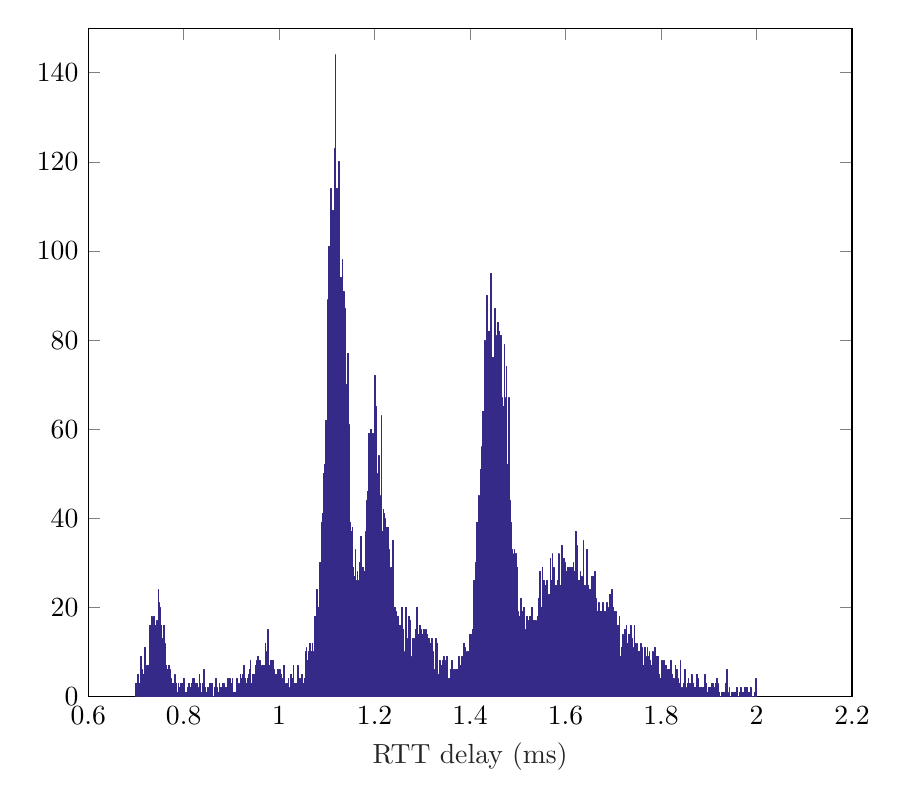
\begin{tikzpicture}

\begin{axis}[%
width=0.8\columnwidth,%7.484in,
height=0.7\columnwidth,%8.26in,
at={(1.255in,1.115in)},
scale only axis,
point meta min=1,
point meta max=2,
colormap={mymap}{[1pt] rgb(0pt)=(0.2081,0.1663,0.5292); rgb(1pt)=(0.211624,0.189781,0.577676); rgb(2pt)=(0.212252,0.213771,0.626971); rgb(3pt)=(0.2081,0.2386,0.677086); rgb(4pt)=(0.195905,0.264457,0.7279); rgb(5pt)=(0.170729,0.291938,0.779248); rgb(6pt)=(0.125271,0.324243,0.830271); rgb(7pt)=(0.0591333,0.359833,0.868333); rgb(8pt)=(0.0116952,0.38751,0.881957); rgb(9pt)=(0.00595714,0.408614,0.882843); rgb(10pt)=(0.0165143,0.4266,0.878633); rgb(11pt)=(0.0328524,0.443043,0.871957); rgb(12pt)=(0.0498143,0.458571,0.864057); rgb(13pt)=(0.0629333,0.47369,0.855438); rgb(14pt)=(0.0722667,0.488667,0.8467); rgb(15pt)=(0.0779429,0.503986,0.838371); rgb(16pt)=(0.0793476,0.520024,0.831181); rgb(17pt)=(0.0749429,0.537543,0.826271); rgb(18pt)=(0.0640571,0.556986,0.823957); rgb(19pt)=(0.0487714,0.577224,0.822829); rgb(20pt)=(0.0343429,0.596581,0.819852); rgb(21pt)=(0.0265,0.6137,0.8135); rgb(22pt)=(0.0238905,0.628662,0.803762); rgb(23pt)=(0.0230905,0.641786,0.791267); rgb(24pt)=(0.0227714,0.653486,0.776757); rgb(25pt)=(0.0266619,0.664195,0.760719); rgb(26pt)=(0.0383714,0.674271,0.743552); rgb(27pt)=(0.0589714,0.683757,0.725386); rgb(28pt)=(0.0843,0.692833,0.706167); rgb(29pt)=(0.113295,0.7015,0.685857); rgb(30pt)=(0.145271,0.709757,0.664629); rgb(31pt)=(0.180133,0.717657,0.642433); rgb(32pt)=(0.217829,0.725043,0.619262); rgb(33pt)=(0.258643,0.731714,0.595429); rgb(34pt)=(0.302171,0.737605,0.571186); rgb(35pt)=(0.348167,0.742433,0.547267); rgb(36pt)=(0.395257,0.7459,0.524443); rgb(37pt)=(0.44201,0.748081,0.503314); rgb(38pt)=(0.487124,0.749062,0.483976); rgb(39pt)=(0.530029,0.749114,0.466114); rgb(40pt)=(0.570857,0.748519,0.44939); rgb(41pt)=(0.609852,0.747314,0.433686); rgb(42pt)=(0.6473,0.7456,0.4188); rgb(43pt)=(0.683419,0.743476,0.404433); rgb(44pt)=(0.71841,0.741133,0.390476); rgb(45pt)=(0.752486,0.7384,0.376814); rgb(46pt)=(0.785843,0.735567,0.363271); rgb(47pt)=(0.818505,0.732733,0.34979); rgb(48pt)=(0.850657,0.7299,0.336029); rgb(49pt)=(0.882433,0.727433,0.3217); rgb(50pt)=(0.913933,0.725786,0.306276); rgb(51pt)=(0.944957,0.726114,0.288643); rgb(52pt)=(0.973895,0.731395,0.266648); rgb(53pt)=(0.993771,0.745457,0.240348); rgb(54pt)=(0.999043,0.765314,0.216414); rgb(55pt)=(0.995533,0.786057,0.196652); rgb(56pt)=(0.988,0.8066,0.179367); rgb(57pt)=(0.978857,0.827143,0.163314); rgb(58pt)=(0.9697,0.848138,0.147452); rgb(59pt)=(0.962586,0.870514,0.1309); rgb(60pt)=(0.958871,0.8949,0.113243); rgb(61pt)=(0.959824,0.921833,0.0948381); rgb(62pt)=(0.9661,0.951443,0.0755333); rgb(63pt)=(0.9763,0.9831,0.0538)},
xmin=0.6,
xmax=2.2,
xlabel style={font=\color{white!15!black}},
xlabel={RTT delay (ms)},
ymin=0,
ymax=150,
axis background/.style={fill=white}
]

\addplot[area legend, table/row sep=crcr, patch, patch type=rectangle, shader=flat corner, forget plot, patch table with point meta={%
1	2	3	4	1\\
6	7	8	9	1\\
11	12	13	14	1\\
16	17	18	19	1\\
21	22	23	24	1\\
26	27	28	29	1\\
31	32	33	34	1\\
36	37	38	39	1\\
41	42	43	44	1\\
46	47	48	49	1\\
51	52	53	54	1\\
56	57	58	59	1\\
61	62	63	64	1\\
66	67	68	69	1\\
71	72	73	74	1\\
76	77	78	79	1\\
81	82	83	84	1\\
86	87	88	89	1\\
91	92	93	94	1\\
96	97	98	99	1\\
101	102	103	104	1\\
106	107	108	109	1\\
111	112	113	114	1\\
116	117	118	119	1\\
121	122	123	124	1\\
126	127	128	129	1\\
131	132	133	134	1\\
136	137	138	139	1\\
141	142	143	144	1\\
146	147	148	149	1\\
151	152	153	154	1\\
156	157	158	159	1\\
161	162	163	164	1\\
166	167	168	169	1\\
171	172	173	174	1\\
176	177	178	179	1\\
181	182	183	184	1\\
186	187	188	189	1\\
191	192	193	194	1\\
196	197	198	199	1\\
201	202	203	204	1\\
206	207	208	209	1\\
211	212	213	214	1\\
216	217	218	219	1\\
221	222	223	224	1\\
226	227	228	229	1\\
231	232	233	234	1\\
236	237	238	239	1\\
241	242	243	244	1\\
246	247	248	249	1\\
251	252	253	254	1\\
256	257	258	259	1\\
261	262	263	264	1\\
266	267	268	269	1\\
271	272	273	274	1\\
276	277	278	279	1\\
281	282	283	284	1\\
286	287	288	289	1\\
291	292	293	294	1\\
296	297	298	299	1\\
301	302	303	304	1\\
306	307	308	309	1\\
311	312	313	314	1\\
316	317	318	319	1\\
321	322	323	324	1\\
326	327	328	329	1\\
331	332	333	334	1\\
336	337	338	339	1\\
341	342	343	344	1\\
346	347	348	349	1\\
351	352	353	354	1\\
356	357	358	359	1\\
361	362	363	364	1\\
366	367	368	369	1\\
371	372	373	374	1\\
376	377	378	379	1\\
381	382	383	384	1\\
386	387	388	389	1\\
391	392	393	394	1\\
396	397	398	399	1\\
401	402	403	404	1\\
406	407	408	409	1\\
411	412	413	414	1\\
416	417	418	419	1\\
421	422	423	424	1\\
426	427	428	429	1\\
431	432	433	434	1\\
436	437	438	439	1\\
441	442	443	444	1\\
446	447	448	449	1\\
451	452	453	454	1\\
456	457	458	459	1\\
461	462	463	464	1\\
466	467	468	469	1\\
471	472	473	474	1\\
476	477	478	479	1\\
481	482	483	484	1\\
486	487	488	489	1\\
491	492	493	494	1\\
496	497	498	499	1\\
501	502	503	504	1\\
506	507	508	509	1\\
511	512	513	514	1\\
516	517	518	519	1\\
521	522	523	524	1\\
526	527	528	529	1\\
531	532	533	534	1\\
536	537	538	539	1\\
541	542	543	544	1\\
546	547	548	549	1\\
551	552	553	554	1\\
556	557	558	559	1\\
561	562	563	564	1\\
566	567	568	569	1\\
571	572	573	574	1\\
576	577	578	579	1\\
581	582	583	584	1\\
586	587	588	589	1\\
591	592	593	594	1\\
596	597	598	599	1\\
601	602	603	604	1\\
606	607	608	609	1\\
611	612	613	614	1\\
616	617	618	619	1\\
621	622	623	624	1\\
626	627	628	629	1\\
631	632	633	634	1\\
636	637	638	639	1\\
641	642	643	644	1\\
646	647	648	649	1\\
651	652	653	654	1\\
656	657	658	659	1\\
661	662	663	664	1\\
666	667	668	669	1\\
671	672	673	674	1\\
676	677	678	679	1\\
681	682	683	684	1\\
686	687	688	689	1\\
691	692	693	694	1\\
696	697	698	699	1\\
701	702	703	704	1\\
706	707	708	709	1\\
711	712	713	714	1\\
716	717	718	719	1\\
721	722	723	724	1\\
726	727	728	729	1\\
731	732	733	734	1\\
736	737	738	739	1\\
741	742	743	744	1\\
746	747	748	749	1\\
751	752	753	754	1\\
756	757	758	759	1\\
761	762	763	764	1\\
766	767	768	769	1\\
771	772	773	774	1\\
776	777	778	779	1\\
781	782	783	784	1\\
786	787	788	789	1\\
791	792	793	794	1\\
796	797	798	799	1\\
801	802	803	804	1\\
806	807	808	809	1\\
811	812	813	814	1\\
816	817	818	819	1\\
821	822	823	824	1\\
826	827	828	829	1\\
831	832	833	834	1\\
836	837	838	839	1\\
841	842	843	844	1\\
846	847	848	849	1\\
851	852	853	854	1\\
856	857	858	859	1\\
861	862	863	864	1\\
866	867	868	869	1\\
871	872	873	874	1\\
876	877	878	879	1\\
881	882	883	884	1\\
886	887	888	889	1\\
891	892	893	894	1\\
896	897	898	899	1\\
901	902	903	904	1\\
906	907	908	909	1\\
911	912	913	914	1\\
916	917	918	919	1\\
921	922	923	924	1\\
926	927	928	929	1\\
931	932	933	934	1\\
936	937	938	939	1\\
941	942	943	944	1\\
946	947	948	949	1\\
951	952	953	954	1\\
956	957	958	959	1\\
961	962	963	964	1\\
966	967	968	969	1\\
971	972	973	974	1\\
976	977	978	979	1\\
981	982	983	984	1\\
986	987	988	989	1\\
991	992	993	994	1\\
996	997	998	999	1\\
1001	1002	1003	1004	1\\
1006	1007	1008	1009	1\\
1011	1012	1013	1014	1\\
1016	1017	1018	1019	1\\
1021	1022	1023	1024	1\\
1026	1027	1028	1029	1\\
1031	1032	1033	1034	1\\
1036	1037	1038	1039	1\\
1041	1042	1043	1044	1\\
1046	1047	1048	1049	1\\
1051	1052	1053	1054	1\\
1056	1057	1058	1059	1\\
1061	1062	1063	1064	1\\
1066	1067	1068	1069	1\\
1071	1072	1073	1074	1\\
1076	1077	1078	1079	1\\
1081	1082	1083	1084	1\\
1086	1087	1088	1089	1\\
1091	1092	1093	1094	1\\
1096	1097	1098	1099	1\\
1101	1102	1103	1104	1\\
1106	1107	1108	1109	1\\
1111	1112	1113	1114	1\\
1116	1117	1118	1119	1\\
1121	1122	1123	1124	1\\
1126	1127	1128	1129	1\\
1131	1132	1133	1134	1\\
1136	1137	1138	1139	1\\
1141	1142	1143	1144	1\\
1146	1147	1148	1149	1\\
1151	1152	1153	1154	1\\
1156	1157	1158	1159	1\\
1161	1162	1163	1164	1\\
1166	1167	1168	1169	1\\
1171	1172	1173	1174	1\\
1176	1177	1178	1179	1\\
1181	1182	1183	1184	1\\
1186	1187	1188	1189	1\\
1191	1192	1193	1194	1\\
1196	1197	1198	1199	1\\
1201	1202	1203	1204	1\\
1206	1207	1208	1209	1\\
1211	1212	1213	1214	1\\
1216	1217	1218	1219	1\\
1221	1222	1223	1224	1\\
1226	1227	1228	1229	1\\
1231	1232	1233	1234	1\\
1236	1237	1238	1239	1\\
1241	1242	1243	1244	1\\
1246	1247	1248	1249	1\\
1251	1252	1253	1254	1\\
1256	1257	1258	1259	1\\
1261	1262	1263	1264	1\\
1266	1267	1268	1269	1\\
1271	1272	1273	1274	1\\
1276	1277	1278	1279	1\\
1281	1282	1283	1284	1\\
1286	1287	1288	1289	1\\
1291	1292	1293	1294	1\\
1296	1297	1298	1299	1\\
1301	1302	1303	1304	1\\
1306	1307	1308	1309	1\\
1311	1312	1313	1314	1\\
1316	1317	1318	1319	1\\
1321	1322	1323	1324	1\\
1326	1327	1328	1329	1\\
1331	1332	1333	1334	1\\
1336	1337	1338	1339	1\\
1341	1342	1343	1344	1\\
1346	1347	1348	1349	1\\
1351	1352	1353	1354	1\\
1356	1357	1358	1359	1\\
1361	1362	1363	1364	1\\
1366	1367	1368	1369	1\\
1371	1372	1373	1374	1\\
1376	1377	1378	1379	1\\
1381	1382	1383	1384	1\\
1386	1387	1388	1389	1\\
1391	1392	1393	1394	1\\
1396	1397	1398	1399	1\\
1401	1402	1403	1404	1\\
1406	1407	1408	1409	1\\
1411	1412	1413	1414	1\\
1416	1417	1418	1419	1\\
1421	1422	1423	1424	1\\
1426	1427	1428	1429	1\\
1431	1432	1433	1434	1\\
1436	1437	1438	1439	1\\
1441	1442	1443	1444	1\\
1446	1447	1448	1449	1\\
1451	1452	1453	1454	1\\
1456	1457	1458	1459	1\\
1461	1462	1463	1464	1\\
1466	1467	1468	1469	1\\
1471	1472	1473	1474	1\\
1476	1477	1478	1479	1\\
1481	1482	1483	1484	1\\
1486	1487	1488	1489	1\\
1491	1492	1493	1494	1\\
1496	1497	1498	1499	1\\
1501	1502	1503	1504	1\\
1506	1507	1508	1509	1\\
1511	1512	1513	1514	1\\
1516	1517	1518	1519	1\\
1521	1522	1523	1524	1\\
1526	1527	1528	1529	1\\
1531	1532	1533	1534	1\\
1536	1537	1538	1539	1\\
1541	1542	1543	1544	1\\
1546	1547	1548	1549	1\\
1551	1552	1553	1554	1\\
1556	1557	1558	1559	1\\
1561	1562	1563	1564	1\\
1566	1567	1568	1569	1\\
1571	1572	1573	1574	1\\
1576	1577	1578	1579	1\\
1581	1582	1583	1584	1\\
1586	1587	1588	1589	1\\
1591	1592	1593	1594	1\\
1596	1597	1598	1599	1\\
1601	1602	1603	1604	1\\
1606	1607	1608	1609	1\\
1611	1612	1613	1614	1\\
1616	1617	1618	1619	1\\
1621	1622	1623	1624	1\\
1626	1627	1628	1629	1\\
1631	1632	1633	1634	1\\
1636	1637	1638	1639	1\\
1641	1642	1643	1644	1\\
1646	1647	1648	1649	1\\
1651	1652	1653	1654	1\\
1656	1657	1658	1659	1\\
1661	1662	1663	1664	1\\
1666	1667	1668	1669	1\\
1671	1672	1673	1674	1\\
1676	1677	1678	1679	1\\
1681	1682	1683	1684	1\\
1686	1687	1688	1689	1\\
1691	1692	1693	1694	1\\
1696	1697	1698	1699	1\\
1701	1702	1703	1704	1\\
1706	1707	1708	1709	1\\
1711	1712	1713	1714	1\\
1716	1717	1718	1719	1\\
1721	1722	1723	1724	1\\
1726	1727	1728	1729	1\\
1731	1732	1733	1734	1\\
1736	1737	1738	1739	1\\
1741	1742	1743	1744	1\\
1746	1747	1748	1749	1\\
1751	1752	1753	1754	1\\
1756	1757	1758	1759	1\\
1761	1762	1763	1764	1\\
1766	1767	1768	1769	1\\
1771	1772	1773	1774	1\\
1776	1777	1778	1779	1\\
1781	1782	1783	1784	1\\
1786	1787	1788	1789	1\\
1791	1792	1793	1794	1\\
1796	1797	1798	1799	1\\
1801	1802	1803	1804	1\\
1806	1807	1808	1809	1\\
1811	1812	1813	1814	1\\
1816	1817	1818	1819	1\\
1821	1822	1823	1824	1\\
1826	1827	1828	1829	1\\
1831	1832	1833	1834	1\\
1836	1837	1838	1839	1\\
1841	1842	1843	1844	1\\
1846	1847	1848	1849	1\\
1851	1852	1853	1854	1\\
1856	1857	1858	1859	1\\
1861	1862	1863	1864	1\\
1866	1867	1868	1869	1\\
1871	1872	1873	1874	1\\
1876	1877	1878	1879	1\\
1881	1882	1883	1884	1\\
1886	1887	1888	1889	1\\
1891	1892	1893	1894	1\\
1896	1897	1898	1899	1\\
1901	1902	1903	1904	1\\
1906	1907	1908	1909	1\\
1911	1912	1913	1914	1\\
1916	1917	1918	1919	1\\
1921	1922	1923	1924	1\\
1926	1927	1928	1929	1\\
1931	1932	1933	1934	1\\
1936	1937	1938	1939	1\\
1941	1942	1943	1944	1\\
1946	1947	1948	1949	1\\
1951	1952	1953	1954	1\\
1956	1957	1958	1959	1\\
1961	1962	1963	1964	1\\
1966	1967	1968	1969	1\\
1971	1972	1973	1974	1\\
1976	1977	1978	1979	1\\
1981	1982	1983	1984	1\\
1986	1987	1988	1989	1\\
1991	1992	1993	1994	1\\
1996	1997	1998	1999	1\\
2001	2002	2003	2004	1\\
2006	2007	2008	2009	1\\
2011	2012	2013	2014	1\\
2016	2017	2018	2019	1\\
2021	2022	2023	2024	1\\
2026	2027	2028	2029	1\\
2031	2032	2033	2034	1\\
2036	2037	2038	2039	1\\
2041	2042	2043	2044	1\\
2046	2047	2048	2049	1\\
2051	2052	2053	2054	1\\
2056	2057	2058	2059	1\\
2061	2062	2063	2064	1\\
2066	2067	2068	2069	1\\
2071	2072	2073	2074	1\\
2076	2077	2078	2079	1\\
2081	2082	2083	2084	1\\
2086	2087	2088	2089	1\\
2091	2092	2093	2094	1\\
2096	2097	2098	2099	1\\
2101	2102	2103	2104	1\\
2106	2107	2108	2109	1\\
2111	2112	2113	2114	1\\
2116	2117	2118	2119	1\\
2121	2122	2123	2124	1\\
2126	2127	2128	2129	1\\
2131	2132	2133	2134	1\\
2136	2137	2138	2139	1\\
2141	2142	2143	2144	1\\
2146	2147	2148	2149	1\\
2151	2152	2153	2154	1\\
2156	2157	2158	2159	1\\
2161	2162	2163	2164	1\\
2166	2167	2168	2169	1\\
2171	2172	2173	2174	1\\
2176	2177	2178	2179	1\\
2181	2182	2183	2184	1\\
2186	2187	2188	2189	1\\
2191	2192	2193	2194	1\\
2196	2197	2198	2199	1\\
2201	2202	2203	2204	1\\
2206	2207	2208	2209	1\\
2211	2212	2213	2214	1\\
2216	2217	2218	2219	1\\
2221	2222	2223	2224	1\\
2226	2227	2228	2229	1\\
2231	2232	2233	2234	1\\
2236	2237	2238	2239	1\\
2241	2242	2243	2244	1\\
2246	2247	2248	2249	1\\
2251	2252	2253	2254	1\\
2256	2257	2258	2259	1\\
2261	2262	2263	2264	1\\
2266	2267	2268	2269	1\\
2271	2272	2273	2274	1\\
2276	2277	2278	2279	1\\
2281	2282	2283	2284	1\\
2286	2287	2288	2289	1\\
2291	2292	2293	2294	1\\
2296	2297	2298	2299	1\\
2301	2302	2303	2304	1\\
2306	2307	2308	2309	1\\
2311	2312	2313	2314	1\\
2316	2317	2318	2319	1\\
2321	2322	2323	2324	1\\
2326	2327	2328	2329	1\\
2331	2332	2333	2334	1\\
2336	2337	2338	2339	1\\
2341	2342	2343	2344	1\\
2346	2347	2348	2349	1\\
2351	2352	2353	2354	1\\
2356	2357	2358	2359	1\\
2361	2362	2363	2364	1\\
2366	2367	2368	2369	1\\
2371	2372	2373	2374	1\\
2376	2377	2378	2379	1\\
2381	2382	2383	2384	1\\
2386	2387	2388	2389	1\\
2391	2392	2393	2394	1\\
2396	2397	2398	2399	1\\
2401	2402	2403	2404	1\\
2406	2407	2408	2409	1\\
2411	2412	2413	2414	1\\
2416	2417	2418	2419	1\\
2421	2422	2423	2424	1\\
2426	2427	2428	2429	1\\
2431	2432	2433	2434	1\\
2436	2437	2438	2439	1\\
2441	2442	2443	2444	1\\
2446	2447	2448	2449	1\\
2451	2452	2453	2454	1\\
2456	2457	2458	2459	1\\
2461	2462	2463	2464	1\\
2466	2467	2468	2469	1\\
2471	2472	2473	2474	1\\
2476	2477	2478	2479	1\\
2481	2482	2483	2484	1\\
2486	2487	2488	2489	1\\
2491	2492	2493	2494	1\\
2496	2497	2498	2499	1\\
2501	2502	2503	2504	1\\
2506	2507	2508	2509	1\\
2511	2512	2513	2514	1\\
2516	2517	2518	2519	1\\
2521	2522	2523	2524	1\\
2526	2527	2528	2529	1\\
2531	2532	2533	2534	1\\
2536	2537	2538	2539	1\\
2541	2542	2543	2544	1\\
2546	2547	2548	2549	1\\
2551	2552	2553	2554	1\\
2556	2557	2558	2559	1\\
2561	2562	2563	2564	1\\
2566	2567	2568	2569	1\\
2571	2572	2573	2574	1\\
2576	2577	2578	2579	1\\
2581	2582	2583	2584	1\\
2586	2587	2588	2589	1\\
2591	2592	2593	2594	1\\
2596	2597	2598	2599	1\\
2601	2602	2603	2604	1\\
2606	2607	2608	2609	1\\
2611	2612	2613	2614	1\\
2616	2617	2618	2619	1\\
2621	2622	2623	2624	1\\
2626	2627	2628	2629	1\\
2631	2632	2633	2634	1\\
2636	2637	2638	2639	1\\
2641	2642	2643	2644	1\\
2646	2647	2648	2649	1\\
2651	2652	2653	2654	1\\
2656	2657	2658	2659	1\\
2661	2662	2663	2664	1\\
2666	2667	2668	2669	1\\
2671	2672	2673	2674	1\\
2676	2677	2678	2679	1\\
2681	2682	2683	2684	1\\
2686	2687	2688	2689	1\\
2691	2692	2693	2694	1\\
2696	2697	2698	2699	1\\
2701	2702	2703	2704	1\\
2706	2707	2708	2709	1\\
2711	2712	2713	2714	1\\
2716	2717	2718	2719	1\\
2721	2722	2723	2724	1\\
2726	2727	2728	2729	1\\
2731	2732	2733	2734	1\\
2736	2737	2738	2739	1\\
2741	2742	2743	2744	1\\
2746	2747	2748	2749	1\\
2751	2752	2753	2754	1\\
2756	2757	2758	2759	1\\
2761	2762	2763	2764	1\\
2766	2767	2768	2769	1\\
2771	2772	2773	2774	1\\
2776	2777	2778	2779	1\\
2781	2782	2783	2784	1\\
2786	2787	2788	2789	1\\
2791	2792	2793	2794	1\\
2796	2797	2798	2799	1\\
2801	2802	2803	2804	1\\
2806	2807	2808	2809	1\\
2811	2812	2813	2814	1\\
2816	2817	2818	2819	1\\
2821	2822	2823	2824	1\\
2826	2827	2828	2829	1\\
2831	2832	2833	2834	1\\
2836	2837	2838	2839	1\\
2841	2842	2843	2844	1\\
2846	2847	2848	2849	1\\
2851	2852	2853	2854	1\\
2856	2857	2858	2859	1\\
2861	2862	2863	2864	1\\
2866	2867	2868	2869	1\\
2871	2872	2873	2874	1\\
2876	2877	2878	2879	1\\
2881	2882	2883	2884	1\\
2886	2887	2888	2889	1\\
2891	2892	2893	2894	1\\
2896	2897	2898	2899	1\\
2901	2902	2903	2904	1\\
2906	2907	2908	2909	1\\
2911	2912	2913	2914	1\\
2916	2917	2918	2919	1\\
2921	2922	2923	2924	1\\
2926	2927	2928	2929	1\\
2931	2932	2933	2934	1\\
2936	2937	2938	2939	1\\
2941	2942	2943	2944	1\\
2946	2947	2948	2949	1\\
2951	2952	2953	2954	1\\
2956	2957	2958	2959	1\\
2961	2962	2963	2964	1\\
2966	2967	2968	2969	1\\
2971	2972	2973	2974	1\\
2976	2977	2978	2979	1\\
2981	2982	2983	2984	1\\
2986	2987	2988	2989	1\\
2991	2992	2993	2994	1\\
2996	2997	2998	2999	1\\
3001	3002	3003	3004	1\\
3006	3007	3008	3009	1\\
3011	3012	3013	3014	1\\
3016	3017	3018	3019	1\\
3021	3022	3023	3024	1\\
3026	3027	3028	3029	1\\
3031	3032	3033	3034	1\\
3036	3037	3038	3039	1\\
3041	3042	3043	3044	1\\
3046	3047	3048	3049	1\\
3051	3052	3053	3054	1\\
3056	3057	3058	3059	1\\
3061	3062	3063	3064	1\\
3066	3067	3068	3069	1\\
3071	3072	3073	3074	1\\
3076	3077	3078	3079	1\\
3081	3082	3083	3084	1\\
3086	3087	3088	3089	1\\
3091	3092	3093	3094	1\\
3096	3097	3098	3099	1\\
3101	3102	3103	3104	1\\
3106	3107	3108	3109	1\\
3111	3112	3113	3114	1\\
3116	3117	3118	3119	1\\
3121	3122	3123	3124	1\\
3126	3127	3128	3129	1\\
3131	3132	3133	3134	1\\
3136	3137	3138	3139	1\\
3141	3142	3143	3144	1\\
3146	3147	3148	3149	1\\
3151	3152	3153	3154	1\\
3156	3157	3158	3159	1\\
3161	3162	3163	3164	1\\
3166	3167	3168	3169	1\\
3171	3172	3173	3174	1\\
3176	3177	3178	3179	1\\
3181	3182	3183	3184	1\\
3186	3187	3188	3189	1\\
3191	3192	3193	3194	1\\
3196	3197	3198	3199	1\\
3201	3202	3203	3204	1\\
3206	3207	3208	3209	1\\
3211	3212	3213	3214	1\\
3216	3217	3218	3219	1\\
3221	3222	3223	3224	1\\
3226	3227	3228	3229	1\\
3231	3232	3233	3234	1\\
3236	3237	3238	3239	1\\
3241	3242	3243	3244	1\\
3246	3247	3248	3249	1\\
3251	3252	3253	3254	1\\
3256	3257	3258	3259	1\\
3261	3262	3263	3264	1\\
3266	3267	3268	3269	1\\
3271	3272	3273	3274	1\\
3276	3277	3278	3279	1\\
3281	3282	3283	3284	1\\
3286	3287	3288	3289	1\\
3291	3292	3293	3294	1\\
3296	3297	3298	3299	1\\
3301	3302	3303	3304	1\\
3306	3307	3308	3309	1\\
3311	3312	3313	3314	1\\
3316	3317	3318	3319	1\\
3321	3322	3323	3324	1\\
3326	3327	3328	3329	1\\
3331	3332	3333	3334	1\\
3336	3337	3338	3339	1\\
3341	3342	3343	3344	1\\
3346	3347	3348	3349	1\\
3351	3352	3353	3354	1\\
3356	3357	3358	3359	1\\
3361	3362	3363	3364	1\\
3366	3367	3368	3369	1\\
3371	3372	3373	3374	1\\
3376	3377	3378	3379	1\\
3381	3382	3383	3384	1\\
3386	3387	3388	3389	1\\
3391	3392	3393	3394	1\\
3396	3397	3398	3399	1\\
3401	3402	3403	3404	1\\
3406	3407	3408	3409	1\\
3411	3412	3413	3414	1\\
3416	3417	3418	3419	1\\
3421	3422	3423	3424	1\\
3426	3427	3428	3429	1\\
3431	3432	3433	3434	1\\
3436	3437	3438	3439	1\\
3441	3442	3443	3444	1\\
3446	3447	3448	3449	1\\
3451	3452	3453	3454	1\\
3456	3457	3458	3459	1\\
3461	3462	3463	3464	1\\
3466	3467	3468	3469	1\\
3471	3472	3473	3474	1\\
3476	3477	3478	3479	1\\
3481	3482	3483	3484	1\\
3486	3487	3488	3489	1\\
3491	3492	3493	3494	1\\
3496	3497	3498	3499	1\\
3501	3502	3503	3504	1\\
3506	3507	3508	3509	1\\
3511	3512	3513	3514	1\\
3516	3517	3518	3519	1\\
3521	3522	3523	3524	1\\
3526	3527	3528	3529	1\\
3531	3532	3533	3534	1\\
3536	3537	3538	3539	1\\
3541	3542	3543	3544	1\\
3546	3547	3548	3549	1\\
3551	3552	3553	3554	1\\
3556	3557	3558	3559	1\\
3561	3562	3563	3564	1\\
3566	3567	3568	3569	1\\
3571	3572	3573	3574	1\\
3576	3577	3578	3579	1\\
3581	3582	3583	3584	1\\
3586	3587	3588	3589	1\\
3591	3592	3593	3594	1\\
3596	3597	3598	3599	1\\
3601	3602	3603	3604	1\\
3606	3607	3608	3609	1\\
3611	3612	3613	3614	1\\
3616	3617	3618	3619	1\\
3621	3622	3623	3624	1\\
3626	3627	3628	3629	1\\
3631	3632	3633	3634	1\\
3636	3637	3638	3639	1\\
3641	3642	3643	3644	1\\
3646	3647	3648	3649	1\\
3651	3652	3653	3654	1\\
3656	3657	3658	3659	1\\
3661	3662	3663	3664	1\\
3666	3667	3668	3669	1\\
3671	3672	3673	3674	1\\
3676	3677	3678	3679	1\\
3681	3682	3683	3684	1\\
3686	3687	3688	3689	1\\
3691	3692	3693	3694	1\\
3696	3697	3698	3699	1\\
3701	3702	3703	3704	1\\
3706	3707	3708	3709	1\\
3711	3712	3713	3714	1\\
3716	3717	3718	3719	1\\
3721	3722	3723	3724	1\\
3726	3727	3728	3729	1\\
3731	3732	3733	3734	1\\
3736	3737	3738	3739	1\\
3741	3742	3743	3744	1\\
3746	3747	3748	3749	1\\
3751	3752	3753	3754	1\\
3756	3757	3758	3759	1\\
3761	3762	3763	3764	1\\
3766	3767	3768	3769	1\\
3771	3772	3773	3774	1\\
3776	3777	3778	3779	1\\
3781	3782	3783	3784	1\\
3786	3787	3788	3789	1\\
3791	3792	3793	3794	1\\
3796	3797	3798	3799	1\\
3801	3802	3803	3804	1\\
3806	3807	3808	3809	1\\
3811	3812	3813	3814	1\\
3816	3817	3818	3819	1\\
3821	3822	3823	3824	1\\
3826	3827	3828	3829	1\\
3831	3832	3833	3834	1\\
3836	3837	3838	3839	1\\
3841	3842	3843	3844	1\\
3846	3847	3848	3849	1\\
3851	3852	3853	3854	1\\
3856	3857	3858	3859	1\\
3861	3862	3863	3864	1\\
3866	3867	3868	3869	1\\
3871	3872	3873	3874	1\\
3876	3877	3878	3879	1\\
3881	3882	3883	3884	1\\
3886	3887	3888	3889	1\\
3891	3892	3893	3894	1\\
3896	3897	3898	3899	1\\
3901	3902	3903	3904	1\\
3906	3907	3908	3909	1\\
3911	3912	3913	3914	1\\
3916	3917	3918	3919	1\\
3921	3922	3923	3924	1\\
3926	3927	3928	3929	1\\
3931	3932	3933	3934	1\\
3936	3937	3938	3939	1\\
3941	3942	3943	3944	1\\
3946	3947	3948	3949	1\\
3951	3952	3953	3954	1\\
3956	3957	3958	3959	1\\
3961	3962	3963	3964	1\\
3966	3967	3968	3969	1\\
3971	3972	3973	3974	1\\
3976	3977	3978	3979	1\\
3981	3982	3983	3984	1\\
3986	3987	3988	3989	1\\
3991	3992	3993	3994	1\\
3996	3997	3998	3999	1\\
4001	4002	4003	4004	1\\
4006	4007	4008	4009	1\\
4011	4012	4013	4014	1\\
4016	4017	4018	4019	1\\
4021	4022	4023	4024	1\\
4026	4027	4028	4029	1\\
4031	4032	4033	4034	1\\
4036	4037	4038	4039	1\\
4041	4042	4043	4044	1\\
4046	4047	4048	4049	1\\
4051	4052	4053	4054	1\\
4056	4057	4058	4059	1\\
4061	4062	4063	4064	1\\
4066	4067	4068	4069	1\\
4071	4072	4073	4074	1\\
4076	4077	4078	4079	1\\
4081	4082	4083	4084	1\\
4086	4087	4088	4089	1\\
4091	4092	4093	4094	1\\
4096	4097	4098	4099	1\\
4101	4102	4103	4104	1\\
4106	4107	4108	4109	1\\
4111	4112	4113	4114	1\\
4116	4117	4118	4119	1\\
4121	4122	4123	4124	1\\
4126	4127	4128	4129	1\\
4131	4132	4133	4134	1\\
4136	4137	4138	4139	1\\
4141	4142	4143	4144	1\\
4146	4147	4148	4149	1\\
4151	4152	4153	4154	1\\
4156	4157	4158	4159	1\\
4161	4162	4163	4164	1\\
4166	4167	4168	4169	1\\
4171	4172	4173	4174	1\\
4176	4177	4178	4179	1\\
4181	4182	4183	4184	1\\
4186	4187	4188	4189	1\\
4191	4192	4193	4194	1\\
4196	4197	4198	4199	1\\
4201	4202	4203	4204	1\\
4206	4207	4208	4209	1\\
4211	4212	4213	4214	1\\
4216	4217	4218	4219	1\\
4221	4222	4223	4224	1\\
4226	4227	4228	4229	1\\
4231	4232	4233	4234	1\\
4236	4237	4238	4239	1\\
4241	4242	4243	4244	1\\
4246	4247	4248	4249	1\\
4251	4252	4253	4254	1\\
4256	4257	4258	4259	1\\
4261	4262	4263	4264	1\\
4266	4267	4268	4269	1\\
4271	4272	4273	4274	1\\
4276	4277	4278	4279	1\\
4281	4282	4283	4284	1\\
4286	4287	4288	4289	1\\
4291	4292	4293	4294	1\\
4296	4297	4298	4299	1\\
4301	4302	4303	4304	1\\
4306	4307	4308	4309	1\\
4311	4312	4313	4314	1\\
4316	4317	4318	4319	1\\
4321	4322	4323	4324	1\\
4326	4327	4328	4329	1\\
4331	4332	4333	4334	1\\
4336	4337	4338	4339	1\\
4341	4342	4343	4344	1\\
4346	4347	4348	4349	1\\
4351	4352	4353	4354	1\\
4356	4357	4358	4359	1\\
4361	4362	4363	4364	1\\
4366	4367	4368	4369	1\\
4371	4372	4373	4374	1\\
4376	4377	4378	4379	1\\
4381	4382	4383	4384	1\\
4386	4387	4388	4389	1\\
4391	4392	4393	4394	1\\
4396	4397	4398	4399	1\\
4401	4402	4403	4404	1\\
4406	4407	4408	4409	1\\
4411	4412	4413	4414	1\\
4416	4417	4418	4419	1\\
4421	4422	4423	4424	1\\
4426	4427	4428	4429	1\\
4431	4432	4433	4434	1\\
4436	4437	4438	4439	1\\
4441	4442	4443	4444	1\\
4446	4447	4448	4449	1\\
4451	4452	4453	4454	1\\
4456	4457	4458	4459	1\\
4461	4462	4463	4464	1\\
4466	4467	4468	4469	1\\
4471	4472	4473	4474	1\\
4476	4477	4478	4479	1\\
4481	4482	4483	4484	1\\
4486	4487	4488	4489	1\\
4491	4492	4493	4494	1\\
4496	4497	4498	4499	1\\
4501	4502	4503	4504	1\\
4506	4507	4508	4509	1\\
4511	4512	4513	4514	1\\
4516	4517	4518	4519	1\\
4521	4522	4523	4524	1\\
4526	4527	4528	4529	1\\
4531	4532	4533	4534	1\\
4536	4537	4538	4539	1\\
4541	4542	4543	4544	1\\
4546	4547	4548	4549	1\\
4551	4552	4553	4554	1\\
4556	4557	4558	4559	1\\
4561	4562	4563	4564	1\\
4566	4567	4568	4569	1\\
4571	4572	4573	4574	1\\
4576	4577	4578	4579	1\\
4581	4582	4583	4584	1\\
4586	4587	4588	4589	1\\
4591	4592	4593	4594	1\\
4596	4597	4598	4599	1\\
4601	4602	4603	4604	1\\
4606	4607	4608	4609	1\\
4611	4612	4613	4614	1\\
4616	4617	4618	4619	1\\
4621	4622	4623	4624	1\\
4626	4627	4628	4629	1\\
4631	4632	4633	4634	1\\
4636	4637	4638	4639	1\\
4641	4642	4643	4644	1\\
4646	4647	4648	4649	1\\
4651	4652	4653	4654	1\\
4656	4657	4658	4659	1\\
4661	4662	4663	4664	1\\
4666	4667	4668	4669	1\\
4671	4672	4673	4674	1\\
4676	4677	4678	4679	1\\
4681	4682	4683	4684	1\\
4686	4687	4688	4689	1\\
4691	4692	4693	4694	1\\
4696	4697	4698	4699	1\\
4701	4702	4703	4704	1\\
4706	4707	4708	4709	1\\
4711	4712	4713	4714	1\\
4716	4717	4718	4719	1\\
4721	4722	4723	4724	1\\
4726	4727	4728	4729	1\\
4731	4732	4733	4734	1\\
4736	4737	4738	4739	1\\
4741	4742	4743	4744	1\\
4746	4747	4748	4749	1\\
4751	4752	4753	4754	1\\
4756	4757	4758	4759	1\\
4761	4762	4763	4764	1\\
4766	4767	4768	4769	1\\
4771	4772	4773	4774	1\\
4776	4777	4778	4779	1\\
4781	4782	4783	4784	1\\
4786	4787	4788	4789	1\\
4791	4792	4793	4794	1\\
4796	4797	4798	4799	1\\
4801	4802	4803	4804	1\\
4806	4807	4808	4809	1\\
4811	4812	4813	4814	1\\
4816	4817	4818	4819	1\\
4821	4822	4823	4824	1\\
4826	4827	4828	4829	1\\
4831	4832	4833	4834	1\\
4836	4837	4838	4839	1\\
4841	4842	4843	4844	1\\
4846	4847	4848	4849	1\\
4851	4852	4853	4854	1\\
4856	4857	4858	4859	1\\
4861	4862	4863	4864	1\\
4866	4867	4868	4869	1\\
4871	4872	4873	4874	1\\
4876	4877	4878	4879	1\\
4881	4882	4883	4884	1\\
4886	4887	4888	4889	1\\
4891	4892	4893	4894	1\\
4896	4897	4898	4899	1\\
4901	4902	4903	4904	1\\
4906	4907	4908	4909	1\\
4911	4912	4913	4914	1\\
4916	4917	4918	4919	1\\
4921	4922	4923	4924	1\\
4926	4927	4928	4929	1\\
4931	4932	4933	4934	1\\
4936	4937	4938	4939	1\\
4941	4942	4943	4944	1\\
4946	4947	4948	4949	1\\
4951	4952	4953	4954	1\\
4956	4957	4958	4959	1\\
4961	4962	4963	4964	1\\
4966	4967	4968	4969	1\\
4971	4972	4973	4974	1\\
4976	4977	4978	4979	1\\
4981	4982	4983	4984	1\\
4986	4987	4988	4989	1\\
4991	4992	4993	4994	1\\
4996	4997	4998	4999	1\\
}]
table[row sep=crcr] {%
x	y\\
0.698566436767578	0\\
0.698566436767578	0\\
0.698566436767578	1\\
0.699867963790894	1\\
0.699867963790894	0\\
0.699867963790894	0\\
0.699867963790894	0\\
0.699867963790894	3\\
0.701169490814209	3\\
0.701169490814209	0\\
0.701169490814209	0\\
0.701169490814209	0\\
0.701169490814209	2\\
0.702471017837524	2\\
0.702471017837524	0\\
0.702471017837524	0\\
0.702471017837524	0\\
0.702471017837524	2\\
0.70377254486084	2\\
0.70377254486084	0\\
0.70377254486084	0\\
0.70377254486084	0\\
0.70377254486084	5\\
0.705074071884155	5\\
0.705074071884155	0\\
0.705074071884155	0\\
0.705074071884155	0\\
0.705074071884155	0\\
0.706375598907471	0\\
0.706375598907471	0\\
0.706375598907471	0\\
0.706375598907471	0\\
0.706375598907471	1\\
0.707677125930786	1\\
0.707677125930786	0\\
0.707677125930786	0\\
0.707677125930786	0\\
0.707677125930786	3\\
0.708978652954102	3\\
0.708978652954102	0\\
0.708978652954102	0\\
0.708978652954102	0\\
0.708978652954102	5\\
0.710280179977417	5\\
0.710280179977417	0\\
0.710280179977417	0\\
0.710280179977417	0\\
0.710280179977417	9\\
0.711581707000732	9\\
0.711581707000732	0\\
0.711581707000732	0\\
0.711581707000732	0\\
0.711581707000732	6\\
0.712883234024048	6\\
0.712883234024048	0\\
0.712883234024048	0\\
0.712883234024048	0\\
0.712883234024048	3\\
0.714184761047363	3\\
0.714184761047363	0\\
0.714184761047363	0\\
0.714184761047363	0\\
0.714184761047363	5\\
0.715486288070679	5\\
0.715486288070679	0\\
0.715486288070679	0\\
0.715486288070679	0\\
0.715486288070679	3\\
0.716787815093994	3\\
0.716787815093994	0\\
0.716787815093994	0\\
0.716787815093994	0\\
0.716787815093994	5\\
0.71808934211731	5\\
0.71808934211731	0\\
0.71808934211731	0\\
0.71808934211731	0\\
0.71808934211731	11\\
0.719390869140625	11\\
0.719390869140625	0\\
0.719390869140625	0\\
0.719390869140625	0\\
0.719390869140625	5\\
0.72069239616394	5\\
0.72069239616394	0\\
0.72069239616394	0\\
0.72069239616394	0\\
0.72069239616394	5\\
0.721993923187256	5\\
0.721993923187256	0\\
0.721993923187256	0\\
0.721993923187256	0\\
0.721993923187256	6\\
0.723295450210571	6\\
0.723295450210571	0\\
0.723295450210571	0\\
0.723295450210571	0\\
0.723295450210571	7\\
0.724596977233887	7\\
0.724596977233887	0\\
0.724596977233887	0\\
0.724596977233887	0\\
0.724596977233887	4\\
0.725898504257202	4\\
0.725898504257202	0\\
0.725898504257202	0\\
0.725898504257202	0\\
0.725898504257202	7\\
0.727200031280518	7\\
0.727200031280518	0\\
0.727200031280518	0\\
0.727200031280518	0\\
0.727200031280518	4\\
0.728501558303833	4\\
0.728501558303833	0\\
0.728501558303833	0\\
0.728501558303833	0\\
0.728501558303833	16\\
0.729803085327148	16\\
0.729803085327148	0\\
0.729803085327148	0\\
0.729803085327148	0\\
0.729803085327148	10\\
0.731104612350464	10\\
0.731104612350464	0\\
0.731104612350464	0\\
0.731104612350464	0\\
0.731104612350464	10\\
0.732406139373779	10\\
0.732406139373779	0\\
0.732406139373779	0\\
0.732406139373779	0\\
0.732406139373779	18\\
0.733707666397095	18\\
0.733707666397095	0\\
0.733707666397095	0\\
0.733707666397095	0\\
0.733707666397095	4\\
0.73500919342041	4\\
0.73500919342041	0\\
0.73500919342041	0\\
0.73500919342041	0\\
0.73500919342041	13\\
0.736310720443726	13\\
0.736310720443726	0\\
0.736310720443726	0\\
0.736310720443726	0\\
0.736310720443726	17\\
0.737612247467041	17\\
0.737612247467041	0\\
0.737612247467041	0\\
0.737612247467041	0\\
0.737612247467041	18\\
0.738913774490356	18\\
0.738913774490356	0\\
0.738913774490356	0\\
0.738913774490356	0\\
0.738913774490356	14\\
0.740215301513672	14\\
0.740215301513672	0\\
0.740215301513672	0\\
0.740215301513672	0\\
0.740215301513672	16\\
0.741516828536987	16\\
0.741516828536987	0\\
0.741516828536987	0\\
0.741516828536987	0\\
0.741516828536987	13\\
0.742818355560303	13\\
0.742818355560303	0\\
0.742818355560303	0\\
0.742818355560303	0\\
0.742818355560303	16\\
0.744119882583618	16\\
0.744119882583618	0\\
0.744119882583618	0\\
0.744119882583618	0\\
0.744119882583618	17\\
0.745421409606934	17\\
0.745421409606934	0\\
0.745421409606934	0\\
0.745421409606934	0\\
0.745421409606934	14\\
0.746722936630249	14\\
0.746722936630249	0\\
0.746722936630249	0\\
0.746722936630249	0\\
0.746722936630249	24\\
0.748024463653564	24\\
0.748024463653564	0\\
0.748024463653564	0\\
0.748024463653564	0\\
0.748024463653564	21\\
0.74932599067688	21\\
0.74932599067688	0\\
0.74932599067688	0\\
0.74932599067688	0\\
0.74932599067688	20\\
0.750627517700195	20\\
0.750627517700195	0\\
0.750627517700195	0\\
0.750627517700195	0\\
0.750627517700195	13\\
0.751929044723511	13\\
0.751929044723511	0\\
0.751929044723511	0\\
0.751929044723511	0\\
0.751929044723511	16\\
0.753230571746826	16\\
0.753230571746826	0\\
0.753230571746826	0\\
0.753230571746826	0\\
0.753230571746826	12\\
0.754532098770142	12\\
0.754532098770142	0\\
0.754532098770142	0\\
0.754532098770142	0\\
0.754532098770142	13\\
0.755833625793457	13\\
0.755833625793457	0\\
0.755833625793457	0\\
0.755833625793457	0\\
0.755833625793457	10\\
0.757135152816772	10\\
0.757135152816772	0\\
0.757135152816772	0\\
0.757135152816772	0\\
0.757135152816772	14\\
0.758436679840088	14\\
0.758436679840088	0\\
0.758436679840088	0\\
0.758436679840088	0\\
0.758436679840088	16\\
0.759738206863403	16\\
0.759738206863403	0\\
0.759738206863403	0\\
0.759738206863403	0\\
0.759738206863403	12\\
0.761039733886719	12\\
0.761039733886719	0\\
0.761039733886719	0\\
0.761039733886719	0\\
0.761039733886719	9\\
0.762341260910034	9\\
0.762341260910034	0\\
0.762341260910034	0\\
0.762341260910034	0\\
0.762341260910034	7\\
0.76364278793335	7\\
0.76364278793335	0\\
0.76364278793335	0\\
0.76364278793335	0\\
0.76364278793335	7\\
0.764944314956665	7\\
0.764944314956665	0\\
0.764944314956665	0\\
0.764944314956665	0\\
0.764944314956665	4\\
0.76624584197998	4\\
0.76624584197998	0\\
0.76624584197998	0\\
0.76624584197998	0\\
0.76624584197998	6\\
0.767547369003296	6\\
0.767547369003296	0\\
0.767547369003296	0\\
0.767547369003296	0\\
0.767547369003296	4\\
0.768848896026611	4\\
0.768848896026611	0\\
0.768848896026611	0\\
0.768848896026611	0\\
0.768848896026611	7\\
0.770150423049927	7\\
0.770150423049927	0\\
0.770150423049927	0\\
0.770150423049927	0\\
0.770150423049927	6\\
0.771451950073242	6\\
0.771451950073242	0\\
0.771451950073242	0\\
0.771451950073242	0\\
0.771451950073242	2\\
0.772753477096558	2\\
0.772753477096558	0\\
0.772753477096558	0\\
0.772753477096558	0\\
0.772753477096558	3\\
0.774055004119873	3\\
0.774055004119873	0\\
0.774055004119873	0\\
0.774055004119873	0\\
0.774055004119873	4\\
0.775356531143188	4\\
0.775356531143188	0\\
0.775356531143188	0\\
0.775356531143188	0\\
0.775356531143188	2\\
0.776658058166504	2\\
0.776658058166504	0\\
0.776658058166504	0\\
0.776658058166504	0\\
0.776658058166504	3\\
0.777959585189819	3\\
0.777959585189819	0\\
0.777959585189819	0\\
0.777959585189819	0\\
0.777959585189819	0\\
0.779261112213135	0\\
0.779261112213135	0\\
0.779261112213135	0\\
0.779261112213135	0\\
0.779261112213135	1\\
0.78056263923645	1\\
0.78056263923645	0\\
0.78056263923645	0\\
0.78056263923645	0\\
0.78056263923645	5\\
0.781864166259766	5\\
0.781864166259766	0\\
0.781864166259766	0\\
0.781864166259766	0\\
0.781864166259766	0\\
0.783165693283081	0\\
0.783165693283081	0\\
0.783165693283081	0\\
0.783165693283081	0\\
0.783165693283081	3\\
0.784467220306396	3\\
0.784467220306396	0\\
0.784467220306396	0\\
0.784467220306396	0\\
0.784467220306396	1\\
0.785768747329712	1\\
0.785768747329712	0\\
0.785768747329712	0\\
0.785768747329712	0\\
0.785768747329712	0\\
0.787070274353027	0\\
0.787070274353027	0\\
0.787070274353027	0\\
0.787070274353027	0\\
0.787070274353027	1\\
0.788371801376343	1\\
0.788371801376343	0\\
0.788371801376343	0\\
0.788371801376343	0\\
0.788371801376343	3\\
0.789673328399658	3\\
0.789673328399658	0\\
0.789673328399658	0\\
0.789673328399658	0\\
0.789673328399658	0\\
0.790974855422974	0\\
0.790974855422974	0\\
0.790974855422974	0\\
0.790974855422974	0\\
0.790974855422974	2\\
0.792276382446289	2\\
0.792276382446289	0\\
0.792276382446289	0\\
0.792276382446289	0\\
0.792276382446289	1\\
0.793577909469604	1\\
0.793577909469604	0\\
0.793577909469604	0\\
0.793577909469604	0\\
0.793577909469604	3\\
0.79487943649292	3\\
0.79487943649292	0\\
0.79487943649292	0\\
0.79487943649292	0\\
0.79487943649292	2\\
0.796180963516235	2\\
0.796180963516235	0\\
0.796180963516235	0\\
0.796180963516235	0\\
0.796180963516235	0\\
0.797482490539551	0\\
0.797482490539551	0\\
0.797482490539551	0\\
0.797482490539551	0\\
0.797482490539551	3\\
0.798784017562866	3\\
0.798784017562866	0\\
0.798784017562866	0\\
0.798784017562866	0\\
0.798784017562866	1\\
0.800085544586182	1\\
0.800085544586182	0\\
0.800085544586182	0\\
0.800085544586182	0\\
0.800085544586182	4\\
0.801387071609497	4\\
0.801387071609497	0\\
0.801387071609497	0\\
0.801387071609497	0\\
0.801387071609497	1\\
0.802688598632812	1\\
0.802688598632812	0\\
0.802688598632812	0\\
0.802688598632812	0\\
0.802688598632812	1\\
0.803990125656128	1\\
0.803990125656128	0\\
0.803990125656128	0\\
0.803990125656128	0\\
0.803990125656128	0\\
0.805291652679443	0\\
0.805291652679443	0\\
0.805291652679443	0\\
0.805291652679443	0\\
0.805291652679443	1\\
0.806593179702759	1\\
0.806593179702759	0\\
0.806593179702759	0\\
0.806593179702759	0\\
0.806593179702759	0\\
0.807894706726074	0\\
0.807894706726074	0\\
0.807894706726074	0\\
0.807894706726074	0\\
0.807894706726074	2\\
0.80919623374939	2\\
0.80919623374939	0\\
0.80919623374939	0\\
0.80919623374939	0\\
0.80919623374939	1\\
0.810497760772705	1\\
0.810497760772705	0\\
0.810497760772705	0\\
0.810497760772705	0\\
0.810497760772705	3\\
0.811799287796021	3\\
0.811799287796021	0\\
0.811799287796021	0\\
0.811799287796021	0\\
0.811799287796021	0\\
0.813100814819336	0\\
0.813100814819336	0\\
0.813100814819336	0\\
0.813100814819336	0\\
0.813100814819336	0\\
0.814402341842651	0\\
0.814402341842651	0\\
0.814402341842651	0\\
0.814402341842651	0\\
0.814402341842651	2\\
0.815703868865967	2\\
0.815703868865967	0\\
0.815703868865967	0\\
0.815703868865967	0\\
0.815703868865967	2\\
0.817005395889282	2\\
0.817005395889282	0\\
0.817005395889282	0\\
0.817005395889282	0\\
0.817005395889282	3\\
0.818306922912598	3\\
0.818306922912598	0\\
0.818306922912598	0\\
0.818306922912598	0\\
0.818306922912598	3\\
0.819608449935913	3\\
0.819608449935913	0\\
0.819608449935913	0\\
0.819608449935913	0\\
0.819608449935913	4\\
0.820909976959229	4\\
0.820909976959229	0\\
0.820909976959229	0\\
0.820909976959229	0\\
0.820909976959229	4\\
0.822211503982544	4\\
0.822211503982544	0\\
0.822211503982544	0\\
0.822211503982544	0\\
0.822211503982544	2\\
0.823513031005859	2\\
0.823513031005859	0\\
0.823513031005859	0\\
0.823513031005859	0\\
0.823513031005859	1\\
0.824814558029175	1\\
0.824814558029175	0\\
0.824814558029175	0\\
0.824814558029175	0\\
0.824814558029175	3\\
0.82611608505249	3\\
0.82611608505249	0\\
0.82611608505249	0\\
0.82611608505249	0\\
0.82611608505249	1\\
0.827417612075806	1\\
0.827417612075806	0\\
0.827417612075806	0\\
0.827417612075806	0\\
0.827417612075806	3\\
0.828719139099121	3\\
0.828719139099121	0\\
0.828719139099121	0\\
0.828719139099121	0\\
0.828719139099121	1\\
0.830020666122437	1\\
0.830020666122437	0\\
0.830020666122437	0\\
0.830020666122437	0\\
0.830020666122437	2\\
0.831322193145752	2\\
0.831322193145752	0\\
0.831322193145752	0\\
0.831322193145752	0\\
0.831322193145752	1\\
0.832623720169067	1\\
0.832623720169067	0\\
0.832623720169067	0\\
0.832623720169067	0\\
0.832623720169067	5\\
0.833925247192383	5\\
0.833925247192383	0\\
0.833925247192383	0\\
0.833925247192383	0\\
0.833925247192383	3\\
0.835226774215698	3\\
0.835226774215698	0\\
0.835226774215698	0\\
0.835226774215698	0\\
0.835226774215698	0\\
0.836528301239014	0\\
0.836528301239014	0\\
0.836528301239014	0\\
0.836528301239014	0\\
0.836528301239014	1\\
0.837829828262329	1\\
0.837829828262329	0\\
0.837829828262329	0\\
0.837829828262329	0\\
0.837829828262329	1\\
0.839131355285645	1\\
0.839131355285645	0\\
0.839131355285645	0\\
0.839131355285645	0\\
0.839131355285645	3\\
0.84043288230896	3\\
0.84043288230896	0\\
0.84043288230896	0\\
0.84043288230896	0\\
0.84043288230896	0\\
0.841734409332275	0\\
0.841734409332275	0\\
0.841734409332275	0\\
0.841734409332275	0\\
0.841734409332275	6\\
0.843035936355591	6\\
0.843035936355591	0\\
0.843035936355591	0\\
0.843035936355591	0\\
0.843035936355591	0\\
0.844337463378906	0\\
0.844337463378906	0\\
0.844337463378906	0\\
0.844337463378906	0\\
0.844337463378906	2\\
0.845638990402222	2\\
0.845638990402222	0\\
0.845638990402222	0\\
0.845638990402222	0\\
0.845638990402222	1\\
0.846940517425537	1\\
0.846940517425537	0\\
0.846940517425537	0\\
0.846940517425537	0\\
0.846940517425537	1\\
0.848242044448853	1\\
0.848242044448853	0\\
0.848242044448853	0\\
0.848242044448853	0\\
0.848242044448853	0\\
0.849543571472168	0\\
0.849543571472168	0\\
0.849543571472168	0\\
0.849543571472168	0\\
0.849543571472168	1\\
0.850845098495483	1\\
0.850845098495483	0\\
0.850845098495483	0\\
0.850845098495483	0\\
0.850845098495483	2\\
0.852146625518799	2\\
0.852146625518799	0\\
0.852146625518799	0\\
0.852146625518799	0\\
0.852146625518799	1\\
0.853448152542114	1\\
0.853448152542114	0\\
0.853448152542114	0\\
0.853448152542114	0\\
0.853448152542114	2\\
0.85474967956543	2\\
0.85474967956543	0\\
0.85474967956543	0\\
0.85474967956543	0\\
0.85474967956543	3\\
0.856051206588745	3\\
0.856051206588745	0\\
0.856051206588745	0\\
0.856051206588745	0\\
0.856051206588745	2\\
0.857352733612061	2\\
0.857352733612061	0\\
0.857352733612061	0\\
0.857352733612061	0\\
0.857352733612061	1\\
0.858654260635376	1\\
0.858654260635376	0\\
0.858654260635376	0\\
0.858654260635376	0\\
0.858654260635376	3\\
0.859955787658691	3\\
0.859955787658691	0\\
0.859955787658691	0\\
0.859955787658691	0\\
0.859955787658691	2\\
0.861257314682007	2\\
0.861257314682007	0\\
0.861257314682007	0\\
0.861257314682007	0\\
0.861257314682007	0\\
0.862558841705322	0\\
0.862558841705322	0\\
0.862558841705322	0\\
0.862558841705322	0\\
0.862558841705322	0\\
0.863860368728638	0\\
0.863860368728638	0\\
0.863860368728638	0\\
0.863860368728638	0\\
0.863860368728638	0\\
0.865161895751953	0\\
0.865161895751953	0\\
0.865161895751953	0\\
0.865161895751953	0\\
0.865161895751953	2\\
0.866463422775269	2\\
0.866463422775269	0\\
0.866463422775269	0\\
0.866463422775269	0\\
0.866463422775269	0\\
0.867764949798584	0\\
0.867764949798584	0\\
0.867764949798584	0\\
0.867764949798584	0\\
0.867764949798584	4\\
0.869066476821899	4\\
0.869066476821899	0\\
0.869066476821899	0\\
0.869066476821899	0\\
0.869066476821899	1\\
0.870368003845215	1\\
0.870368003845215	0\\
0.870368003845215	0\\
0.870368003845215	0\\
0.870368003845215	2\\
0.87166953086853	2\\
0.87166953086853	0\\
0.87166953086853	0\\
0.87166953086853	0\\
0.87166953086853	1\\
0.872971057891846	1\\
0.872971057891846	0\\
0.872971057891846	0\\
0.872971057891846	0\\
0.872971057891846	1\\
0.874272584915161	1\\
0.874272584915161	0\\
0.874272584915161	0\\
0.874272584915161	0\\
0.874272584915161	3\\
0.875574111938477	3\\
0.875574111938477	0\\
0.875574111938477	0\\
0.875574111938477	0\\
0.875574111938477	1\\
0.876875638961792	1\\
0.876875638961792	0\\
0.876875638961792	0\\
0.876875638961792	0\\
0.876875638961792	2\\
0.878177165985107	2\\
0.878177165985107	0\\
0.878177165985107	0\\
0.878177165985107	0\\
0.878177165985107	2\\
0.879478693008423	2\\
0.879478693008423	0\\
0.879478693008423	0\\
0.879478693008423	0\\
0.879478693008423	0\\
0.880780220031738	0\\
0.880780220031738	0\\
0.880780220031738	0\\
0.880780220031738	0\\
0.880780220031738	0\\
0.882081747055054	0\\
0.882081747055054	0\\
0.882081747055054	0\\
0.882081747055054	0\\
0.882081747055054	3\\
0.883383274078369	3\\
0.883383274078369	0\\
0.883383274078369	0\\
0.883383274078369	0\\
0.883383274078369	3\\
0.884684801101685	3\\
0.884684801101685	0\\
0.884684801101685	0\\
0.884684801101685	0\\
0.884684801101685	0\\
0.885986328125	0\\
0.885986328125	0\\
0.885986328125	0\\
0.885986328125	0\\
0.885986328125	1\\
0.887287855148315	1\\
0.887287855148315	0\\
0.887287855148315	0\\
0.887287855148315	0\\
0.887287855148315	2\\
0.888589382171631	2\\
0.888589382171631	0\\
0.888589382171631	0\\
0.888589382171631	0\\
0.888589382171631	2\\
0.889890909194946	2\\
0.889890909194946	0\\
0.889890909194946	0\\
0.889890909194946	0\\
0.889890909194946	2\\
0.891192436218262	2\\
0.891192436218262	0\\
0.891192436218262	0\\
0.891192436218262	0\\
0.891192436218262	1\\
0.892493963241577	1\\
0.892493963241577	0\\
0.892493963241577	0\\
0.892493963241577	0\\
0.892493963241577	4\\
0.893795490264893	4\\
0.893795490264893	0\\
0.893795490264893	0\\
0.893795490264893	0\\
0.893795490264893	2\\
0.895097017288208	2\\
0.895097017288208	0\\
0.895097017288208	0\\
0.895097017288208	0\\
0.895097017288208	1\\
0.896398544311523	1\\
0.896398544311523	0\\
0.896398544311523	0\\
0.896398544311523	0\\
0.896398544311523	4\\
0.897700071334839	4\\
0.897700071334839	0\\
0.897700071334839	0\\
0.897700071334839	0\\
0.897700071334839	1\\
0.899001598358154	1\\
0.899001598358154	0\\
0.899001598358154	0\\
0.899001598358154	0\\
0.899001598358154	3\\
0.90030312538147	3\\
0.90030312538147	0\\
0.90030312538147	0\\
0.90030312538147	0\\
0.90030312538147	0\\
0.901604652404785	0\\
0.901604652404785	0\\
0.901604652404785	0\\
0.901604652404785	0\\
0.901604652404785	4\\
0.902906179428101	4\\
0.902906179428101	0\\
0.902906179428101	0\\
0.902906179428101	0\\
0.902906179428101	1\\
0.904207706451416	1\\
0.904207706451416	0\\
0.904207706451416	0\\
0.904207706451416	0\\
0.904207706451416	1\\
0.905509233474731	1\\
0.905509233474731	0\\
0.905509233474731	0\\
0.905509233474731	0\\
0.905509233474731	0\\
0.906810760498047	0\\
0.906810760498047	0\\
0.906810760498047	0\\
0.906810760498047	0\\
0.906810760498047	1\\
0.908112287521362	1\\
0.908112287521362	0\\
0.908112287521362	0\\
0.908112287521362	0\\
0.908112287521362	1\\
0.909413814544678	1\\
0.909413814544678	0\\
0.909413814544678	0\\
0.909413814544678	0\\
0.909413814544678	1\\
0.910715341567993	1\\
0.910715341567993	0\\
0.910715341567993	0\\
0.910715341567993	0\\
0.910715341567993	4\\
0.912016868591309	4\\
0.912016868591309	0\\
0.912016868591309	0\\
0.912016868591309	0\\
0.912016868591309	1\\
0.913318395614624	1\\
0.913318395614624	0\\
0.913318395614624	0\\
0.913318395614624	0\\
0.913318395614624	1\\
0.914619922637939	1\\
0.914619922637939	0\\
0.914619922637939	0\\
0.914619922637939	0\\
0.914619922637939	3\\
0.915921449661255	3\\
0.915921449661255	0\\
0.915921449661255	0\\
0.915921449661255	0\\
0.915921449661255	1\\
0.91722297668457	1\\
0.91722297668457	0\\
0.91722297668457	0\\
0.91722297668457	0\\
0.91722297668457	1\\
0.918524503707886	1\\
0.918524503707886	0\\
0.918524503707886	0\\
0.918524503707886	0\\
0.918524503707886	5\\
0.919826030731201	5\\
0.919826030731201	0\\
0.919826030731201	0\\
0.919826030731201	0\\
0.919826030731201	4\\
0.921127557754517	4\\
0.921127557754517	0\\
0.921127557754517	0\\
0.921127557754517	0\\
0.921127557754517	4\\
0.922429084777832	4\\
0.922429084777832	0\\
0.922429084777832	0\\
0.922429084777832	0\\
0.922429084777832	5\\
0.923730611801147	5\\
0.923730611801147	0\\
0.923730611801147	0\\
0.923730611801147	0\\
0.923730611801147	0\\
0.925032138824463	0\\
0.925032138824463	0\\
0.925032138824463	0\\
0.925032138824463	0\\
0.925032138824463	4\\
0.926333665847778	4\\
0.926333665847778	0\\
0.926333665847778	0\\
0.926333665847778	0\\
0.926333665847778	7\\
0.927635192871094	7\\
0.927635192871094	0\\
0.927635192871094	0\\
0.927635192871094	0\\
0.927635192871094	3\\
0.928936719894409	3\\
0.928936719894409	0\\
0.928936719894409	0\\
0.928936719894409	0\\
0.928936719894409	4\\
0.930238246917725	4\\
0.930238246917725	0\\
0.930238246917725	0\\
0.930238246917725	0\\
0.930238246917725	3\\
0.93153977394104	3\\
0.93153977394104	0\\
0.93153977394104	0\\
0.93153977394104	0\\
0.93153977394104	2\\
0.932841300964355	2\\
0.932841300964355	0\\
0.932841300964355	0\\
0.932841300964355	0\\
0.932841300964355	4\\
0.934142827987671	4\\
0.934142827987671	0\\
0.934142827987671	0\\
0.934142827987671	0\\
0.934142827987671	4\\
0.935444355010986	4\\
0.935444355010986	0\\
0.935444355010986	0\\
0.935444355010986	0\\
0.935444355010986	3\\
0.936745882034302	3\\
0.936745882034302	0\\
0.936745882034302	0\\
0.936745882034302	0\\
0.936745882034302	5\\
0.938047409057617	5\\
0.938047409057617	0\\
0.938047409057617	0\\
0.938047409057617	0\\
0.938047409057617	6\\
0.939348936080933	6\\
0.939348936080933	0\\
0.939348936080933	0\\
0.939348936080933	0\\
0.939348936080933	8\\
0.940650463104248	8\\
0.940650463104248	0\\
0.940650463104248	0\\
0.940650463104248	0\\
0.940650463104248	3\\
0.941951990127563	3\\
0.941951990127563	0\\
0.941951990127563	0\\
0.941951990127563	0\\
0.941951990127563	3\\
0.943253517150879	3\\
0.943253517150879	0\\
0.943253517150879	0\\
0.943253517150879	0\\
0.943253517150879	2\\
0.944555044174194	2\\
0.944555044174194	0\\
0.944555044174194	0\\
0.944555044174194	0\\
0.944555044174194	5\\
0.94585657119751	5\\
0.94585657119751	0\\
0.94585657119751	0\\
0.94585657119751	0\\
0.94585657119751	2\\
0.947158098220825	2\\
0.947158098220825	0\\
0.947158098220825	0\\
0.947158098220825	0\\
0.947158098220825	5\\
0.948459625244141	5\\
0.948459625244141	0\\
0.948459625244141	0\\
0.948459625244141	0\\
0.948459625244141	3\\
0.949761152267456	3\\
0.949761152267456	0\\
0.949761152267456	0\\
0.949761152267456	0\\
0.949761152267456	7\\
0.951062679290771	7\\
0.951062679290771	0\\
0.951062679290771	0\\
0.951062679290771	0\\
0.951062679290771	5\\
0.952364206314087	5\\
0.952364206314087	0\\
0.952364206314087	0\\
0.952364206314087	0\\
0.952364206314087	6\\
0.953665733337402	6\\
0.953665733337402	0\\
0.953665733337402	0\\
0.953665733337402	0\\
0.953665733337402	8\\
0.954967260360718	8\\
0.954967260360718	0\\
0.954967260360718	0\\
0.954967260360718	0\\
0.954967260360718	9\\
0.956268787384033	9\\
0.956268787384033	0\\
0.956268787384033	0\\
0.956268787384033	0\\
0.956268787384033	8\\
0.957570314407349	8\\
0.957570314407349	0\\
0.957570314407349	0\\
0.957570314407349	0\\
0.957570314407349	6\\
0.958871841430664	6\\
0.958871841430664	0\\
0.958871841430664	0\\
0.958871841430664	0\\
0.958871841430664	8\\
0.960173368453979	8\\
0.960173368453979	0\\
0.960173368453979	0\\
0.960173368453979	0\\
0.960173368453979	4\\
0.961474895477295	4\\
0.961474895477295	0\\
0.961474895477295	0\\
0.961474895477295	0\\
0.961474895477295	6\\
0.96277642250061	6\\
0.96277642250061	0\\
0.96277642250061	0\\
0.96277642250061	0\\
0.96277642250061	5\\
0.964077949523926	5\\
0.964077949523926	0\\
0.964077949523926	0\\
0.964077949523926	0\\
0.964077949523926	7\\
0.965379476547241	7\\
0.965379476547241	0\\
0.965379476547241	0\\
0.965379476547241	0\\
0.965379476547241	5\\
0.966681003570557	5\\
0.966681003570557	0\\
0.966681003570557	0\\
0.966681003570557	0\\
0.966681003570557	6\\
0.967982530593872	6\\
0.967982530593872	0\\
0.967982530593872	0\\
0.967982530593872	0\\
0.967982530593872	7\\
0.969284057617188	7\\
0.969284057617188	0\\
0.969284057617188	0\\
0.969284057617188	0\\
0.969284057617188	3\\
0.970585584640503	3\\
0.970585584640503	0\\
0.970585584640503	0\\
0.970585584640503	0\\
0.970585584640503	12\\
0.971887111663818	12\\
0.971887111663818	0\\
0.971887111663818	0\\
0.971887111663818	0\\
0.971887111663818	10\\
0.973188638687134	10\\
0.973188638687134	0\\
0.973188638687134	0\\
0.973188638687134	0\\
0.973188638687134	8\\
0.974490165710449	8\\
0.974490165710449	0\\
0.974490165710449	0\\
0.974490165710449	0\\
0.974490165710449	1\\
0.975791692733765	1\\
0.975791692733765	0\\
0.975791692733765	0\\
0.975791692733765	0\\
0.975791692733765	15\\
0.97709321975708	15\\
0.97709321975708	0\\
0.97709321975708	0\\
0.97709321975708	0\\
0.97709321975708	6\\
0.978394746780396	6\\
0.978394746780396	0\\
0.978394746780396	0\\
0.978394746780396	0\\
0.978394746780396	7\\
0.979696273803711	7\\
0.979696273803711	0\\
0.979696273803711	0\\
0.979696273803711	0\\
0.979696273803711	7\\
0.980997800827026	7\\
0.980997800827026	0\\
0.980997800827026	0\\
0.980997800827026	0\\
0.980997800827026	8\\
0.982299327850342	8\\
0.982299327850342	0\\
0.982299327850342	0\\
0.982299327850342	0\\
0.982299327850342	8\\
0.983600854873657	8\\
0.983600854873657	0\\
0.983600854873657	0\\
0.983600854873657	0\\
0.983600854873657	8\\
0.984902381896973	8\\
0.984902381896973	0\\
0.984902381896973	0\\
0.984902381896973	0\\
0.984902381896973	4\\
0.986203908920288	4\\
0.986203908920288	0\\
0.986203908920288	0\\
0.986203908920288	0\\
0.986203908920288	8\\
0.987505435943604	8\\
0.987505435943604	0\\
0.987505435943604	0\\
0.987505435943604	0\\
0.987505435943604	2\\
0.988806962966919	2\\
0.988806962966919	0\\
0.988806962966919	0\\
0.988806962966919	0\\
0.988806962966919	6\\
0.990108489990234	6\\
0.990108489990234	0\\
0.990108489990234	0\\
0.990108489990234	0\\
0.990108489990234	5\\
0.99141001701355	5\\
0.99141001701355	0\\
0.99141001701355	0\\
0.99141001701355	0\\
0.99141001701355	3\\
0.992711544036865	3\\
0.992711544036865	0\\
0.992711544036865	0\\
0.992711544036865	0\\
0.992711544036865	5\\
0.994013071060181	5\\
0.994013071060181	0\\
0.994013071060181	0\\
0.994013071060181	0\\
0.994013071060181	5\\
0.995314598083496	5\\
0.995314598083496	0\\
0.995314598083496	0\\
0.995314598083496	0\\
0.995314598083496	5\\
0.996616125106812	5\\
0.996616125106812	0\\
0.996616125106812	0\\
0.996616125106812	0\\
0.996616125106812	6\\
0.997917652130127	6\\
0.997917652130127	0\\
0.997917652130127	0\\
0.997917652130127	0\\
0.997917652130127	5\\
0.999219179153442	5\\
0.999219179153442	0\\
0.999219179153442	0\\
0.999219179153442	0\\
0.999219179153442	4\\
1.00052070617676	4\\
1.00052070617676	0\\
1.00052070617676	0\\
1.00052070617676	0\\
1.00052070617676	6\\
1.00182223320007	6\\
1.00182223320007	0\\
1.00182223320007	0\\
1.00182223320007	0\\
1.00182223320007	5\\
1.00312376022339	5\\
1.00312376022339	0\\
1.00312376022339	0\\
1.00312376022339	0\\
1.00312376022339	5\\
1.0044252872467	5\\
1.0044252872467	0\\
1.0044252872467	0\\
1.0044252872467	0\\
1.0044252872467	4\\
1.00572681427002	4\\
1.00572681427002	0\\
1.00572681427002	0\\
1.00572681427002	0\\
1.00572681427002	4\\
1.00702834129333	4\\
1.00702834129333	0\\
1.00702834129333	0\\
1.00702834129333	0\\
1.00702834129333	2\\
1.00832986831665	2\\
1.00832986831665	0\\
1.00832986831665	0\\
1.00832986831665	0\\
1.00832986831665	4\\
1.00963139533997	4\\
1.00963139533997	0\\
1.00963139533997	0\\
1.00963139533997	0\\
1.00963139533997	7\\
1.01093292236328	7\\
1.01093292236328	0\\
1.01093292236328	0\\
1.01093292236328	0\\
1.01093292236328	3\\
1.0122344493866	3\\
1.0122344493866	0\\
1.0122344493866	0\\
1.0122344493866	0\\
1.0122344493866	2\\
1.01353597640991	2\\
1.01353597640991	0\\
1.01353597640991	0\\
1.01353597640991	0\\
1.01353597640991	1\\
1.01483750343323	1\\
1.01483750343323	0\\
1.01483750343323	0\\
1.01483750343323	0\\
1.01483750343323	2\\
1.01613903045654	2\\
1.01613903045654	0\\
1.01613903045654	0\\
1.01613903045654	0\\
1.01613903045654	3\\
1.01744055747986	3\\
1.01744055747986	0\\
1.01744055747986	0\\
1.01744055747986	0\\
1.01744055747986	3\\
1.01874208450317	3\\
1.01874208450317	0\\
1.01874208450317	0\\
1.01874208450317	0\\
1.01874208450317	4\\
1.02004361152649	4\\
1.02004361152649	0\\
1.02004361152649	0\\
1.02004361152649	0\\
1.02004361152649	0\\
1.0213451385498	0\\
1.0213451385498	0\\
1.0213451385498	0\\
1.0213451385498	0\\
1.0213451385498	1\\
1.02264666557312	1\\
1.02264666557312	0\\
1.02264666557312	0\\
1.02264666557312	0\\
1.02264666557312	2\\
1.02394819259644	2\\
1.02394819259644	0\\
1.02394819259644	0\\
1.02394819259644	0\\
1.02394819259644	5\\
1.02524971961975	5\\
1.02524971961975	0\\
1.02524971961975	0\\
1.02524971961975	0\\
1.02524971961975	2\\
1.02655124664307	2\\
1.02655124664307	0\\
1.02655124664307	0\\
1.02655124664307	0\\
1.02655124664307	2\\
1.02785277366638	2\\
1.02785277366638	0\\
1.02785277366638	0\\
1.02785277366638	0\\
1.02785277366638	4\\
1.0291543006897	4\\
1.0291543006897	0\\
1.0291543006897	0\\
1.0291543006897	0\\
1.0291543006897	7\\
1.03045582771301	7\\
1.03045582771301	0\\
1.03045582771301	0\\
1.03045582771301	0\\
1.03045582771301	3\\
1.03175735473633	3\\
1.03175735473633	0\\
1.03175735473633	0\\
1.03175735473633	0\\
1.03175735473633	3\\
1.03305888175964	3\\
1.03305888175964	0\\
1.03305888175964	0\\
1.03305888175964	0\\
1.03305888175964	1\\
1.03436040878296	1\\
1.03436040878296	0\\
1.03436040878296	0\\
1.03436040878296	0\\
1.03436040878296	3\\
1.03566193580627	3\\
1.03566193580627	0\\
1.03566193580627	0\\
1.03566193580627	0\\
1.03566193580627	2\\
1.03696346282959	2\\
1.03696346282959	0\\
1.03696346282959	0\\
1.03696346282959	0\\
1.03696346282959	3\\
1.03826498985291	3\\
1.03826498985291	0\\
1.03826498985291	0\\
1.03826498985291	0\\
1.03826498985291	7\\
1.03956651687622	7\\
1.03956651687622	0\\
1.03956651687622	0\\
1.03956651687622	0\\
1.03956651687622	5\\
1.04086804389954	5\\
1.04086804389954	0\\
1.04086804389954	0\\
1.04086804389954	0\\
1.04086804389954	2\\
1.04216957092285	2\\
1.04216957092285	0\\
1.04216957092285	0\\
1.04216957092285	0\\
1.04216957092285	4\\
1.04347109794617	4\\
1.04347109794617	0\\
1.04347109794617	0\\
1.04347109794617	0\\
1.04347109794617	4\\
1.04477262496948	4\\
1.04477262496948	0\\
1.04477262496948	0\\
1.04477262496948	0\\
1.04477262496948	2\\
1.0460741519928	2\\
1.0460741519928	0\\
1.0460741519928	0\\
1.0460741519928	0\\
1.0460741519928	5\\
1.04737567901611	5\\
1.04737567901611	0\\
1.04737567901611	0\\
1.04737567901611	0\\
1.04737567901611	5\\
1.04867720603943	5\\
1.04867720603943	0\\
1.04867720603943	0\\
1.04867720603943	0\\
1.04867720603943	3\\
1.04997873306274	3\\
1.04997873306274	0\\
1.04997873306274	0\\
1.04997873306274	0\\
1.04997873306274	2\\
1.05128026008606	2\\
1.05128026008606	0\\
1.05128026008606	0\\
1.05128026008606	0\\
1.05128026008606	3\\
1.05258178710938	3\\
1.05258178710938	0\\
1.05258178710938	0\\
1.05258178710938	0\\
1.05258178710938	2\\
1.05388331413269	2\\
1.05388331413269	0\\
1.05388331413269	0\\
1.05388331413269	0\\
1.05388331413269	4\\
1.05518484115601	4\\
1.05518484115601	0\\
1.05518484115601	0\\
1.05518484115601	0\\
1.05518484115601	10\\
1.05648636817932	10\\
1.05648636817932	0\\
1.05648636817932	0\\
1.05648636817932	0\\
1.05648636817932	11\\
1.05778789520264	11\\
1.05778789520264	0\\
1.05778789520264	0\\
1.05778789520264	0\\
1.05778789520264	8\\
1.05908942222595	8\\
1.05908942222595	0\\
1.05908942222595	0\\
1.05908942222595	0\\
1.05908942222595	8\\
1.06039094924927	8\\
1.06039094924927	0\\
1.06039094924927	0\\
1.06039094924927	0\\
1.06039094924927	8\\
1.06169247627258	8\\
1.06169247627258	0\\
1.06169247627258	0\\
1.06169247627258	0\\
1.06169247627258	10\\
1.0629940032959	10\\
1.0629940032959	0\\
1.0629940032959	0\\
1.0629940032959	0\\
1.0629940032959	6\\
1.06429553031921	6\\
1.06429553031921	0\\
1.06429553031921	0\\
1.06429553031921	0\\
1.06429553031921	12\\
1.06559705734253	12\\
1.06559705734253	0\\
1.06559705734253	0\\
1.06559705734253	0\\
1.06559705734253	10\\
1.06689858436584	10\\
1.06689858436584	0\\
1.06689858436584	0\\
1.06689858436584	0\\
1.06689858436584	6\\
1.06820011138916	6\\
1.06820011138916	0\\
1.06820011138916	0\\
1.06820011138916	0\\
1.06820011138916	10\\
1.06950163841248	10\\
1.06950163841248	0\\
1.06950163841248	0\\
1.06950163841248	0\\
1.06950163841248	12\\
1.07080316543579	12\\
1.07080316543579	0\\
1.07080316543579	0\\
1.07080316543579	0\\
1.07080316543579	7\\
1.07210469245911	7\\
1.07210469245911	0\\
1.07210469245911	0\\
1.07210469245911	0\\
1.07210469245911	10\\
1.07340621948242	10\\
1.07340621948242	0\\
1.07340621948242	0\\
1.07340621948242	0\\
1.07340621948242	18\\
1.07470774650574	18\\
1.07470774650574	0\\
1.07470774650574	0\\
1.07470774650574	0\\
1.07470774650574	18\\
1.07600927352905	18\\
1.07600927352905	0\\
1.07600927352905	0\\
1.07600927352905	0\\
1.07600927352905	14\\
1.07731080055237	14\\
1.07731080055237	0\\
1.07731080055237	0\\
1.07731080055237	0\\
1.07731080055237	11\\
1.07861232757568	11\\
1.07861232757568	0\\
1.07861232757568	0\\
1.07861232757568	0\\
1.07861232757568	24\\
1.079913854599	24\\
1.079913854599	0\\
1.079913854599	0\\
1.079913854599	0\\
1.079913854599	16\\
1.08121538162231	16\\
1.08121538162231	0\\
1.08121538162231	0\\
1.08121538162231	0\\
1.08121538162231	20\\
1.08251690864563	20\\
1.08251690864563	0\\
1.08251690864563	0\\
1.08251690864563	0\\
1.08251690864563	17\\
1.08381843566895	17\\
1.08381843566895	0\\
1.08381843566895	0\\
1.08381843566895	0\\
1.08381843566895	30\\
1.08511996269226	30\\
1.08511996269226	0\\
1.08511996269226	0\\
1.08511996269226	0\\
1.08511996269226	19\\
1.08642148971558	19\\
1.08642148971558	0\\
1.08642148971558	0\\
1.08642148971558	0\\
1.08642148971558	30\\
1.08772301673889	30\\
1.08772301673889	0\\
1.08772301673889	0\\
1.08772301673889	0\\
1.08772301673889	29\\
1.08902454376221	29\\
1.08902454376221	0\\
1.08902454376221	0\\
1.08902454376221	0\\
1.08902454376221	39\\
1.09032607078552	39\\
1.09032607078552	0\\
1.09032607078552	0\\
1.09032607078552	0\\
1.09032607078552	36\\
1.09162759780884	36\\
1.09162759780884	0\\
1.09162759780884	0\\
1.09162759780884	0\\
1.09162759780884	41\\
1.09292912483215	41\\
1.09292912483215	0\\
1.09292912483215	0\\
1.09292912483215	0\\
1.09292912483215	50\\
1.09423065185547	50\\
1.09423065185547	0\\
1.09423065185547	0\\
1.09423065185547	0\\
1.09423065185547	42\\
1.09553217887878	42\\
1.09553217887878	0\\
1.09553217887878	0\\
1.09553217887878	0\\
1.09553217887878	52\\
1.0968337059021	52\\
1.0968337059021	0\\
1.0968337059021	0\\
1.0968337059021	0\\
1.0968337059021	45\\
1.09813523292542	45\\
1.09813523292542	0\\
1.09813523292542	0\\
1.09813523292542	0\\
1.09813523292542	62\\
1.09943675994873	62\\
1.09943675994873	0\\
1.09943675994873	0\\
1.09943675994873	0\\
1.09943675994873	59\\
1.10073828697205	59\\
1.10073828697205	0\\
1.10073828697205	0\\
1.10073828697205	0\\
1.10073828697205	89\\
1.10203981399536	89\\
1.10203981399536	0\\
1.10203981399536	0\\
1.10203981399536	0\\
1.10203981399536	70\\
1.10334134101868	70\\
1.10334134101868	0\\
1.10334134101868	0\\
1.10334134101868	0\\
1.10334134101868	101\\
1.10464286804199	101\\
1.10464286804199	0\\
1.10464286804199	0\\
1.10464286804199	0\\
1.10464286804199	97\\
1.10594439506531	97\\
1.10594439506531	0\\
1.10594439506531	0\\
1.10594439506531	0\\
1.10594439506531	88\\
1.10724592208862	88\\
1.10724592208862	0\\
1.10724592208862	0\\
1.10724592208862	0\\
1.10724592208862	93\\
1.10854744911194	93\\
1.10854744911194	0\\
1.10854744911194	0\\
1.10854744911194	0\\
1.10854744911194	114\\
1.10984897613525	114\\
1.10984897613525	0\\
1.10984897613525	0\\
1.10984897613525	0\\
1.10984897613525	88\\
1.11115050315857	88\\
1.11115050315857	0\\
1.11115050315857	0\\
1.11115050315857	0\\
1.11115050315857	92\\
1.11245203018188	92\\
1.11245203018188	0\\
1.11245203018188	0\\
1.11245203018188	0\\
1.11245203018188	109\\
1.1137535572052	109\\
1.1137535572052	0\\
1.1137535572052	0\\
1.1137535572052	0\\
1.1137535572052	101\\
1.11505508422852	101\\
1.11505508422852	0\\
1.11505508422852	0\\
1.11505508422852	0\\
1.11505508422852	123\\
1.11635661125183	123\\
1.11635661125183	0\\
1.11635661125183	0\\
1.11635661125183	0\\
1.11635661125183	122\\
1.11765813827515	122\\
1.11765813827515	0\\
1.11765813827515	0\\
1.11765813827515	0\\
1.11765813827515	144\\
1.11895966529846	144\\
1.11895966529846	0\\
1.11895966529846	0\\
1.11895966529846	0\\
1.11895966529846	97\\
1.12026119232178	97\\
1.12026119232178	0\\
1.12026119232178	0\\
1.12026119232178	0\\
1.12026119232178	114\\
1.12156271934509	114\\
1.12156271934509	0\\
1.12156271934509	0\\
1.12156271934509	0\\
1.12156271934509	97\\
1.12286424636841	97\\
1.12286424636841	0\\
1.12286424636841	0\\
1.12286424636841	0\\
1.12286424636841	112\\
1.12416577339172	112\\
1.12416577339172	0\\
1.12416577339172	0\\
1.12416577339172	0\\
1.12416577339172	90\\
1.12546730041504	90\\
1.12546730041504	0\\
1.12546730041504	0\\
1.12546730041504	0\\
1.12546730041504	120\\
1.12676882743835	120\\
1.12676882743835	0\\
1.12676882743835	0\\
1.12676882743835	0\\
1.12676882743835	89\\
1.12807035446167	89\\
1.12807035446167	0\\
1.12807035446167	0\\
1.12807035446167	0\\
1.12807035446167	85\\
1.12937188148499	85\\
1.12937188148499	0\\
1.12937188148499	0\\
1.12937188148499	0\\
1.12937188148499	94\\
1.1306734085083	94\\
1.1306734085083	0\\
1.1306734085083	0\\
1.1306734085083	0\\
1.1306734085083	84\\
1.13197493553162	84\\
1.13197493553162	0\\
1.13197493553162	0\\
1.13197493553162	0\\
1.13197493553162	98\\
1.13327646255493	98\\
1.13327646255493	0\\
1.13327646255493	0\\
1.13327646255493	0\\
1.13327646255493	78\\
1.13457798957825	78\\
1.13457798957825	0\\
1.13457798957825	0\\
1.13457798957825	0\\
1.13457798957825	91\\
1.13587951660156	91\\
1.13587951660156	0\\
1.13587951660156	0\\
1.13587951660156	0\\
1.13587951660156	69\\
1.13718104362488	69\\
1.13718104362488	0\\
1.13718104362488	0\\
1.13718104362488	0\\
1.13718104362488	87\\
1.13848257064819	87\\
1.13848257064819	0\\
1.13848257064819	0\\
1.13848257064819	0\\
1.13848257064819	59\\
1.13978409767151	59\\
1.13978409767151	0\\
1.13978409767151	0\\
1.13978409767151	0\\
1.13978409767151	70\\
1.14108562469482	70\\
1.14108562469482	0\\
1.14108562469482	0\\
1.14108562469482	0\\
1.14108562469482	39\\
1.14238715171814	39\\
1.14238715171814	0\\
1.14238715171814	0\\
1.14238715171814	0\\
1.14238715171814	54\\
1.14368867874146	54\\
1.14368867874146	0\\
1.14368867874146	0\\
1.14368867874146	0\\
1.14368867874146	77\\
1.14499020576477	77\\
1.14499020576477	0\\
1.14499020576477	0\\
1.14499020576477	0\\
1.14499020576477	61\\
1.14629173278809	61\\
1.14629173278809	0\\
1.14629173278809	0\\
1.14629173278809	0\\
1.14629173278809	47\\
1.1475932598114	47\\
1.1475932598114	0\\
1.1475932598114	0\\
1.1475932598114	0\\
1.1475932598114	39\\
1.14889478683472	39\\
1.14889478683472	0\\
1.14889478683472	0\\
1.14889478683472	0\\
1.14889478683472	37\\
1.15019631385803	37\\
1.15019631385803	0\\
1.15019631385803	0\\
1.15019631385803	0\\
1.15019631385803	27\\
1.15149784088135	27\\
1.15149784088135	0\\
1.15149784088135	0\\
1.15149784088135	0\\
1.15149784088135	37\\
1.15279936790466	37\\
1.15279936790466	0\\
1.15279936790466	0\\
1.15279936790466	0\\
1.15279936790466	38\\
1.15410089492798	38\\
1.15410089492798	0\\
1.15410089492798	0\\
1.15410089492798	0\\
1.15410089492798	29\\
1.15540242195129	29\\
1.15540242195129	0\\
1.15540242195129	0\\
1.15540242195129	0\\
1.15540242195129	20\\
1.15670394897461	20\\
1.15670394897461	0\\
1.15670394897461	0\\
1.15670394897461	0\\
1.15670394897461	27\\
1.15800547599792	27\\
1.15800547599792	0\\
1.15800547599792	0\\
1.15800547599792	0\\
1.15800547599792	27\\
1.15930700302124	27\\
1.15930700302124	0\\
1.15930700302124	0\\
1.15930700302124	0\\
1.15930700302124	33\\
1.16060853004456	33\\
1.16060853004456	0\\
1.16060853004456	0\\
1.16060853004456	0\\
1.16060853004456	26\\
1.16191005706787	26\\
1.16191005706787	0\\
1.16191005706787	0\\
1.16191005706787	0\\
1.16191005706787	22\\
1.16321158409119	22\\
1.16321158409119	0\\
1.16321158409119	0\\
1.16321158409119	0\\
1.16321158409119	28\\
1.1645131111145	28\\
1.1645131111145	0\\
1.1645131111145	0\\
1.1645131111145	0\\
1.1645131111145	20\\
1.16581463813782	20\\
1.16581463813782	0\\
1.16581463813782	0\\
1.16581463813782	0\\
1.16581463813782	26\\
1.16711616516113	26\\
1.16711616516113	0\\
1.16711616516113	0\\
1.16711616516113	0\\
1.16711616516113	20\\
1.16841769218445	20\\
1.16841769218445	0\\
1.16841769218445	0\\
1.16841769218445	0\\
1.16841769218445	30\\
1.16971921920776	30\\
1.16971921920776	0\\
1.16971921920776	0\\
1.16971921920776	0\\
1.16971921920776	15\\
1.17102074623108	15\\
1.17102074623108	0\\
1.17102074623108	0\\
1.17102074623108	0\\
1.17102074623108	36\\
1.17232227325439	36\\
1.17232227325439	0\\
1.17232227325439	0\\
1.17232227325439	0\\
1.17232227325439	20\\
1.17362380027771	20\\
1.17362380027771	0\\
1.17362380027771	0\\
1.17362380027771	0\\
1.17362380027771	16\\
1.17492532730103	16\\
1.17492532730103	0\\
1.17492532730103	0\\
1.17492532730103	0\\
1.17492532730103	29\\
1.17622685432434	29\\
1.17622685432434	0\\
1.17622685432434	0\\
1.17622685432434	0\\
1.17622685432434	24\\
1.17752838134766	24\\
1.17752838134766	0\\
1.17752838134766	0\\
1.17752838134766	0\\
1.17752838134766	28\\
1.17882990837097	28\\
1.17882990837097	0\\
1.17882990837097	0\\
1.17882990837097	0\\
1.17882990837097	28\\
1.18013143539429	28\\
1.18013143539429	0\\
1.18013143539429	0\\
1.18013143539429	0\\
1.18013143539429	37\\
1.1814329624176	37\\
1.1814329624176	0\\
1.1814329624176	0\\
1.1814329624176	0\\
1.1814329624176	26\\
1.18273448944092	26\\
1.18273448944092	0\\
1.18273448944092	0\\
1.18273448944092	0\\
1.18273448944092	35\\
1.18403601646423	35\\
1.18403601646423	0\\
1.18403601646423	0\\
1.18403601646423	0\\
1.18403601646423	44\\
1.18533754348755	44\\
1.18533754348755	0\\
1.18533754348755	0\\
1.18533754348755	0\\
1.18533754348755	46\\
1.18663907051086	46\\
1.18663907051086	0\\
1.18663907051086	0\\
1.18663907051086	0\\
1.18663907051086	42\\
1.18794059753418	42\\
1.18794059753418	0\\
1.18794059753418	0\\
1.18794059753418	0\\
1.18794059753418	59\\
1.1892421245575	59\\
1.1892421245575	0\\
1.1892421245575	0\\
1.1892421245575	0\\
1.1892421245575	54\\
1.19054365158081	54\\
1.19054365158081	0\\
1.19054365158081	0\\
1.19054365158081	0\\
1.19054365158081	42\\
1.19184517860413	42\\
1.19184517860413	0\\
1.19184517860413	0\\
1.19184517860413	0\\
1.19184517860413	60\\
1.19314670562744	60\\
1.19314670562744	0\\
1.19314670562744	0\\
1.19314670562744	0\\
1.19314670562744	49\\
1.19444823265076	49\\
1.19444823265076	0\\
1.19444823265076	0\\
1.19444823265076	0\\
1.19444823265076	50\\
1.19574975967407	50\\
1.19574975967407	0\\
1.19574975967407	0\\
1.19574975967407	0\\
1.19574975967407	59\\
1.19705128669739	59\\
1.19705128669739	0\\
1.19705128669739	0\\
1.19705128669739	0\\
1.19705128669739	58\\
1.1983528137207	58\\
1.1983528137207	0\\
1.1983528137207	0\\
1.1983528137207	0\\
1.1983528137207	42\\
1.19965434074402	42\\
1.19965434074402	0\\
1.19965434074402	0\\
1.19965434074402	0\\
1.19965434074402	72\\
1.20095586776733	72\\
1.20095586776733	0\\
1.20095586776733	0\\
1.20095586776733	0\\
1.20095586776733	67\\
1.20225739479065	67\\
1.20225739479065	0\\
1.20225739479065	0\\
1.20225739479065	0\\
1.20225739479065	65\\
1.20355892181396	65\\
1.20355892181396	0\\
1.20355892181396	0\\
1.20355892181396	0\\
1.20355892181396	47\\
1.20486044883728	47\\
1.20486044883728	0\\
1.20486044883728	0\\
1.20486044883728	0\\
1.20486044883728	50\\
1.2061619758606	50\\
1.2061619758606	0\\
1.2061619758606	0\\
1.2061619758606	0\\
1.2061619758606	40\\
1.20746350288391	40\\
1.20746350288391	0\\
1.20746350288391	0\\
1.20746350288391	0\\
1.20746350288391	35\\
1.20876502990723	35\\
1.20876502990723	0\\
1.20876502990723	0\\
1.20876502990723	0\\
1.20876502990723	54\\
1.21006655693054	54\\
1.21006655693054	0\\
1.21006655693054	0\\
1.21006655693054	0\\
1.21006655693054	40\\
1.21136808395386	40\\
1.21136808395386	0\\
1.21136808395386	0\\
1.21136808395386	0\\
1.21136808395386	45\\
1.21266961097717	45\\
1.21266961097717	0\\
1.21266961097717	0\\
1.21266961097717	0\\
1.21266961097717	39\\
1.21397113800049	39\\
1.21397113800049	0\\
1.21397113800049	0\\
1.21397113800049	0\\
1.21397113800049	63\\
1.2152726650238	63\\
1.2152726650238	0\\
1.2152726650238	0\\
1.2152726650238	0\\
1.2152726650238	29\\
1.21657419204712	29\\
1.21657419204712	0\\
1.21657419204712	0\\
1.21657419204712	0\\
1.21657419204712	37\\
1.21787571907043	37\\
1.21787571907043	0\\
1.21787571907043	0\\
1.21787571907043	0\\
1.21787571907043	42\\
1.21917724609375	42\\
1.21917724609375	0\\
1.21917724609375	0\\
1.21917724609375	0\\
1.21917724609375	41\\
1.22047877311707	41\\
1.22047877311707	0\\
1.22047877311707	0\\
1.22047877311707	0\\
1.22047877311707	40\\
1.22178030014038	40\\
1.22178030014038	0\\
1.22178030014038	0\\
1.22178030014038	0\\
1.22178030014038	30\\
1.2230818271637	30\\
1.2230818271637	0\\
1.2230818271637	0\\
1.2230818271637	0\\
1.2230818271637	32\\
1.22438335418701	32\\
1.22438335418701	0\\
1.22438335418701	0\\
1.22438335418701	0\\
1.22438335418701	36\\
1.22568488121033	36\\
1.22568488121033	0\\
1.22568488121033	0\\
1.22568488121033	0\\
1.22568488121033	38\\
1.22698640823364	38\\
1.22698640823364	0\\
1.22698640823364	0\\
1.22698640823364	0\\
1.22698640823364	34\\
1.22828793525696	34\\
1.22828793525696	0\\
1.22828793525696	0\\
1.22828793525696	0\\
1.22828793525696	38\\
1.22958946228027	38\\
1.22958946228027	0\\
1.22958946228027	0\\
1.22958946228027	0\\
1.22958946228027	33\\
1.23089098930359	33\\
1.23089098930359	0\\
1.23089098930359	0\\
1.23089098930359	0\\
1.23089098930359	29\\
1.2321925163269	29\\
1.2321925163269	0\\
1.2321925163269	0\\
1.2321925163269	0\\
1.2321925163269	28\\
1.23349404335022	28\\
1.23349404335022	0\\
1.23349404335022	0\\
1.23349404335022	0\\
1.23349404335022	23\\
1.23479557037354	23\\
1.23479557037354	0\\
1.23479557037354	0\\
1.23479557037354	0\\
1.23479557037354	21\\
1.23609709739685	21\\
1.23609709739685	0\\
1.23609709739685	0\\
1.23609709739685	0\\
1.23609709739685	29\\
1.23739862442017	29\\
1.23739862442017	0\\
1.23739862442017	0\\
1.23739862442017	0\\
1.23739862442017	35\\
1.23870015144348	35\\
1.23870015144348	0\\
1.23870015144348	0\\
1.23870015144348	0\\
1.23870015144348	18\\
1.2400016784668	18\\
1.2400016784668	0\\
1.2400016784668	0\\
1.2400016784668	0\\
1.2400016784668	20\\
1.24130320549011	20\\
1.24130320549011	0\\
1.24130320549011	0\\
1.24130320549011	0\\
1.24130320549011	20\\
1.24260473251343	20\\
1.24260473251343	0\\
1.24260473251343	0\\
1.24260473251343	0\\
1.24260473251343	20\\
1.24390625953674	20\\
1.24390625953674	0\\
1.24390625953674	0\\
1.24390625953674	0\\
1.24390625953674	19\\
1.24520778656006	19\\
1.24520778656006	0\\
1.24520778656006	0\\
1.24520778656006	0\\
1.24520778656006	13\\
1.24650931358337	13\\
1.24650931358337	0\\
1.24650931358337	0\\
1.24650931358337	0\\
1.24650931358337	13\\
1.24781084060669	13\\
1.24781084060669	0\\
1.24781084060669	0\\
1.24781084060669	0\\
1.24781084060669	18\\
1.24911236763	18\\
1.24911236763	0\\
1.24911236763	0\\
1.24911236763	0\\
1.24911236763	11\\
1.25041389465332	11\\
1.25041389465332	0\\
1.25041389465332	0\\
1.25041389465332	0\\
1.25041389465332	9\\
1.25171542167664	9\\
1.25171542167664	0\\
1.25171542167664	0\\
1.25171542167664	0\\
1.25171542167664	7\\
1.25301694869995	7\\
1.25301694869995	0\\
1.25301694869995	0\\
1.25301694869995	0\\
1.25301694869995	16\\
1.25431847572327	16\\
1.25431847572327	0\\
1.25431847572327	0\\
1.25431847572327	0\\
1.25431847572327	8\\
1.25562000274658	8\\
1.25562000274658	0\\
1.25562000274658	0\\
1.25562000274658	0\\
1.25562000274658	11\\
1.2569215297699	11\\
1.2569215297699	0\\
1.2569215297699	0\\
1.2569215297699	0\\
1.2569215297699	20\\
1.25822305679321	20\\
1.25822305679321	0\\
1.25822305679321	0\\
1.25822305679321	0\\
1.25822305679321	15\\
1.25952458381653	15\\
1.25952458381653	0\\
1.25952458381653	0\\
1.25952458381653	0\\
1.25952458381653	15\\
1.26082611083984	15\\
1.26082611083984	0\\
1.26082611083984	0\\
1.26082611083984	0\\
1.26082611083984	6\\
1.26212763786316	6\\
1.26212763786316	0\\
1.26212763786316	0\\
1.26212763786316	0\\
1.26212763786316	10\\
1.26342916488647	10\\
1.26342916488647	0\\
1.26342916488647	0\\
1.26342916488647	0\\
1.26342916488647	8\\
1.26473069190979	8\\
1.26473069190979	0\\
1.26473069190979	0\\
1.26473069190979	0\\
1.26473069190979	20\\
1.26603221893311	20\\
1.26603221893311	0\\
1.26603221893311	0\\
1.26603221893311	0\\
1.26603221893311	18\\
1.26733374595642	18\\
1.26733374595642	0\\
1.26733374595642	0\\
1.26733374595642	0\\
1.26733374595642	13\\
1.26863527297974	13\\
1.26863527297974	0\\
1.26863527297974	0\\
1.26863527297974	0\\
1.26863527297974	11\\
1.26993680000305	11\\
1.26993680000305	0\\
1.26993680000305	0\\
1.26993680000305	0\\
1.26993680000305	10\\
1.27123832702637	10\\
1.27123832702637	0\\
1.27123832702637	0\\
1.27123832702637	0\\
1.27123832702637	18\\
1.27253985404968	18\\
1.27253985404968	0\\
1.27253985404968	0\\
1.27253985404968	0\\
1.27253985404968	11\\
1.273841381073	11\\
1.273841381073	0\\
1.273841381073	0\\
1.273841381073	0\\
1.273841381073	17\\
1.27514290809631	17\\
1.27514290809631	0\\
1.27514290809631	0\\
1.27514290809631	0\\
1.27514290809631	9\\
1.27644443511963	9\\
1.27644443511963	0\\
1.27644443511963	0\\
1.27644443511963	0\\
1.27644443511963	5\\
1.27774596214294	5\\
1.27774596214294	0\\
1.27774596214294	0\\
1.27774596214294	0\\
1.27774596214294	5\\
1.27904748916626	5\\
1.27904748916626	0\\
1.27904748916626	0\\
1.27904748916626	0\\
1.27904748916626	8\\
1.28034901618958	8\\
1.28034901618958	0\\
1.28034901618958	0\\
1.28034901618958	0\\
1.28034901618958	13\\
1.28165054321289	13\\
1.28165054321289	0\\
1.28165054321289	0\\
1.28165054321289	0\\
1.28165054321289	13\\
1.28295207023621	13\\
1.28295207023621	0\\
1.28295207023621	0\\
1.28295207023621	0\\
1.28295207023621	11\\
1.28425359725952	11\\
1.28425359725952	0\\
1.28425359725952	0\\
1.28425359725952	0\\
1.28425359725952	7\\
1.28555512428284	7\\
1.28555512428284	0\\
1.28555512428284	0\\
1.28555512428284	0\\
1.28555512428284	15\\
1.28685665130615	15\\
1.28685665130615	0\\
1.28685665130615	0\\
1.28685665130615	0\\
1.28685665130615	9\\
1.28815817832947	9\\
1.28815817832947	0\\
1.28815817832947	0\\
1.28815817832947	0\\
1.28815817832947	20\\
1.28945970535278	20\\
1.28945970535278	0\\
1.28945970535278	0\\
1.28945970535278	0\\
1.28945970535278	11\\
1.2907612323761	11\\
1.2907612323761	0\\
1.2907612323761	0\\
1.2907612323761	0\\
1.2907612323761	14\\
1.29206275939941	14\\
1.29206275939941	0\\
1.29206275939941	0\\
1.29206275939941	0\\
1.29206275939941	9\\
1.29336428642273	9\\
1.29336428642273	0\\
1.29336428642273	0\\
1.29336428642273	0\\
1.29336428642273	12\\
1.29466581344604	12\\
1.29466581344604	0\\
1.29466581344604	0\\
1.29466581344604	0\\
1.29466581344604	16\\
1.29596734046936	16\\
1.29596734046936	0\\
1.29596734046936	0\\
1.29596734046936	0\\
1.29596734046936	9\\
1.29726886749268	9\\
1.29726886749268	0\\
1.29726886749268	0\\
1.29726886749268	0\\
1.29726886749268	15\\
1.29857039451599	15\\
1.29857039451599	0\\
1.29857039451599	0\\
1.29857039451599	0\\
1.29857039451599	10\\
1.29987192153931	10\\
1.29987192153931	0\\
1.29987192153931	0\\
1.29987192153931	0\\
1.29987192153931	8\\
1.30117344856262	8\\
1.30117344856262	0\\
1.30117344856262	0\\
1.30117344856262	0\\
1.30117344856262	14\\
1.30247497558594	14\\
1.30247497558594	0\\
1.30247497558594	0\\
1.30247497558594	0\\
1.30247497558594	15\\
1.30377650260925	15\\
1.30377650260925	0\\
1.30377650260925	0\\
1.30377650260925	0\\
1.30377650260925	9\\
1.30507802963257	9\\
1.30507802963257	0\\
1.30507802963257	0\\
1.30507802963257	0\\
1.30507802963257	11\\
1.30637955665588	11\\
1.30637955665588	0\\
1.30637955665588	0\\
1.30637955665588	0\\
1.30637955665588	11\\
1.3076810836792	11\\
1.3076810836792	0\\
1.3076810836792	0\\
1.3076810836792	0\\
1.3076810836792	15\\
1.30898261070251	15\\
1.30898261070251	0\\
1.30898261070251	0\\
1.30898261070251	0\\
1.30898261070251	9\\
1.31028413772583	9\\
1.31028413772583	0\\
1.31028413772583	0\\
1.31028413772583	0\\
1.31028413772583	14\\
1.31158566474915	14\\
1.31158566474915	0\\
1.31158566474915	0\\
1.31158566474915	0\\
1.31158566474915	8\\
1.31288719177246	8\\
1.31288719177246	0\\
1.31288719177246	0\\
1.31288719177246	0\\
1.31288719177246	13\\
1.31418871879578	13\\
1.31418871879578	0\\
1.31418871879578	0\\
1.31418871879578	0\\
1.31418871879578	9\\
1.31549024581909	9\\
1.31549024581909	0\\
1.31549024581909	0\\
1.31549024581909	0\\
1.31549024581909	12\\
1.31679177284241	12\\
1.31679177284241	0\\
1.31679177284241	0\\
1.31679177284241	0\\
1.31679177284241	8\\
1.31809329986572	8\\
1.31809329986572	0\\
1.31809329986572	0\\
1.31809329986572	0\\
1.31809329986572	10\\
1.31939482688904	10\\
1.31939482688904	0\\
1.31939482688904	0\\
1.31939482688904	0\\
1.31939482688904	13\\
1.32069635391235	13\\
1.32069635391235	0\\
1.32069635391235	0\\
1.32069635391235	0\\
1.32069635391235	4\\
1.32199788093567	4\\
1.32199788093567	0\\
1.32199788093567	0\\
1.32199788093567	0\\
1.32199788093567	10\\
1.32329940795898	10\\
1.32329940795898	0\\
1.32329940795898	0\\
1.32329940795898	0\\
1.32329940795898	6\\
1.3246009349823	6\\
1.3246009349823	0\\
1.3246009349823	0\\
1.3246009349823	0\\
1.3246009349823	1\\
1.32590246200562	1\\
1.32590246200562	0\\
1.32590246200562	0\\
1.32590246200562	0\\
1.32590246200562	4\\
1.32720398902893	4\\
1.32720398902893	0\\
1.32720398902893	0\\
1.32720398902893	0\\
1.32720398902893	9\\
1.32850551605225	9\\
1.32850551605225	0\\
1.32850551605225	0\\
1.32850551605225	0\\
1.32850551605225	13\\
1.32980704307556	13\\
1.32980704307556	0\\
1.32980704307556	0\\
1.32980704307556	0\\
1.32980704307556	12\\
1.33110857009888	12\\
1.33110857009888	0\\
1.33110857009888	0\\
1.33110857009888	0\\
1.33110857009888	8\\
1.33241009712219	8\\
1.33241009712219	0\\
1.33241009712219	0\\
1.33241009712219	0\\
1.33241009712219	4\\
1.33371162414551	4\\
1.33371162414551	0\\
1.33371162414551	0\\
1.33371162414551	0\\
1.33371162414551	5\\
1.33501315116882	5\\
1.33501315116882	0\\
1.33501315116882	0\\
1.33501315116882	0\\
1.33501315116882	5\\
1.33631467819214	5\\
1.33631467819214	0\\
1.33631467819214	0\\
1.33631467819214	0\\
1.33631467819214	8\\
1.33761620521545	8\\
1.33761620521545	0\\
1.33761620521545	0\\
1.33761620521545	0\\
1.33761620521545	7\\
1.33891773223877	7\\
1.33891773223877	0\\
1.33891773223877	0\\
1.33891773223877	0\\
1.33891773223877	4\\
1.34021925926208	4\\
1.34021925926208	0\\
1.34021925926208	0\\
1.34021925926208	0\\
1.34021925926208	7\\
1.3415207862854	7\\
1.3415207862854	0\\
1.3415207862854	0\\
1.3415207862854	0\\
1.3415207862854	8\\
1.34282231330872	8\\
1.34282231330872	0\\
1.34282231330872	0\\
1.34282231330872	0\\
1.34282231330872	4\\
1.34412384033203	4\\
1.34412384033203	0\\
1.34412384033203	0\\
1.34412384033203	0\\
1.34412384033203	9\\
1.34542536735535	9\\
1.34542536735535	0\\
1.34542536735535	0\\
1.34542536735535	0\\
1.34542536735535	5\\
1.34672689437866	5\\
1.34672689437866	0\\
1.34672689437866	0\\
1.34672689437866	0\\
1.34672689437866	8\\
1.34802842140198	8\\
1.34802842140198	0\\
1.34802842140198	0\\
1.34802842140198	0\\
1.34802842140198	6\\
1.34932994842529	6\\
1.34932994842529	0\\
1.34932994842529	0\\
1.34932994842529	0\\
1.34932994842529	7\\
1.35063147544861	7\\
1.35063147544861	0\\
1.35063147544861	0\\
1.35063147544861	0\\
1.35063147544861	9\\
1.35193300247192	9\\
1.35193300247192	0\\
1.35193300247192	0\\
1.35193300247192	0\\
1.35193300247192	5\\
1.35323452949524	5\\
1.35323452949524	0\\
1.35323452949524	0\\
1.35323452949524	0\\
1.35323452949524	4\\
1.35453605651855	4\\
1.35453605651855	0\\
1.35453605651855	0\\
1.35453605651855	0\\
1.35453605651855	3\\
1.35583758354187	3\\
1.35583758354187	0\\
1.35583758354187	0\\
1.35583758354187	0\\
1.35583758354187	3\\
1.35713911056519	3\\
1.35713911056519	0\\
1.35713911056519	0\\
1.35713911056519	0\\
1.35713911056519	4\\
1.3584406375885	4\\
1.3584406375885	0\\
1.3584406375885	0\\
1.3584406375885	0\\
1.3584406375885	6\\
1.35974216461182	6\\
1.35974216461182	0\\
1.35974216461182	0\\
1.35974216461182	0\\
1.35974216461182	6\\
1.36104369163513	6\\
1.36104369163513	0\\
1.36104369163513	0\\
1.36104369163513	0\\
1.36104369163513	8\\
1.36234521865845	8\\
1.36234521865845	0\\
1.36234521865845	0\\
1.36234521865845	0\\
1.36234521865845	2\\
1.36364674568176	2\\
1.36364674568176	0\\
1.36364674568176	0\\
1.36364674568176	0\\
1.36364674568176	6\\
1.36494827270508	6\\
1.36494827270508	0\\
1.36494827270508	0\\
1.36494827270508	0\\
1.36494827270508	3\\
1.36624979972839	3\\
1.36624979972839	0\\
1.36624979972839	0\\
1.36624979972839	0\\
1.36624979972839	5\\
1.36755132675171	5\\
1.36755132675171	0\\
1.36755132675171	0\\
1.36755132675171	0\\
1.36755132675171	6\\
1.36885285377502	6\\
1.36885285377502	0\\
1.36885285377502	0\\
1.36885285377502	0\\
1.36885285377502	5\\
1.37015438079834	5\\
1.37015438079834	0\\
1.37015438079834	0\\
1.37015438079834	0\\
1.37015438079834	5\\
1.37145590782166	5\\
1.37145590782166	0\\
1.37145590782166	0\\
1.37145590782166	0\\
1.37145590782166	6\\
1.37275743484497	6\\
1.37275743484497	0\\
1.37275743484497	0\\
1.37275743484497	0\\
1.37275743484497	6\\
1.37405896186829	6\\
1.37405896186829	0\\
1.37405896186829	0\\
1.37405896186829	0\\
1.37405896186829	5\\
1.3753604888916	5\\
1.3753604888916	0\\
1.3753604888916	0\\
1.3753604888916	0\\
1.3753604888916	9\\
1.37666201591492	9\\
1.37666201591492	0\\
1.37666201591492	0\\
1.37666201591492	0\\
1.37666201591492	5\\
1.37796354293823	5\\
1.37796354293823	0\\
1.37796354293823	0\\
1.37796354293823	0\\
1.37796354293823	7\\
1.37926506996155	7\\
1.37926506996155	0\\
1.37926506996155	0\\
1.37926506996155	0\\
1.37926506996155	6\\
1.38056659698486	6\\
1.38056659698486	0\\
1.38056659698486	0\\
1.38056659698486	0\\
1.38056659698486	4\\
1.38186812400818	4\\
1.38186812400818	0\\
1.38186812400818	0\\
1.38186812400818	0\\
1.38186812400818	9\\
1.38316965103149	9\\
1.38316965103149	0\\
1.38316965103149	0\\
1.38316965103149	0\\
1.38316965103149	6\\
1.38447117805481	6\\
1.38447117805481	0\\
1.38447117805481	0\\
1.38447117805481	0\\
1.38447117805481	5\\
1.38577270507812	5\\
1.38577270507812	0\\
1.38577270507812	0\\
1.38577270507812	0\\
1.38577270507812	6\\
1.38707423210144	6\\
1.38707423210144	0\\
1.38707423210144	0\\
1.38707423210144	0\\
1.38707423210144	12\\
1.38837575912476	12\\
1.38837575912476	0\\
1.38837575912476	0\\
1.38837575912476	0\\
1.38837575912476	8\\
1.38967728614807	8\\
1.38967728614807	0\\
1.38967728614807	0\\
1.38967728614807	0\\
1.38967728614807	11\\
1.39097881317139	11\\
1.39097881317139	0\\
1.39097881317139	0\\
1.39097881317139	0\\
1.39097881317139	10\\
1.3922803401947	10\\
1.3922803401947	0\\
1.3922803401947	0\\
1.3922803401947	0\\
1.3922803401947	6\\
1.39358186721802	6\\
1.39358186721802	0\\
1.39358186721802	0\\
1.39358186721802	0\\
1.39358186721802	6\\
1.39488339424133	6\\
1.39488339424133	0\\
1.39488339424133	0\\
1.39488339424133	0\\
1.39488339424133	10\\
1.39618492126465	10\\
1.39618492126465	0\\
1.39618492126465	0\\
1.39618492126465	0\\
1.39618492126465	10\\
1.39748644828796	10\\
1.39748644828796	0\\
1.39748644828796	0\\
1.39748644828796	0\\
1.39748644828796	9\\
1.39878797531128	9\\
1.39878797531128	0\\
1.39878797531128	0\\
1.39878797531128	0\\
1.39878797531128	14\\
1.40008950233459	14\\
1.40008950233459	0\\
1.40008950233459	0\\
1.40008950233459	0\\
1.40008950233459	11\\
1.40139102935791	11\\
1.40139102935791	0\\
1.40139102935791	0\\
1.40139102935791	0\\
1.40139102935791	6\\
1.40269255638123	6\\
1.40269255638123	0\\
1.40269255638123	0\\
1.40269255638123	0\\
1.40269255638123	8\\
1.40399408340454	8\\
1.40399408340454	0\\
1.40399408340454	0\\
1.40399408340454	0\\
1.40399408340454	14\\
1.40529561042786	14\\
1.40529561042786	0\\
1.40529561042786	0\\
1.40529561042786	0\\
1.40529561042786	15\\
1.40659713745117	15\\
1.40659713745117	0\\
1.40659713745117	0\\
1.40659713745117	0\\
1.40659713745117	20\\
1.40789866447449	20\\
1.40789866447449	0\\
1.40789866447449	0\\
1.40789866447449	0\\
1.40789866447449	26\\
1.4092001914978	26\\
1.4092001914978	0\\
1.4092001914978	0\\
1.4092001914978	0\\
1.4092001914978	22\\
1.41050171852112	22\\
1.41050171852112	0\\
1.41050171852112	0\\
1.41050171852112	0\\
1.41050171852112	30\\
1.41180324554443	30\\
1.41180324554443	0\\
1.41180324554443	0\\
1.41180324554443	0\\
1.41180324554443	22\\
1.41310477256775	22\\
1.41310477256775	0\\
1.41310477256775	0\\
1.41310477256775	0\\
1.41310477256775	39\\
1.41440629959106	39\\
1.41440629959106	0\\
1.41440629959106	0\\
1.41440629959106	0\\
1.41440629959106	30\\
1.41570782661438	30\\
1.41570782661438	0\\
1.41570782661438	0\\
1.41570782661438	0\\
1.41570782661438	39\\
1.4170093536377	39\\
1.4170093536377	0\\
1.4170093536377	0\\
1.4170093536377	0\\
1.4170093536377	36\\
1.41831088066101	36\\
1.41831088066101	0\\
1.41831088066101	0\\
1.41831088066101	0\\
1.41831088066101	45\\
1.41961240768433	45\\
1.41961240768433	0\\
1.41961240768433	0\\
1.41961240768433	0\\
1.41961240768433	40\\
1.42091393470764	40\\
1.42091393470764	0\\
1.42091393470764	0\\
1.42091393470764	0\\
1.42091393470764	51\\
1.42221546173096	51\\
1.42221546173096	0\\
1.42221546173096	0\\
1.42221546173096	0\\
1.42221546173096	40\\
1.42351698875427	40\\
1.42351698875427	0\\
1.42351698875427	0\\
1.42351698875427	0\\
1.42351698875427	56\\
1.42481851577759	56\\
1.42481851577759	0\\
1.42481851577759	0\\
1.42481851577759	0\\
1.42481851577759	40\\
1.4261200428009	40\\
1.4261200428009	0\\
1.4261200428009	0\\
1.4261200428009	0\\
1.4261200428009	64\\
1.42742156982422	64\\
1.42742156982422	0\\
1.42742156982422	0\\
1.42742156982422	0\\
1.42742156982422	52\\
1.42872309684753	52\\
1.42872309684753	0\\
1.42872309684753	0\\
1.42872309684753	0\\
1.42872309684753	55\\
1.43002462387085	55\\
1.43002462387085	0\\
1.43002462387085	0\\
1.43002462387085	0\\
1.43002462387085	80\\
1.43132615089417	80\\
1.43132615089417	0\\
1.43132615089417	0\\
1.43132615089417	0\\
1.43132615089417	56\\
1.43262767791748	56\\
1.43262767791748	0\\
1.43262767791748	0\\
1.43262767791748	0\\
1.43262767791748	68\\
1.4339292049408	68\\
1.4339292049408	0\\
1.4339292049408	0\\
1.4339292049408	0\\
1.4339292049408	62\\
1.43523073196411	62\\
1.43523073196411	0\\
1.43523073196411	0\\
1.43523073196411	0\\
1.43523073196411	90\\
1.43653225898743	90\\
1.43653225898743	0\\
1.43653225898743	0\\
1.43653225898743	0\\
1.43653225898743	53\\
1.43783378601074	53\\
1.43783378601074	0\\
1.43783378601074	0\\
1.43783378601074	0\\
1.43783378601074	82\\
1.43913531303406	82\\
1.43913531303406	0\\
1.43913531303406	0\\
1.43913531303406	0\\
1.43913531303406	60\\
1.44043684005737	60\\
1.44043684005737	0\\
1.44043684005737	0\\
1.44043684005737	0\\
1.44043684005737	82\\
1.44173836708069	82\\
1.44173836708069	0\\
1.44173836708069	0\\
1.44173836708069	0\\
1.44173836708069	76\\
1.443039894104	76\\
1.443039894104	0\\
1.443039894104	0\\
1.443039894104	0\\
1.443039894104	95\\
1.44434142112732	95\\
1.44434142112732	0\\
1.44434142112732	0\\
1.44434142112732	0\\
1.44434142112732	73\\
1.44564294815063	73\\
1.44564294815063	0\\
1.44564294815063	0\\
1.44564294815063	0\\
1.44564294815063	74\\
1.44694447517395	74\\
1.44694447517395	0\\
1.44694447517395	0\\
1.44694447517395	0\\
1.44694447517395	76\\
1.44824600219727	76\\
1.44824600219727	0\\
1.44824600219727	0\\
1.44824600219727	0\\
1.44824600219727	58\\
1.44954752922058	58\\
1.44954752922058	0\\
1.44954752922058	0\\
1.44954752922058	0\\
1.44954752922058	76\\
1.4508490562439	76\\
1.4508490562439	0\\
1.4508490562439	0\\
1.4508490562439	0\\
1.4508490562439	64\\
1.45215058326721	64\\
1.45215058326721	0\\
1.45215058326721	0\\
1.45215058326721	0\\
1.45215058326721	87\\
1.45345211029053	87\\
1.45345211029053	0\\
1.45345211029053	0\\
1.45345211029053	0\\
1.45345211029053	81\\
1.45475363731384	81\\
1.45475363731384	0\\
1.45475363731384	0\\
1.45475363731384	0\\
1.45475363731384	79\\
1.45605516433716	79\\
1.45605516433716	0\\
1.45605516433716	0\\
1.45605516433716	0\\
1.45605516433716	75\\
1.45735669136047	75\\
1.45735669136047	0\\
1.45735669136047	0\\
1.45735669136047	0\\
1.45735669136047	84\\
1.45865821838379	84\\
1.45865821838379	0\\
1.45865821838379	0\\
1.45865821838379	0\\
1.45865821838379	69\\
1.4599597454071	69\\
1.4599597454071	0\\
1.4599597454071	0\\
1.4599597454071	0\\
1.4599597454071	82\\
1.46126127243042	82\\
1.46126127243042	0\\
1.46126127243042	0\\
1.46126127243042	0\\
1.46126127243042	70\\
1.46256279945374	70\\
1.46256279945374	0\\
1.46256279945374	0\\
1.46256279945374	0\\
1.46256279945374	60\\
1.46386432647705	60\\
1.46386432647705	0\\
1.46386432647705	0\\
1.46386432647705	0\\
1.46386432647705	81\\
1.46516585350037	81\\
1.46516585350037	0\\
1.46516585350037	0\\
1.46516585350037	0\\
1.46516585350037	72\\
1.46646738052368	72\\
1.46646738052368	0\\
1.46646738052368	0\\
1.46646738052368	0\\
1.46646738052368	67\\
1.467768907547	67\\
1.467768907547	0\\
1.467768907547	0\\
1.467768907547	0\\
1.467768907547	59\\
1.46907043457031	59\\
1.46907043457031	0\\
1.46907043457031	0\\
1.46907043457031	0\\
1.46907043457031	53\\
1.47037196159363	53\\
1.47037196159363	0\\
1.47037196159363	0\\
1.47037196159363	0\\
1.47037196159363	65\\
1.47167348861694	65\\
1.47167348861694	0\\
1.47167348861694	0\\
1.47167348861694	0\\
1.47167348861694	79\\
1.47297501564026	79\\
1.47297501564026	0\\
1.47297501564026	0\\
1.47297501564026	0\\
1.47297501564026	67\\
1.47427654266357	67\\
1.47427654266357	0\\
1.47427654266357	0\\
1.47427654266357	0\\
1.47427654266357	66\\
1.47557806968689	66\\
1.47557806968689	0\\
1.47557806968689	0\\
1.47557806968689	0\\
1.47557806968689	74\\
1.47687959671021	74\\
1.47687959671021	0\\
1.47687959671021	0\\
1.47687959671021	0\\
1.47687959671021	47\\
1.47818112373352	47\\
1.47818112373352	0\\
1.47818112373352	0\\
1.47818112373352	0\\
1.47818112373352	52\\
1.47948265075684	52\\
1.47948265075684	0\\
1.47948265075684	0\\
1.47948265075684	0\\
1.47948265075684	42\\
1.48078417778015	42\\
1.48078417778015	0\\
1.48078417778015	0\\
1.48078417778015	0\\
1.48078417778015	67\\
1.48208570480347	67\\
1.48208570480347	0\\
1.48208570480347	0\\
1.48208570480347	0\\
1.48208570480347	40\\
1.48338723182678	40\\
1.48338723182678	0\\
1.48338723182678	0\\
1.48338723182678	0\\
1.48338723182678	44\\
1.4846887588501	44\\
1.4846887588501	0\\
1.4846887588501	0\\
1.4846887588501	0\\
1.4846887588501	39\\
1.48599028587341	39\\
1.48599028587341	0\\
1.48599028587341	0\\
1.48599028587341	0\\
1.48599028587341	35\\
1.48729181289673	35\\
1.48729181289673	0\\
1.48729181289673	0\\
1.48729181289673	0\\
1.48729181289673	33\\
1.48859333992004	33\\
1.48859333992004	0\\
1.48859333992004	0\\
1.48859333992004	0\\
1.48859333992004	32\\
1.48989486694336	32\\
1.48989486694336	0\\
1.48989486694336	0\\
1.48989486694336	0\\
1.48989486694336	29\\
1.49119639396667	29\\
1.49119639396667	0\\
1.49119639396667	0\\
1.49119639396667	0\\
1.49119639396667	31\\
1.49249792098999	31\\
1.49249792098999	0\\
1.49249792098999	0\\
1.49249792098999	0\\
1.49249792098999	33\\
1.49379944801331	33\\
1.49379944801331	0\\
1.49379944801331	0\\
1.49379944801331	0\\
1.49379944801331	30\\
1.49510097503662	30\\
1.49510097503662	0\\
1.49510097503662	0\\
1.49510097503662	0\\
1.49510097503662	32\\
1.49640250205994	32\\
1.49640250205994	0\\
1.49640250205994	0\\
1.49640250205994	0\\
1.49640250205994	13\\
1.49770402908325	13\\
1.49770402908325	0\\
1.49770402908325	0\\
1.49770402908325	0\\
1.49770402908325	29\\
1.49900555610657	29\\
1.49900555610657	0\\
1.49900555610657	0\\
1.49900555610657	0\\
1.49900555610657	19\\
1.50030708312988	19\\
1.50030708312988	0\\
1.50030708312988	0\\
1.50030708312988	0\\
1.50030708312988	18\\
1.5016086101532	18\\
1.5016086101532	0\\
1.5016086101532	0\\
1.5016086101532	0\\
1.5016086101532	12\\
1.50291013717651	12\\
1.50291013717651	0\\
1.50291013717651	0\\
1.50291013717651	0\\
1.50291013717651	18\\
1.50421166419983	18\\
1.50421166419983	0\\
1.50421166419983	0\\
1.50421166419983	0\\
1.50421166419983	15\\
1.50551319122314	15\\
1.50551319122314	0\\
1.50551319122314	0\\
1.50551319122314	0\\
1.50551319122314	22\\
1.50681471824646	22\\
1.50681471824646	0\\
1.50681471824646	0\\
1.50681471824646	0\\
1.50681471824646	15\\
1.50811624526978	15\\
1.50811624526978	0\\
1.50811624526978	0\\
1.50811624526978	0\\
1.50811624526978	17\\
1.50941777229309	17\\
1.50941777229309	0\\
1.50941777229309	0\\
1.50941777229309	0\\
1.50941777229309	19\\
1.51071929931641	19\\
1.51071929931641	0\\
1.51071929931641	0\\
1.51071929931641	0\\
1.51071929931641	12\\
1.51202082633972	12\\
1.51202082633972	0\\
1.51202082633972	0\\
1.51202082633972	0\\
1.51202082633972	20\\
1.51332235336304	20\\
1.51332235336304	0\\
1.51332235336304	0\\
1.51332235336304	0\\
1.51332235336304	8\\
1.51462388038635	8\\
1.51462388038635	0\\
1.51462388038635	0\\
1.51462388038635	0\\
1.51462388038635	15\\
1.51592540740967	15\\
1.51592540740967	0\\
1.51592540740967	0\\
1.51592540740967	0\\
1.51592540740967	12\\
1.51722693443298	12\\
1.51722693443298	0\\
1.51722693443298	0\\
1.51722693443298	0\\
1.51722693443298	11\\
1.5185284614563	11\\
1.5185284614563	0\\
1.5185284614563	0\\
1.5185284614563	0\\
1.5185284614563	18\\
1.51982998847961	18\\
1.51982998847961	0\\
1.51982998847961	0\\
1.51982998847961	0\\
1.51982998847961	9\\
1.52113151550293	9\\
1.52113151550293	0\\
1.52113151550293	0\\
1.52113151550293	0\\
1.52113151550293	17\\
1.52243304252625	17\\
1.52243304252625	0\\
1.52243304252625	0\\
1.52243304252625	0\\
1.52243304252625	7\\
1.52373456954956	7\\
1.52373456954956	0\\
1.52373456954956	0\\
1.52373456954956	0\\
1.52373456954956	14\\
1.52503609657288	14\\
1.52503609657288	0\\
1.52503609657288	0\\
1.52503609657288	0\\
1.52503609657288	18\\
1.52633762359619	18\\
1.52633762359619	0\\
1.52633762359619	0\\
1.52633762359619	0\\
1.52633762359619	11\\
1.52763915061951	11\\
1.52763915061951	0\\
1.52763915061951	0\\
1.52763915061951	0\\
1.52763915061951	12\\
1.52894067764282	12\\
1.52894067764282	0\\
1.52894067764282	0\\
1.52894067764282	0\\
1.52894067764282	20\\
1.53024220466614	20\\
1.53024220466614	0\\
1.53024220466614	0\\
1.53024220466614	0\\
1.53024220466614	14\\
1.53154373168945	14\\
1.53154373168945	0\\
1.53154373168945	0\\
1.53154373168945	0\\
1.53154373168945	17\\
1.53284525871277	17\\
1.53284525871277	0\\
1.53284525871277	0\\
1.53284525871277	0\\
1.53284525871277	17\\
1.53414678573608	17\\
1.53414678573608	0\\
1.53414678573608	0\\
1.53414678573608	0\\
1.53414678573608	15\\
1.5354483127594	15\\
1.5354483127594	0\\
1.5354483127594	0\\
1.5354483127594	0\\
1.5354483127594	15\\
1.53674983978271	15\\
1.53674983978271	0\\
1.53674983978271	0\\
1.53674983978271	0\\
1.53674983978271	17\\
1.53805136680603	17\\
1.53805136680603	0\\
1.53805136680603	0\\
1.53805136680603	0\\
1.53805136680603	15\\
1.53935289382935	15\\
1.53935289382935	0\\
1.53935289382935	0\\
1.53935289382935	0\\
1.53935289382935	16\\
1.54065442085266	16\\
1.54065442085266	0\\
1.54065442085266	0\\
1.54065442085266	0\\
1.54065442085266	17\\
1.54195594787598	17\\
1.54195594787598	0\\
1.54195594787598	0\\
1.54195594787598	0\\
1.54195594787598	18\\
1.54325747489929	18\\
1.54325747489929	0\\
1.54325747489929	0\\
1.54325747489929	0\\
1.54325747489929	22\\
1.54455900192261	22\\
1.54455900192261	0\\
1.54455900192261	0\\
1.54455900192261	0\\
1.54455900192261	19\\
1.54586052894592	19\\
1.54586052894592	0\\
1.54586052894592	0\\
1.54586052894592	0\\
1.54586052894592	28\\
1.54716205596924	28\\
1.54716205596924	0\\
1.54716205596924	0\\
1.54716205596924	0\\
1.54716205596924	14\\
1.54846358299255	14\\
1.54846358299255	0\\
1.54846358299255	0\\
1.54846358299255	0\\
1.54846358299255	20\\
1.54976511001587	20\\
1.54976511001587	0\\
1.54976511001587	0\\
1.54976511001587	0\\
1.54976511001587	16\\
1.55106663703918	16\\
1.55106663703918	0\\
1.55106663703918	0\\
1.55106663703918	0\\
1.55106663703918	29\\
1.5523681640625	29\\
1.5523681640625	0\\
1.5523681640625	0\\
1.5523681640625	0\\
1.5523681640625	14\\
1.55366969108582	14\\
1.55366969108582	0\\
1.55366969108582	0\\
1.55366969108582	0\\
1.55366969108582	26\\
1.55497121810913	26\\
1.55497121810913	0\\
1.55497121810913	0\\
1.55497121810913	0\\
1.55497121810913	20\\
1.55627274513245	20\\
1.55627274513245	0\\
1.55627274513245	0\\
1.55627274513245	0\\
1.55627274513245	15\\
1.55757427215576	15\\
1.55757427215576	0\\
1.55757427215576	0\\
1.55757427215576	0\\
1.55757427215576	25\\
1.55887579917908	25\\
1.55887579917908	0\\
1.55887579917908	0\\
1.55887579917908	0\\
1.55887579917908	23\\
1.56017732620239	23\\
1.56017732620239	0\\
1.56017732620239	0\\
1.56017732620239	0\\
1.56017732620239	26\\
1.56147885322571	26\\
1.56147885322571	0\\
1.56147885322571	0\\
1.56147885322571	0\\
1.56147885322571	18\\
1.56278038024902	18\\
1.56278038024902	0\\
1.56278038024902	0\\
1.56278038024902	0\\
1.56278038024902	12\\
1.56408190727234	12\\
1.56408190727234	0\\
1.56408190727234	0\\
1.56408190727234	0\\
1.56408190727234	19\\
1.56538343429565	19\\
1.56538343429565	0\\
1.56538343429565	0\\
1.56538343429565	0\\
1.56538343429565	23\\
1.56668496131897	23\\
1.56668496131897	0\\
1.56668496131897	0\\
1.56668496131897	0\\
1.56668496131897	20\\
1.56798648834229	20\\
1.56798648834229	0\\
1.56798648834229	0\\
1.56798648834229	0\\
1.56798648834229	31\\
1.5692880153656	31\\
1.5692880153656	0\\
1.5692880153656	0\\
1.5692880153656	0\\
1.5692880153656	22\\
1.57058954238892	22\\
1.57058954238892	0\\
1.57058954238892	0\\
1.57058954238892	0\\
1.57058954238892	26\\
1.57189106941223	26\\
1.57189106941223	0\\
1.57189106941223	0\\
1.57189106941223	0\\
1.57189106941223	32\\
1.57319259643555	32\\
1.57319259643555	0\\
1.57319259643555	0\\
1.57319259643555	0\\
1.57319259643555	21\\
1.57449412345886	21\\
1.57449412345886	0\\
1.57449412345886	0\\
1.57449412345886	0\\
1.57449412345886	29\\
1.57579565048218	29\\
1.57579565048218	0\\
1.57579565048218	0\\
1.57579565048218	0\\
1.57579565048218	25\\
1.57709717750549	25\\
1.57709717750549	0\\
1.57709717750549	0\\
1.57709717750549	0\\
1.57709717750549	22\\
1.57839870452881	22\\
1.57839870452881	0\\
1.57839870452881	0\\
1.57839870452881	0\\
1.57839870452881	24\\
1.57970023155212	24\\
1.57970023155212	0\\
1.57970023155212	0\\
1.57970023155212	0\\
1.57970023155212	25\\
1.58100175857544	25\\
1.58100175857544	0\\
1.58100175857544	0\\
1.58100175857544	0\\
1.58100175857544	25\\
1.58230328559875	25\\
1.58230328559875	0\\
1.58230328559875	0\\
1.58230328559875	0\\
1.58230328559875	25\\
1.58360481262207	25\\
1.58360481262207	0\\
1.58360481262207	0\\
1.58360481262207	0\\
1.58360481262207	26\\
1.58490633964539	26\\
1.58490633964539	0\\
1.58490633964539	0\\
1.58490633964539	0\\
1.58490633964539	32\\
1.5862078666687	32\\
1.5862078666687	0\\
1.5862078666687	0\\
1.5862078666687	0\\
1.5862078666687	25\\
1.58750939369202	25\\
1.58750939369202	0\\
1.58750939369202	0\\
1.58750939369202	0\\
1.58750939369202	24\\
1.58881092071533	24\\
1.58881092071533	0\\
1.58881092071533	0\\
1.58881092071533	0\\
1.58881092071533	25\\
1.59011244773865	25\\
1.59011244773865	0\\
1.59011244773865	0\\
1.59011244773865	0\\
1.59011244773865	21\\
1.59141397476196	21\\
1.59141397476196	0\\
1.59141397476196	0\\
1.59141397476196	0\\
1.59141397476196	34\\
1.59271550178528	34\\
1.59271550178528	0\\
1.59271550178528	0\\
1.59271550178528	0\\
1.59271550178528	27\\
1.59401702880859	27\\
1.59401702880859	0\\
1.59401702880859	0\\
1.59401702880859	0\\
1.59401702880859	27\\
1.59531855583191	27\\
1.59531855583191	0\\
1.59531855583191	0\\
1.59531855583191	0\\
1.59531855583191	26\\
1.59662008285522	26\\
1.59662008285522	0\\
1.59662008285522	0\\
1.59662008285522	0\\
1.59662008285522	31\\
1.59792160987854	31\\
1.59792160987854	0\\
1.59792160987854	0\\
1.59792160987854	0\\
1.59792160987854	28\\
1.59922313690186	28\\
1.59922313690186	0\\
1.59922313690186	0\\
1.59922313690186	0\\
1.59922313690186	30\\
1.60052466392517	30\\
1.60052466392517	0\\
1.60052466392517	0\\
1.60052466392517	0\\
1.60052466392517	28\\
1.60182619094849	28\\
1.60182619094849	0\\
1.60182619094849	0\\
1.60182619094849	0\\
1.60182619094849	28\\
1.6031277179718	28\\
1.6031277179718	0\\
1.6031277179718	0\\
1.6031277179718	0\\
1.6031277179718	29\\
1.60442924499512	29\\
1.60442924499512	0\\
1.60442924499512	0\\
1.60442924499512	0\\
1.60442924499512	29\\
1.60573077201843	29\\
1.60573077201843	0\\
1.60573077201843	0\\
1.60573077201843	0\\
1.60573077201843	29\\
1.60703229904175	29\\
1.60703229904175	0\\
1.60703229904175	0\\
1.60703229904175	0\\
1.60703229904175	24\\
1.60833382606506	24\\
1.60833382606506	0\\
1.60833382606506	0\\
1.60833382606506	0\\
1.60833382606506	29\\
1.60963535308838	29\\
1.60963535308838	0\\
1.60963535308838	0\\
1.60963535308838	0\\
1.60963535308838	26\\
1.61093688011169	26\\
1.61093688011169	0\\
1.61093688011169	0\\
1.61093688011169	0\\
1.61093688011169	25\\
1.61223840713501	25\\
1.61223840713501	0\\
1.61223840713501	0\\
1.61223840713501	0\\
1.61223840713501	25\\
1.61353993415833	25\\
1.61353993415833	0\\
1.61353993415833	0\\
1.61353993415833	0\\
1.61353993415833	29\\
1.61484146118164	29\\
1.61484146118164	0\\
1.61484146118164	0\\
1.61484146118164	0\\
1.61484146118164	22\\
1.61614298820496	22\\
1.61614298820496	0\\
1.61614298820496	0\\
1.61614298820496	0\\
1.61614298820496	30\\
1.61744451522827	30\\
1.61744451522827	0\\
1.61744451522827	0\\
1.61744451522827	0\\
1.61744451522827	16\\
1.61874604225159	16\\
1.61874604225159	0\\
1.61874604225159	0\\
1.61874604225159	0\\
1.61874604225159	28\\
1.6200475692749	28\\
1.6200475692749	0\\
1.6200475692749	0\\
1.6200475692749	0\\
1.6200475692749	21\\
1.62134909629822	21\\
1.62134909629822	0\\
1.62134909629822	0\\
1.62134909629822	0\\
1.62134909629822	37\\
1.62265062332153	37\\
1.62265062332153	0\\
1.62265062332153	0\\
1.62265062332153	0\\
1.62265062332153	34\\
1.62395215034485	34\\
1.62395215034485	0\\
1.62395215034485	0\\
1.62395215034485	0\\
1.62395215034485	27\\
1.62525367736816	27\\
1.62525367736816	0\\
1.62525367736816	0\\
1.62525367736816	0\\
1.62525367736816	26\\
1.62655520439148	26\\
1.62655520439148	0\\
1.62655520439148	0\\
1.62655520439148	0\\
1.62655520439148	24\\
1.62785673141479	24\\
1.62785673141479	0\\
1.62785673141479	0\\
1.62785673141479	0\\
1.62785673141479	26\\
1.62915825843811	26\\
1.62915825843811	0\\
1.62915825843811	0\\
1.62915825843811	0\\
1.62915825843811	26\\
1.63045978546143	26\\
1.63045978546143	0\\
1.63045978546143	0\\
1.63045978546143	0\\
1.63045978546143	28\\
1.63176131248474	28\\
1.63176131248474	0\\
1.63176131248474	0\\
1.63176131248474	0\\
1.63176131248474	17\\
1.63306283950806	17\\
1.63306283950806	0\\
1.63306283950806	0\\
1.63306283950806	0\\
1.63306283950806	27\\
1.63436436653137	27\\
1.63436436653137	0\\
1.63436436653137	0\\
1.63436436653137	0\\
1.63436436653137	22\\
1.63566589355469	22\\
1.63566589355469	0\\
1.63566589355469	0\\
1.63566589355469	0\\
1.63566589355469	19\\
1.636967420578	19\\
1.636967420578	0\\
1.636967420578	0\\
1.636967420578	0\\
1.636967420578	35\\
1.63826894760132	35\\
1.63826894760132	0\\
1.63826894760132	0\\
1.63826894760132	0\\
1.63826894760132	22\\
1.63957047462463	22\\
1.63957047462463	0\\
1.63957047462463	0\\
1.63957047462463	0\\
1.63957047462463	25\\
1.64087200164795	25\\
1.64087200164795	0\\
1.64087200164795	0\\
1.64087200164795	0\\
1.64087200164795	18\\
1.64217352867126	18\\
1.64217352867126	0\\
1.64217352867126	0\\
1.64217352867126	0\\
1.64217352867126	15\\
1.64347505569458	15\\
1.64347505569458	0\\
1.64347505569458	0\\
1.64347505569458	0\\
1.64347505569458	18\\
1.6447765827179	18\\
1.6447765827179	0\\
1.6447765827179	0\\
1.6447765827179	0\\
1.6447765827179	33\\
1.64607810974121	33\\
1.64607810974121	0\\
1.64607810974121	0\\
1.64607810974121	0\\
1.64607810974121	14\\
1.64737963676453	14\\
1.64737963676453	0\\
1.64737963676453	0\\
1.64737963676453	0\\
1.64737963676453	25\\
1.64868116378784	25\\
1.64868116378784	0\\
1.64868116378784	0\\
1.64868116378784	0\\
1.64868116378784	24\\
1.64998269081116	24\\
1.64998269081116	0\\
1.64998269081116	0\\
1.64998269081116	0\\
1.64998269081116	19\\
1.65128421783447	19\\
1.65128421783447	0\\
1.65128421783447	0\\
1.65128421783447	0\\
1.65128421783447	24\\
1.65258574485779	24\\
1.65258574485779	0\\
1.65258574485779	0\\
1.65258574485779	0\\
1.65258574485779	14\\
1.6538872718811	14\\
1.6538872718811	0\\
1.6538872718811	0\\
1.6538872718811	0\\
1.6538872718811	24\\
1.65518879890442	24\\
1.65518879890442	0\\
1.65518879890442	0\\
1.65518879890442	0\\
1.65518879890442	27\\
1.65649032592773	27\\
1.65649032592773	0\\
1.65649032592773	0\\
1.65649032592773	0\\
1.65649032592773	27\\
1.65779185295105	27\\
1.65779185295105	0\\
1.65779185295105	0\\
1.65779185295105	0\\
1.65779185295105	13\\
1.65909337997437	13\\
1.65909337997437	0\\
1.65909337997437	0\\
1.65909337997437	0\\
1.65909337997437	20\\
1.66039490699768	20\\
1.66039490699768	0\\
1.66039490699768	0\\
1.66039490699768	0\\
1.66039490699768	28\\
1.661696434021	28\\
1.661696434021	0\\
1.661696434021	0\\
1.661696434021	0\\
1.661696434021	18\\
1.66299796104431	18\\
1.66299796104431	0\\
1.66299796104431	0\\
1.66299796104431	0\\
1.66299796104431	18\\
1.66429948806763	18\\
1.66429948806763	0\\
1.66429948806763	0\\
1.66429948806763	0\\
1.66429948806763	22\\
1.66560101509094	22\\
1.66560101509094	0\\
1.66560101509094	0\\
1.66560101509094	0\\
1.66560101509094	17\\
1.66690254211426	17\\
1.66690254211426	0\\
1.66690254211426	0\\
1.66690254211426	0\\
1.66690254211426	19\\
1.66820406913757	19\\
1.66820406913757	0\\
1.66820406913757	0\\
1.66820406913757	0\\
1.66820406913757	16\\
1.66950559616089	16\\
1.66950559616089	0\\
1.66950559616089	0\\
1.66950559616089	0\\
1.66950559616089	21\\
1.6708071231842	21\\
1.6708071231842	0\\
1.6708071231842	0\\
1.6708071231842	0\\
1.6708071231842	16\\
1.67210865020752	16\\
1.67210865020752	0\\
1.67210865020752	0\\
1.67210865020752	0\\
1.67210865020752	12\\
1.67341017723083	12\\
1.67341017723083	0\\
1.67341017723083	0\\
1.67341017723083	0\\
1.67341017723083	19\\
1.67471170425415	19\\
1.67471170425415	0\\
1.67471170425415	0\\
1.67471170425415	0\\
1.67471170425415	16\\
1.67601323127747	16\\
1.67601323127747	0\\
1.67601323127747	0\\
1.67601323127747	0\\
1.67601323127747	19\\
1.67731475830078	19\\
1.67731475830078	0\\
1.67731475830078	0\\
1.67731475830078	0\\
1.67731475830078	21\\
1.6786162853241	21\\
1.6786162853241	0\\
1.6786162853241	0\\
1.6786162853241	0\\
1.6786162853241	16\\
1.67991781234741	16\\
1.67991781234741	0\\
1.67991781234741	0\\
1.67991781234741	0\\
1.67991781234741	14\\
1.68121933937073	14\\
1.68121933937073	0\\
1.68121933937073	0\\
1.68121933937073	0\\
1.68121933937073	19\\
1.68252086639404	19\\
1.68252086639404	0\\
1.68252086639404	0\\
1.68252086639404	0\\
1.68252086639404	15\\
1.68382239341736	15\\
1.68382239341736	0\\
1.68382239341736	0\\
1.68382239341736	0\\
1.68382239341736	12\\
1.68512392044067	12\\
1.68512392044067	0\\
1.68512392044067	0\\
1.68512392044067	0\\
1.68512392044067	18\\
1.68642544746399	18\\
1.68642544746399	0\\
1.68642544746399	0\\
1.68642544746399	0\\
1.68642544746399	21\\
1.6877269744873	21\\
1.6877269744873	0\\
1.6877269744873	0\\
1.6877269744873	0\\
1.6877269744873	20\\
1.68902850151062	20\\
1.68902850151062	0\\
1.68902850151062	0\\
1.68902850151062	0\\
1.68902850151062	13\\
1.69033002853394	13\\
1.69033002853394	0\\
1.69033002853394	0\\
1.69033002853394	0\\
1.69033002853394	13\\
1.69163155555725	13\\
1.69163155555725	0\\
1.69163155555725	0\\
1.69163155555725	0\\
1.69163155555725	14\\
1.69293308258057	14\\
1.69293308258057	0\\
1.69293308258057	0\\
1.69293308258057	0\\
1.69293308258057	23\\
1.69423460960388	23\\
1.69423460960388	0\\
1.69423460960388	0\\
1.69423460960388	0\\
1.69423460960388	13\\
1.6955361366272	13\\
1.6955361366272	0\\
1.6955361366272	0\\
1.6955361366272	0\\
1.6955361366272	16\\
1.69683766365051	16\\
1.69683766365051	0\\
1.69683766365051	0\\
1.69683766365051	0\\
1.69683766365051	24\\
1.69813919067383	24\\
1.69813919067383	0\\
1.69813919067383	0\\
1.69813919067383	0\\
1.69813919067383	14\\
1.69944071769714	14\\
1.69944071769714	0\\
1.69944071769714	0\\
1.69944071769714	0\\
1.69944071769714	20\\
1.70074224472046	20\\
1.70074224472046	0\\
1.70074224472046	0\\
1.70074224472046	0\\
1.70074224472046	16\\
1.70204377174377	16\\
1.70204377174377	0\\
1.70204377174377	0\\
1.70204377174377	0\\
1.70204377174377	13\\
1.70334529876709	13\\
1.70334529876709	0\\
1.70334529876709	0\\
1.70334529876709	0\\
1.70334529876709	19\\
1.70464682579041	19\\
1.70464682579041	0\\
1.70464682579041	0\\
1.70464682579041	0\\
1.70464682579041	9\\
1.70594835281372	9\\
1.70594835281372	0\\
1.70594835281372	0\\
1.70594835281372	0\\
1.70594835281372	19\\
1.70724987983704	19\\
1.70724987983704	0\\
1.70724987983704	0\\
1.70724987983704	0\\
1.70724987983704	15\\
1.70855140686035	15\\
1.70855140686035	0\\
1.70855140686035	0\\
1.70855140686035	0\\
1.70855140686035	16\\
1.70985293388367	16\\
1.70985293388367	0\\
1.70985293388367	0\\
1.70985293388367	0\\
1.70985293388367	14\\
1.71115446090698	14\\
1.71115446090698	0\\
1.71115446090698	0\\
1.71115446090698	0\\
1.71115446090698	16\\
1.7124559879303	16\\
1.7124559879303	0\\
1.7124559879303	0\\
1.7124559879303	0\\
1.7124559879303	18\\
1.71375751495361	18\\
1.71375751495361	0\\
1.71375751495361	0\\
1.71375751495361	0\\
1.71375751495361	7\\
1.71505904197693	7\\
1.71505904197693	0\\
1.71505904197693	0\\
1.71505904197693	0\\
1.71505904197693	9\\
1.71636056900024	9\\
1.71636056900024	0\\
1.71636056900024	0\\
1.71636056900024	0\\
1.71636056900024	8\\
1.71766209602356	8\\
1.71766209602356	0\\
1.71766209602356	0\\
1.71766209602356	0\\
1.71766209602356	11\\
1.71896362304688	11\\
1.71896362304688	0\\
1.71896362304688	0\\
1.71896362304688	0\\
1.71896362304688	14\\
1.72026515007019	14\\
1.72026515007019	0\\
1.72026515007019	0\\
1.72026515007019	0\\
1.72026515007019	11\\
1.72156667709351	11\\
1.72156667709351	0\\
1.72156667709351	0\\
1.72156667709351	0\\
1.72156667709351	13\\
1.72286820411682	13\\
1.72286820411682	0\\
1.72286820411682	0\\
1.72286820411682	0\\
1.72286820411682	10\\
1.72416973114014	10\\
1.72416973114014	0\\
1.72416973114014	0\\
1.72416973114014	0\\
1.72416973114014	15\\
1.72547125816345	15\\
1.72547125816345	0\\
1.72547125816345	0\\
1.72547125816345	0\\
1.72547125816345	10\\
1.72677278518677	10\\
1.72677278518677	0\\
1.72677278518677	0\\
1.72677278518677	0\\
1.72677278518677	16\\
1.72807431221008	16\\
1.72807431221008	0\\
1.72807431221008	0\\
1.72807431221008	0\\
1.72807431221008	9\\
1.7293758392334	9\\
1.7293758392334	0\\
1.7293758392334	0\\
1.7293758392334	0\\
1.7293758392334	12\\
1.73067736625671	12\\
1.73067736625671	0\\
1.73067736625671	0\\
1.73067736625671	0\\
1.73067736625671	7\\
1.73197889328003	7\\
1.73197889328003	0\\
1.73197889328003	0\\
1.73197889328003	0\\
1.73197889328003	14\\
1.73328042030334	14\\
1.73328042030334	0\\
1.73328042030334	0\\
1.73328042030334	0\\
1.73328042030334	14\\
1.73458194732666	14\\
1.73458194732666	0\\
1.73458194732666	0\\
1.73458194732666	0\\
1.73458194732666	6\\
1.73588347434998	6\\
1.73588347434998	0\\
1.73588347434998	0\\
1.73588347434998	0\\
1.73588347434998	16\\
1.73718500137329	16\\
1.73718500137329	0\\
1.73718500137329	0\\
1.73718500137329	0\\
1.73718500137329	3\\
1.73848652839661	3\\
1.73848652839661	0\\
1.73848652839661	0\\
1.73848652839661	0\\
1.73848652839661	13\\
1.73978805541992	13\\
1.73978805541992	0\\
1.73978805541992	0\\
1.73978805541992	0\\
1.73978805541992	10\\
1.74108958244324	10\\
1.74108958244324	0\\
1.74108958244324	0\\
1.74108958244324	0\\
1.74108958244324	11\\
1.74239110946655	11\\
1.74239110946655	0\\
1.74239110946655	0\\
1.74239110946655	0\\
1.74239110946655	10\\
1.74369263648987	10\\
1.74369263648987	0\\
1.74369263648987	0\\
1.74369263648987	0\\
1.74369263648987	16\\
1.74499416351318	16\\
1.74499416351318	0\\
1.74499416351318	0\\
1.74499416351318	0\\
1.74499416351318	9\\
1.7462956905365	9\\
1.7462956905365	0\\
1.7462956905365	0\\
1.7462956905365	0\\
1.7462956905365	12\\
1.74759721755981	12\\
1.74759721755981	0\\
1.74759721755981	0\\
1.74759721755981	0\\
1.74759721755981	9\\
1.74889874458313	9\\
1.74889874458313	0\\
1.74889874458313	0\\
1.74889874458313	0\\
1.74889874458313	9\\
1.75020027160645	9\\
1.75020027160645	0\\
1.75020027160645	0\\
1.75020027160645	0\\
1.75020027160645	12\\
1.75150179862976	12\\
1.75150179862976	0\\
1.75150179862976	0\\
1.75150179862976	0\\
1.75150179862976	10\\
1.75280332565308	10\\
1.75280332565308	0\\
1.75280332565308	0\\
1.75280332565308	0\\
1.75280332565308	10\\
1.75410485267639	10\\
1.75410485267639	0\\
1.75410485267639	0\\
1.75410485267639	0\\
1.75410485267639	9\\
1.75540637969971	9\\
1.75540637969971	0\\
1.75540637969971	0\\
1.75540637969971	0\\
1.75540637969971	10\\
1.75670790672302	10\\
1.75670790672302	0\\
1.75670790672302	0\\
1.75670790672302	0\\
1.75670790672302	12\\
1.75800943374634	12\\
1.75800943374634	0\\
1.75800943374634	0\\
1.75800943374634	0\\
1.75800943374634	5\\
1.75931096076965	5\\
1.75931096076965	0\\
1.75931096076965	0\\
1.75931096076965	0\\
1.75931096076965	10\\
1.76061248779297	10\\
1.76061248779297	0\\
1.76061248779297	0\\
1.76061248779297	0\\
1.76061248779297	11\\
1.76191401481628	11\\
1.76191401481628	0\\
1.76191401481628	0\\
1.76191401481628	0\\
1.76191401481628	7\\
1.7632155418396	7\\
1.7632155418396	0\\
1.7632155418396	0\\
1.7632155418396	0\\
1.7632155418396	5\\
1.76451706886292	5\\
1.76451706886292	0\\
1.76451706886292	0\\
1.76451706886292	0\\
1.76451706886292	9\\
1.76581859588623	9\\
1.76581859588623	0\\
1.76581859588623	0\\
1.76581859588623	0\\
1.76581859588623	11\\
1.76712012290955	11\\
1.76712012290955	0\\
1.76712012290955	0\\
1.76712012290955	0\\
1.76712012290955	9\\
1.76842164993286	9\\
1.76842164993286	0\\
1.76842164993286	0\\
1.76842164993286	0\\
1.76842164993286	8\\
1.76972317695618	8\\
1.76972317695618	0\\
1.76972317695618	0\\
1.76972317695618	0\\
1.76972317695618	7\\
1.77102470397949	7\\
1.77102470397949	0\\
1.77102470397949	0\\
1.77102470397949	0\\
1.77102470397949	11\\
1.77232623100281	11\\
1.77232623100281	0\\
1.77232623100281	0\\
1.77232623100281	0\\
1.77232623100281	9\\
1.77362775802612	9\\
1.77362775802612	0\\
1.77362775802612	0\\
1.77362775802612	0\\
1.77362775802612	3\\
1.77492928504944	3\\
1.77492928504944	0\\
1.77492928504944	0\\
1.77492928504944	0\\
1.77492928504944	10\\
1.77623081207275	10\\
1.77623081207275	0\\
1.77623081207275	0\\
1.77623081207275	0\\
1.77623081207275	4\\
1.77753233909607	4\\
1.77753233909607	0\\
1.77753233909607	0\\
1.77753233909607	0\\
1.77753233909607	8\\
1.77883386611938	8\\
1.77883386611938	0\\
1.77883386611938	0\\
1.77883386611938	0\\
1.77883386611938	7\\
1.7801353931427	7\\
1.7801353931427	0\\
1.7801353931427	0\\
1.7801353931427	0\\
1.7801353931427	6\\
1.78143692016602	6\\
1.78143692016602	0\\
1.78143692016602	0\\
1.78143692016602	0\\
1.78143692016602	7\\
1.78273844718933	7\\
1.78273844718933	0\\
1.78273844718933	0\\
1.78273844718933	0\\
1.78273844718933	10\\
1.78403997421265	10\\
1.78403997421265	0\\
1.78403997421265	0\\
1.78403997421265	0\\
1.78403997421265	9\\
1.78534150123596	9\\
1.78534150123596	0\\
1.78534150123596	0\\
1.78534150123596	0\\
1.78534150123596	5\\
1.78664302825928	5\\
1.78664302825928	0\\
1.78664302825928	0\\
1.78664302825928	0\\
1.78664302825928	11\\
1.78794455528259	11\\
1.78794455528259	0\\
1.78794455528259	0\\
1.78794455528259	0\\
1.78794455528259	5\\
1.78924608230591	5\\
1.78924608230591	0\\
1.78924608230591	0\\
1.78924608230591	0\\
1.78924608230591	9\\
1.79054760932922	9\\
1.79054760932922	0\\
1.79054760932922	0\\
1.79054760932922	0\\
1.79054760932922	6\\
1.79184913635254	6\\
1.79184913635254	0\\
1.79184913635254	0\\
1.79184913635254	0\\
1.79184913635254	8\\
1.79315066337585	8\\
1.79315066337585	0\\
1.79315066337585	0\\
1.79315066337585	0\\
1.79315066337585	9\\
1.79445219039917	9\\
1.79445219039917	0\\
1.79445219039917	0\\
1.79445219039917	0\\
1.79445219039917	5\\
1.79575371742249	5\\
1.79575371742249	0\\
1.79575371742249	0\\
1.79575371742249	0\\
1.79575371742249	4\\
1.7970552444458	4\\
1.7970552444458	0\\
1.7970552444458	0\\
1.7970552444458	0\\
1.7970552444458	1\\
1.79835677146912	1\\
1.79835677146912	0\\
1.79835677146912	0\\
1.79835677146912	0\\
1.79835677146912	4\\
1.79965829849243	4\\
1.79965829849243	0\\
1.79965829849243	0\\
1.79965829849243	0\\
1.79965829849243	4\\
1.80095982551575	4\\
1.80095982551575	0\\
1.80095982551575	0\\
1.80095982551575	0\\
1.80095982551575	8\\
1.80226135253906	8\\
1.80226135253906	0\\
1.80226135253906	0\\
1.80226135253906	0\\
1.80226135253906	4\\
1.80356287956238	4\\
1.80356287956238	0\\
1.80356287956238	0\\
1.80356287956238	0\\
1.80356287956238	4\\
1.80486440658569	4\\
1.80486440658569	0\\
1.80486440658569	0\\
1.80486440658569	0\\
1.80486440658569	4\\
1.80616593360901	4\\
1.80616593360901	0\\
1.80616593360901	0\\
1.80616593360901	0\\
1.80616593360901	8\\
1.80746746063232	8\\
1.80746746063232	0\\
1.80746746063232	0\\
1.80746746063232	0\\
1.80746746063232	5\\
1.80876898765564	5\\
1.80876898765564	0\\
1.80876898765564	0\\
1.80876898765564	0\\
1.80876898765564	7\\
1.81007051467896	7\\
1.81007051467896	0\\
1.81007051467896	0\\
1.81007051467896	0\\
1.81007051467896	7\\
1.81137204170227	7\\
1.81137204170227	0\\
1.81137204170227	0\\
1.81137204170227	0\\
1.81137204170227	6\\
1.81267356872559	6\\
1.81267356872559	0\\
1.81267356872559	0\\
1.81267356872559	0\\
1.81267356872559	5\\
1.8139750957489	5\\
1.8139750957489	0\\
1.8139750957489	0\\
1.8139750957489	0\\
1.8139750957489	2\\
1.81527662277222	2\\
1.81527662277222	0\\
1.81527662277222	0\\
1.81527662277222	0\\
1.81527662277222	6\\
1.81657814979553	6\\
1.81657814979553	0\\
1.81657814979553	0\\
1.81657814979553	0\\
1.81657814979553	4\\
1.81787967681885	4\\
1.81787967681885	0\\
1.81787967681885	0\\
1.81787967681885	0\\
1.81787967681885	6\\
1.81918120384216	6\\
1.81918120384216	0\\
1.81918120384216	0\\
1.81918120384216	0\\
1.81918120384216	7\\
1.82048273086548	7\\
1.82048273086548	0\\
1.82048273086548	0\\
1.82048273086548	0\\
1.82048273086548	8\\
1.82178425788879	8\\
1.82178425788879	0\\
1.82178425788879	0\\
1.82178425788879	0\\
1.82178425788879	2\\
1.82308578491211	2\\
1.82308578491211	0\\
1.82308578491211	0\\
1.82308578491211	0\\
1.82308578491211	5\\
1.82438731193542	5\\
1.82438731193542	0\\
1.82438731193542	0\\
1.82438731193542	0\\
1.82438731193542	2\\
1.82568883895874	2\\
1.82568883895874	0\\
1.82568883895874	0\\
1.82568883895874	0\\
1.82568883895874	1\\
1.82699036598206	1\\
1.82699036598206	0\\
1.82699036598206	0\\
1.82699036598206	0\\
1.82699036598206	4\\
1.82829189300537	4\\
1.82829189300537	0\\
1.82829189300537	0\\
1.82829189300537	0\\
1.82829189300537	3\\
1.82959342002869	3\\
1.82959342002869	0\\
1.82959342002869	0\\
1.82959342002869	0\\
1.82959342002869	7\\
1.830894947052	7\\
1.830894947052	0\\
1.830894947052	0\\
1.830894947052	0\\
1.830894947052	3\\
1.83219647407532	3\\
1.83219647407532	0\\
1.83219647407532	0\\
1.83219647407532	0\\
1.83219647407532	2\\
1.83349800109863	2\\
1.83349800109863	0\\
1.83349800109863	0\\
1.83349800109863	0\\
1.83349800109863	6\\
1.83479952812195	6\\
1.83479952812195	0\\
1.83479952812195	0\\
1.83479952812195	0\\
1.83479952812195	4\\
1.83610105514526	4\\
1.83610105514526	0\\
1.83610105514526	0\\
1.83610105514526	0\\
1.83610105514526	3\\
1.83740258216858	3\\
1.83740258216858	0\\
1.83740258216858	0\\
1.83740258216858	0\\
1.83740258216858	3\\
1.83870410919189	3\\
1.83870410919189	0\\
1.83870410919189	0\\
1.83870410919189	0\\
1.83870410919189	2\\
1.84000563621521	2\\
1.84000563621521	0\\
1.84000563621521	0\\
1.84000563621521	0\\
1.84000563621521	8\\
1.84130716323853	8\\
1.84130716323853	0\\
1.84130716323853	0\\
1.84130716323853	0\\
1.84130716323853	1\\
1.84260869026184	1\\
1.84260869026184	0\\
1.84260869026184	0\\
1.84260869026184	0\\
1.84260869026184	1\\
1.84391021728516	1\\
1.84391021728516	0\\
1.84391021728516	0\\
1.84391021728516	0\\
1.84391021728516	2\\
1.84521174430847	2\\
1.84521174430847	0\\
1.84521174430847	0\\
1.84521174430847	0\\
1.84521174430847	0\\
1.84651327133179	0\\
1.84651327133179	0\\
1.84651327133179	0\\
1.84651327133179	0\\
1.84651327133179	3\\
1.8478147983551	3\\
1.8478147983551	0\\
1.8478147983551	0\\
1.8478147983551	0\\
1.8478147983551	1\\
1.84911632537842	1\\
1.84911632537842	0\\
1.84911632537842	0\\
1.84911632537842	0\\
1.84911632537842	6\\
1.85041785240173	6\\
1.85041785240173	0\\
1.85041785240173	0\\
1.85041785240173	0\\
1.85041785240173	2\\
1.85171937942505	2\\
1.85171937942505	0\\
1.85171937942505	0\\
1.85171937942505	0\\
1.85171937942505	1\\
1.85302090644836	1\\
1.85302090644836	0\\
1.85302090644836	0\\
1.85302090644836	0\\
1.85302090644836	1\\
1.85432243347168	1\\
1.85432243347168	0\\
1.85432243347168	0\\
1.85432243347168	0\\
1.85432243347168	2\\
1.855623960495	2\\
1.855623960495	0\\
1.855623960495	0\\
1.855623960495	0\\
1.855623960495	3\\
1.85692548751831	3\\
1.85692548751831	0\\
1.85692548751831	0\\
1.85692548751831	0\\
1.85692548751831	4\\
1.85822701454163	4\\
1.85822701454163	0\\
1.85822701454163	0\\
1.85822701454163	0\\
1.85822701454163	2\\
1.85952854156494	2\\
1.85952854156494	0\\
1.85952854156494	0\\
1.85952854156494	0\\
1.85952854156494	3\\
1.86083006858826	3\\
1.86083006858826	0\\
1.86083006858826	0\\
1.86083006858826	0\\
1.86083006858826	2\\
1.86213159561157	2\\
1.86213159561157	0\\
1.86213159561157	0\\
1.86213159561157	0\\
1.86213159561157	0\\
1.86343312263489	0\\
1.86343312263489	0\\
1.86343312263489	0\\
1.86343312263489	0\\
1.86343312263489	5\\
1.8647346496582	5\\
1.8647346496582	0\\
1.8647346496582	0\\
1.8647346496582	0\\
1.8647346496582	2\\
1.86603617668152	2\\
1.86603617668152	0\\
1.86603617668152	0\\
1.86603617668152	0\\
1.86603617668152	3\\
1.86733770370483	3\\
1.86733770370483	0\\
1.86733770370483	0\\
1.86733770370483	0\\
1.86733770370483	1\\
1.86863923072815	1\\
1.86863923072815	0\\
1.86863923072815	0\\
1.86863923072815	0\\
1.86863923072815	2\\
1.86994075775146	2\\
1.86994075775146	0\\
1.86994075775146	0\\
1.86994075775146	0\\
1.86994075775146	2\\
1.87124228477478	2\\
1.87124228477478	0\\
1.87124228477478	0\\
1.87124228477478	0\\
1.87124228477478	1\\
1.8725438117981	1\\
1.8725438117981	0\\
1.8725438117981	0\\
1.8725438117981	0\\
1.8725438117981	2\\
1.87384533882141	2\\
1.87384533882141	0\\
1.87384533882141	0\\
1.87384533882141	0\\
1.87384533882141	0\\
1.87514686584473	0\\
1.87514686584473	0\\
1.87514686584473	0\\
1.87514686584473	0\\
1.87514686584473	5\\
1.87644839286804	5\\
1.87644839286804	0\\
1.87644839286804	0\\
1.87644839286804	0\\
1.87644839286804	2\\
1.87774991989136	2\\
1.87774991989136	0\\
1.87774991989136	0\\
1.87774991989136	0\\
1.87774991989136	4\\
1.87905144691467	4\\
1.87905144691467	0\\
1.87905144691467	0\\
1.87905144691467	0\\
1.87905144691467	2\\
1.88035297393799	2\\
1.88035297393799	0\\
1.88035297393799	0\\
1.88035297393799	0\\
1.88035297393799	1\\
1.8816545009613	1\\
1.8816545009613	0\\
1.8816545009613	0\\
1.8816545009613	0\\
1.8816545009613	1\\
1.88295602798462	1\\
1.88295602798462	0\\
1.88295602798462	0\\
1.88295602798462	0\\
1.88295602798462	2\\
1.88425755500793	2\\
1.88425755500793	0\\
1.88425755500793	0\\
1.88425755500793	0\\
1.88425755500793	2\\
1.88555908203125	2\\
1.88555908203125	0\\
1.88555908203125	0\\
1.88555908203125	0\\
1.88555908203125	2\\
1.88686060905457	2\\
1.88686060905457	0\\
1.88686060905457	0\\
1.88686060905457	0\\
1.88686060905457	1\\
1.88816213607788	1\\
1.88816213607788	0\\
1.88816213607788	0\\
1.88816213607788	0\\
1.88816213607788	1\\
1.8894636631012	1\\
1.8894636631012	0\\
1.8894636631012	0\\
1.8894636631012	0\\
1.8894636631012	2\\
1.89076519012451	2\\
1.89076519012451	0\\
1.89076519012451	0\\
1.89076519012451	0\\
1.89076519012451	1\\
1.89206671714783	1\\
1.89206671714783	0\\
1.89206671714783	0\\
1.89206671714783	0\\
1.89206671714783	5\\
1.89336824417114	5\\
1.89336824417114	0\\
1.89336824417114	0\\
1.89336824417114	0\\
1.89336824417114	3\\
1.89466977119446	3\\
1.89466977119446	0\\
1.89466977119446	0\\
1.89466977119446	0\\
1.89466977119446	0\\
1.89597129821777	0\\
1.89597129821777	0\\
1.89597129821777	0\\
1.89597129821777	0\\
1.89597129821777	0\\
1.89727282524109	0\\
1.89727282524109	0\\
1.89727282524109	0\\
1.89727282524109	0\\
1.89727282524109	1\\
1.8985743522644	1\\
1.8985743522644	0\\
1.8985743522644	0\\
1.8985743522644	0\\
1.8985743522644	2\\
1.89987587928772	2\\
1.89987587928772	0\\
1.89987587928772	0\\
1.89987587928772	0\\
1.89987587928772	2\\
1.90117740631104	2\\
1.90117740631104	0\\
1.90117740631104	0\\
1.90117740631104	0\\
1.90117740631104	0\\
1.90247893333435	0\\
1.90247893333435	0\\
1.90247893333435	0\\
1.90247893333435	0\\
1.90247893333435	2\\
1.90378046035767	2\\
1.90378046035767	0\\
1.90378046035767	0\\
1.90378046035767	0\\
1.90378046035767	2\\
1.90508198738098	2\\
1.90508198738098	0\\
1.90508198738098	0\\
1.90508198738098	0\\
1.90508198738098	0\\
1.9063835144043	0\\
1.9063835144043	0\\
1.9063835144043	0\\
1.9063835144043	0\\
1.9063835144043	3\\
1.90768504142761	3\\
1.90768504142761	0\\
1.90768504142761	0\\
1.90768504142761	0\\
1.90768504142761	3\\
1.90898656845093	3\\
1.90898656845093	0\\
1.90898656845093	0\\
1.90898656845093	0\\
1.90898656845093	1\\
1.91028809547424	1\\
1.91028809547424	0\\
1.91028809547424	0\\
1.91028809547424	0\\
1.91028809547424	0\\
1.91158962249756	0\\
1.91158962249756	0\\
1.91158962249756	0\\
1.91158962249756	0\\
1.91158962249756	2\\
1.91289114952087	2\\
1.91289114952087	0\\
1.91289114952087	0\\
1.91289114952087	0\\
1.91289114952087	1\\
1.91419267654419	1\\
1.91419267654419	0\\
1.91419267654419	0\\
1.91419267654419	0\\
1.91419267654419	3\\
1.9154942035675	3\\
1.9154942035675	0\\
1.9154942035675	0\\
1.9154942035675	0\\
1.9154942035675	1\\
1.91679573059082	1\\
1.91679573059082	0\\
1.91679573059082	0\\
1.91679573059082	0\\
1.91679573059082	4\\
1.91809725761414	4\\
1.91809725761414	0\\
1.91809725761414	0\\
1.91809725761414	0\\
1.91809725761414	3\\
1.91939878463745	3\\
1.91939878463745	0\\
1.91939878463745	0\\
1.91939878463745	0\\
1.91939878463745	1\\
1.92070031166077	1\\
1.92070031166077	0\\
1.92070031166077	0\\
1.92070031166077	0\\
1.92070031166077	1\\
1.92200183868408	1\\
1.92200183868408	0\\
1.92200183868408	0\\
1.92200183868408	0\\
1.92200183868408	1\\
1.9233033657074	1\\
1.9233033657074	0\\
1.9233033657074	0\\
1.9233033657074	0\\
1.9233033657074	0\\
1.92460489273071	0\\
1.92460489273071	0\\
1.92460489273071	0\\
1.92460489273071	0\\
1.92460489273071	0\\
1.92590641975403	0\\
1.92590641975403	0\\
1.92590641975403	0\\
1.92590641975403	0\\
1.92590641975403	1\\
1.92720794677734	1\\
1.92720794677734	0\\
1.92720794677734	0\\
1.92720794677734	0\\
1.92720794677734	1\\
1.92850947380066	1\\
1.92850947380066	0\\
1.92850947380066	0\\
1.92850947380066	0\\
1.92850947380066	0\\
1.92981100082397	0\\
1.92981100082397	0\\
1.92981100082397	0\\
1.92981100082397	0\\
1.92981100082397	1\\
1.93111252784729	1\\
1.93111252784729	0\\
1.93111252784729	0\\
1.93111252784729	0\\
1.93111252784729	1\\
1.93241405487061	1\\
1.93241405487061	0\\
1.93241405487061	0\\
1.93241405487061	0\\
1.93241405487061	1\\
1.93371558189392	1\\
1.93371558189392	0\\
1.93371558189392	0\\
1.93371558189392	0\\
1.93371558189392	0\\
1.93501710891724	0\\
1.93501710891724	0\\
1.93501710891724	0\\
1.93501710891724	0\\
1.93501710891724	3\\
1.93631863594055	3\\
1.93631863594055	0\\
1.93631863594055	0\\
1.93631863594055	0\\
1.93631863594055	0\\
1.93762016296387	0\\
1.93762016296387	0\\
1.93762016296387	0\\
1.93762016296387	0\\
1.93762016296387	6\\
1.93892168998718	6\\
1.93892168998718	0\\
1.93892168998718	0\\
1.93892168998718	0\\
1.93892168998718	1\\
1.9402232170105	1\\
1.9402232170105	0\\
1.9402232170105	0\\
1.9402232170105	0\\
1.9402232170105	0\\
1.94152474403381	0\\
1.94152474403381	0\\
1.94152474403381	0\\
1.94152474403381	0\\
1.94152474403381	0\\
1.94282627105713	0\\
1.94282627105713	0\\
1.94282627105713	0\\
1.94282627105713	0\\
1.94282627105713	2\\
1.94412779808044	2\\
1.94412779808044	0\\
1.94412779808044	0\\
1.94412779808044	0\\
1.94412779808044	0\\
1.94542932510376	0\\
1.94542932510376	0\\
1.94542932510376	0\\
1.94542932510376	0\\
1.94542932510376	0\\
1.94673085212708	0\\
1.94673085212708	0\\
1.94673085212708	0\\
1.94673085212708	0\\
1.94673085212708	1\\
1.94803237915039	1\\
1.94803237915039	0\\
1.94803237915039	0\\
1.94803237915039	0\\
1.94803237915039	0\\
1.94933390617371	0\\
1.94933390617371	0\\
1.94933390617371	0\\
1.94933390617371	0\\
1.94933390617371	1\\
1.95063543319702	1\\
1.95063543319702	0\\
1.95063543319702	0\\
1.95063543319702	0\\
1.95063543319702	0\\
1.95193696022034	0\\
1.95193696022034	0\\
1.95193696022034	0\\
1.95193696022034	0\\
1.95193696022034	1\\
1.95323848724365	1\\
1.95323848724365	0\\
1.95323848724365	0\\
1.95323848724365	0\\
1.95323848724365	0\\
1.95454001426697	0\\
1.95454001426697	0\\
1.95454001426697	0\\
1.95454001426697	0\\
1.95454001426697	0\\
1.95584154129028	0\\
1.95584154129028	0\\
1.95584154129028	0\\
1.95584154129028	0\\
1.95584154129028	1\\
1.9571430683136	1\\
1.9571430683136	0\\
1.9571430683136	0\\
1.9571430683136	0\\
1.9571430683136	0\\
1.95844459533691	0\\
1.95844459533691	0\\
1.95844459533691	0\\
1.95844459533691	0\\
1.95844459533691	2\\
1.95974612236023	2\\
1.95974612236023	0\\
1.95974612236023	0\\
1.95974612236023	0\\
1.95974612236023	1\\
1.96104764938354	1\\
1.96104764938354	0\\
1.96104764938354	0\\
1.96104764938354	0\\
1.96104764938354	0\\
1.96234917640686	0\\
1.96234917640686	0\\
1.96234917640686	0\\
1.96234917640686	0\\
1.96234917640686	0\\
1.96365070343018	0\\
1.96365070343018	0\\
1.96365070343018	0\\
1.96365070343018	0\\
1.96365070343018	1\\
1.96495223045349	1\\
1.96495223045349	0\\
1.96495223045349	0\\
1.96495223045349	0\\
1.96495223045349	0\\
1.96625375747681	0\\
1.96625375747681	0\\
1.96625375747681	0\\
1.96625375747681	0\\
1.96625375747681	2\\
1.96755528450012	2\\
1.96755528450012	0\\
1.96755528450012	0\\
1.96755528450012	0\\
1.96755528450012	0\\
1.96885681152344	0\\
1.96885681152344	0\\
1.96885681152344	0\\
1.96885681152344	0\\
1.96885681152344	0\\
1.97015833854675	0\\
1.97015833854675	0\\
1.97015833854675	0\\
1.97015833854675	0\\
1.97015833854675	1\\
1.97145986557007	1\\
1.97145986557007	0\\
1.97145986557007	0\\
1.97145986557007	0\\
1.97145986557007	1\\
1.97276139259338	1\\
1.97276139259338	0\\
1.97276139259338	0\\
1.97276139259338	0\\
1.97276139259338	0\\
1.9740629196167	0\\
1.9740629196167	0\\
1.9740629196167	0\\
1.9740629196167	0\\
1.9740629196167	1\\
1.97536444664001	1\\
1.97536444664001	0\\
1.97536444664001	0\\
1.97536444664001	0\\
1.97536444664001	2\\
1.97666597366333	2\\
1.97666597366333	0\\
1.97666597366333	0\\
1.97666597366333	0\\
1.97666597366333	2\\
1.97796750068665	2\\
1.97796750068665	0\\
1.97796750068665	0\\
1.97796750068665	0\\
1.97796750068665	2\\
1.97926902770996	2\\
1.97926902770996	0\\
1.97926902770996	0\\
1.97926902770996	0\\
1.97926902770996	2\\
1.98057055473328	2\\
1.98057055473328	0\\
1.98057055473328	0\\
1.98057055473328	0\\
1.98057055473328	0\\
1.98187208175659	0\\
1.98187208175659	0\\
1.98187208175659	0\\
1.98187208175659	0\\
1.98187208175659	1\\
1.98317360877991	1\\
1.98317360877991	0\\
1.98317360877991	0\\
1.98317360877991	0\\
1.98317360877991	0\\
1.98447513580322	0\\
1.98447513580322	0\\
1.98447513580322	0\\
1.98447513580322	0\\
1.98447513580322	1\\
1.98577666282654	1\\
1.98577666282654	0\\
1.98577666282654	0\\
1.98577666282654	0\\
1.98577666282654	0\\
1.98707818984985	0\\
1.98707818984985	0\\
1.98707818984985	0\\
1.98707818984985	0\\
1.98707818984985	2\\
1.98837971687317	2\\
1.98837971687317	0\\
1.98837971687317	0\\
1.98837971687317	0\\
1.98837971687317	0\\
1.98968124389648	0\\
1.98968124389648	0\\
1.98968124389648	0\\
1.98968124389648	0\\
1.98968124389648	0\\
1.9909827709198	0\\
1.9909827709198	0\\
1.9909827709198	0\\
1.9909827709198	0\\
1.9909827709198	0\\
1.99228429794312	0\\
1.99228429794312	0\\
1.99228429794312	0\\
1.99228429794312	0\\
1.99228429794312	0\\
1.99358582496643	0\\
1.99358582496643	0\\
1.99358582496643	0\\
1.99358582496643	0\\
1.99358582496643	0\\
1.99488735198975	0\\
1.99488735198975	0\\
1.99488735198975	0\\
1.99488735198975	0\\
1.99488735198975	1\\
1.99618887901306	1\\
1.99618887901306	0\\
1.99618887901306	0\\
1.99618887901306	0\\
1.99618887901306	1\\
1.99749040603638	1\\
1.99749040603638	0\\
1.99749040603638	0\\
1.99749040603638	0\\
1.99749040603638	2\\
1.99879193305969	2\\
1.99879193305969	0\\
1.99879193305969	0\\
1.99879193305969	0\\
1.99879193305969	4\\
2.00009346008301	4\\
2.00009346008301	0\\
2.00009346008301	0\\
};
\end{axis}
\end{tikzpicture}%
%     \caption{delay = 0ms}
%     \label{fig:0ms}
%   \end{subfigure}
% \caption{distribution of the RTT delay for different parameters}
% \label{fig:histograms}
% \end{figure}





